\chapter{Measurement of \safeBtoXsgamma with hadronic-tagging}\label{ch:analysis}

So far the thesis laid out the theoretical foundation which motivates the study of \BtoXsgamma 
and experimental techniques which allow performing this measurement.
In this Chapter, the two will be connected, describing the main topic of the doctoral thesis: 
a measurement of the photon-energy spectrum of \BtoXsgamma decays using the hadronic-tagging technique with the Belle II data.
This measurement is the first such measurement in Belle II, and generally, since the previously discussed BaBar result \cite{BaBar:2007yhb}.
It sets up the experimental procedure for the Belle II experiments following this analysis technique in the future.

The measurement is performed in several (interconnected) steps, which are broken down in \Cref{sec:analysis_strategy}.
The implication of the results and the outlook for the analysis will be discussed in the following \Cref{ch:overview}.


\section{Analysis strategy}\label{sec:analysis_strategy}
This Section serves as an overview of the analysis
and is intended to guide the reader through different steps in extracting the \BtoXsgamma photon energy spectrum.
It also introduces key terminology that is used throughout the entire text.
In this entire Chapter, superscripts are used to denote observables in a particular frame of reference.
Given an observable $\mathcal{X}$ (laboratory frame), the same value in the frame of colliding electrons (centre-of-mass) is denoted as $\mathcal{X}^*$.
Observables in the rest frame of the decaying $B$ meson adopt the notation $\mathcal{X}^B$.

The final goal of the analysis is to measure the partial branching fractions (see \Cref{eq:branching_fraction_definition})
as a function of \EB (i.e. the photon energy spectrum in the signal $B$ meson rest frame):
\begin{equation}\label{eq:branching_fraction_recipe}
    \left.\frac{d\mathcal{B}(\BtoXsgamma)}{d\EB}\right|_i = \mathcal{U}_i \cdot \frac{N_i(\BtoXsgamma)}{\varepsilon_i N_{B}},
\end{equation}
where $i$ is a given \EB interval,
$N_i(\BtoXsgamma)$ is the number of $B$ mesons measured in the the interval $i$, 
$\varepsilon_i$ is the average efficiency for selection and reconstruction of \BtoXsgamma decays in the interval $i$,
$N_B$ is the total number of $B$ mesons in the analysed sample,
and $\mathcal{U}_i$ are unfolding correction factors (bin-by-bin unfolding is implied here).
The results of the integrated branching fraction, $\mathcal{B}(\BtoXsgamma)$, are evaluated by performing a sum over partial branching fractions computed in every interval $i$.

The analysed data sets are introduced in \Cref{sec:data_samples}.
A simulated data set, based on the expectations of the Standard Model, is used to prepare the analysis procedure.
Only after the full analysis procedure is set up, the results on the Belle~II data will be unblinded (see \Cref{sec:blinding}).

\Cref{sec:event_reconstruction} introduces the reconstruction of Belle~II experimental and simulated \BtoXsgamma samples.
It also discusses the main processes which mimic \BtoXsgamma signal (backgrounds) and the strategies to suppress them.
The background sources for \BtoXsgamma can be divided as:
\begin{itemize}
    \item \textit{Signal-side background}: where a photon candidate is originating in a non-\BtoXsgamma decay.
    In particular, either \epem\ra\qqbar ($\q\in\{\u,\d,\s,\c\}$), henceforth -- \textit{continuum}, or from a different \B decay, e.g. where a $\piz\to\g\g$ is created in the decay chain, henceforth -- \textit{generic} $B$ background;
    \item \textit{Tag-side background}: where the $B$, recoiling against the candidate \BtoXsgamma, is reconstructed incorrectly, or \epem\ra\qqbar collision products are combined to resemble a \B decay.
    Such decays are referred to as \textit{combinatorial} $B$ or continuum background, respectively;
    \item \BtoXdgamma component: which is an irreducible background at the current analysis setup. 
\end{itemize}

The
multivariate optimisation strategies for signal and tag-$B$ meson background suppression are described in 
\Cref{sec:photon_selection,sec:continuum_suppression,sec:final_optimisation,sec:tag_selection}.
They rely on selections to suppress the signal-side background and a dedicated \BDT training which aims to suppress tag-side backgrounds.

After the full background suppression procedure, a thorough setup of the fitting model is described in \Cref{sec:fitting_mbc}.
The fitting procedure is aimed at removing the combinatorial tag-$B$ meson backgrounds, and hence the fit of the \Mbc variable is performed (\Cref{eq:mbc_exclusive}).

Lastly, an irreducible signal-side background component remains, particularly from generic signal-$B$ meson decays.
The \EB spectrum is extracted by the simulation-dependant subtraction of remaining background processes as described in \Cref{sec:background_subtraction}.

\Cref{sec:MC_validation} explains the validation procedure of the analysis technique on Belle~II simulated samples,
whereas \Cref{sec:corrections,sec:validation,sec:signal_modelling} explore that on the Belle~II recorded data samples.
\Cref{sec:systematic_uncertainty} condenses the observations from the validation and quantitively assigns systematic uncertainties.
The unblinding and the final extraction of results and unfolding of Belle~II data is presented in \Cref{sec:results}.


\section{Data samples}\label{sec:data_samples}

\subsection{Experimental data sets}\label{sec:data}

This measurement uses data sets of \epem collisions produced by the SuperKEKB accelerator and collected by the Belle II detector in 2019-2021.
There are two data-collection modes in Belle II:
\begin{itemize}
    \item \textit{on-resonance data}: data sets collected at the collision energy $\sqrt{s}\approx10.58~\gev$, corresponding to the mass of \FourS meson;
    \item \textit{off-resonance data}: data sets collected 60~\mev below the on-resonance threshold. 
    Such data, by definition, does not contain $\BB$ events and is an excellent testing and validation sample to understand continuum processes.
\end{itemize}
The integrated luminosity, henceforth denoted as $\int~\hspace{-7pt}~\mathcal{L}$, corresponding to the on(off)-resonance sample is 189(18)~\invfb.
The on-resonance data set contains approximately $198$ million \BB pairs.

\subsection{Simulated data sets}\label{sec:MC}

In order to prepare the analysis procedure, calculate the signal-selection efficiencies and perform a validation adhering to the principles of a blinded analysis, 
large simulated samples are utilised.
These samples are significantly larger than the data sets that were anticipated to be analysed by this analysis to ensure that uncertainties due to limited simulation samples are minimal.
The overview of the samples is discussed in this Subsection, but a quick overview is provided in \Cref{tab:simulated_samples}.

\begin{table}[htbp!]
    \centering
\caption{\label{tab:simulated_samples}The overview of simulated samples used in the measurement described by this thesis.
More in-depth discussion for each sample is present in the text.}
\resizebox{0.7\textwidth}{!}{
\begin{tabular}{lcc}

Simulated sample & Size  & Generators used \\ 
\hline
Generic-\Bz & \multirow{6}{*}{1+0.6~\invab}& \multirow{2}{*}{\texttt{EvtGen} \cite{Ryd:2005zz} }\\
Generic-\Bp &                          &\\
\cline{3-3}
continuum \uubar &                     & \multirow{4}{*}{\texttt{KKMC} \cite{Ward:2002qq} interfaced to Pythia 8 \cite{Sjostrand:2007gs}}\\
continuum \ddbar &                     &\\
continuum \ccbar &                     &\\
continuum \ssbar &                     &\\
\cline{2-3}
\BptoXsgamma      & \multirow{2}{*}{100 million}  & \multirow{2}{*}{\texttt{EvtGen}, \texttt{BTOXSGAMMA} model \cite{Ryd:2005zz}}\\
\BztoXsgamma      & & \\
\cline{2-3}
\Bp\to\Kstarp(782)\g    & \multirow{2}{*}{10 million} & \multirow{2}{*}{\texttt{EvtGen}, \texttt{SVP\_HELAMP} model \cite{Ryd:2005zz}}\\
\Bz\to\Kstarz(782)\g    &  & \\
\end{tabular}
}
\end{table}

All the simulated samples correspond to the 14th official Belle II simulation production campaign and are based on Monte Carlo methods.
In all cases, the detector response and readout are simulated using Geant 4 \cite{GEANT4:2002zbu}.
Therefore, henceforth refer the simulated samples are referred to as \MC.
The following samples are used for the analysis:
\begin{itemize}
    \item four \epem\ra\qqbar ($\q\in\{\u,\d,\s,\c\}$) simulated sample categories, referred to as continuum \MC,
    \item two \FourS\ra\BB categories for charged and neutral \B modes, referred to as generic-$B$ \MC.
\end{itemize}
Altogether, the above two categories are referred to as \textit{generic} \MC.
Normally, \epem\ra\tautau events are also considered as background, however, when using hadronic-tagging this type of background is observed to be suppressed to negligible levels.

The analysis will be performed on 1.6~\invab of simulation, which is more than 6 times larger than the on-resonance data set for this analysis.
For the background subtraction step described in \Cref{sec:background_subtraction}, which has the strongest dependence on limited-\MC sample size, a significantly larger dataset is crucial.

The generic-\B \MC includes \BtoXsgamma decays, however, the number of such events is expected to be small, further diminished by the efficiency of the hadronic-tagged analysis procedure, as discussed in \Cref{sec:had_tagged_overview}.
For this reason, additional samples are used:
\begin{itemize}
    \item 100 million \BpBm sample, where at least one $B$ is guaranteed to decay as \BptoXsgamma based on the Kagan-Neubert model \cite{Kagan:1998ym} (see \Cref{sec:btosgamma_spectrum_theory});
    \item 100 million \BzBzb sample, where at least one $B$ is guaranteed to decay as \BztoXsgamma based on the Kagan-Neubert model \cite{Kagan:1998ym} (see \Cref{sec:btosgamma_spectrum_theory});
    \item 10 million \BpBm sample, where at least one $B$ is guaranteed to decay as $\Bpm\ra\Kstar(892)^{\pm}\gamma$~based on the \texttt{EvtGen SVP\_HELAMP} model \cite{Ryd:2005zz};
    \item 10 million \BzBzb sample, where at least one $B$ is guaranteed to decay as $\Bz\ra\Kstar(892)^{\pm}\gamma$~based on the \texttt{EvtGen HELAMP} model \cite{Ryd:2005zz}.
\end{itemize}
The first two are used for general analysis setup in 
\Cref{sec:event_reconstruction,sec:photon_selection,sec:continuum_suppression,sec:final_optimisation,sec:tag_selection} and similar studies.
The $B\to\Kstar\gamma$ samples will be combined in with \BtoXsgamma in a hybrid model approach \cite{Ramirez:1989yk} discussed in \Cref{sec:signal_model}.

\subsection{Signal model}\label{sec:signal_model}

As it was introduced in \Cref{sec:btosgamma_spectrum_theory}, inclusive decay models, by design, assume quark-hadron duality and therefore do not describe specific resonances but a smooth spectrum.
For \BtoXsgamma this is an excellent approximation, given the experimental resolution, as well as the fact that many different decay resonances combine and interfere.

A model based on all measured resonances (\Cref{tab:btosgamma_bfs}) that are included in the Belle II official \MC for generic-$B$ is shown in \Cref{fig:generic_Xs_model}.
The generic-$B$ model includes resonances based on their branching fractions given in \Cref{tab:btosgamma_bfs} and scales down the Kagan-Neubert model globally to account for the inclusion of these.
There are several resonances included (those that have been observed) in the generic-$B$ model, but their sharp structure is largely smoothed-out, even without experimental smearing.
On the other hand, the $B\rightarrow\Kstar(892)\gamma$ is isolated and sharply peaking.
Although this model proves a slightly better explanation of the high-\EB region, it fails at the tail region: there the inclusive model gets scaled down significantly lower than expected.
This is because a global scaling is applied to \BtoXsgamma, whereas most of the added resonances lie in the high-\EB region (resonances at lower-\EB have not yet been observed).
Furthermore, the generic-$B$ model uses older \BtoXsgamma photon energy spectrum parameters $m_b$ and $\lambda_1$ (see \Cref{sec:btosgamma_spectrum_theory}), which makes the spectrum description suboptimal.

\begin{figure}[htbp!]
    \centering
    \subcaptionbox{\label{fig:generic_Xsp_model}}{
    \clipbox*{{0.0\width} {0\height} {0.5\width} {1\height}}{%
    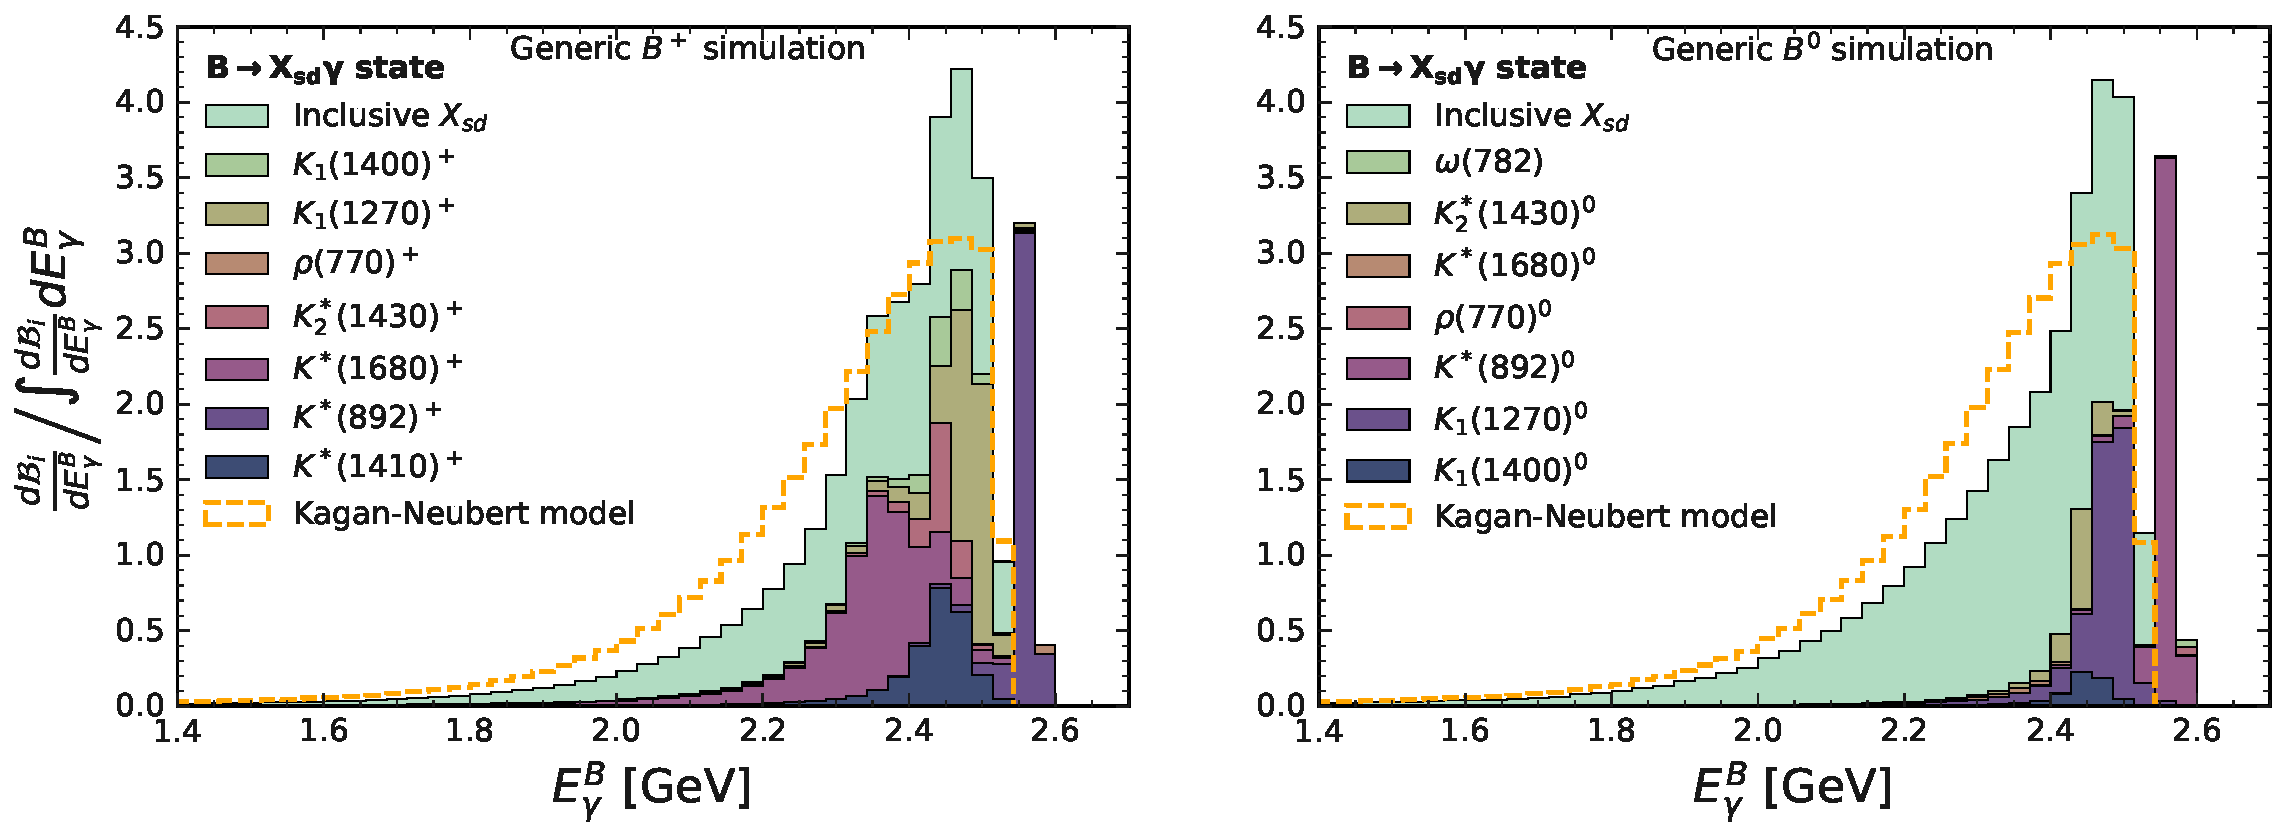
\includegraphics[width=0.95\textwidth]{figures/data_samples/generic_Xs_simulation.pdf}
    }
    }
    \subcaptionbox{\label{fig:generic_Xsz_model}}{
    \clipbox*{{0.5\width} {0\height} {1\width} {1\height}}{%
    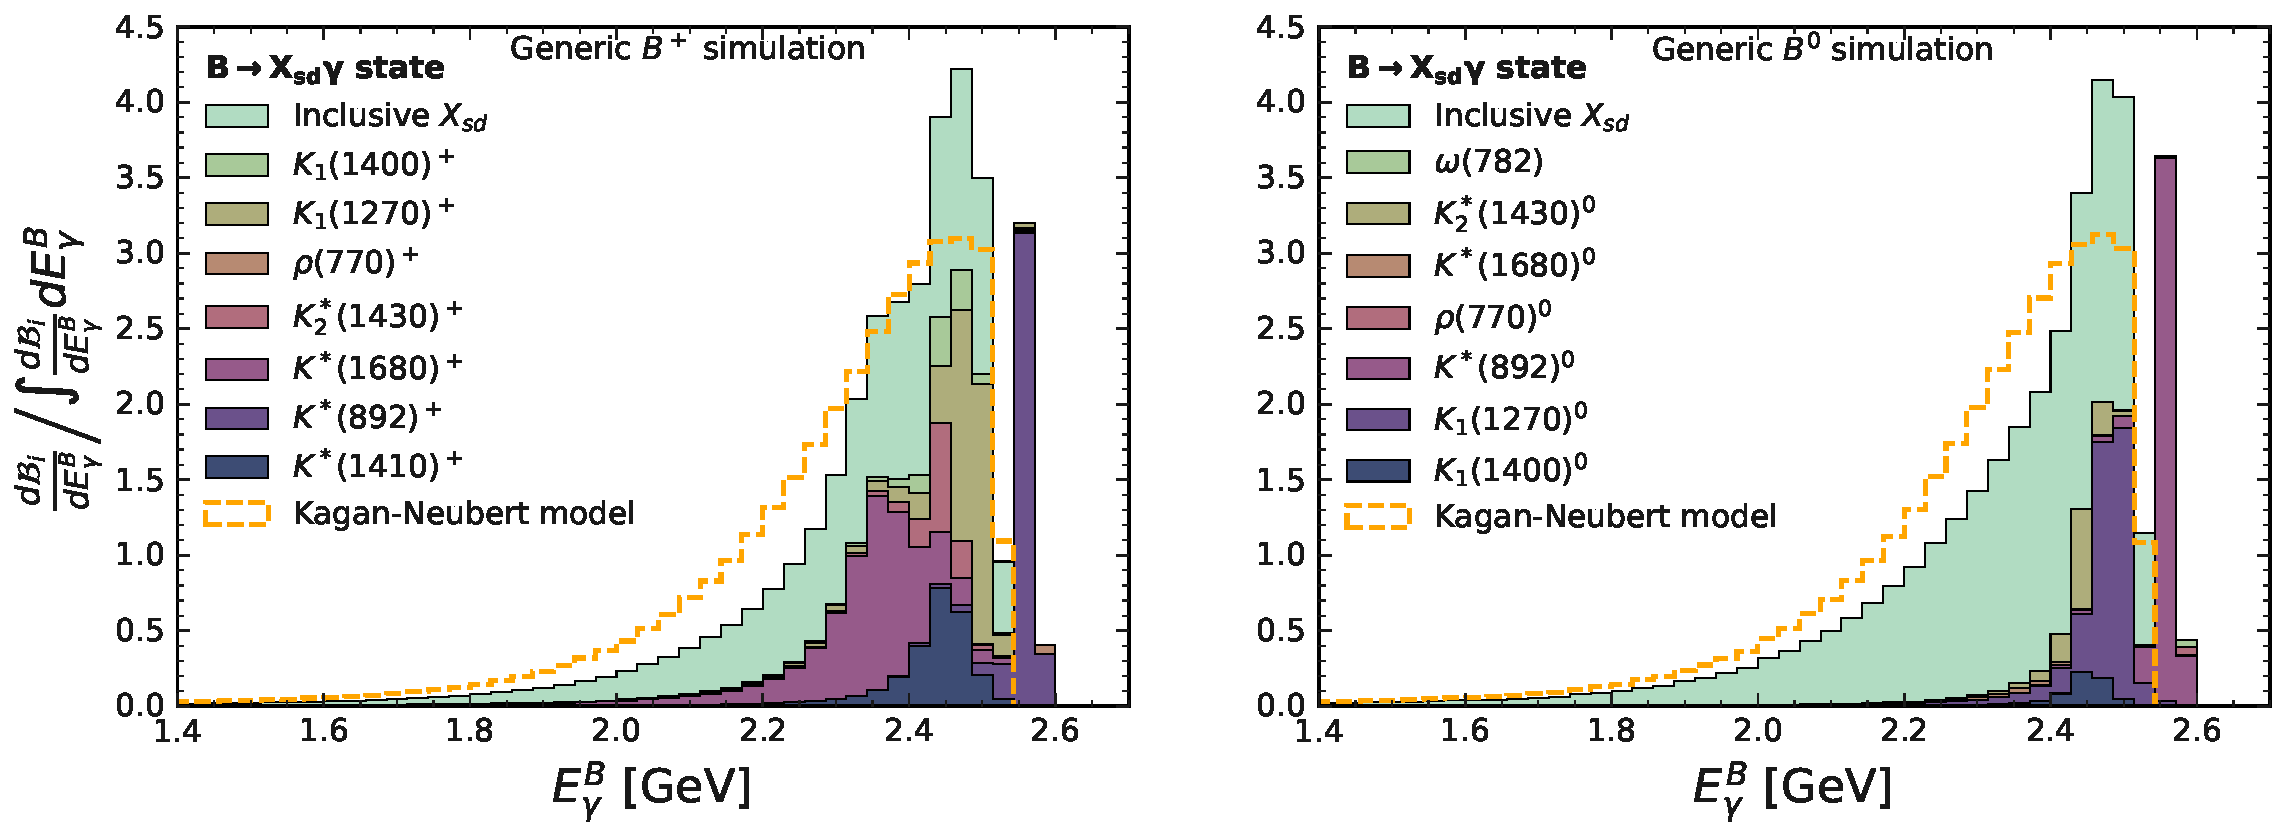
\includegraphics[width=0.95\textwidth]{figures/data_samples/generic_Xs_simulation.pdf}
    }
    }
    \caption{\label{fig:generic_Xs_model} The model for \BtoXsgamma used in the Belle II official generic-\Bp (\Cref{fig:generic_Xsp_model}) and generic-\Bz (\Cref{fig:generic_Xsz_model}) \MC.
    Although only several resonances are included, one can see that their structure is smoothed out.
    Unknown/unmeasured resonances as well as non-resonant decays are modelled with the inclusive Kagan-Neubert model, but the model is globally scaled down to account for the phase space covered by the exclusive decays.
    The branching fractions used here are taken from \Cref{tab:btosgamma_bfs} or upper-limits from Refs.\cite{Workman:2022ynf,Amhis:2022mac}.
    The dashed line shows the Kagan-Neubert Model.
    The figures are produced using 500 000 event data sets for each mode produced by \texttt{EvtGen} equivalently to the Belle II simulation.
    }    
\end{figure}

To ensure that the tail region is described correctly, while the resonant part is accounted for, a \textit{hybrid model} approach is prepared for this analysis.
It is implemented in a modified approach proposed by Ref.~\cite{Ramirez:1989yk}, where it was used for $\B\to X_u\ell\nu$.
The \BtoXsgamma photon energy spectrum is subdivided into multiple intervals, referred to as \textit{hybrid bins}.
The scaling, called \textit{hybrid weight}, instead of being global, is then calculated for each hybrid bin, such that:
\begin{equation}\label{eq:hybrid_model_definition}
    H_i = I_i\times h_i + \Sigma R_i,
\end{equation}
where $h_i$ is a hybrid weight for hybrid bin $i$; 
$I_i$ is the inclusive model prediction for the given hybrid bin; 
$\Sigma R_i$ is the prediction of all resonances in the hybrid bin;
$H_i$ is the hybrid model prediction in the hybrid bin.

As mentioned before, for the $I_i$ part, the Kagan-Neubert model is used (\Cref{sec:btosgamma_spectrum_theory}).
In order to use more up-to-date parameters of the spectrum, the spectrum is reweighted to be compatible with parameters from \Cref{eq:simba_result}.
In the kinetic scheme, compatible with \texttt{EvtGen} implementation of the Kagan-Neubert model, this amounts to:
\begin{equation}\label{eq:simba_result_kinetic}
    m_b^{kin} =4.624 \pm 0.045~\gevcc;  \quad \lambda^{\mathrm{kin}}_1 = -0.35\pm0.08~\gev^2/c^4.
\end{equation}
Taking into account the correlation of these parameters as described in Ref.~\cite{Bernlochner:2020jlt}, 4 additional up and down variations in the eigendirections are generated. 
The envelope of the variations is used as the inclusive model uncertainty in this analysis.
The reweighted inclusive model is shown in \Cref{fig:inclusive_reweighted}.
\begin{figure}[htbp!]
    \centering
    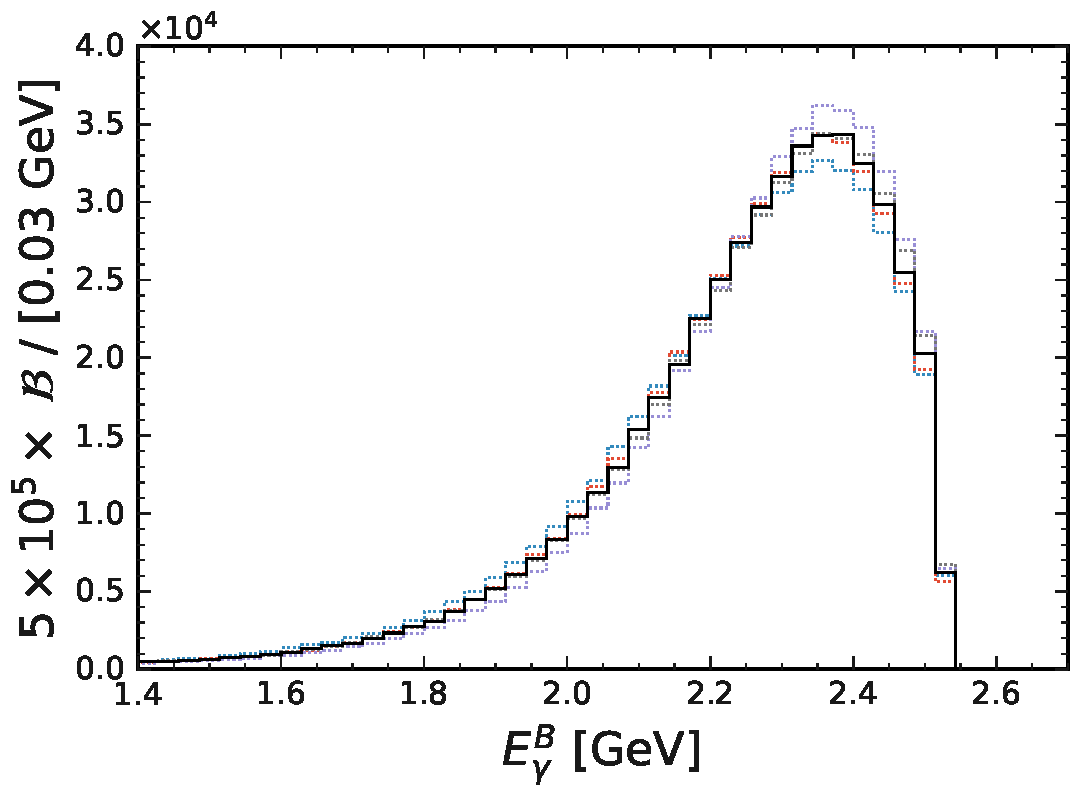
\includegraphics[width=0.45\textwidth]{figures/data_samples/xs_model_inclusive.pdf}
    \caption{\label{fig:inclusive_reweighted}The inclusive $X_s$ model based on \Cref{eq:simba_result_kinetic}.
    The dashed lines show 4 up and down $m_b$ and $\lambda_1$ variations based on their correlated uncertainties.
    The maximum deviations (envelope) are taken as the modelling uncertainty.}
\end{figure}

For the $R_i$ part, it was decided to only include the $B\rightarrow\Kstar(892)\gamma$ resonance.
The main reason to exclude other resonances is the fact that most are not known precisely, which would lead to a larger modelling uncertainty.
Furthermore, the expected statistical precision (see discussion in \Cref{sec:binning}) is not high enough to be sensitive to fine detail in the spectrum.

The set of hybrid bins was selected as displayed in \Cref{fig:hybrid_bins_and_model}.
An underflow and overflow bin is selected at $1.6$ and $2.3~\gev$, respectively.
The overflow bin is chosen to include the majority of the $\B\to\Kstar(892)\gamma$ resonance.
The finer 0.1~\gev-wide bins in between contain small amounts of $\B\to\Kstar(892)\gamma$ events.
In each \EB bin, an appropriate hybrid weight is calculated, such that the sum of the reweighted inclusive model (\Cref{fig:inclusive_reweighted}) and \mbox{$\B\to\Kstar(892)\gamma$} contribution matches the partial branching fraction within that \EB bin, based on \Cref{eq:hybrid_model_definition}.
This captures the desired description of the low-\EB region with the inclusive model, and a \Kstar(892)-dominated behaviour at high-\EB.

\begin{figure}[htbp!]
    \subcaptionbox{\label{fig:hybrid_binned_model}}{%
        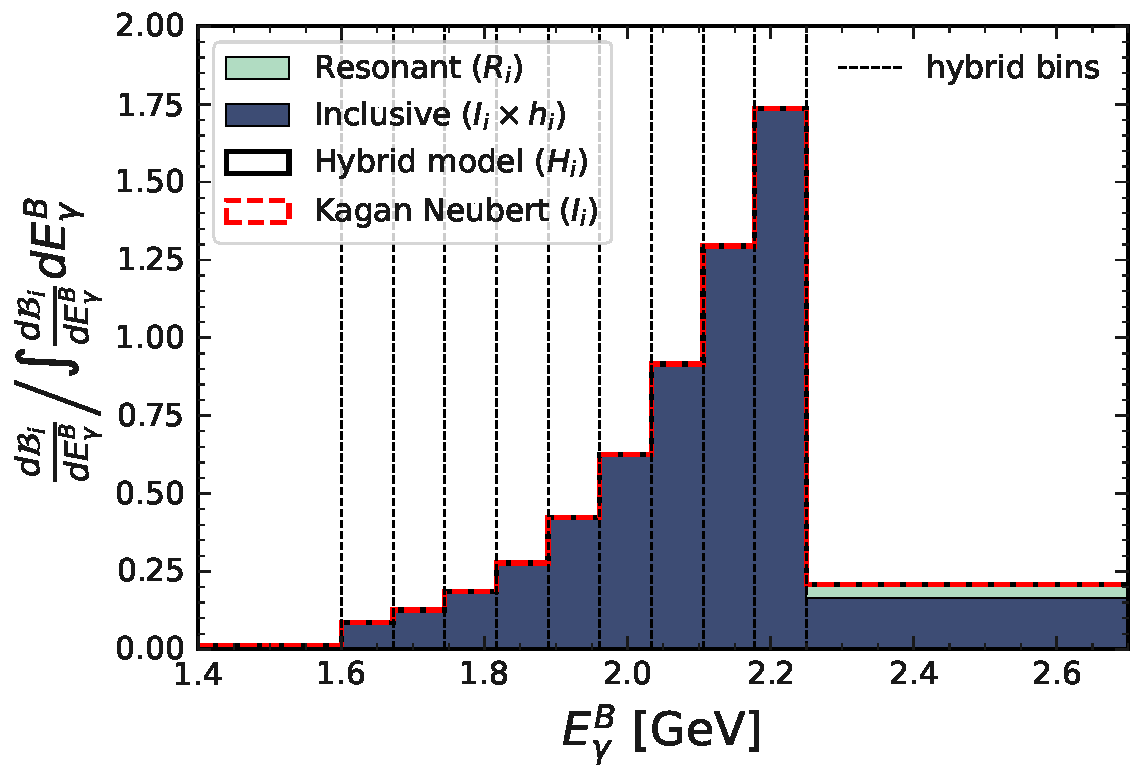
\includegraphics[width=0.45\textwidth]{figures/data_samples/normalised_signal_model_hybrid_binning.pdf}
    }
    \subcaptionbox{\label{fig:hybrid_binned_analysis_model}}{%
        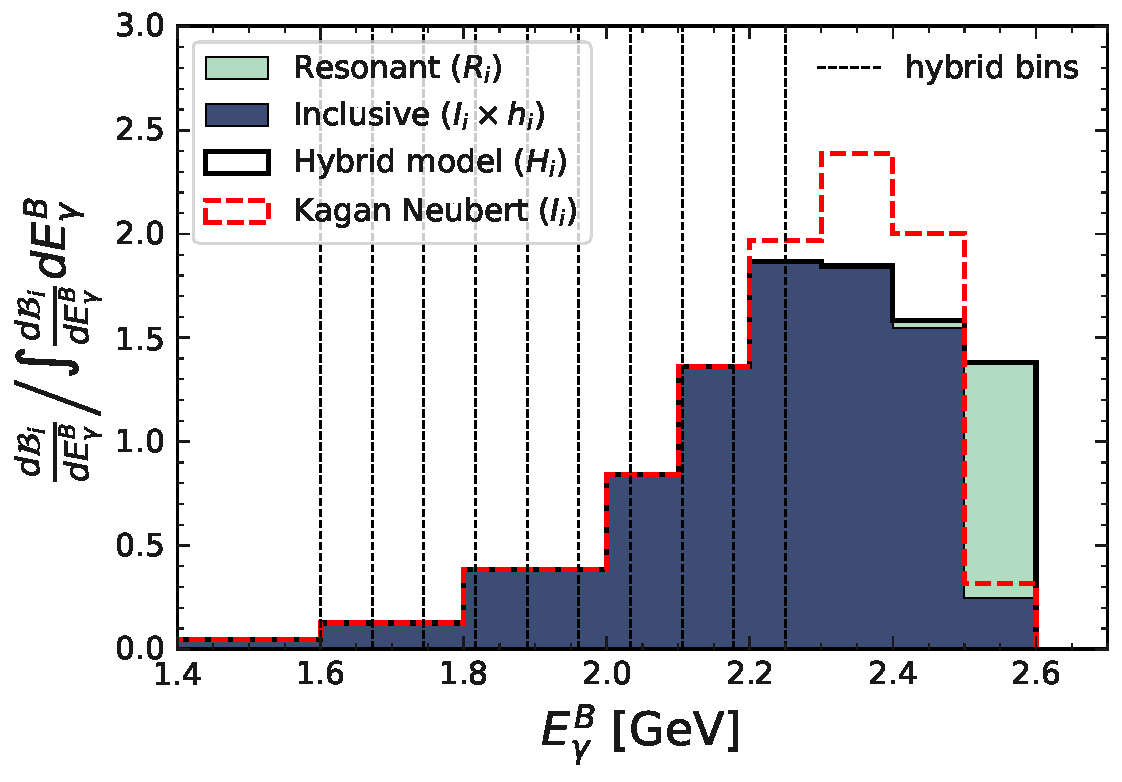
\includegraphics[width=0.45\textwidth]{figures/data_samples/normalised_signal_model.pdf}
        }
    \caption{\label{fig:hybrid_bins_and_model} The hybrid model constructed for this analysis 
    shown in two different binnings.
    \Cref{fig:hybrid_binned_model} shows it for a binning that matches the hybrid binning; 
    and \Cref{fig:hybrid_binned_analysis_model} shows it for a binning that will 
    be chosen in this analysis (see \Cref{sec:binning} and \Cref{tab:expected_events}).
    In both cases, the spectra are normalised such that the total area under them is 1.
    The hybrid model describes the tail adequately, 
    while also taking into account the resonant contributions (compare with \Cref{fig:generic_Xs_model}).
    The different components corresponding to \Cref{eq:hybrid_model_definition} are labelled appropriately.
    }
\end{figure}

The hybrid bins need not match the binning used in the analysis or plotting.
As seen in \Cref{fig:hybrid_binned_analysis_model}, the hybrid model can be used for different binnings which do not coincide with the hybrid bins.
In the Figure, the model is shown in the binning that will later be used for the analysis, after optimising based on expected signal and background contributions.

The uncertainty of the hybrid model is evaluated by taking into account:
\begin{itemize}
    \item Branching fraction uncertainty of the $\B\to\Kstar(892)\gamma$, $\sigma_{\mathrm{res}}$;
    \item Branching fraction uncertainty of the inclusive \BtoXsgamma decay, $\sigma_{\mathrm{incl}}$;
    \item Inclusive model parameter variation envelope, as shown in \Cref{fig:inclusive_reweighted}, $\sigma_{\mathrm{var}}$.
\end{itemize}
These components are evaluated based on the values discussed in this Section and \Cref{tab:btosgamma_bfs}.
They are visually shown for a selected \BtoXsgamma photon energy spectrum binning in \Cref{fig:hybrid_uncertainty}.
The uncertainty is dominated by \BtoXsgamma model variation uncertainties, except in the interval where $\B\ra\Kstar(892)\gamma$ dominates.
There the branching fraction uncertainty of the resonant decay is leading.
The uncertainty related to the \BtoXsgamma inclusive branching fraction model is smaller than the other two.
\begin{figure}[htbp!]
    \centering
    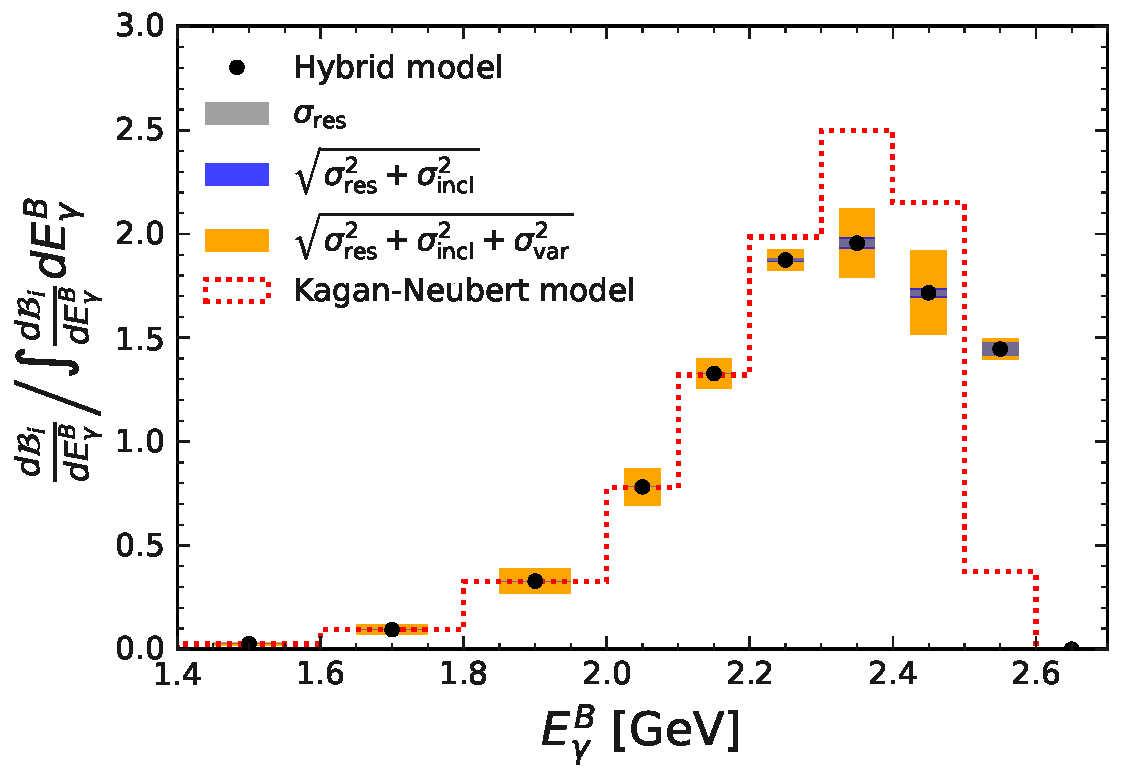
\includegraphics[width=0.45\textwidth]{figures/data_samples/hybrid_model_uncertainties.pdf}
    \caption{\label{fig:hybrid_uncertainty}The inclusive $X_s$ model based on \Cref{eq:simba_result_kinetic}
    overlaid with uncertainties from the resonant, inclusive branching fractions and the inclusive model parameters.
    The definitions of the uncertainties are given in the text.
    For comparison, the Kagan-Neubert model with the same parameters is also shown.
    }
\end{figure}




\section{Event reconstruction}\label{sec:event_reconstruction}

In the inclusive \BtoXsgamma analysis, the aim is to reconstruct an inclusive sample of all possible \Xs states, 
as described before (e.g. \Cref{ch:exp_overview}).
This means that explicit requirements on the momentum, number of tracks, angles etc. of the \Xs system may introduce a direct bias on the `inclusiveness' of the measurement.
Assessing the impact of such selections on $X_s$ in a model-independent way is difficult.
Therefore, the \Xs system is treated in a completely `missing-momentum' approach, such that no direct requirements on it are imposed.
The reconstruction requirements are only applied on the candidate tag-$B$ meson and the candidate high-energy photons from \BtoXsgamma.
\subsection{Tag-\texorpdfstring{$B$}{B} meson candidate reconstruction}\label{sec:tag_reconstruction}

The analysis begins with the reconstruction of tag-$B$ meson candidates in each event
using the Belle~II Full Event Intepretation (\FEI) algorithm \cite{Keck:2017mui,Keck:2018lcd}, which is part of \basftwo.
It is a hierarchical six-stage reconstruction chain, which begins with the identification of all tracks, displaced vertices (tracks that do not originate near the interaction point) and \ECL clusters.
The algorithm begins by combining track and ECL cluster information to reconstruct final-state candidate particles,
such as $\epm$, $\mupm$, $\gamma$,  $\pi^{\pm}$, $K^{\pm}$ and $K_L^0$.
In the next stage, the final-state particles are combined to form intermediate particles, such as $\piz, K_S^0, D^{(*)}$.
In later stages, intermediate and final-state particles are combined into $B$ mesons.
At every stage of the procedure, the probability for the combined particle to be correct is evaluated by a \BDT
which maps input features related to the particle (four-momentum, vertex position, angles between daughter particles etc.) to a single classifier
output score. The final output score related to the quality of reconstruction of the $B$ meson is denoted as \feiProb. 
The schematic visualisation of the reconstruction process is shown in \Cref{fig:fei_schematic}
\begin{figure}[htbp!]
    \centering
    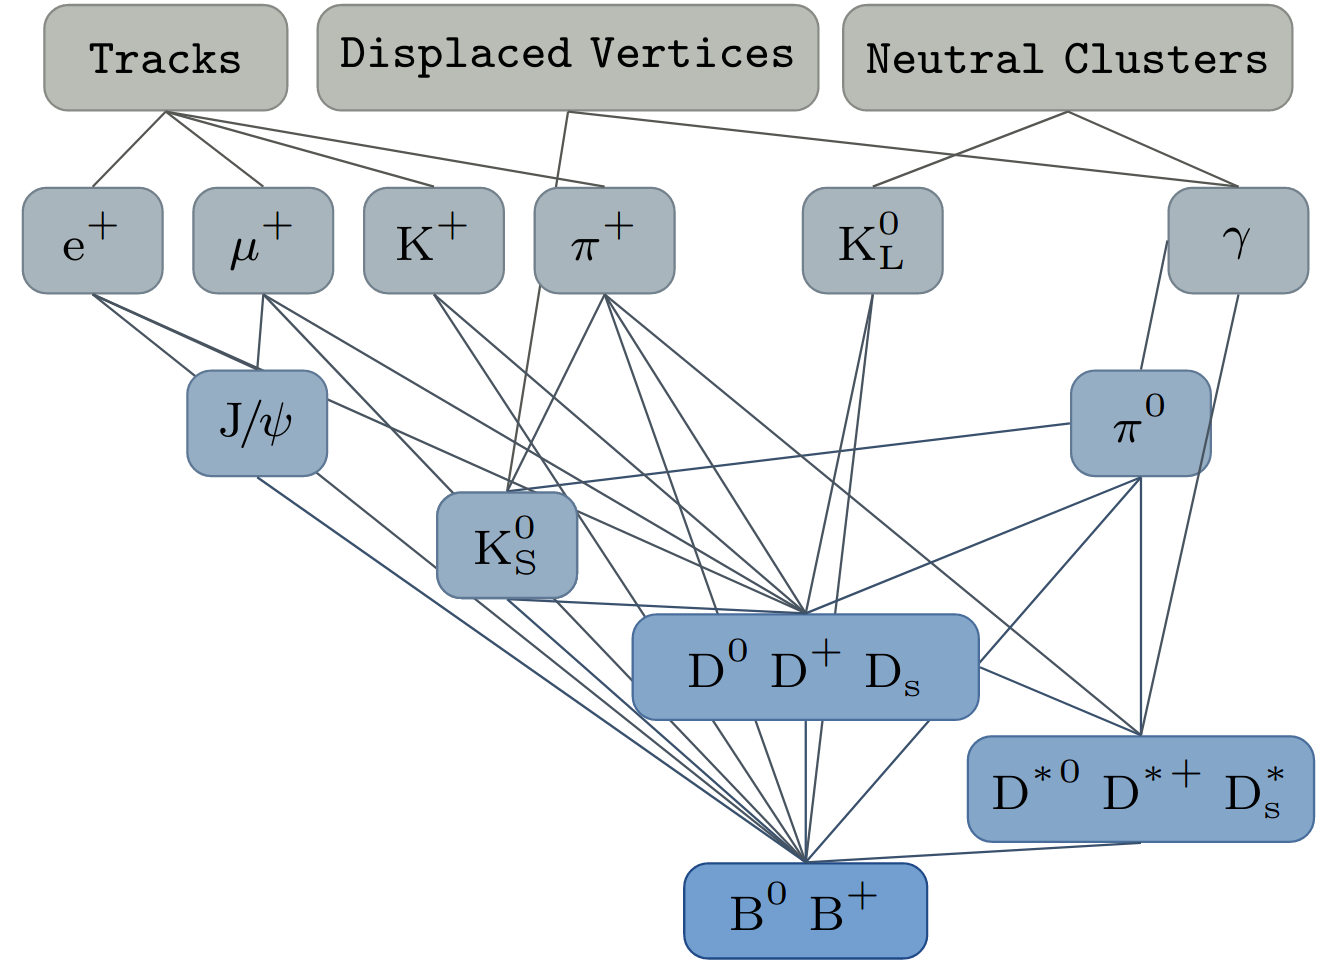
\includegraphics[width=0.45\textwidth]{figures/event_reconstruction/FEI_tagging.png}
    \caption{\label{fig:fei_schematic} 
    The schematic overview of \FEI.
    The algorithm reconstructs $B^+$ ($B^0$) candidates in 36 (32) hadronic decay chains
    in six reconstruction stages that combine final-state and intermediate particles.
    Credit to Ref.~\cite{Keck:2018lcd}.
    }
\end{figure}

In total, \FEI reconstructs $\order(10000)$ distinct decay chains and provides $B^+$ meson candidates in 36 hadronic decay modes, and $B^0$ candidates in 32 hadronic decay modes.
As a result, two \FEI modes are differentiated: 
\feiBp, which combines \Bpm meson candidates;
and \feiBz, which combines \Bz meson candidates.
Each event may have more than one candidate reconstructed in the same and/or different decay channels and/or \FEI modes.
The reconstructed decay channels for \feiBp and \feiBz modes are shown in \Cref{tab:fei_modes}.

\begin{table}
    \centering
    \caption{\label{tab:fei_modes}
    The $B$ meson decay modes reconstructed by the \FEI algorithm.
    \FEI modes reconstructed as \feiBp and \feiBz are listed separately.
    }
    \begin{tabular}{|l|l|l|}
    \hline
    &\feiBp modes & \feiBz modes\\
    \hline
    1.&$B^{+} \rightarrow \bar{D}^{0} \pi^{+}$                         &     $B^{0} \rightarrow D^{-} \pi^{+}$ \\
    2.&$B^{+} \rightarrow \bar{D}^{0} \pi^{+} \pi^{0}$                 &     $B^{0} \rightarrow D^{-} \pi^{+} \pi^{0}$ \\
    3.&$B^{+} \rightarrow \bar{D}^{0} \pi^{+} \pi^{0} \pi^{0}$         &     $B^{0} \rightarrow D^{-} \pi^{+} \pi^{0} \pi^{0}$\\
    4.&$B^{+} \rightarrow \bar{D}^{0} \pi^{+} \pi^{+} \pi^{-}$         &     $B^{0} \rightarrow D^{-} \pi^{+} \pi^{+} \pi^{-}$\\
    5.&$B^{+} \rightarrow \bar{D}^{0} \pi^{+} \pi^{+} \pi^{-} \pi^{0}$  &     $B^{0} \rightarrow D^{-} \pi^{+} \pi^{+} \pi^{-} \pi^{0}$\\
    6.&$B^{+} \rightarrow \bar{D}^{0} D^{+}$                           &     $B^{0} \rightarrow \bar{D}^{0} \pi^{+} \pi^{-}$\\
    7.&$B^{+} \rightarrow \bar{D}^{0} D^{+} K_{S}^{0}$                 &     $B^{0} \rightarrow D^{-} D^{0} K^{+}$\\
    8.&$B^{+} \rightarrow \bar{D}^{0 *} D^{+} K_{S}^{0}$               &     $B^{0} \rightarrow D^{-} D^{0 *} K^{+}$\\
    9.&$B^{+} \rightarrow \bar{D}^{0} D^{+*} K_{S}^{0}$                &     $B^{0} \rightarrow D^{-*} D^{0} K^{+}$\\
    10.&$B^{+} \rightarrow \bar{D}^{0 *} D^{+*} K_{S}^{0}$              &     $B^{0} \rightarrow D^{-*} D^{0 *} K^{+}$\\
    11.&$B^{+} \rightarrow \bar{D}^{0} D^{0} K^{+}$                     &     $B^{0} \rightarrow D^{-} D^{+} K_{S}^{0}$\\
    12.&$B^{+} \rightarrow \bar{D}^{0 *} D^{0} K^{+}$                   &     $B^{0} \rightarrow D^{-*} D^{+} K_{S}^{0}$\\
    13.&$B^{+} \rightarrow \bar{D}^{0} D^{0 *} K^{+}$                   &     $B^{0} \rightarrow D^{-} D^{+*} K_{S}^{0}$\\
    14.&$B^{+} \rightarrow \bar{D}^{0 *} D^{0 *} K^{+}$                 &     $B^{0} \rightarrow D^{-*} D^{+*} K_{S}^{0}$\\
    15.&$B^{+} \rightarrow D_{s}^{+} \bar{D}^{0}$,                      &       $B^{0} \rightarrow D_{s}^{+} D^{-}$\\
    16.&$B^{+} \rightarrow \bar{D}^{0 *} \pi^{+}$                       &     $B^{0} \rightarrow D^{-*} \pi^{+}$\\
    17.&$B^{+} \rightarrow \bar{D}^{0 *} \pi^{+} \pi^{0}$               &     $B^{0} \rightarrow D^{-*} \pi^{+} \pi^{0}$\\
    18.&$B^{+} \rightarrow \bar{D}^{0 *} \pi^{+} \pi^{0} \pi^{0}$       &     $B^{0} \rightarrow D^{-*} \pi^{+} \pi^{0} \pi^{0}$\\
    19.&$B^{+} \rightarrow \bar{D}^{0 *} \pi^{+} \pi^{+} \pi^{-}$       &     $B^{0} \rightarrow D^{-*} \pi^{+} \pi^{+} \pi^{-}$\\
    20.&$B^{+} \rightarrow \bar{D}^{0 *} \pi^{+} \pi^{+} \pi^{-} \pi^{0}$&     $B^{0} \rightarrow D^{-*} \pi^{+} \pi^{+} \pi^{-} \pi^{0}$\\
    21.&$B^{+} \rightarrow D_{s}^{+*} \bar{D}^{0}$                      &     $B^{0} \rightarrow D_{s}^{+*} D^{-}$\\
    22.&$B^{+} \rightarrow D_{s}^{+} \bar{D}^{0 *}$                     &     $B^{0} \rightarrow D_{s}^{+} D^{-*}$\\
    23.&$B^{+} \rightarrow \bar{D}^{0} K^{+}$                           &     $B^{0} \rightarrow D_{s}^{+*} D^{-*}$\\
    24.&$B^{+} \rightarrow D^{-} \pi^{+} \pi^{+}$                       &     $B^{0} \rightarrow J / \psi K_{S}^{0}$\\
    25.&$B^{+} \rightarrow D^{-} \pi^{+} \pi^{+} \pi^{0}$               &      $B^{0} \rightarrow J / \psi K^{+} \pi^{-}$\\
    26.&$B^{+} \rightarrow J / \psi K^{+}$                              &    $B^{0} \rightarrow J / \psi K_{S}^{0} \pi^{+} \pi^{-}$\\
    27.&$B^{+} \rightarrow J / \psi K^{+} \pi^{+} \pi^{-}$              &     $B^{0} \rightarrow \Lambda_{c}^{-} p \pi^{+} \pi^{-}$\\
    28.&$B^{+} \rightarrow J / \psi K^{+} \pi^{0}$                      &     $B^{0} \rightarrow \bar{D}^{0} p \bar{p}$\\
    29.&$B^{+} \rightarrow J / \psi K_{S}^{0} \pi^{+}$                  &     $B^{0} \rightarrow D^{-} p \bar{p} \pi^{+}$\\
    30.&$B^{+} \rightarrow \Lambda_{c}^{-} p \pi^{+} \pi^{0}$           &     $B^{0} \rightarrow D^{-*} p \bar{p} \pi^{+}$\\
    31.&$B^{+} \rightarrow \Lambda_{c}^{-} p \pi^{+} \pi^{-} \pi^{+}$   &     $B^{0} \rightarrow \bar{D}^{0} p \bar{p} \pi^{+} \pi^{-}$\\
    32.&$B^{+} \rightarrow \bar{D}^{0} p \bar{p} \pi^{+}$               &     $B^{0} \rightarrow \bar{D}^{0 *} p \bar{p} \pi^{+} \pi^{-}$\\
    33.&$B^{+} \rightarrow \bar{D}^{0 *} p \bar{p} \pi^{+}$             &     \\
    34.&$B^{+} \rightarrow D^{+} p \bar{p} \pi^{+} \pi^{-}$             & \\
    35.&$B^{+} \rightarrow D^{+*} p \bar{p} \pi^{+} \pi^{-}$            & \\ 
    36.& $B^{+} \rightarrow \Lambda_{c}^{-} p \pi^{+}$                   & \\
    \hline
\end{tabular}
\end{table}


This thesis uses data and simulation samples following the standard Belle~II approach, where sub-samples of data and \MC with the FEI algorithm applied are produced centrally, referred to as \textit{\FEI skims}.
In order to make the \FEI algorithm more computationally efficient, event selections are made to reject events highly incompatible with one of the $B$ mesons decaying hadronically.
This decision is based on tracks and clusters as per standard Belle~II reconstruction guidelines with additional selections, summarised in \Cref{tab:fei_objects}.
Overeall, they ensure that only energetic tracks originating from the interaction point are selected.
They also minimise the impact of beam background clusters or clusters for which no track information can be associated (outside of \CDC acceptance).

\begin{table}[htbp!]
    \centering
     \caption{\label{tab:fei_objects} Definitions for objects used in \FEI selections.}
     \resizebox{0.75\textwidth}{!}{
     \begin{tabular}{|l|c|c|} 
        \hline

     Selection description & Selection\\
     \hline
     Cleaned tracks & $  |d_0|<0.5~\cm,\quad z_0<2~\cm,\quad p_T>0.1~\gev $\\
     Cleaned \ECL clusters & $17~\degrees<\theta<150~\degrees,\quad E>0.1~\gev$\\
     \hline

     \end{tabular}
     }
\end{table}
Using the definitions of cleaned tracks and \ECL clusters, reconstructed events are filtered and only the events that pass the requirements are analysed by the \FEI algorithm.
Such requirements are summarised in \Cref{tab:fei_precuts}.

\begin{table}[htbp!]
    \centering
     \caption{\label{tab:fei_precuts} Selections before running the \FEI algorithm.
     Cleaned tracks and clusters are defined in \Cref{tab:fei_objects}.
     }
     \resizebox{0.75\textwidth}{!}{
     \begin{tabular}{|l|c|} 
    \hline
     Selection description & Selection\\
     \hline
     Number of cleaned tracks in event \quad & $\geq 3$\\
     Number of cleaned \ECL clusters in event \quad & $\geq 3$\\
     Total measured centre-of-mass energy in the event \quad & $> 4~\gev$\\
     Total energy of cleaned \ECL clusters \quad &\multirow{2}{*}{$2~\gev<E<7~\gev$}\\
     and deposits associated with cleaned tracks \quad & \\
     \hline
    \end{tabular}
     }
\end{table}
The selection of events with at least 3 cleaned tracks in the event and at least 3 cleaned \ECL clusters is based on the fact, that \BB events produce $\sim10$ charged tracks and neutral particles~\cite{BaBar:2014omp}.
Furthermore, the measured energy of the event is required to exceed 4~\gev in the \epem collision centre-of-mass frame.
This is a purely pragmatic requirement: because no neutrinos or missing-momentum are present in a hadronic decay, the energy cannot be much lower than 5.28~\gev.
Finally, the total deposited energy registered by the \ECL in the event is required to be between 2 and 7~\gev.
Hadronic events are expected to deposit significantly more energy than 2~\gev.
On the other hand, many lower-energetic particles should be stopped within \PXD, \SVD, \CDC or \TOP, meaning that their energy deposit in the \ECL would be negligible.
Therefore, a 7~\gev \ECL energy upper limit ensures that low-multiplicity events, such as \epem\ra\epem, are immediately removed to ensure a better-optimised workflow.

The events that pass the requirements of \Cref{tab:fei_precuts} are analysed by the \FEI algorithm.
In each event, multiple \FEI candidates can be reconstructed (see \Cref{fig:fei_tag_reco_candidates}).
To focus only on the candidates that have been correctly reconstructed, selections on \DeltaE and \Mbc are made, as well as a loose requirement on \feiProb.
The selections shown in \Cref{tab:fei_skim_cuts} are standard selections that are applied on the Belle~II \FEI skims.

\begin{table}[htbp!]
    \centering
     \caption{\label{tab:fei_skim_cuts} 
     Additional selections that reduce the datasets after applying \FEI, focusing only on well-reconstructed tag-side candidates.
     These \FEI skim selections are the nominal ones, which are applied on all \FEI skimmed data sets in Belle~II.
     In this analysis, only the selection on the tag-\B meson is tightened in order to remove the edge effects.
     Such effects arise after applying a kinematic fit on the tag-side products.
     }
     \resizebox{0.75\textwidth}{!}{
        \begin{tabular}{|l|c|c|}
        \hline
        Variable &    \FEI skim selections  & Selections in this analysis \\
        \hline
        $\Mbc (\mathrm{tag})$ & $>5.24~\gev$ & $>5.245~\gev$  \\
        $\Delta E (\mathrm{tag})$ & \multicolumn{2}{c|}{$-0.15$ to $0.1$~\gev} \\
        \feiProb E & \multicolumn{2}{c|}{$> 0.001$}\\
        
        \hline
        
\end{tabular}
    
     }
\end{table}

The tag-side candidates that pass the nominal \FEI requirements undergo a kinematic fit \cite{Belle-IIanalysissoftwareGroup:2019dlq}, 
where the particles used to reconstruct the tag-$B$ candidate are fitted with a common vertex constraint.
No requirements on the quality of the fit are made, but candidates that fail the fit are rejected.
This improves the resolution of the $B$ meson momentum for correct candidates and may shift their momentum altogether.
Therefore, to avoid distribution-edge effects, a tighter \Mbc selection is used in this analysis, as illustrated in \Cref{tab:fei_skim_cuts}.
The tag-side selections used in this analysis are not affecting the \BtoXsgamma, 
as correct tag-side candidates with 
lower \Mbc, 
higher $|\DeltaE|$ 
or lower \feiProb (compared to \Cref{tab:fei_skim_cuts}) are not expected to be common.


\subsection{Candidate photon reconstruction}\label{sec:gamma_reconstruction}

Only the photon from \BtoXsgamma can be reconstructed while ensuring a model-independent inclusive measurement.
In order to reduce the quickly growing number of background photon candidates, only events where at least one photon with $\Estar>1.2~\gev$ are considered.
Photons must also be within the \CDC acceptance ($17-150~\degrees$).
These requirements are summarised in \Cref{tab:photon_requirements}.
Reconstructed photon energy is boosted to the signal $B$ meson rest frame based on the Lorentz transformation in \Cref{sec:appendix_boosting_to_b_frame}.
\begin{table}[htbp!]
    \centering
     \caption{\label{tab:photon_requirements} Requirements for photons in reconstructed events.}
     \resizebox{0.75\textwidth}{!}{
     \begin{tabular}{|l|c|}
     \hline 
     Selection description & Selection\\
     \hline
     Number of photons with \Estar>1.2~\gev & $  N(\Estar>1.2~\gev)\geq1 $\\
     Polar angle of photon & $17~\degrees<\theta<150~\degrees$\\
     \hline
     \end{tabular}
     }
\end{table}

\subsection{Overview of the selected sample}\label{sec:reconstruction_overview}

After the reconstruction, based on the \MC samples, there can be up to 20 tag-$B$ candidates.
The sample is broken down to show the relative fraction of the total number of tag-side $B$ meson candidates in 
\Cref{fig:fei_tag_reco_candidates}.
About 62\% (72\%) of events for \feiBp (\feiBz) modes have only 1 tag-side candidate.
About 21\% (18\%) of events for \feiBp (\feiBz) modes have two tag-side candidates, and 8\% (5\%) have 3.
The number of candidates per event reduces quickly, but faster for \Bz modes, with roughly 2\% (1\%) 
of events having more than 5 candidates for \feiBp (\feiBz).
Note that the same event can have a \Bp and \Bz candidate reconstructed.

A similar distribution for the number of signal-side photon candidates with a threshold of $\EB>1.4~\gev$ is shown in \Cref{fig:photon_reco_candidates}.
The highest energy photon is the sole candidate in the event in 98\% of the cases in generic \MC.
Studies on \BtoXsgamma signal \MC with a threshold of $\EB>1.4~\gev$ show that a single high-energy photon is expected in 99.9\% of the cases.
The $\EB>1.4~\gev$ selection is chosen pragmatically to maintain a reasonable data set memory size without losing signal events.
As the number of photon candidates grows swiftly with decreasing energy, this threshold still provides access to the majority of the \BtoXsgamma decay phase space.
\begin{figure}[htbp!]
    \centering
    \subcaptionbox{\label{fig:fei_tag_reco_candidates}}{
    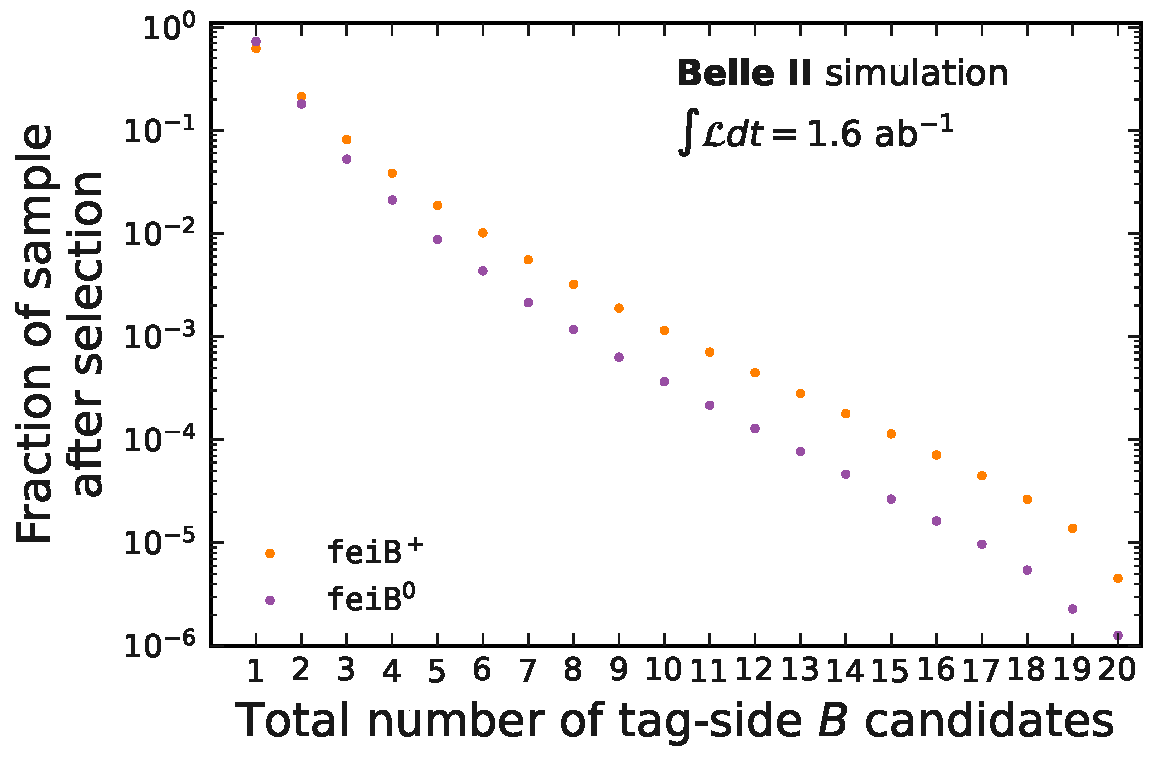
\includegraphics[width=0.45\textwidth]{figures/event_reconstruction/Bboth_total_tag_candidates.pdf}
    }
    \subcaptionbox{\label{fig:photon_reco_candidates}}{
        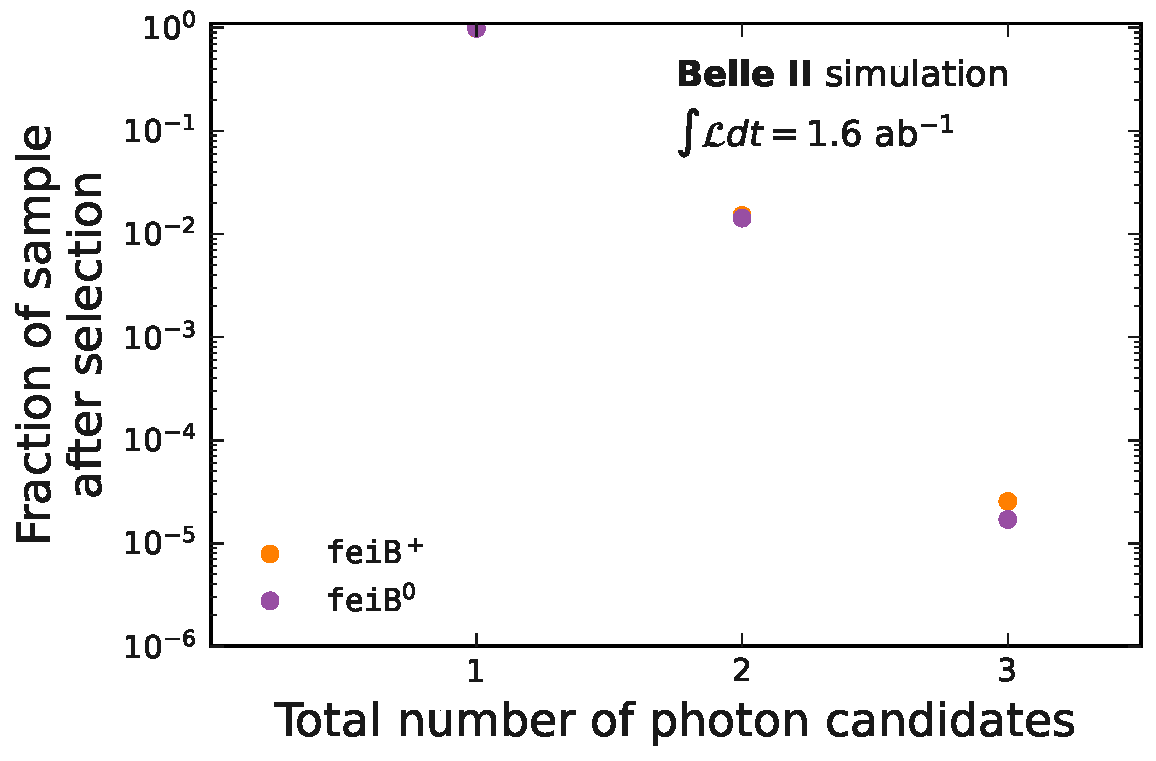
\includegraphics[width=0.45\textwidth]{figures/event_reconstruction/Bboth_total_photon_candidates.pdf}
    }
    \caption{\label{fig:reco_candidates} Relative fractions of events for the number of 
    reconstructed \B meson candidates (\Cref{fig:fei_tag_reco_candidates}) and
    reconstructed photon candidates (\Cref{fig:photon_reco_candidates}) in the generic \MC sample.
    In \Cref{fig:fei_tag_reco_candidates}, the overall volume of candidates is similar for \feiBp and \feiBz modes, 
    with around one in two events only having a single candidate per event.
    Conversely, as depicted in \Cref{fig:photon_reco_candidates},
    the vast majority of events contain only a single signal photon with $\EB>1.4~\gev$.
    Two or more photon candidates are present only $\mathcal{O}(1)\%$ of the time.
    }
\end{figure}

The reconstructed \BtoXsgamma spectrum in generic \MC with the previously laid-out requirements are shown in \Cref{fig:spectrum_after_reco}.
Note that these events in general can contain multiple combinations of a photon and tag-side candidate per event.
Overall, it may seem that the \feiBz mode has a higher signal-to-background ratio compared to \feiBp.
However, one has to take into account that \feiBp and \feiBz modes result
from different reconstruction chains.
Furthermore, \feiBz has fewer modes than \feiBp (see \Cref{sec:tag_reconstruction}).
Therefore, without additional studies that follow in \Cref{sec:select_tag_between_modes,sec:select_best_candidate} such a conclusion cannot be unambiguously drawn. 
On the other hand, by looking at \Cref{fig:untagged_btosgamma_background,fig:spectrum_after_reco}, it is clear that a better signal-to-background ratio can already be observed even without any additional background treatment.

\begin{figure}[htbp!]
    \centering
    \subcaptionbox{\label{fig:spectrum_after_reco_bplus}}{
        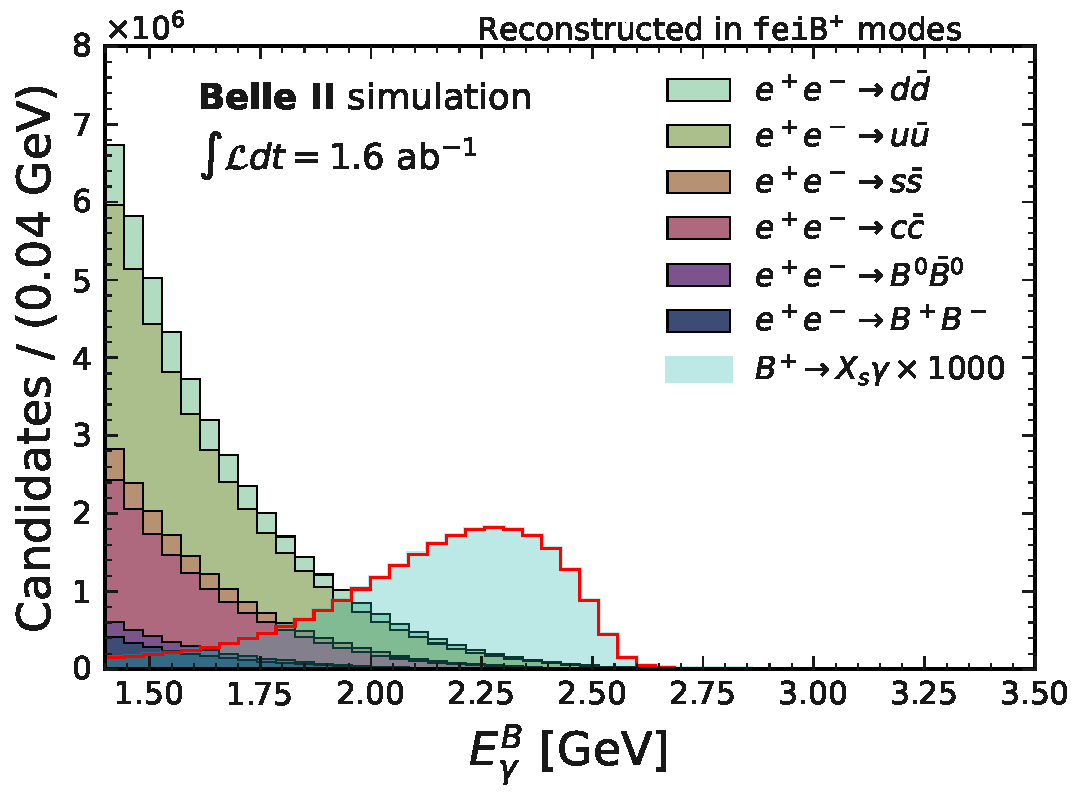
\includegraphics[width=0.45\textwidth]{figures/event_reconstruction/Bp_tagged_background.pdf}
        }
    \subcaptionbox{\label{fig:spectrum_after_reco_bzero}}{
    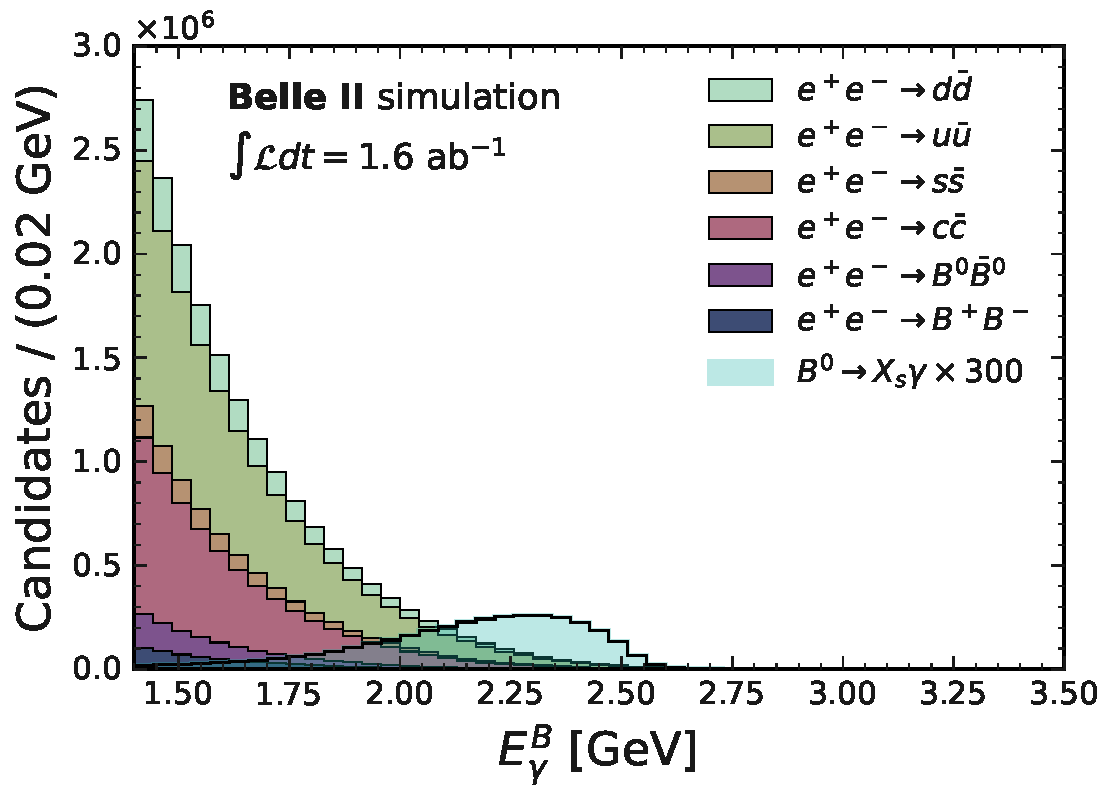
\includegraphics[width=0.45\textwidth]{figures/event_reconstruction/Bz_tagged_background.pdf}
    }
    \caption{\label{fig:spectrum_after_reco} \BtoXsgamma spectrum in generic \MC after event reconstruction in \feiBp and \feiBz modes.
    Overlaid are events from signal \MC, where the photon comes from \BtoXsgamma, multiplied by a scaling factor.
    These figures may include multiple tag-$B$ and photon entries per event and can be compared with \Cref{fig:untagged_btosgamma_background}.
    }
\end{figure}

The tag-side probability distributions provided by the \FEI classifier are shown in \Cref{fig:sigprob_after_reco}.
They further emphasise the differences between tag candidates reconstructed in \feiBp and \feiBz modes.
A selection on the \feiProb variable is not trivial;
even after disregarding the differences between \feiBp and \feiBz modes, 
the \feiProb values may be different within the same-charged $B$ mode.
This is shown and discussed in \Cref{sec:appendix_fei_signal_probabilities}.
Tight direct selections, as seen in \Cref{fig:feisigprobs1,fig:feisigprobs2,fig:feisigprobs3,fig:feisigprobs4}, result in a bias for selected tag-side modes.
Therefore, no direct selections on \feiProb are applied in this analysis.

\begin{figure}[htbp!]
    \centering
    \subcaptionbox{\label{fig:sigprob_after_reco_bplus}}{
        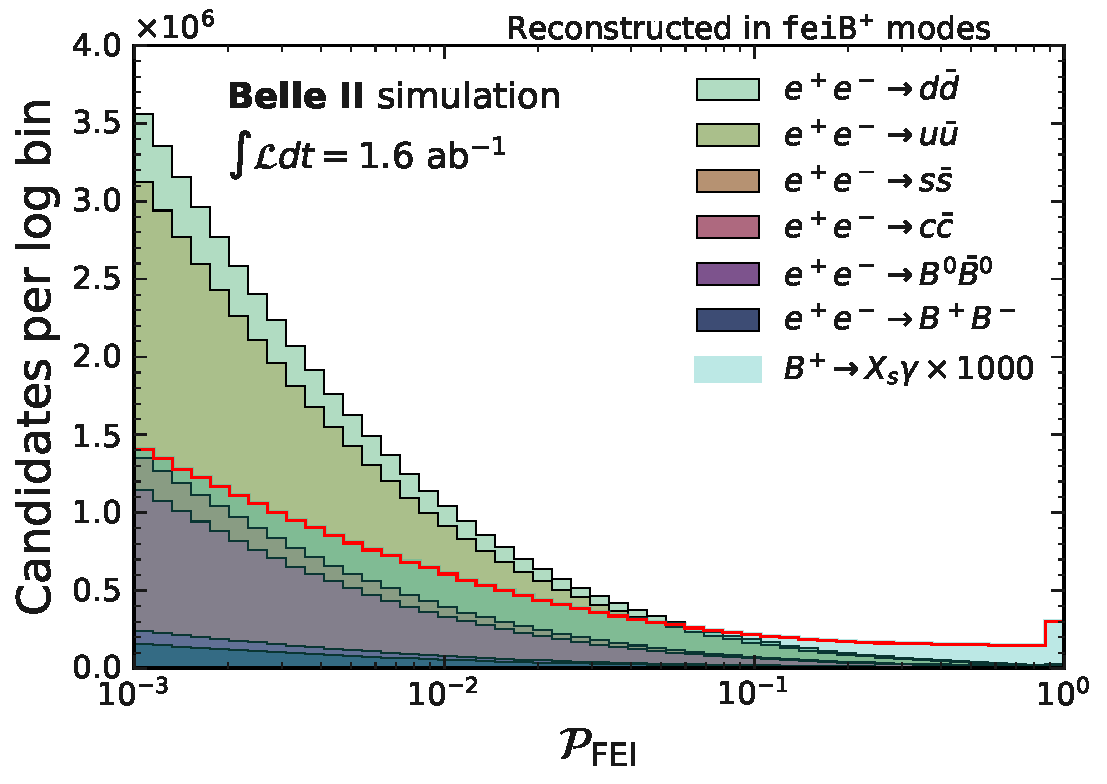
\includegraphics[width=0.45\textwidth]{figures/event_reconstruction/Bp_tagged_background_feiSigProb.pdf}
        }
    \subcaptionbox{\label{fig:sigprob_after_reco_bzero}}{
    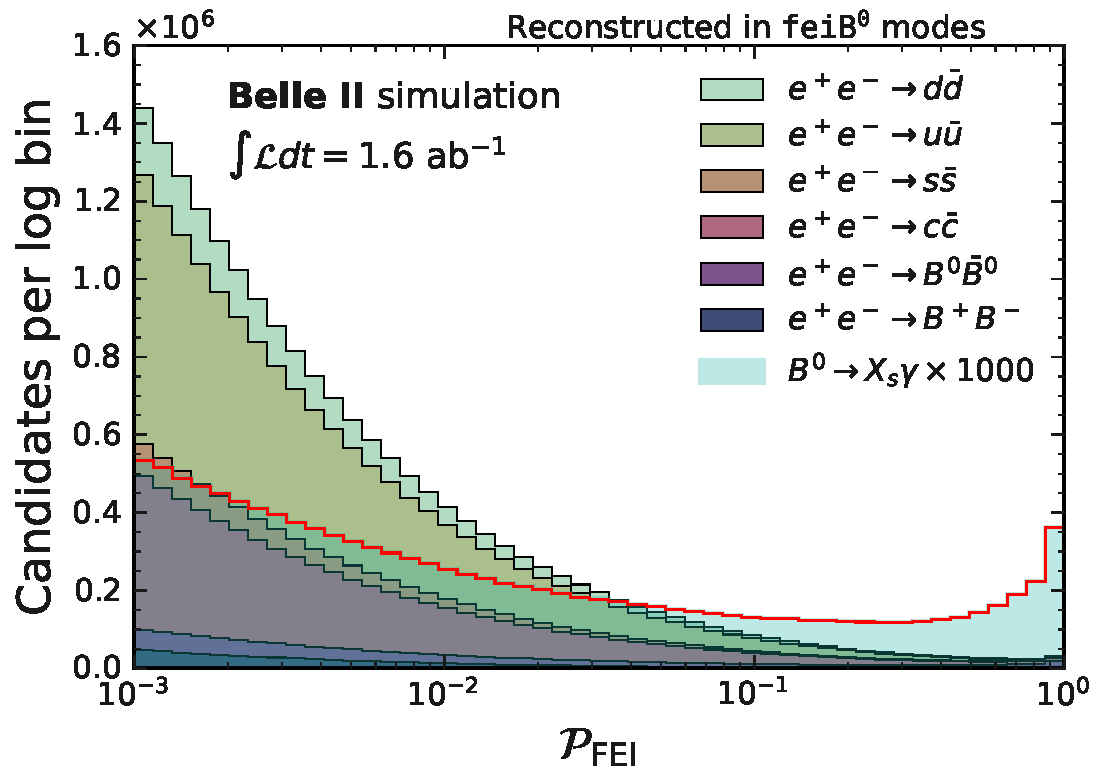
\includegraphics[width=0.45\textwidth]{figures/event_reconstruction/Bz_tagged_background_feiSigProb.pdf}
    }
    \caption{\label{fig:sigprob_after_reco} Tag-side \feiProb after reconstructing \BtoXsgamma events in generic \MC in \feiBp and \feiBz modes.
    Overlaid are events from signal \MC, where the photon comes from \BtoXsgamma, multiplied by a scaling factor.
    These figures may include multiple tag-$B$ and photon entries per event.
    }
\end{figure}

% \subsection{Event topology reconstrunction}
% Many quantities that parametrise the \epem collision product topology in terms of tracks and neutral clusters in the event will be used.
% Using a definition, equivalent to cleaned tracks and clusters we recon

\section{Photon candidate selection}\label{sec:photon_selection}
The previous Section overviewed the samples that are reconstructed using basic requirements laid out in \Cref{sec:tag_reconstruction,sec:gamma_reconstruction}.
In this Section concrete selections are discussed that lead to background suppression, the best photon candidate
and the best tag candidate selections.

\subsection{Primary photon candidate selection}\label{sec:primary_photon_candidate_selection}
Contrary to the tag-side, a selection of the best photon candidate in the range $\EB>1.4~\gev$ 
is effectively trivial based on the discussion in \Cref{sec:event_reconstruction}.
For more than 99\% of the signal \MC sample, the highest \EB photon 
is the correct photon originating from \BtoXsgamma decay.
Therefore, it is chosen as the best photon candidate requirement with virtually no signal efficiency loss.
Judging from \Cref{fig:photon_reco_candidates}, this provides an approximately 3\% background suppression.
For the rest of the thesis, this selection is always implied when referring to signal-photon candidates.

\subsection{Main photon background sources}\label{sec:main_background_sources}

Based on \Cref{fig:spectrum_after_reco}, the number of photon and tag candidates originating 
in non-\BB events is significantly larger than that of \B meson events.
The proportion of \qqbar to \BB event candidates is 92.5\% to 7.5\% for \feiBp mode;
and 91.7\% to 8.3\% for \feiBz.

The majority of background photon candidates originate in $\piz\ra\g\g$ or $\eta\ra\g\g$ decays.
This in total accounts for roughly 85\% of background photon candidates.
Photon candidates, broken down by their mother particle, are shown in \Cref{fig:photon_sources}.
Other sources, such as (in decreasing order) initial-state radiation, neutron annihilation, parton shower final-state radiation, $\omega(782)$, $\eta'$ decays each make up $0.5-3\%$ of the sample.
All other sources individually make up less than 0.5\% and include various hadron decays that are produced in continuum or \B events.
The backgrounds are similar for both \feiBp and \feiBz modes.
Note that some photon candidates can be misidentified, in particular neutrons. 
This is further discussed in \Cref{sec:selection_clusZMVA}.

The reason why $\piz\ra\g\g$ and $\eta\ra\g\g$ decays are such a prominent background is related to the fact that they can often be produced in hadronic decays.
Because the \piz and $\eta$ are produced boosted, their diphoton decays can be asymmetric in the \epem collision rest-frame, where one photon has a much larger energy than the other.
The hadronic decay, overall, mimics the hadronised $X_s$ system, whereas the more energetic photon is taken as the high energy photon candidate.
However, for \B decays, this background drops off rapidly with photon energy, and at high-\EB becomes negligibly small because processes producing photons with $\EB\approx m_b/2$ in \B decays are rare.
No such constraint exists for continuum events where light hadrons can be created in large numbers.
Therefore, \piz and $\eta$ suppression, while important for \B decays, also highly coincides with continuum event suppression.

\begin{figure}[hbtp!]
    \centering
    \subcaptionbox{\label{fig:bp_photon_sources}}{
        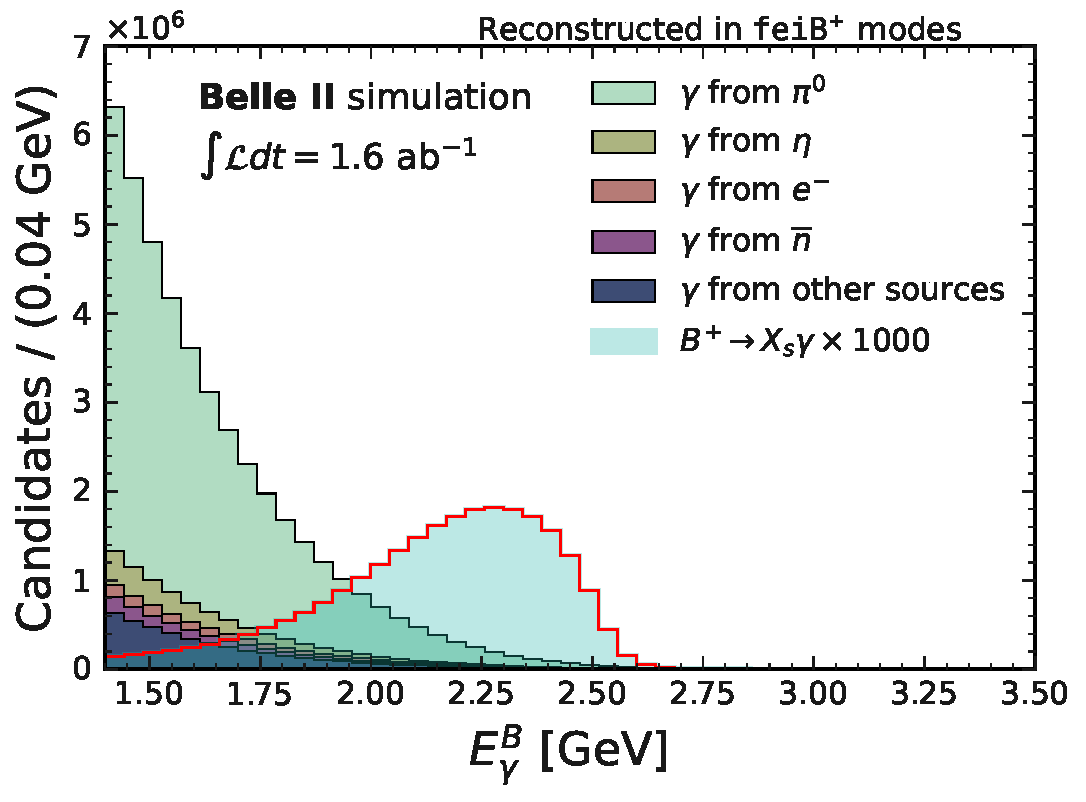
\includegraphics[width=0.45\textwidth]{figures/event_selection/Bp_photon_sources.pdf}
    }
    \subcaptionbox{\label{fig:bz_photon_sources}}{
        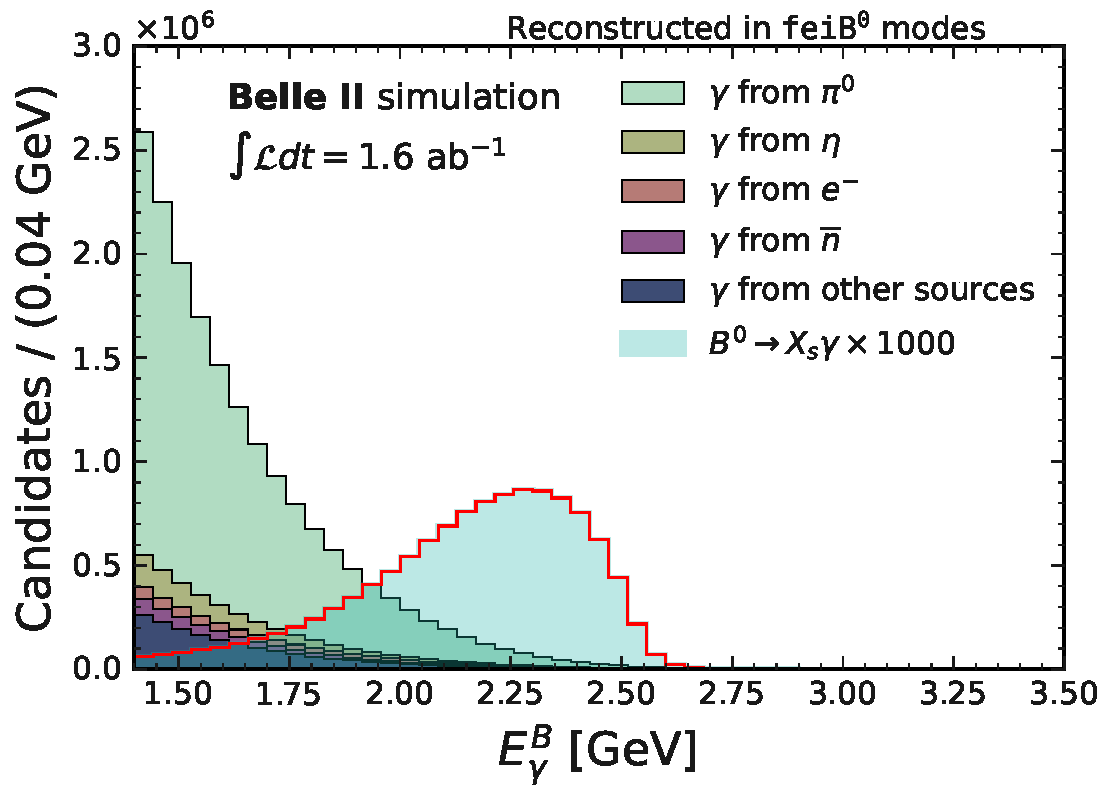
\includegraphics[width=0.45\textwidth]{figures/event_selection/Bz_photon_sources.pdf}
        }
    \caption{\label{fig:photon_sources} The background photon distribution after reconstruction in \feiBp and \feiBz modes, stacked by the photon mother-particle species.
    A scaled \BtoXsgamma spectrum is also overlaid.
    Only one photon candidate per event is shown, but it may still be paired with multiple tag-side candidates.
    Roughly 85\% of candidates originate in $\piz\ra\g\g$ or $\eta\ra\g\g$ decays.
    Other important backgrounds are photons from initial-state radiation, bremsstrahlung, and neutron-annihilation processes.
    These account for approximately 3\%, each.
    The leftover 10\% originate in various other decays.}
\end{figure}

At this stage, \BtoXsgamma events make up 0.05\% of the \feiBp sample and 0.07\% of the \feiBz sample.
To reduce the discussed background components the following strategy is adopted:
\begin{itemize}
    \item Suppress misidentified photons (different particle species);
    \item Suppress $\piz\ra\g\g$ and $\eta\ra\g\g$ decays;
    \item Suppress \epem\ra\qqbar events;
    \item Reoptimise all selections simultaneously to adopt a final set of selections.
\end{itemize}

\subsection{Misidentified photon suppression}\label{sec:selection_clusZMVA}

Neutrons, $K_L^0$, protons, electrons and other charged hadrons for which tracking for the particle did not succeed may leave clusters in the \ECL which are misidentified as photons.
The photon misidentification rate is given in \Cref{tab:misidentified_photons}.
The main misidentified photon candidates originate from neutrons with a small contribution from electron and $K_L^0$ showers.

\begin{table}[hbtp!]
    \centering
    \caption{\label{tab:misidentified_photons} Photon misidentification rates after reconstruction.
    The majority of photons are identified correctly. The largest component coming from misidentified neutron showers and $K_L^0$ deposits.
    The rates are similar for \feiBp and \feiBz modes which is consistent with the fact that this property is independent of the decaying $B$ charge.}
    \resizebox{1\textwidth}{!}{
\begin{tabular}{|l||c|c|c|c|c|c|c|c|c|c|c|}
    \hline
    Particle species & \multicolumn{2}{c|}{$\gamma$} & \multicolumn{2}{c|}{$n^0$} & \multicolumn{2}{c|}{$\en$} & \multicolumn{2}{c|}{$K_L^0$} & \multicolumn{2}{c|}{$p^-$} & Other \\
    \hline
    Candidate rate (\FEI \Bp | \Bz) & 96.1\% & 96.0\% & 2.4\% & 2.5\% & 0.5\% & 0.5\% & 0.5\% & 0.5\%  & 0.3\% & 0.3\% & 0.2\% \\
    \hline
\end{tabular}
}
\end{table}

Generally, the total energy deposit and distribution between \ECL crystals, also known as the \textit{shower shape}, is different depending on the particle species due to their different radiation lengths.
This can be used to distinguish photon clusters using \MVA methods.
A technique achieving this, which uses the moments of Zernike polynomials, is documented in Ref.~\cite{Hershenhorn:2468}.
This approach is implemented in \basftwo and used in this analysis.
Here, a condensed overview of the approach is provided.

A complete set of complex two-dimensional polynomials is defined as:
\begin{equation}
    V_{nm}(\rho\cos\alpha,\rho\sin\alpha) = R_{nm}(\rho)e^{im\alpha},
\end{equation}
where ${x=\rho\cos\alpha, y=\rho\sin\alpha}$ are polar coordinates, $m$ is an integer and $R_{nm}(\rho)=V(\rho,0)$ is a polynomial of degree $n$.
The expression for a Zernike polynomial is given as:
\begin{equation}
    R_{nm}(\rho) = \sum^{\frac{n-|m|}{2}}_{s=0}(-1)^s \frac{(n-s)!}{ s! \left(\frac{n+|m|}{2}-s \right) ! \left( \frac{n-|m|}{2}-s\right) !}\rho^{n-2s}.
\end{equation}
The moments of a function $f(\rho\cos\alpha,\rho\sin\alpha)$ are expressed in terms of $V_{nm}$ as:
\begin{equation}
    Z_{nm} = \frac{n+1}{\pi} \int_0^{2\pi}\int^1_0 V^*_{nm}(\rho\cos\alpha,\rho\sin\alpha)f(\rho\cos\alpha, \rho\sin\alpha)\rho d\rho d\alpha.
\end{equation}
$Z_{nm}$ are called Zernike moments.
They have many useful properties that make them usable in image recognition, the field of optics, and more importantly, particle identification algorithms (see. Ref.~\cite{Hershenhorn:2468} and references therein).

A Dirac comb is defined to parametrise a particle shower in the \ECL as:
\begin{equation}
    f(\vec{x}) = \sum_i \delta(\vec{x}-\vec{x}_i)\frac{w_iE_i}{\sum w_iE_i},
\end{equation}
where $\vec{x}$ is a dimensionless crystal position in the transverse plane, $i$ is a crystal index, summing over all crystals in a given particle shower, and $E_i$ is the energy of the $i$-th crystal.
As showers can overlap, $w_i$ is the fraction of energy in a crystal that is associated with the currently investigated shower.
It can be shown, that Zernike moments for \ECL showers can then be expressed as~\cite{Hershenhorn:2468}:
\begin{equation}
    |Z_{nm}| = \frac{n+1}{\pi}\frac{1}{\sum_iw_iE_i}\left|\sum_iR_{nm}(\rho_i)e^{-im\alpha_i}w_iE_i\right|.
\end{equation}

The work in Ref.~\cite{Hershenhorn:2468} selects the best combination of eleven $|Z_{nm}|$ which provides the strongest separation between hadronic showers and electromagnetic showers.
The chosen combination of $|Z_{nm}|$ is combined using a \BDT and produces a single output, hereafter referred to as $\ZMVA\in(0,1)$.
The \ZMVA distributions for \BtoXsgamma candidates in generic \MC and signal \MC events are shown in \Cref{fig:zmva_distribution}.

\begin{figure}[hbtp!]
    \centering
    \subcaptionbox{\label{fig:bp_zmva_distribution}}{
        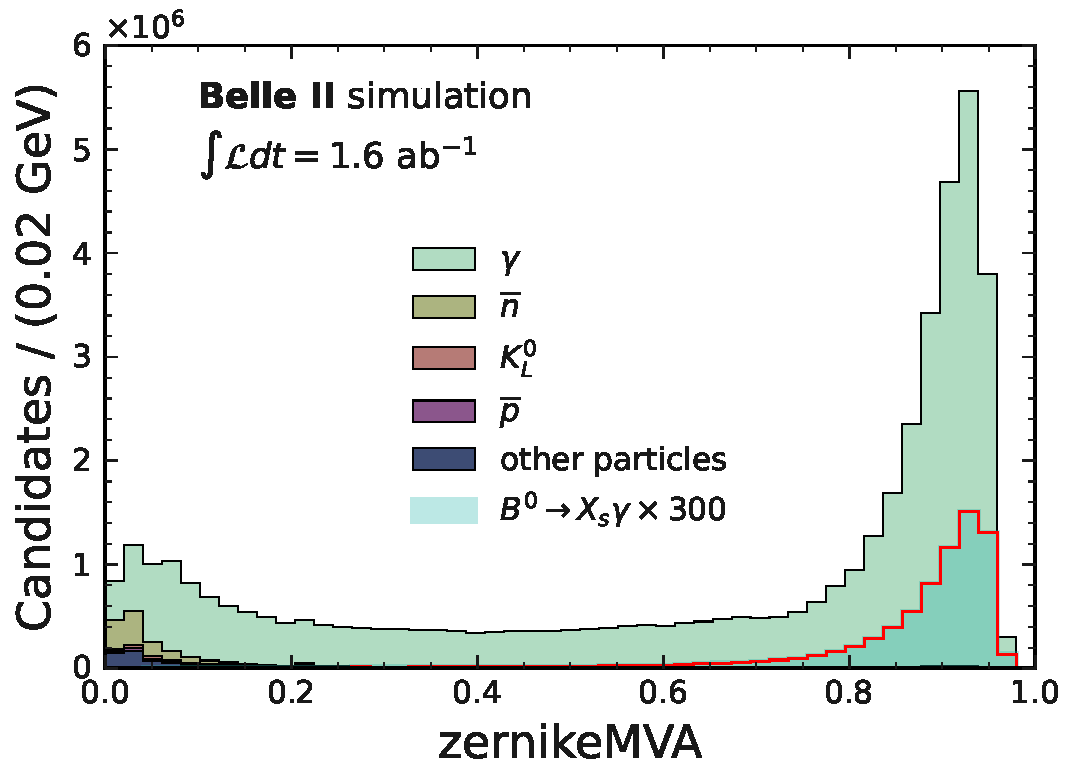
\includegraphics[width=0.45\textwidth]{figures/event_selection/Bp_zernikeMVA_mcPDG.pdf}
    }
    \subcaptionbox{\label{fig:bz_zmva_distribution}}{
        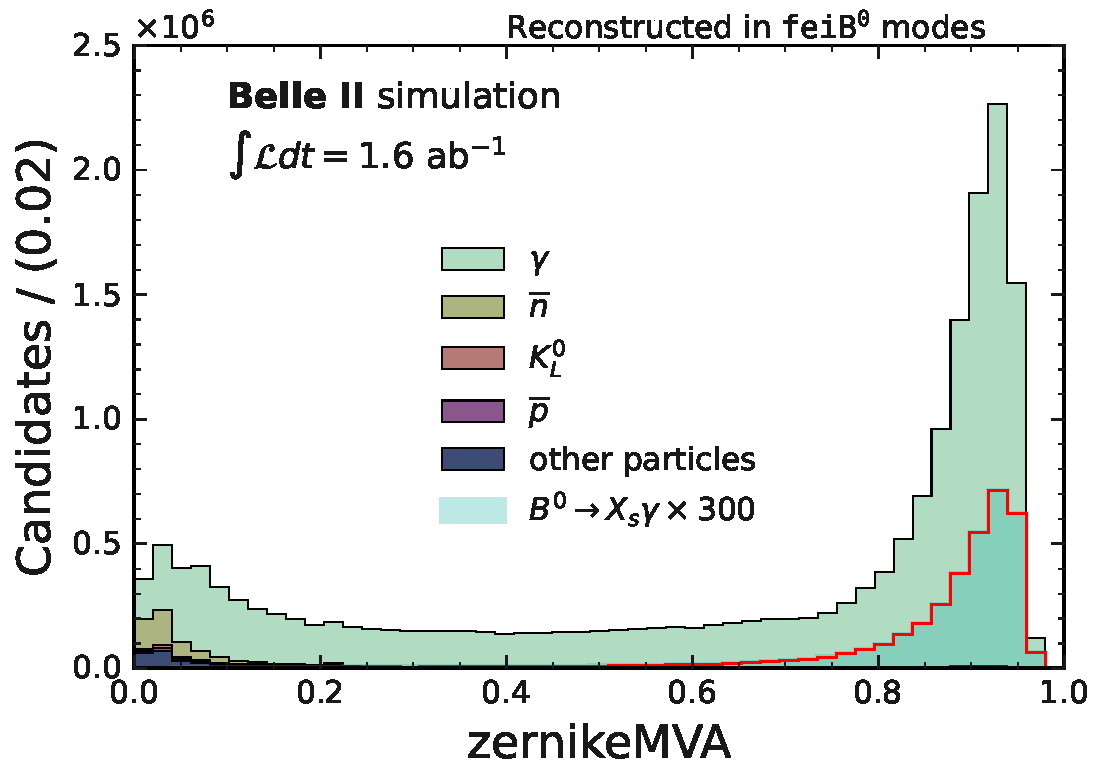
\includegraphics[width=0.45\textwidth]{figures/event_selection/Bz_zernikeMVA_mcPDG.pdf}
        }
    \caption{\label{fig:zmva_distribution} The distributions of the \ZMVA for different particle species that are reconstructed as photon candidates in \feiBp and \feiBz modes.
    The candidates presented in these Figures are the same as those in \Cref{fig:photon_sources}.
    A scaled \ZMVA distribution for \BtoXsgamma events is overlaid.
    A good separation is observed between real photons and hadronic showers misidentified as photons.}
\end{figure}

Overall, for true photons this distribution is strongly peaking in the $0.8-1$ region.
Misidentified hadrons peak close to 0.
For non-\BtoXsgamma photon candidates, this distribution remains relatively uniform in the $0-0.8$ region.
Moreover, \ZMVA provides a good separation against real photon candidates that originate in neutron annihilation events.
This is shown by a \ZMVA distribution exclusively for true photon candidates in \Cref{fig:zmva_distribution_sources}.

\begin{figure}[hbtp!]
    \centering
    \subcaptionbox{\label{fig:bp_zmva_distribution_sources}}{
        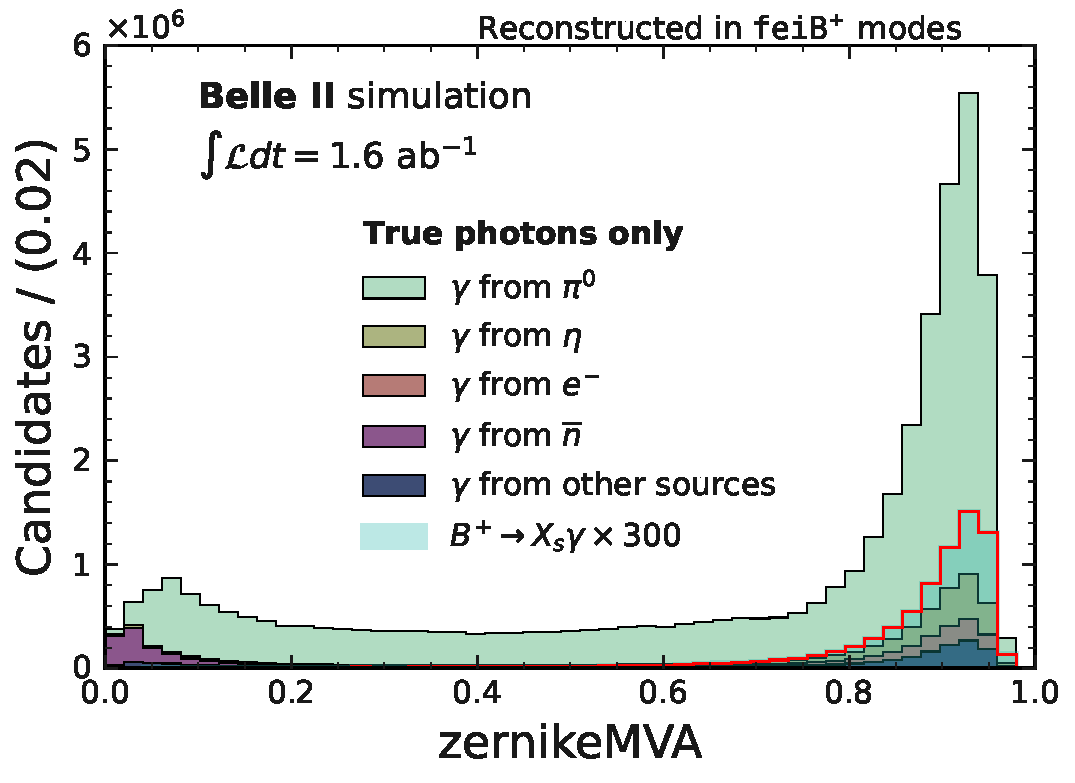
\includegraphics[width=0.45\textwidth]{figures/event_selection/Bp_zernikeMVA_true_photons_only.pdf}
    }
    \subcaptionbox{\label{fig:bz_zmva_distribution_sources}}{
        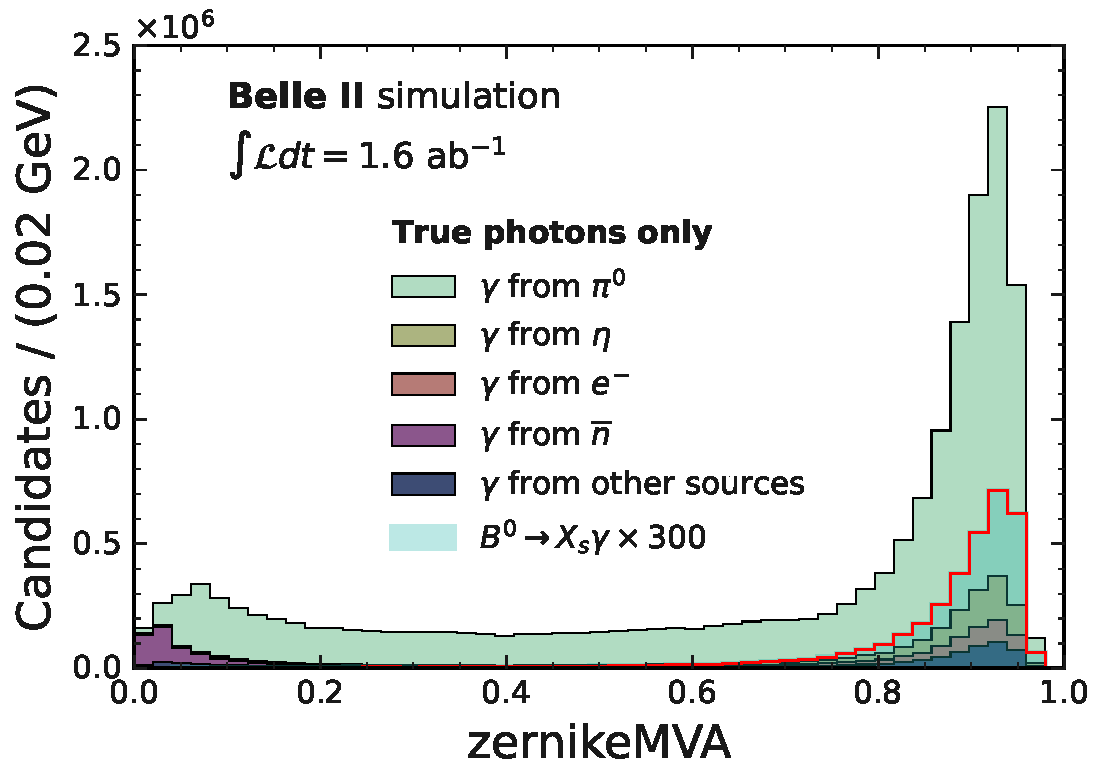
\includegraphics[width=0.45\textwidth]{figures/event_selection/Bz_zernikeMVA_true_photons_only.pdf}
        }
    \caption{\label{fig:zmva_distribution_sources} The distributions of the \ZMVA for different photon sources in generic \MC reconstructed in \feiBp and \feiBz modes.
    The candidates presented here are only those which are true photons in \Cref{fig:zmva_distribution}.
    A scaled \ZMVA distribution for \BtoXsgamma events is overlaid.
    Photons associated with neutron annihilation events are separated.}
\end{figure}

\subsection{Suppression of \texorpdfstring{\piz}{pi0} and \texorpdfstring{$\eta$}{eta} diphoton decays}\label{sec:selection_vetos}

Aboout 85\% of background photons in this analysis originate from photons that are produced in $\piz\ra\g\g$ or $\eta\ra\g\g$ decays.
A lot of such light mesons originate in continuum events, but they are prominent even in \BB events.
Therefore, an efficient mechanism to suppress \piz- and $\eta$-related photon candidates is required.

In this analysis, a suppression tool, called \textit{\piz~and~\eta~veto} is utilised.
It is implemented as part of \basftwo and is a standard Belle~II approach for suppression of radiative backgrounds from light mesons.
Here, an overview of the training and the validation process is provided which is performed by an independent analysis.

The general idea of the \piz~and~\eta~veto is to pair the high energy photon signal candidate (\textit{hard} photon) with lower energy photons (\textit{soft} photons) in the event.
The compatibility of the combination with a $\piz\ra\g\g$ or $\eta\ra\g\g$ decay is evaluated and a probability-like quantity is calculated to quantify it.

The soft photon candidate is selected with an energy of $30~\mev$ ($40~\mev$ in the backward \ECL endcap) for $\piz$ or $60~\mev$ for $\eta$.
The photon is also required to have deposited the energy in two or more crystals.
Furthermore, photon candidates are required to have an associated cluster time less than one standard deviation away from zero.
These selections ensure that beam background photons, neutral hadrons misidentified as photons and misreconstructed charged particles are not included in the soft photon sample.

The soft photons that pass these selections are combined with the hard photon candidate.
The following observables are then calculated and used to train a \MVA classifier:
\begin{itemize}
    \item Invariant mass of the soft photon and hard photon combination;
    \item Soft photon energy in the laboratory frame;
    \item Soft photon \ECL cluster polar angle;
    \item Distance between the soft photon \ECL cluster and the nearest track extrapolated to the \ECL;
    \item Helicity angle of the combination.
\end{itemize}
The classifier for $\eta\ra\g\g$ includes additional observables to increase the separation power:
\begin{itemize}
    \item \ZMVA of the soft photon;
    \item Number of crystals where the soft photon has deposited energy;
    \item Ratio of soft photon energy in 3-by-3 crystals around the central crystal to soft photon energy in the 5-by-5 crystals with the corner crystals removed.
\end{itemize}
For every combination of a soft and hard photon, the \MVA produces an output between 0 and 1.
The same hard photon is paired with all soft photons in a given event, and the largest \MVA output is assigned to it as the $\piz$ or $\eta$ probability.
This \MVA output is denoted as \piVeto or \etaVeto, respectively.
Note that despite the nomenclature, this variable is only probability-like (i.e. $\mathcal{P}\in(0,1)$) but does not truly represent a probability.
The distributions for \piVeto and \etaVeto are shown in \Cref{fig:vetos}.
In all cases, \BtoXsgamma can be seen to be strongly peaking near 0, consistent with photons that do not originate from light unflavoured meson decays.

\begin{figure}[hbtp!]
    \centering
    \subcaptionbox{\label{fig:bp_piveto}}{
        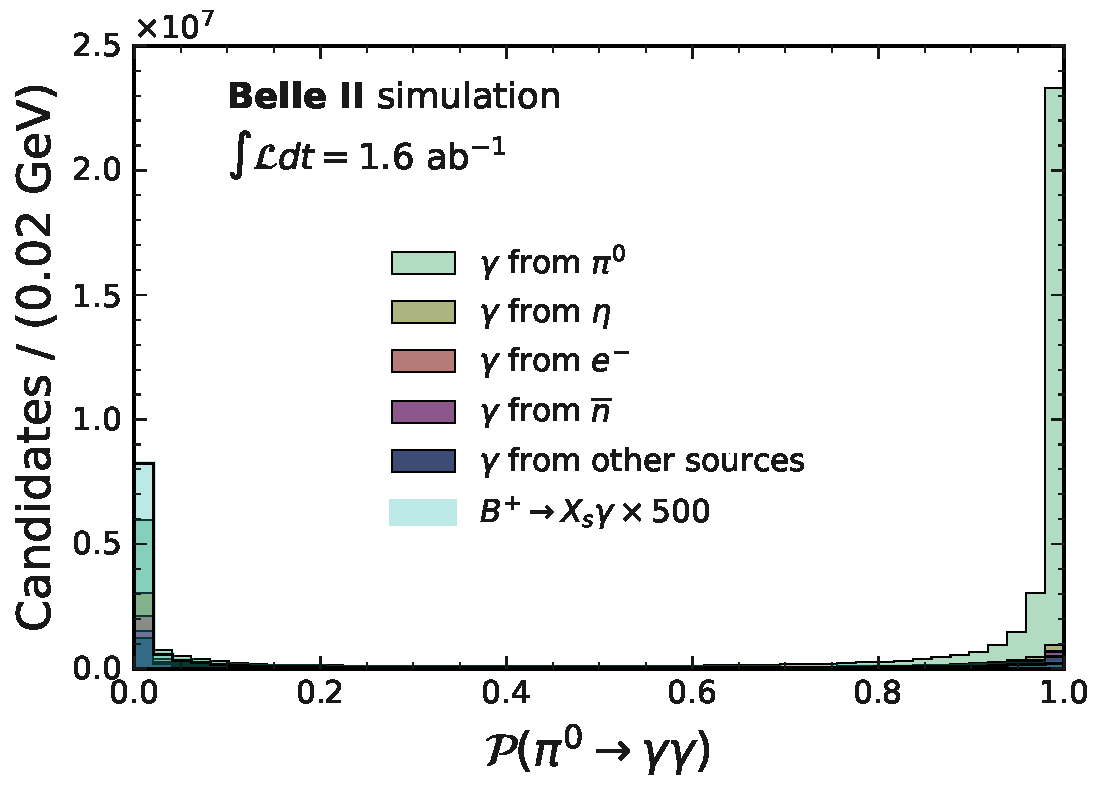
\includegraphics[width=0.45\textwidth]{figures/event_selection/Bp_piVeto.pdf}
        }
    \subcaptionbox{\label{fig:bz_piveto}}{
        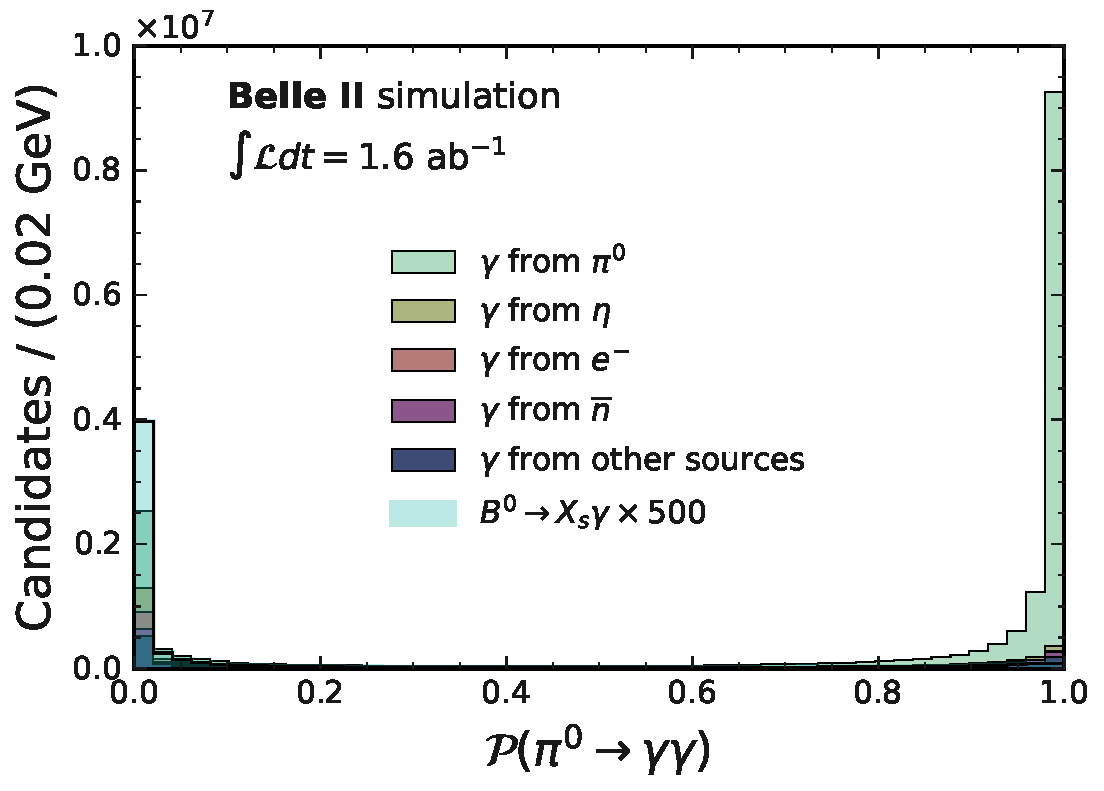
\includegraphics[width=0.45\textwidth]{figures/event_selection/Bz_piVeto.pdf}
        }
    \subcaptionbox{\label{fig:bp_etaveto}}{
            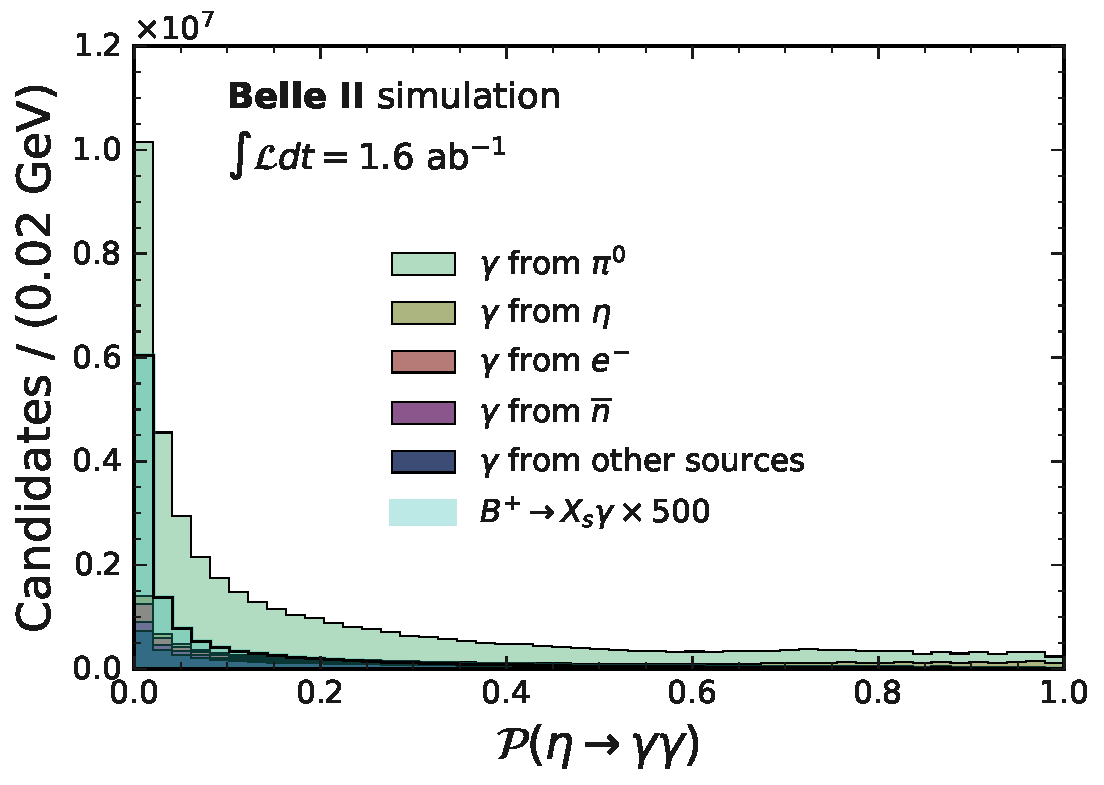
\includegraphics[width=0.45\textwidth]{figures/event_selection/Bp_etaVeto.pdf}
        }
    \subcaptionbox{\label{fig:bz_etaveto}}{
            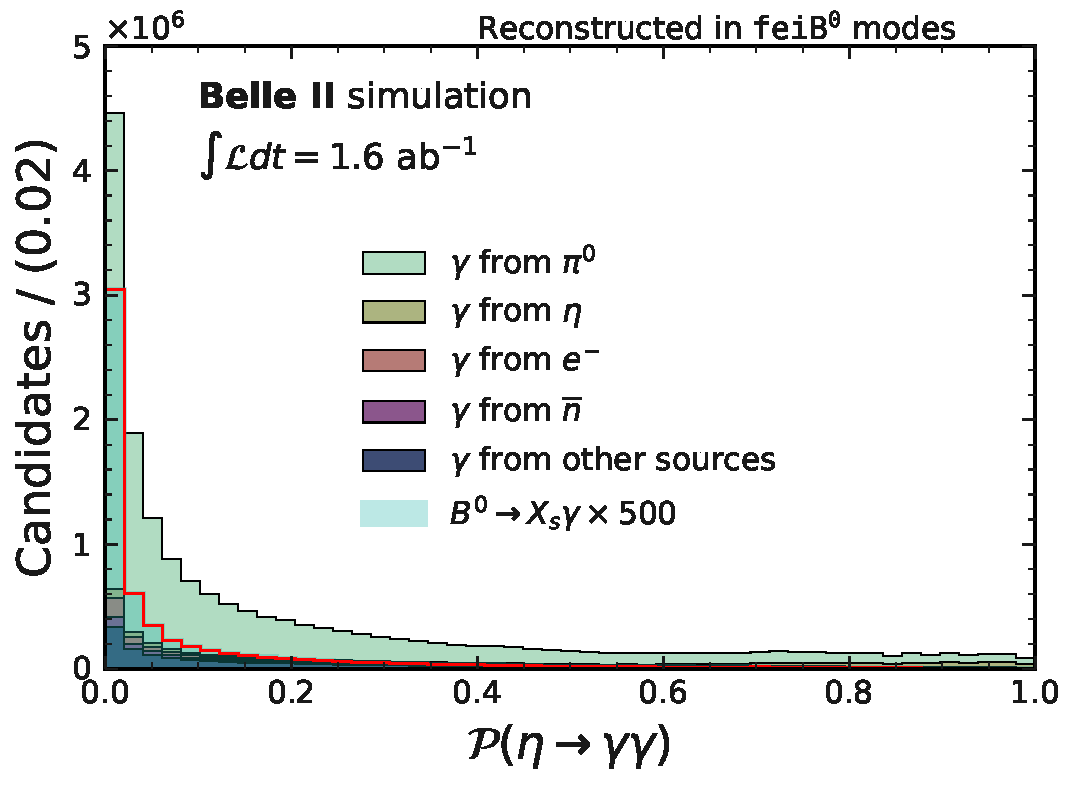
\includegraphics[width=0.45\textwidth]{figures/event_selection/Bz_etaVeto.pdf}
        }
    \caption{\label{fig:vetos} 
    The distributions of \piVeto ((\subref{fig:bp_piveto}) and (\subref{fig:bz_piveto})) 
    and \etaVeto ((\subref{fig:bp_etaveto}) and (\subref{fig:bz_etaveto}))
    for different photon sources in generic \MC reconstructed in \feiBp and \feiBz modes.
    This is shown for all photon candidates included in \Cref{fig:photon_sources}.
    Scaled respective veto probability distributions for \BtoXsgamma events are overlaid.
    The separation power of \etaVeto is hidden by a large number of $\piz\ra\g\g$ events in (\subref{fig:bp_etaveto}) and (\subref{fig:bz_etaveto}).
    It is apparent again when \piz decays events are removed from the sample as shown in \Cref{fig:vetos_nopi}.
    }
\end{figure}

For the case of \piz veto, shown in \Cref{fig:bp_piveto,fig:bz_piveto}, an excellent separation is observed between photons originating in \piz decays and other photons.
\BtoXsgamma and other non-\piz photon candidates also show a small peak at high-\piVeto values, which alludes to a small inefficiency of the algorithm.
However, compared to the separation power provided, this is an acceptable trade-off.
For the \etaVeto, the separation is less clear.
The reason for this is the fact that the generic \MC sample is dominated by $\piz\ra\g\g$ decays which are not targeted by the \etaVeto classifier.
Removing $\piz\ra\g\g$ decays from the sample, a clear separation of photon candidates originating in $\eta$ decays from other types of decays becomes apparent (see \Cref{fig:vetos_nopi}).

\begin{figure}[hbtp!]
    \centering
    \subcaptionbox{\label{fig:bp_etaveto_nopi}}{
            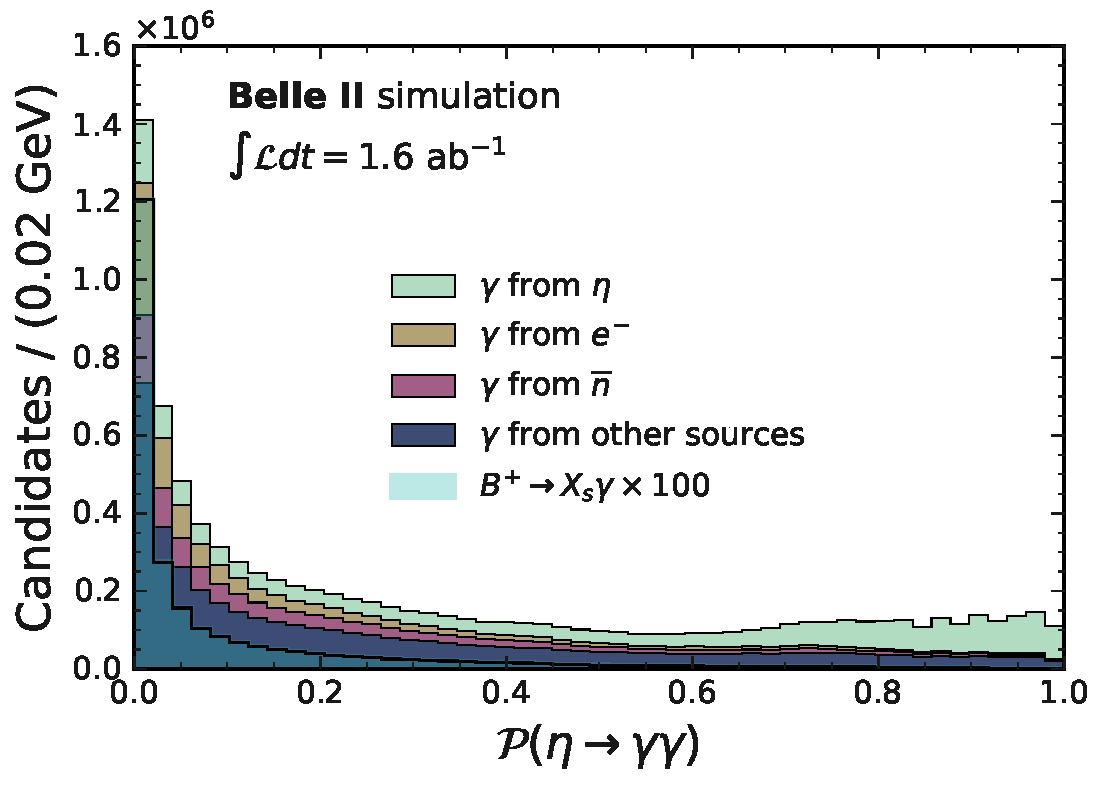
\includegraphics[width=0.45\textwidth]{figures/event_selection/Bp_etaVeto_nopi.pdf}
        }
    \subcaptionbox{\label{fig:bz_etaveto_nopi}}{
            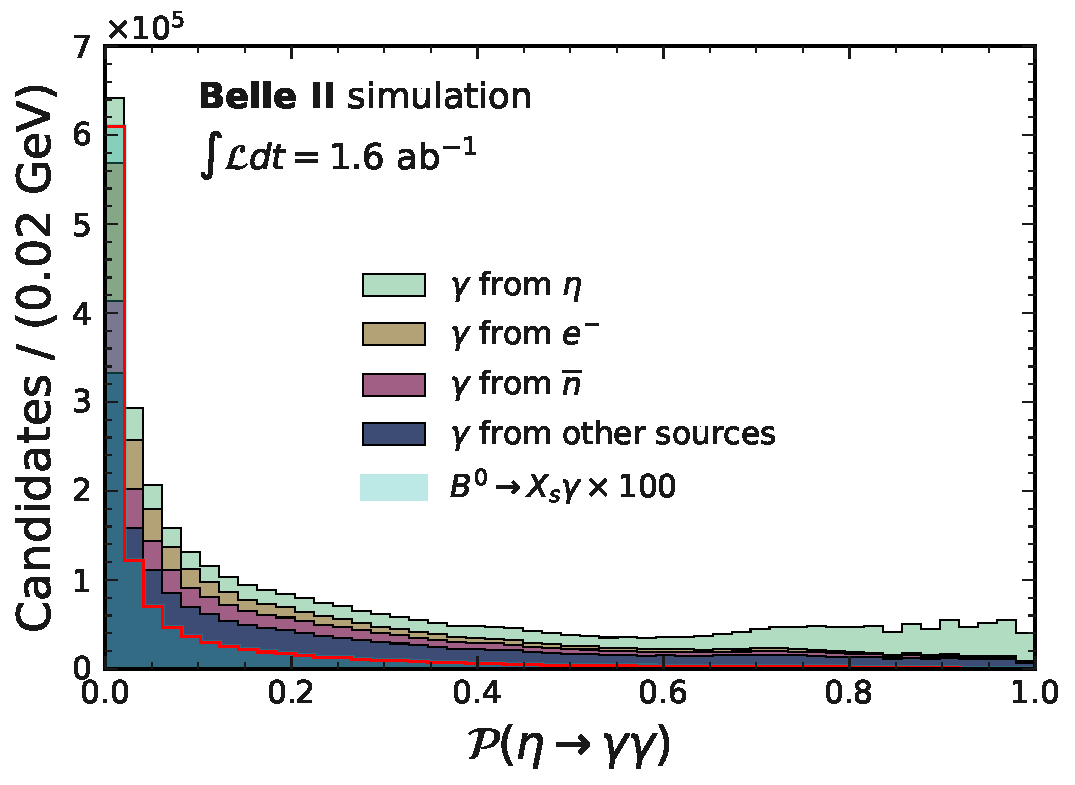
\includegraphics[width=0.45\textwidth]{figures/event_selection/Bz_etaVeto_nopi.pdf}
        }
    \caption{\label{fig:vetos_nopi} The distributions of \etaVeto
    for different photon sources in generic \MC reconstructed in \feiBp and \feiBz, but with photons that are associated with $\piz\ra\g\g$ removed.
    This is equivalent to \Cref{fig:bp_etaveto,fig:bz_etaveto} with the \piz component not included.
    A scaled \etaVeto distribution for \BtoXsgamma events is overlaid.
    Although the separation power is not as strong as in the case of \piVeto (\Cref{fig:bp_piveto,fig:bz_piveto}), a clear peak at low-\etaVeto can be seen for \BtoXsgamma.
    }
\end{figure}

\subsection{Signal-photon background suppression correlation}\label{sec:signal_photon_correlation}

Even though no direct selection is applied on the $X_s$ system, through direct or higher-order correlations with \EB, a bias may be introduced to the photon energy.
To ensure that no such effect is introduced, a correlation study is performed for \piVeto, \etaVeto and \ZMVA observables.
In principle, it is acceptable if the selection introduces a bias to the background, as long as this bias is well reproduced in simulation.
The latter will be validated in \Cref{sec:corrections,sec:signal_modelling}.
Therefore, the study is performed exclusively focusing on \BtoXsgamma events, as it is aimed to ensure that the photon energy spectrum itself is minimally biased.

\begin{figure}[hbtp!]
    \centering
    \subcaptionbox{\label{fig:bp_zmva_correlation}}{
            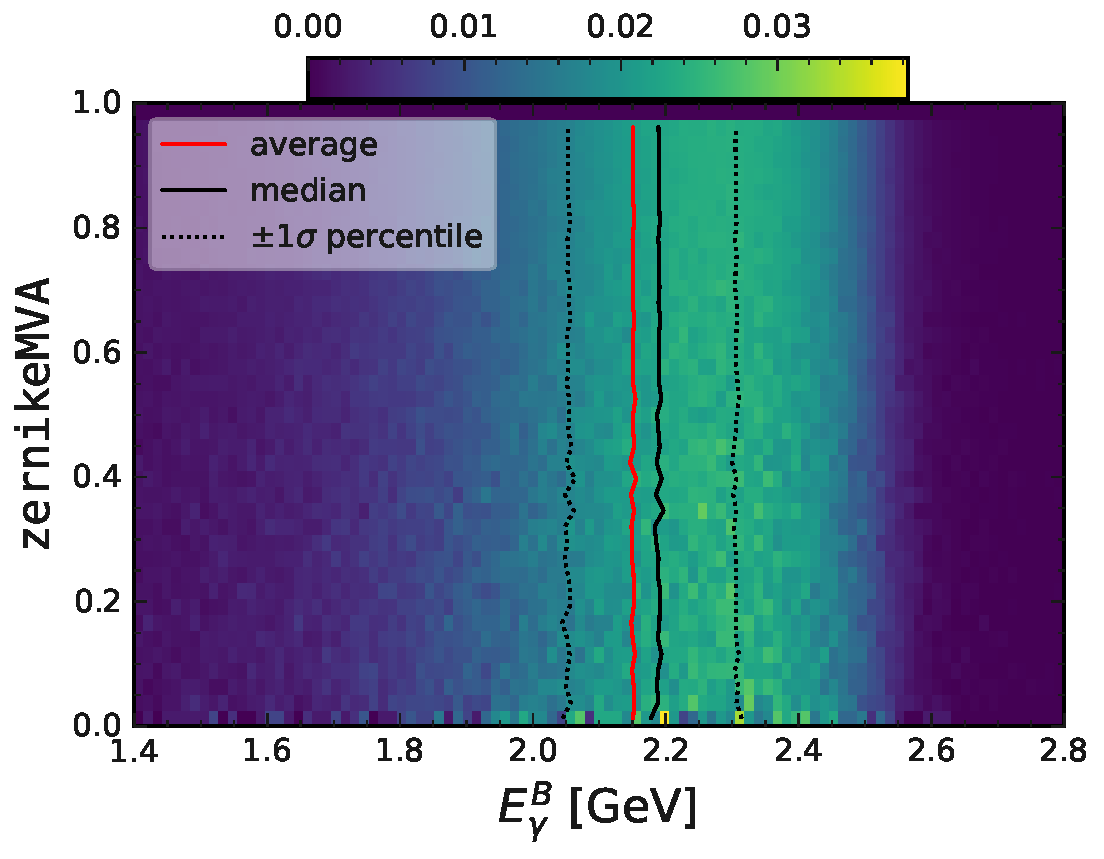
\includegraphics[width=0.31\textwidth]{figures/event_selection/Bp_zernikeMVA_correlation.pdf}
    }
    \subcaptionbox{\label{fig:bp_piveto_correlation}}{
            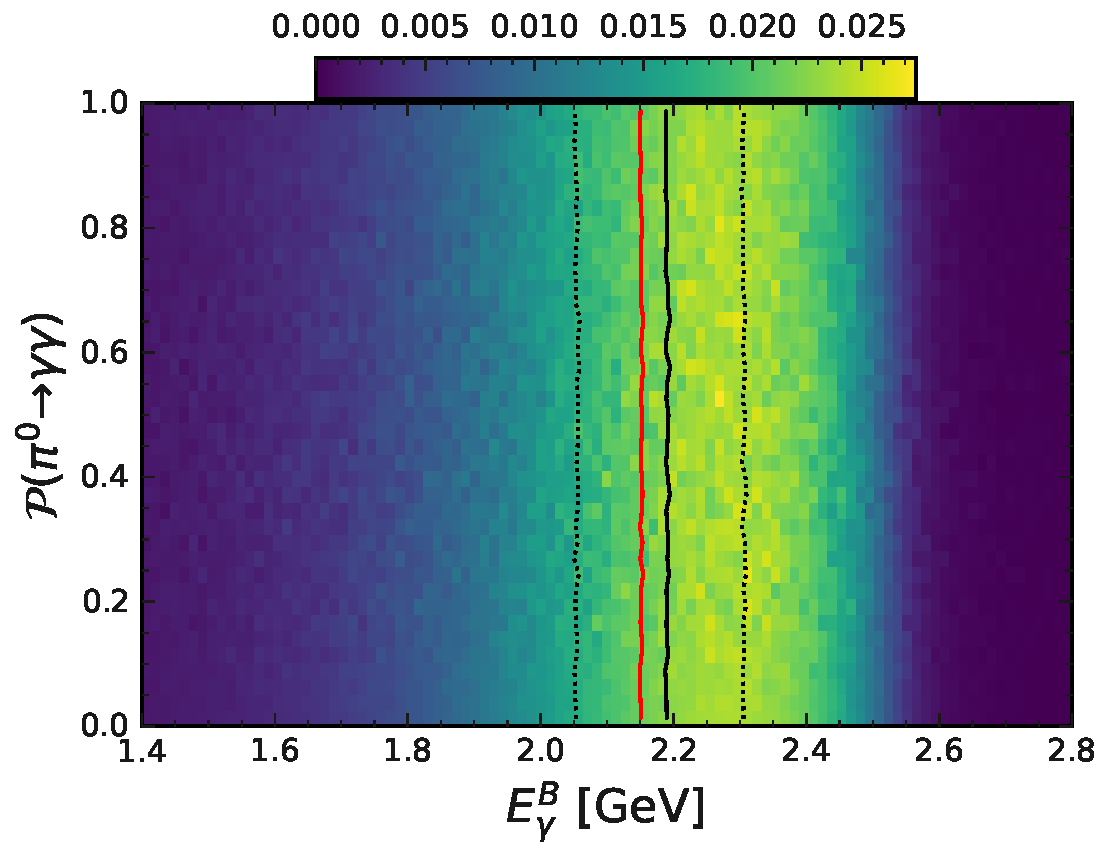
\includegraphics[width=0.31\textwidth]{figures/event_selection/Bp_piVeto_correlation.pdf}
    }
    \subcaptionbox{\label{fig:bp_etaveto_correlation}}{
        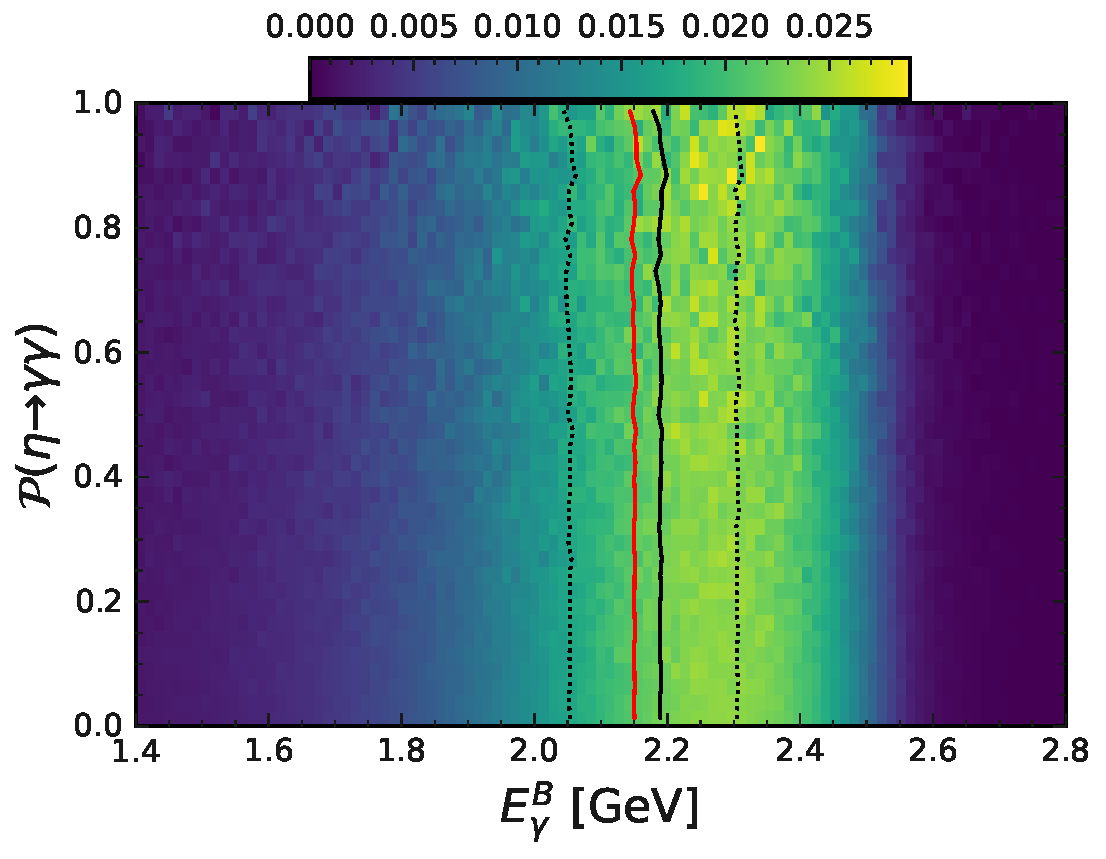
\includegraphics[width=0.31\textwidth]{figures/event_selection/Bp_etaVeto_correlation.pdf}
    }
    \subcaptionbox{\label{fig:bz_zmva_correlation}}{
            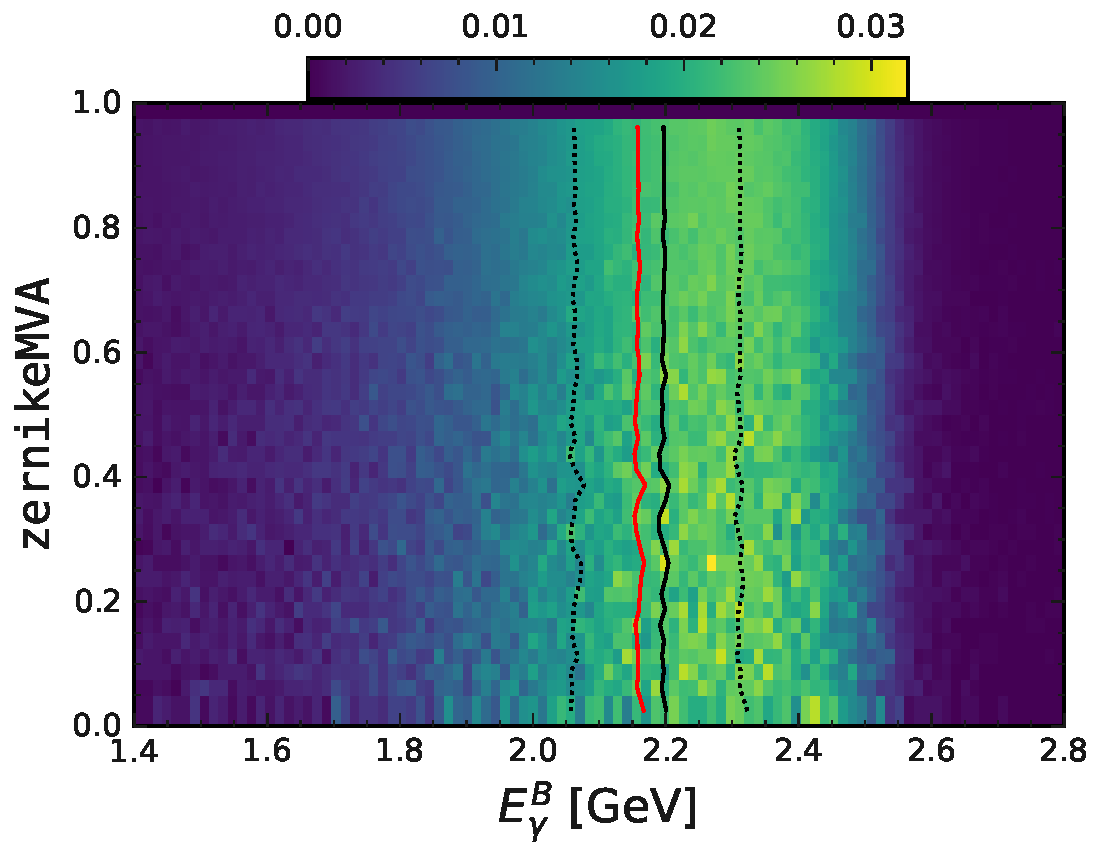
\includegraphics[width=0.31\textwidth]{figures/event_selection/Bz_zernikeMVA_correlation.pdf}
    }
    \subcaptionbox{\label{fig:bz_piveto_correlation}}{
            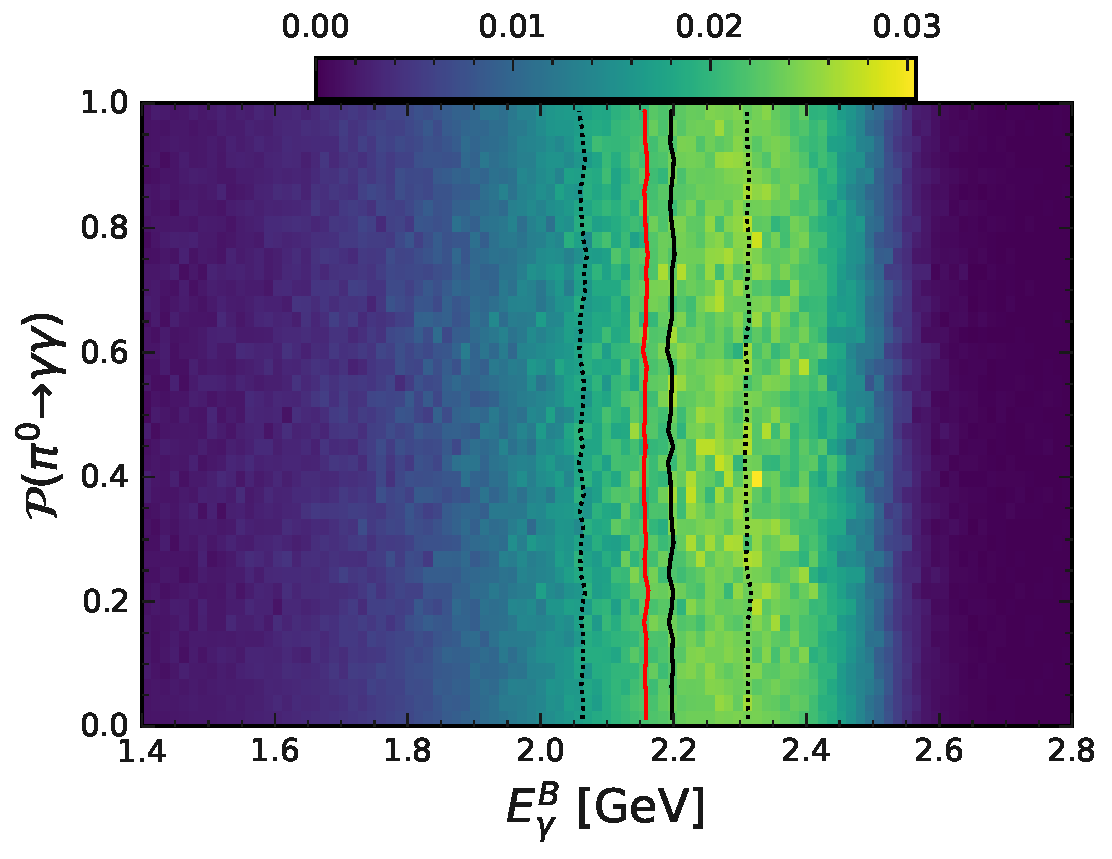
\includegraphics[width=0.31\textwidth]{figures/event_selection/Bz_piVeto_correlation.pdf}
    }
    \subcaptionbox{\label{fig:bz_etaveto_correlation}}{
            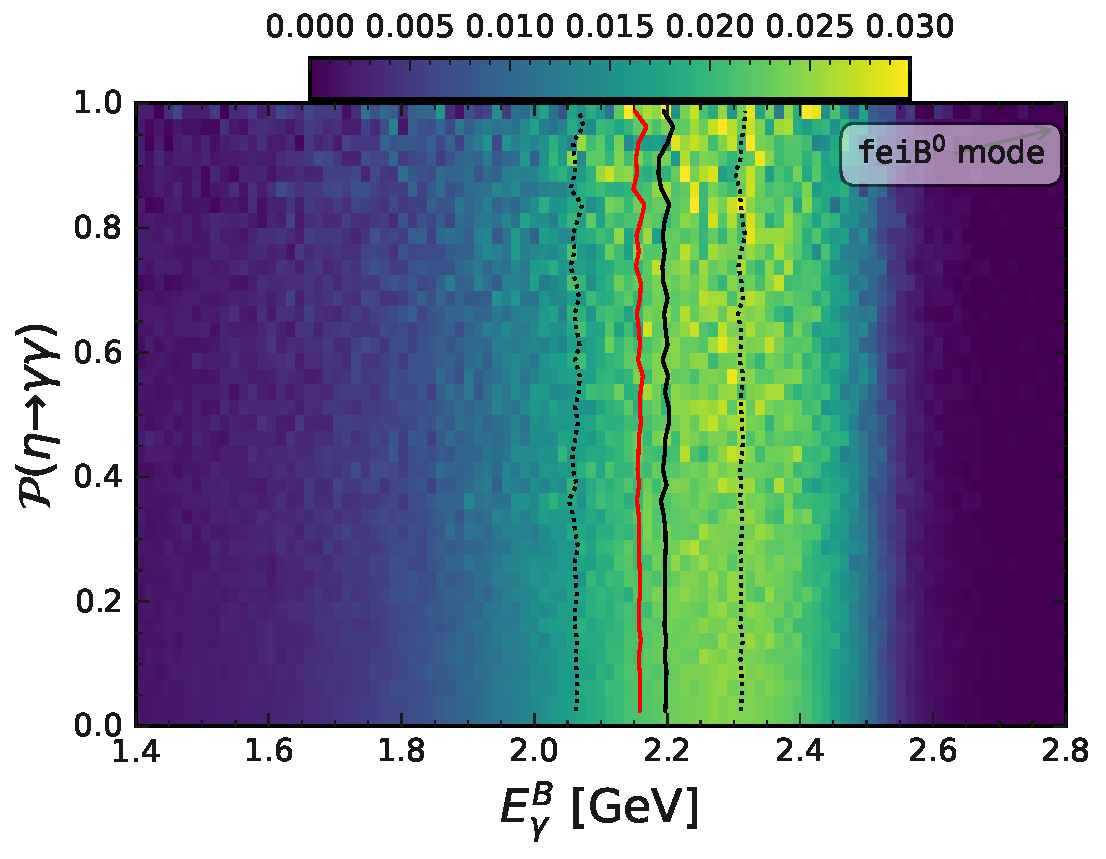
\includegraphics[width=0.31\textwidth]{figures/event_selection/Bz_etaVeto_correlation.pdf}
    }
    \caption{\label{fig:selection_correlations} Correlation tests for background suppression observables described in \Cref{sec:photon_selection}, depicted as a 2D histogram.
    Each row is normalised such that all bins within that row add up to 1.
    For signal \BptoXsgamma events, the tests are shown
    in the upper panels \mbox{(\subref{fig:bp_zmva_correlation}) -- (\subref{fig:bp_etaveto_correlation})},
    and for \BztoXsgamma in the lower ones \mbox{(\subref{fig:bz_zmva_correlation}) -- (\subref{fig:bz_etaveto_correlation})}.
    In the red line, the average photon energy, $\expval**{\EB}$, is shown as a function of the tested observable.
    In black and black-dotted lines: the median and $\pm 1 \sigma$ percentile values of \EB, respectively.
    No strong dependence can be observed in any of the quantities or the 2D maps.
    }
\end{figure}

A two-dimensional map of ${\piVeto,\etaVeto,\ZMVA}$ versus \EB is given in \Cref{fig:selection_correlations}.
Because the distributions of the three variables used for background suppression are not uniform, each row is normalised such that the sum of each row is equal to unity.
This makes the comparison between differently populated bins simpler.
The Figure also denotes the average, the median and $\pm 1\sigma$ percentiles of \EB.
No strong bias is introduced by any of the observables to any of these quantities.
Furthermore, the structure itself remains constant across all bins and no clear dependence on \EB can be seen.
No significant differences between different \FEI modes are observed.
It is therefore concluded that the selections are unbiasing and suitable for signal-side photon background suppression.
The exact selections on these observables are optimised simultaneously with continuum event suppression in \Cref{sec:final_optimisation}.

\section{\texorpdfstring{\MakeLowercase{\epem\ra\qqbar}}{e+e-->qqbar} event suppression}\label{sec:continuum_suppression}
\Cref{sec:photon_selection} introduced the best-photon candidate strategy, 
as well as selection to suppress events 
where the photon is misidentified or originates in sources different from \BtoXsgamma.
However, as was seen before in, for example, \Cref{fig:spectrum_after_reco},
\epem\ra\qqbar events provide the vast majority of photon candidates.
Therefore, a dedicated event-selection for this type of background was devised.
It takes advantage of  different event topologies expected for $\FourS\to\qqbar$ and $\epem\ra\qqbar$ events.
Loosely speaking, events where a $\FourS\to\BB$ decay is present tend to be more `spherical', when compared with $\epem\ra\qqbar$ events that exhibit a `jet-like' distribution.
This is related to the fact that \epem collisions at $B$ factory experiments have just enough energy to produce a $B$ pair almost at rest, which means that its decays products, on average, tend to be distributed uniformly in polar and azimuthal angle.
On the other hand, light-quark pairs, produced in \epem collision events, also gain a substantial amount of back-to-back momentum which tends to spread their decay products. 
The schematic idea of this is shown in \Cref{fig:continuum_schematic}.
This section will provide an in-depth discussion on how the discrimination between \BtoXsgamma and continuum is achieved using a \BDT.

\begin{figure}[htbp!]
    \centering
    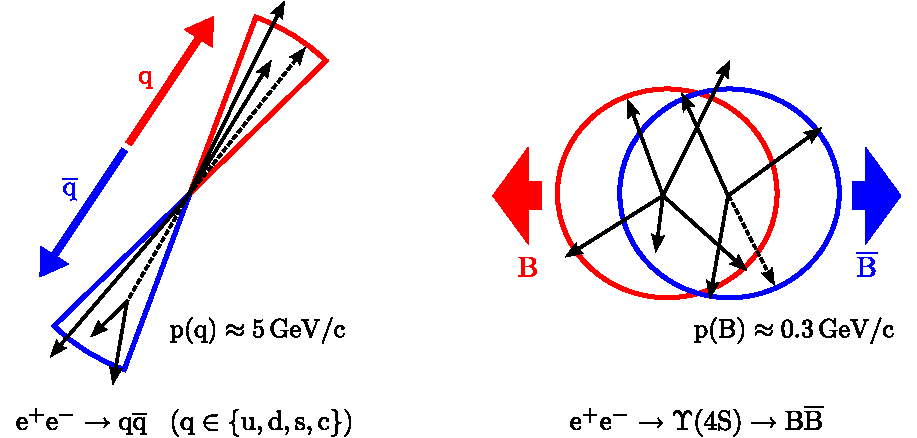
\includegraphics[width=0.6\textwidth]{figures/continuum_suppression/figure_continuum_suppression_event_shapes.pdf}
    \caption{\label{fig:continuum_schematic} Schematic illustration of continuum and \BB events created after an \epem collision in $B$ factories.
    Events where a $B$ meson is produced are generally more spherical, due to the fact that \FourS is produced at rest and its decays products tend to not have a preferred direction.
    Typical momenta of light-quark and \BB mesons are shown.
    The specific directions shown are illustrative only. 
    }
\end{figure}

\subsection{Training event pre-selection}\label{sec:preselection}

Before a \BDT is trained, it is generally desirable to prepare the datasets such that the classifier 
is able to learn based on relevant data.
Such data preprocessing will be performed based on variables described in \Cref{sec:photon_selection}.
The classifier will then be trained on the reduced dataset

In order to find optimal selections, a figure-of-merit study is performed for each observable.
Two figure-of-merit options were considered for this analysis, a more standard figure-of-merit $\mathrm{FOM}_1$:
\begin{equation}\label{eq:soversqrtsplusb}
    \mathrm{FOM}_1 = \frac{\mathsf{S}}{\sqrt{\mathsf{S}+\mathsf{B}}},
\end{equation}
and $\mathrm{FOM}_2$ defined in Ref.\cite{Punzi:2003bu} (often referred to as `Punzi' figure-of-merit):
\begin{equation}\label{eq:punzi_fom}
    \mathrm{FOM}_2 = \frac{\mathsf{S}}{\mathsf{S}_0} \frac{1}{\frac{3}{2}+\sqrt{\mathsf{B}}}.
\end{equation}
In both equations, $\mathsf{S}$ is the number of signal events after selection, 
$\mathsf{B}$ is the number of background events after selection, 
and $\mathsf{S}_0$ is the number of signal events before selection.
Although \Cref{eq:punzi_fom} was derived with search-like analyses in mind, 
it is utilised in this analysis to minimise signal model dependency: the ratio $\mathsf{S}/\mathsf{S}_0$ present in the definition reduces out many model-dependant effects.

For each figure of merit calculation, background events ($\mathsf{B}$) are calculated based on generic \MC,
whereas signal events, $\mathsf{S}$, are calculated based on signal \MC, to ensure a high statistics sample.
In the case of \Cref{eq:soversqrtsplusb}, an appropriate scaling for $\mathsf{S}$ is also used.
Each dataset has duplicate tag-candidate events randomly removed, by picking a random tag-side candidate.
Each figure of merit is then calculated for 200 equally spaced selections in the target observable.
The maximum figure-of-merit point is taken as the optimal pre-selection for each of the variables.
This procedure is shown for $\mathrm{FOM}_2$ in \Cref{fig:selection_optimisations}.
Results for $\mathrm{FOM}_1$ are used as a cross-check for $\mathrm{FOM_2}$ but turn out to be consistent.
Equivalent procedure for $\mathrm{FOM}_1$ is shown in \Cref{sec:appendix_sqrtsplusb_optimisation}.
The resulting optimal selections are also shown in the Figures.

\begin{figure}[htbp!]
    \centering
    \subcaptionbox{\label{fig:bp_zmva_optimisation}}{
            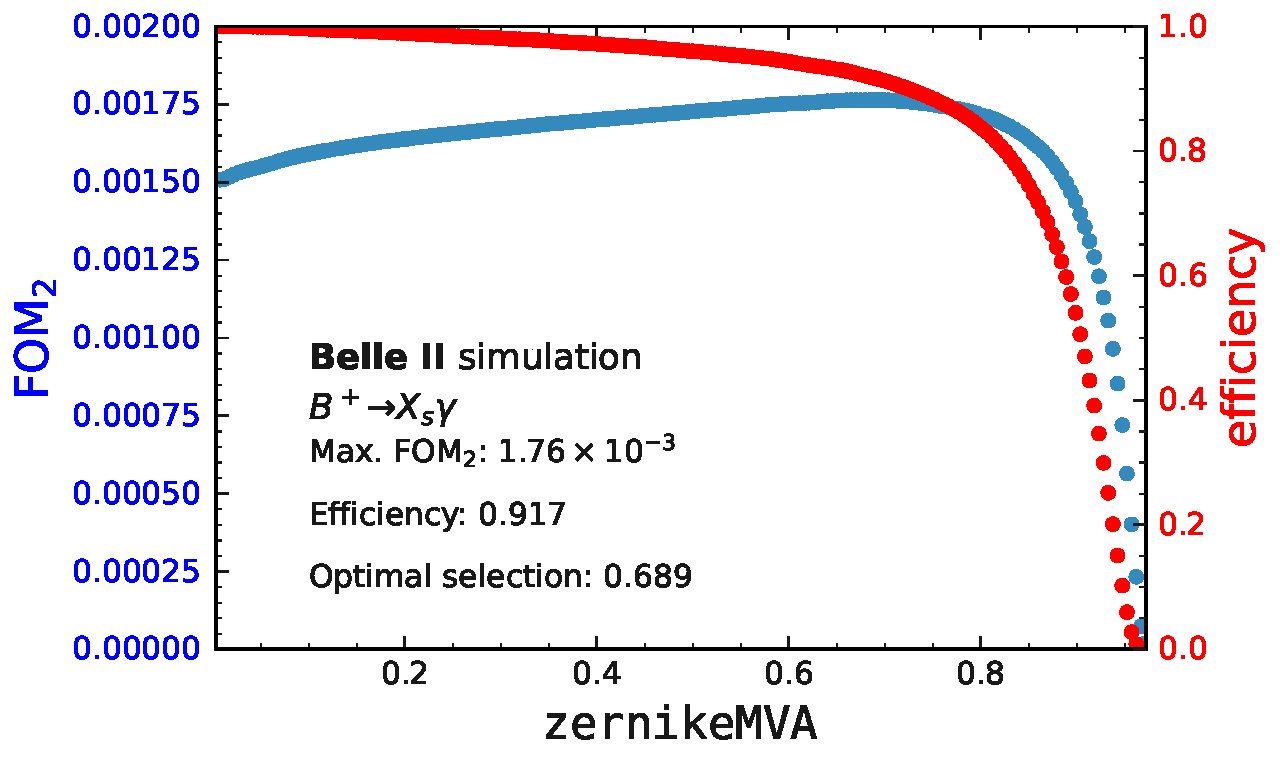
\includegraphics[width=0.3\textwidth]{figures/continuum_suppression/Bp_zernikeMVA_optimisation_punzi.pdf}
        }
    \subcaptionbox{\label{fig:bp_piveto_optimisation}}{
            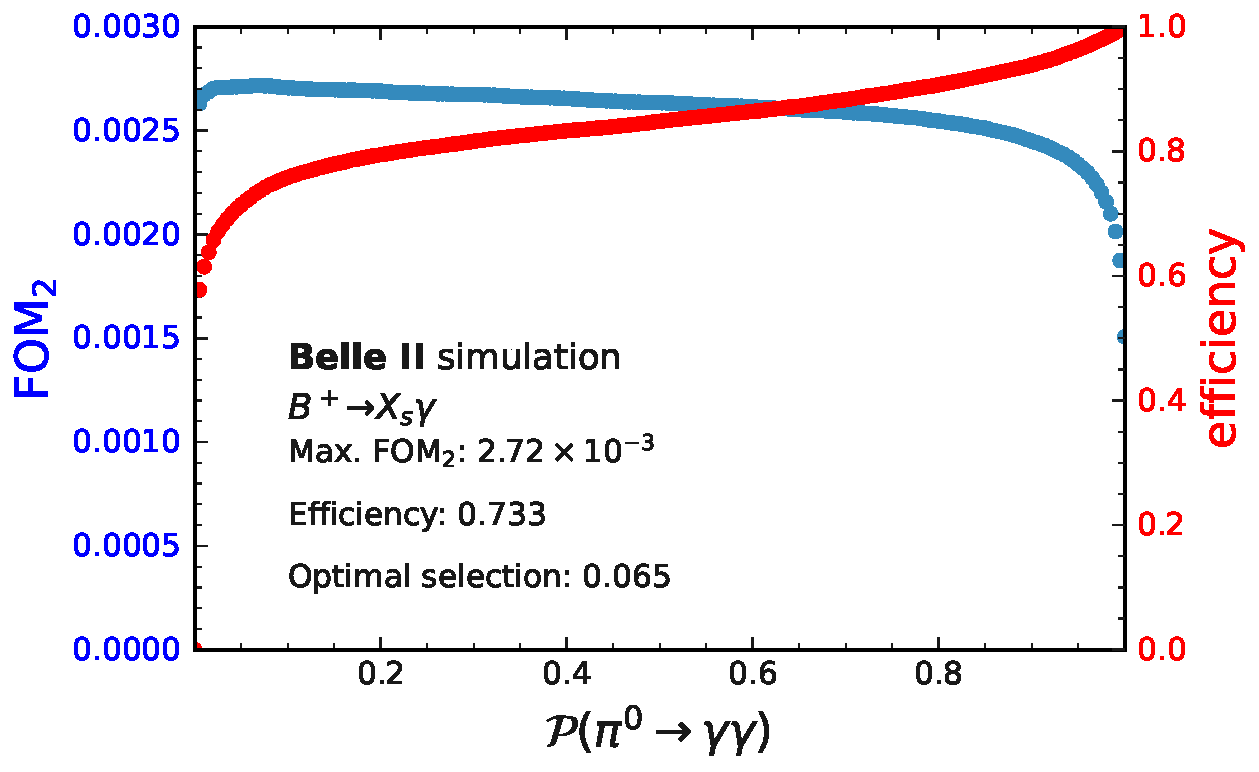
\includegraphics[width=0.3\textwidth]{figures/continuum_suppression/Bp_piVeto_optimisation_punzi.pdf}
        }
    \subcaptionbox{\label{fig:bp_etaveto_optimisation}}{
            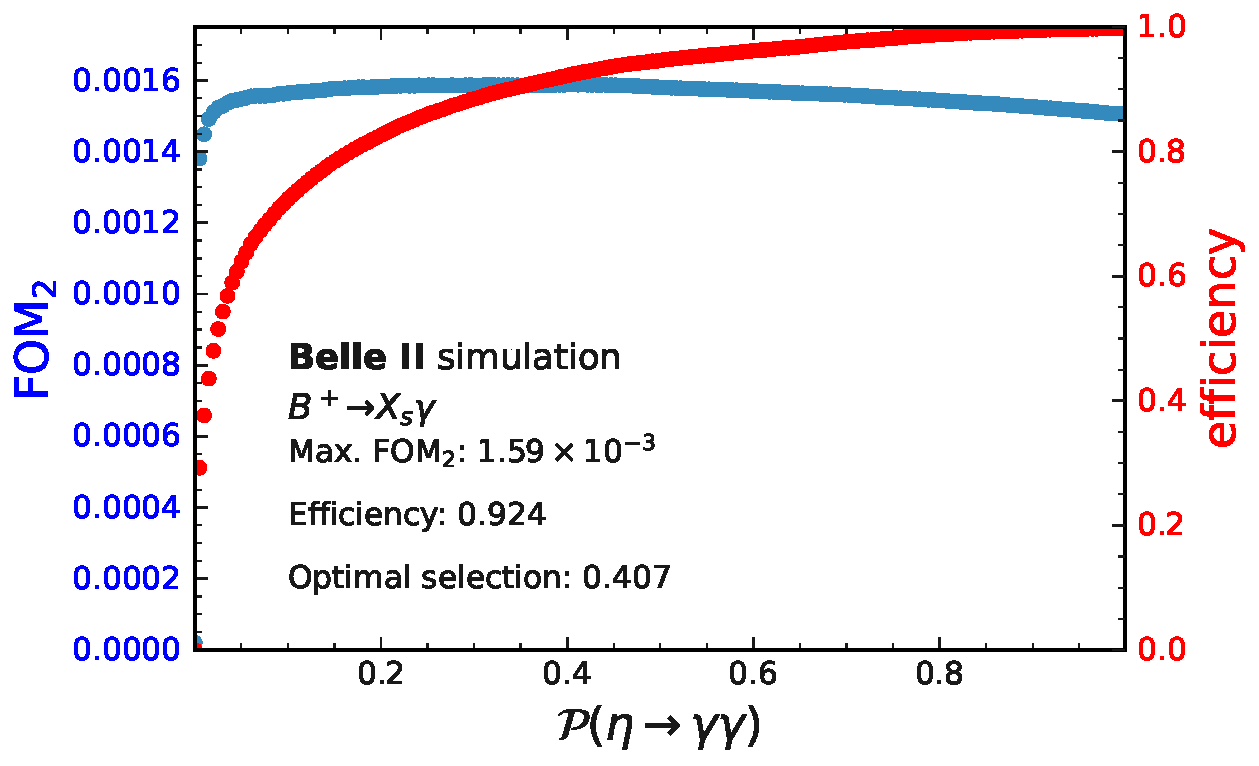
\includegraphics[width=0.3\textwidth]{figures/continuum_suppression/Bp_etaVeto_optimisation_punzi.pdf}
        }
    \subcaptionbox{\label{fig:bz_zmva_optimisation}}{
            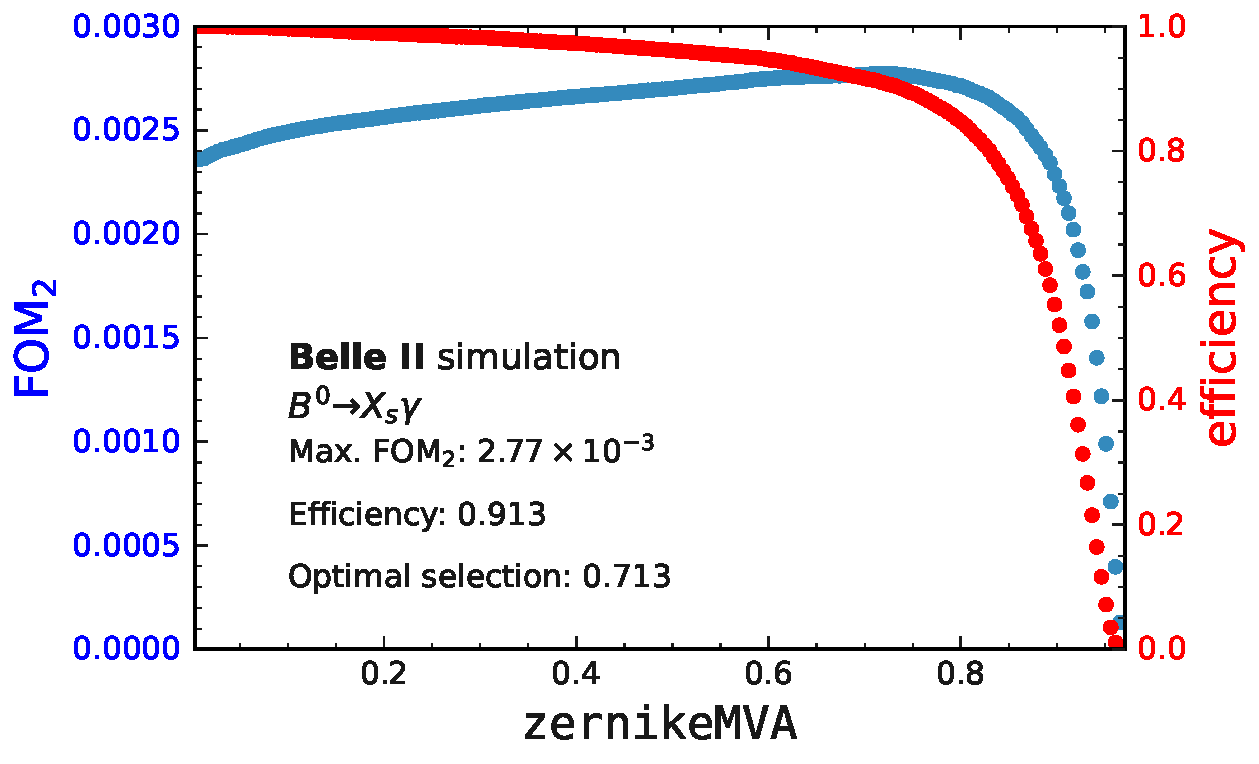
\includegraphics[width=0.3\textwidth]{figures/continuum_suppression/Bz_zernikeMVA_optimisation_punzi.pdf}
        }
    \subcaptionbox{\label{fig:bz_piveto_optimisation}}{
            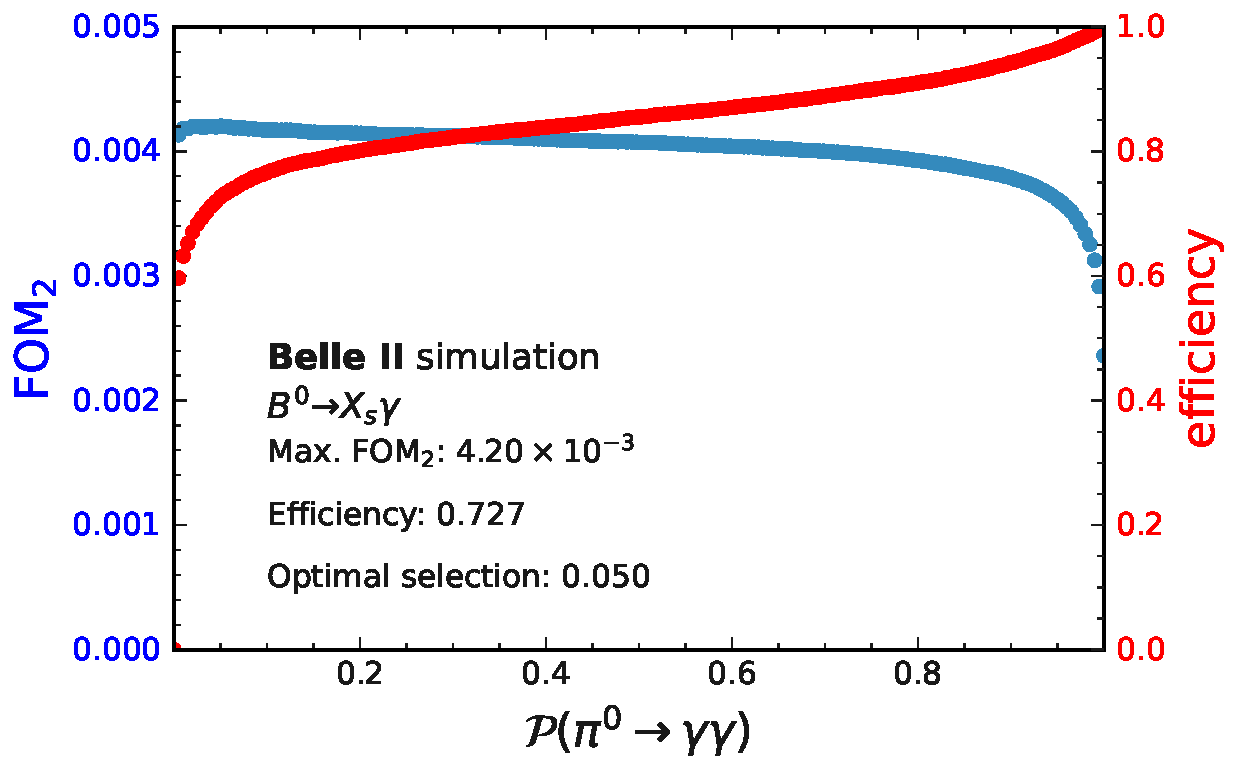
\includegraphics[width=0.3\textwidth]{figures/continuum_suppression/Bz_piVeto_optimisation_punzi.pdf}
        }
    \subcaptionbox{\label{fig:bz_etaveto_optimisation}}{
            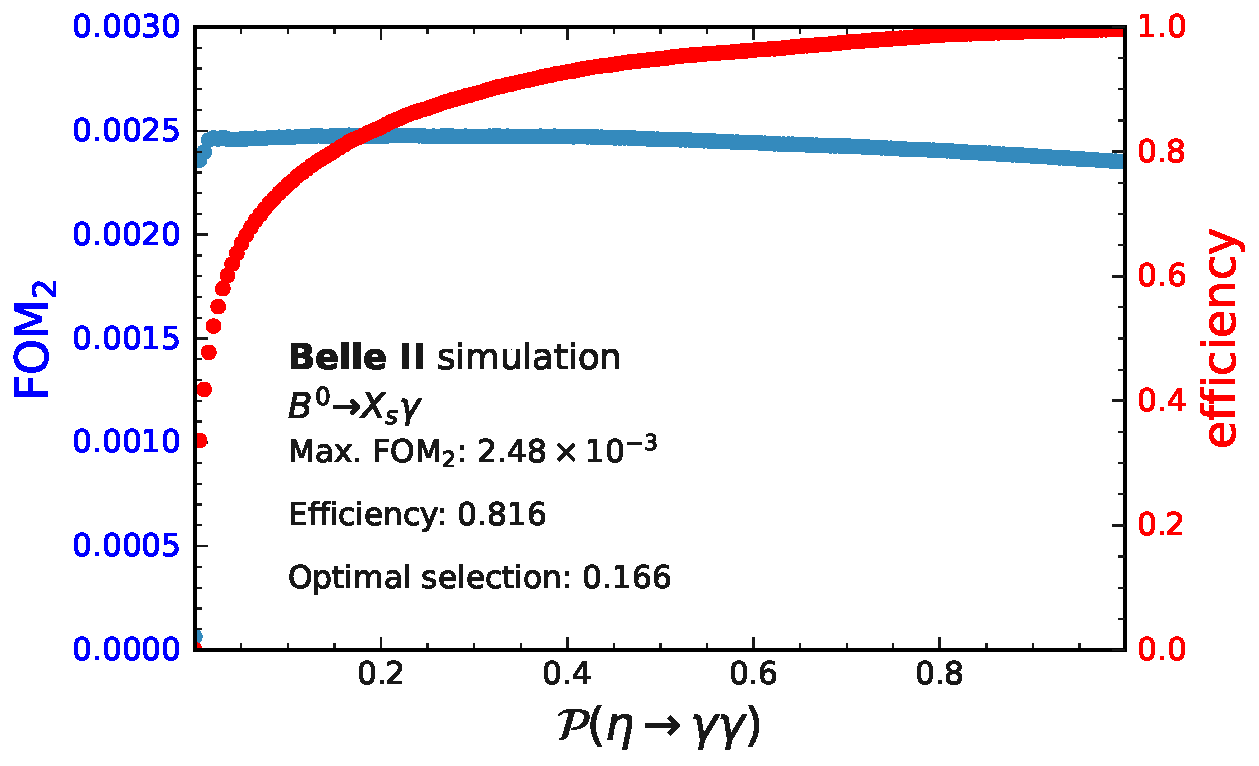
\includegraphics[width=0.3\textwidth]{figures/continuum_suppression/Bz_etaVeto_optimisation_punzi.pdf}
        }
    \caption{\label{fig:selection_optimisations} Optimal selection calculation for observables
    described in \Cref{sec:photon_selection} based on $\mathrm{FOM}_2$ (see \Cref{eq:punzi_fom}).
    For \BptoXsgamma events the tests are shown
    in \Cref{fig:bp_zmva_optimisation,fig:bp_piveto_optimisation,fig:bp_etaveto_optimisation},
    and for \BztoXsgamma in \Cref{fig:bz_zmva_optimisation,fig:bz_piveto_optimisation,fig:bz_etaveto_optimisation}.
    The figures show efficiency and $\mathrm{FOM}_2$ score calculated for 200 selections of \piVeto, \etaVeto and \ZMVA.
    The maximum value of $\mathrm{FOM}_2$, the corresponding selection and efficiency are shown as well.
    }
\end{figure}

The results between \Bp and \Bz modes, as well as using $\mathrm{FOM}_1$ and $\mathrm{FOM}_2$ are consistent, with only marginal differences.
Therefore, due to the model-independance of $\mathrm{FOM}_2$, this figure-of-merit will be the only one discussed henceforth.
At this stage, it is unnecessary to choose the `best' selection, 
as another simultaneous optimisation will be performed later, together with continuum suppression \BDT output in \Cref{sec:final_optimisation}.
The main goal is to reduce the sample size to include only relevant data, such that the trained \BDT can make decisions for difficult cases that are not easily distinguishable using simple selection.
Based on \Cref{fig:selection_optimisations}, pre-selections are chosen, which suppress background but retain most of the signal.
The requirement for a loose selection are tailored such that more roughly 75\% of \BtoXsgamma candidates are retained and are shown in \Cref{tab:preselections}.
They are chosen to be no tighter than their optimal selection and preferably considerably looser.

\begin{table}[htbp!]
    \centering
    \caption{\label{tab:preselections} Selections that remove background and misreconstructed candidates,
    preparing the reconstructed datasets \Cref{sec:reconstruction_overview} for continuum \BDT training (\Cref{sec:continuum_training}).
    A later optimisation will be used for a final candidate selection in \Cref{sec:final_optimisation}.
    }
    
    \begin{tabular}{|lr|}
    \hline
    Variable &    Loose selections \\
    \hline
    \ZMVA & $>0.5$ \\
    \piVeto            & $<0.4$ \\
    \etaVeto           & $<0.4$ \\
    
    \hline
    
    $B^+$ mode: $\gamma$ candidate retention efficiency & 75.4\% \\
    $B^0$ mode: $\gamma$ candidate retention efficiency & 76.7\% \\
    \hline
    \end{tabular}

\end{table}

The pre-selections improve the signal-to-background ratio by roughly an order of magnitude.
This can be clearly seen by comparing \Cref{fig:preselected_photons} with \Cref{fig:spectrum_after_reco}.
The scale at which \BtoXsgamma signal \MC scaled differs at about a factor of 10, meaning that the background reduced by approximately that amount due to these selections.


\begin{figure}[htbp!]
    \centering
    \subcaptionbox{\label{fig:bp_preselected_photons}}{
        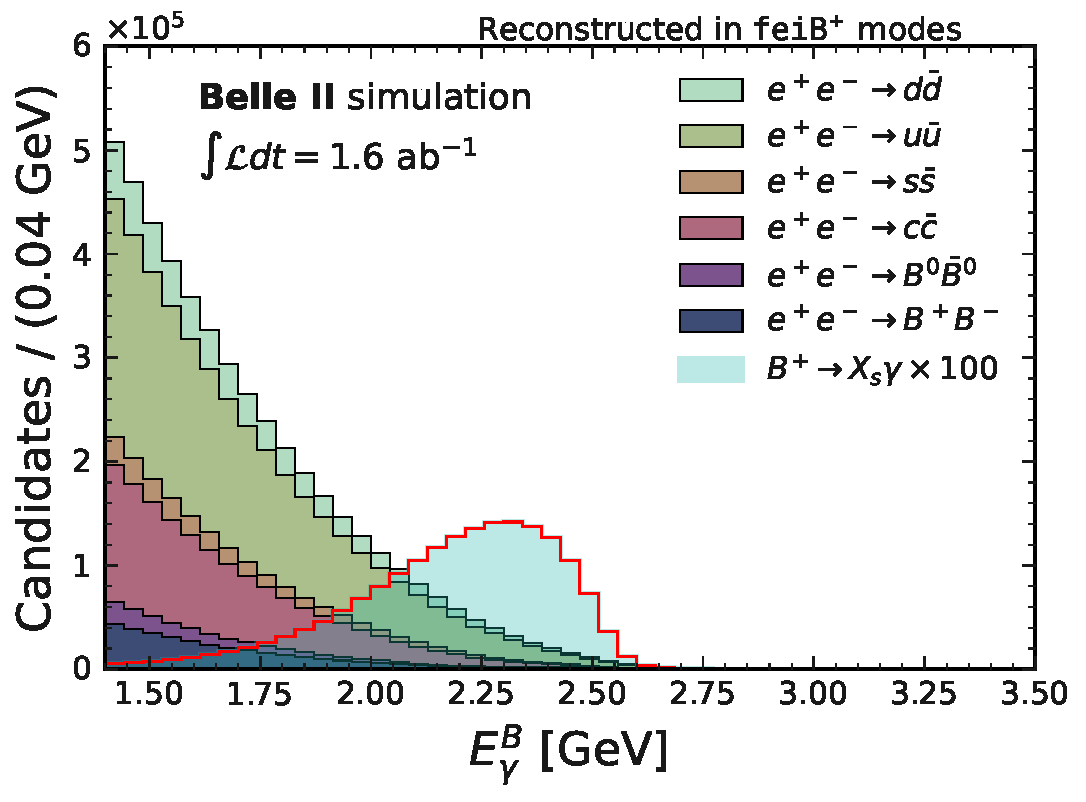
\includegraphics[width=0.395\textwidth]{figures/continuum_suppression/Bp_tagged_background_preselection.pdf}
    }
    \subcaptionbox{\label{fig:bz_preselected_photons}}{
        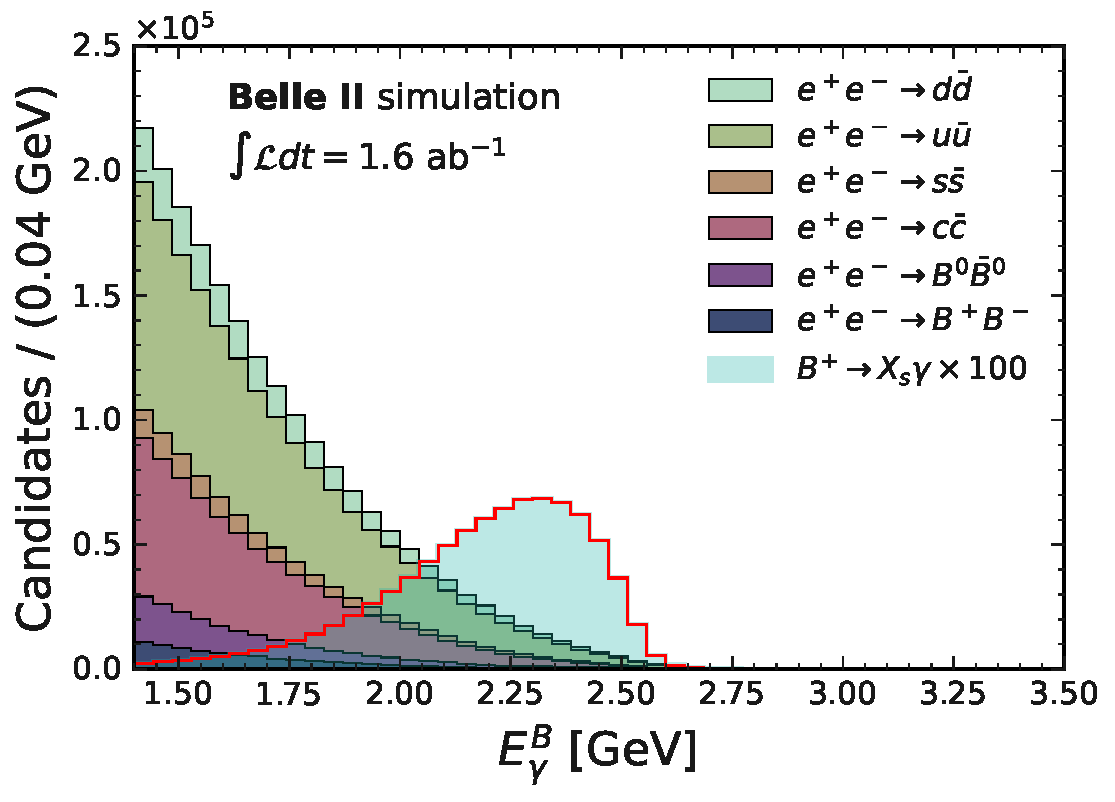
\includegraphics[width=0.395\textwidth]{figures/continuum_suppression/Bz_tagged_background_preselection.pdf}
        }
    \caption{\label{fig:preselected_photons} \BtoXsgamma spectrum in generic \MC after pre-selection for training the continuum suppression \BDT classifier.
    Overlaid are events from signal \MC where the photon comes from \BtoXsgamma, multiplied by a scaling factor.
    Compared to \Cref{fig:spectrum_after_reco}, the effectiveness of background suppression so far is apparent.
    These figures may include multiple tag entries per event.
    }
\end{figure}

Finally, many combinatorial tag-side candidates in \BB events may still appear contribute to the analysis at this stage.
A more detailed definition for a `well-reconstructed' tag will be explored later in \Cref{sec:good_tag_definition}.
At this stage, it is sufficient to acknowledge the fact that the vast majority of correctly reconstructed tag-side candidates is expected to have $\Mbc>5.27~\gevcc$.
Therefore, this requirement is also adopted for optimisation studies and training in \Cref{sec:continuum_features,sec:continuum_training,sec:continuum_validation}.

\subsection{Continuum suppression feature selection}\label{sec:continuum_features}

$B$ factory experiments and Belle II have a large selection of observables that can be utilised for continuum suppression and are suitable to be input as variables to a \BDT.
These observables combine describe the event-topology or particles in the event and are optimised to provide separation between \BB and \qqbar events.
There are two caveats that have to be kept in mind for the \BtoXsgamma analysis:
\begin{itemize}
    \item Generally, \BtoXsgamma event-topology may be different compared to \BB events. 
    \BtoXsgamma decays have a single jet-like $X_s$ system (while the other $B$ meson decays hadronically).
    This leads to a somewhat middle-case between a generic-\BB event and an \epem\ra\qqbar event, as it was illustrated in \Cref{fig:continuum_schematic}.
    \item Many of these observables contain momenta, angles or other parameters of some (or even all) particles in the event -- including the $X_s$ system and the photon.
    This may lead to a bias to the spectrum of $X_s$ system.
    Furthermore, even relatively small biases over many training features may be learnt by the \BDT and introduced to the spectrum.
    \item Some features may perform differently in real-data compared to simulation, due to unexpected differences in alignment, calibration or background distributions.
    As we use simulated data sets to train a \BDT in this analysis, such a comparison is crucial.
\end{itemize}
Given the mentioned points, it is important to test that observables used for the training provide adequate separation between \BtoXsgamma and \qqbar, while no bias is introduced to the photon energy spectrum.
Furthermore, this has to be well-represented in data.

In this analysis, the following observable categories are considered for separation between \epem\ra\qqbar and \BtoXsgamma:
\begin{itemize}
    \item Various thrust-based observables (\Cref{sec:thrusts});
    \item Sphericity and aplanarity (\Cref{sec:sphericity_aplanarity});
    \item Harmonic moments (\Cref{sec:harmonic_moments});
    \item Fox-Wolfram moments (\Cref{sec:fox_wolfram_moments});
    \item Modified Fox-Wolfram moments (\Cref{sec:modified_fox_wolfram_moments});
    \item CLEO cones (\Cref{sec:cleo_cones});
    % \item Angular tag-$B$ meson observables (\Cref{sec:angular_features});
    \item Tag-$B$ meson vertex observables (\Cref{sec:vertex_features});
    \item Flavour tagger output for the tag-$B$ meson(\Cref{sec:flavour_tagger_outputs});
\end{itemize}

In total, this provides 75 potential training features that are tested to be uncorrelated to the photon energy spectrum and adequately described in simulation.
The tests use a metric of \textit{total divergence to the average} (often called \textit{Jensen-Shannon distance}) \cite{Lin:1991abc},
which is used to quantitatively evaluate the similarity between two distributions.
The Jensen-Shannon distance is bounded by 1 for two given probability distributions, $\mathbb{X}_1$ and $\mathbb{X}_2$:
\begin{equation}\label{eq:js_distance}
    0\leq\mathrm{JSD}(\mathbb{X}_1||\mathbb{X}_2) \leq1,
\end{equation}
where exactly similar distributions have a score of 0, and the score tends towards 1 when the distributions are highly-different.

Two tests are performed:
\begin{itemize}
    \item \textbf{Test 1}: $\mathbf{\EB,~\Estar~and~tag\mbox{-}side~\Mbc~bias~test}$:
    to ensure that the classifier does not indirectly select particular $X_s$ or tag-side $B$ channels,
    each tested potential training feature is separated into 5 equally populated regions (\textit{slices}) of \BtoXsgamma events in signal \MC.
    For this test, \BptoXsgamma and \BztoXsgamma are merged.
    In each of these regions, the distribution of \EB, \Estar and \Mbc is compared.
    The Jensen-Shannon distance is required to not be larger than 6\% between any two given slices of a training feature.
    The requirement to pass \textbf{Test 1} has been chosen by observing the typical values of the agreement shown by the tested unbiased distributions.
    If this requirement is not passed by at least one of the distributions (\EB, \Estar or \Mbc), the feature is excluded from the list of final \BDT training features.
    \item \textbf{Test 2}: $\mathbf{\epem\ra\qqbar~data\mbox{-}simulation~similarity~test}$:
    to ensure that simulations adequately describe the data sets that we aim to suppress.
    This test is only performed if \textbf{Test~1} is passed.
    As this is a blinded analysis, off-resonance data samples are used, which only contain \epem\ra\qqbar events.
    In this case, the Jensen-Shannon distance is calculated between 
    the area-normalised distribution of a training feature in off-resonance data set,
    and the area-normalised distribution of a training feature in \epem\ra\qqbar simulation.
    The metric is required to be no more than 10\%.
    The looser requirement is adopted here, due to the fact that some difference is expected between the distributions,
    as the collision energy in off-resonance data set is different to the one in on-resonance simulation that is used in this analysis.
    Furthermore, an overall smaller off-resonance data set ($\sim19~\invfb$, see \Cref{sec:data_samples}) may have certain difference due to poissonian fluctuations.
\end{itemize}

The tested distributions have the selections from \Cref{sec:preselection} included, except for the case of off-resonance dataset, where the $\Mbc>5.27~\gevcc$ requirement is lifted.
For every event, when more than one tag-side candidate $B$ candidate exists, a random one is picked.
The application of \textbf{Test~1} with exact definitions for the 81 observables are shown in \Cref{sec:appendix_continuum_features}.

Out of 75 potential training features, 27 pass through the requirements of \textbf{Test~1}.
These are passed to \textbf{Test~2}
\textbf{Test~2}, owing to excellent calibration and simulation quality of Belle II, removes a single feature.
The results for the 26 final observables that pass both test requirements and will be used as features in the \BDT training
are shown in \Cref{tab:passing_test1}.

\begin{table}[htbp!]
    \centering
    \caption{\label{tab:passing_test1}The training features for the \epem\ra\qqbar suppression
    that pass the requirements of \textbf{Test~1} (see \Cref{sec:appendix_continuum_features}) and \textbf{Test~2} (see \Cref{sec:appendix_continuum_features_datamc}).
    The table also shows the value of the Jensen-Shannon distances for each observable for the different requirements of both tests.
    Exact definitions of these quantities is provided in \Cref{sec:appendix_continuum_features}.
    Observable groups follow those introduced in the text.
    }   
    \begin{tabular}{l|c|c|c|c|}
    \multirow{3}{*}{Feature name} & \multicolumn{4}{|c|}{Jensen Shannon Distances [$\sqrt{\mathrm{bit}}$]}\\
                                  & \multicolumn{3}{|c|}{Test~1} & Test~2\\
                                  & \EB& \Estar& \Mbc & Data-Sim.\\
    \hline
    \multicolumn{5}{c|}{\textbf{Thrust related}}\\
    \hline
    $\cos\theta_{\mathrm{TB}\wedge\mathrm{TO}}$ & 0.03 & 0.01 & 0.04 & 0.02\\
    $\cos\theta_{\mathrm{TB}\wedge\mathrm{z}}$ & 0.01 & 0.01 & 0.02 & 0.01\\
    $T_{\mathrm{B}}$ & 0.04 & 0.03 & 0.04 & 0.06\\
    $\cos\theta_{\mathrm{T}}$ & 0.02 & 0.02 & 0.01 & 0.02\\
    \hline
    \multicolumn{5}{c|}{\textbf{Harmonic moments}}\\
    \hline
    $B_{1}^T$ & 0.05 & 0.05 & 0.02 & 0.01\\
    $B_{3}^T$ & 0.04 & 0.03 & 0.01 & 0.03\\
    \hline
    \multicolumn{5}{c|}{\textbf{CLEO cones}}\\
    \hline
    $\mathtt{CC}^B_0$ & 0.04 & 0.03 & 0.03 & 0.03\\
    $\mathtt{CC}^B_1$ & 0.03 & 0.03 & 0.02 & 0.03\\
    $\mathtt{CC}^B_2$ & 0.04 & 0.03 & 0.02 & 0.01\\
    $\mathtt{CC}^B_3$ & 0.05 & 0.05 & 0.02 & 0.02\\
    $\mathtt{CC}_0$ & 0.05 & 0.05 & 0.02 & 0.02\\
    $\mathtt{CC}_3$ & 0.06 & 0.06 & 0.02 & 0.02\\
    \hline
    \multicolumn{5}{c|}{\textbf{Modified Fox-Wolfram moments}}\\
    \hline
    $H_{c4}^{so}$ & 0.05 & 0.04 & 0.02 & 0.02\\
    $H_{m2}^{so}$ & 0.03 & 0.03 & 0.02 & 0.02\\
    $H_{m4}^{so}$ & 0.03 & 0.03 & 0.01 & 0.01\\
    $H_{0}^{oo}$ & 0.03 & 0.02 & 0.02 & 0.04\\
    \hline
    \multicolumn{5}{c|}{\textbf{Tag-$\mathbf{B}$ meson vertex observables}}\\
    \hline
    $z$ of tag-B & 0.01 & 0.01 & 0.01 & 0.02 \\
    $\Delta x$ of tag-B & 0.02 & 0.02 & 0.03 & 0.03\\
    $\Delta y$ of tag-B & 0.01 & 0.01 & 0.03 & 0.04\\
    $\Delta z$ of tag-B & 0.02 & 0.02 & 0.04 & 0.02\\
    $\Delta \tau$ & 0.04 & 0.03 & 0.02 & 0.02\\
    $\Delta z$ & 0.04 & 0.03 & 0.02 & 0.02\\
    $\Delta z_B$ & 0.04 & 0.03 & 0.02 & 0.02\\
    $\chi^2_{B_{\mathrm{ROE}};\mathrm{IP}}$ & 0.05 & 0.05 & 0.01 & 0.00\\
    $x_{B_{\mathrm{ROE}}}$ & 0.03 & 0.03 & 0.01 & 0.02\\
    $z_{B_{\mathrm{ROE}}}$ & 0.03 & 0.03 & 0.01 & 0.05\\
\end{tabular}

\end{table}

\subsection{Continuum suppression training}\label{sec:continuum_training}

As it was argued in \Cref{sec:continuum_features}, events containing \BtoXsgamma decays may have slightly different kinematic properties compared to a generic-\BB.
Although these differences, as seen in \Cref{sec:appendix_continuum_features_datamc} are not large, training a classifier to separate generic $\FourS\ra\BB$ and \epem\ra\qqbar events may lead to a suboptimal separation of \BtoXsgamma.

A more effective setup is to remove \BB events from generic \MC and supplement the leftover events with \BtoXsgamma events from signal \MC. 
In such a scenario, the classifier learns to distinguish between the signal decays and continuum events, without the additional ambiguity of including generic \BB decays.
All selections from \Cref{tab:preselections} are employed for the training datasets.

The training samples are prepared by creating a mixture of $100000$ \epem\ra\qqbar events and 100000 \BtoXsgamma events from the signal MC sample.
In each event, one $\gamma$ and $\B_{\mathrm{tag}}$ candidate combination is randomly chosen.
This requirement ensures that the same event cannot contribute multiple training entries.
The target variable for the training is defined as a $\mathtt{flag}$, which follows
\begin{equation}
    \mathtt{flag}=\begin{cases}
      0,\quad \mathrm{for}~\epem\ra\qqbar~\mathrm{events},\\ 
      1,\quad \mathrm{for}~\BtoXsgamma~\mathrm{events}.
      \end{cases}
\end{equation}
Half of the \epem\ra\qqbar training sample is taken \feiBp mode, and the other half is from \feiBz modes. 
For signal, half is taken from $\BptoXsgamma$ signal mode, the other half from $B^0$, irrespective of the \FEI mode.
An equivalent sample is prepared as the testing sample for the training.

The training is performed using a \texttt{FastBDT} algorithm, introduced in \Cref{sec:BDTs_theory}.
Four hyperparameters within \texttt{FastBDT} framework have to be chosen.
Hyperparameter optimisation is performed in a grid-like search, based on two quantities:
\begin{align}\label{eq:optimisation_criteria}
    \begin{split}
    \mathtt{AUC}_{\mathrm{test}}&;\\
    \Delta \mathtt{AUC} \equiv |\mathtt{AUC}_{\mathrm{train}}& - \mathtt{AUC}_{\mathrm{test}}|,\\
    \end{split}
\end{align}
where $\mathtt{AUC}_{\mathrm{train}/\mathrm{test}}$ is the \AUC score for training or testing samples.
A set of hyperparameters is sought, such that $ \mathtt{AUC}_{\mathrm{test}}$ is maximised, while $\Delta \mathtt{AUC}$ is minimised.
The results of hyperparameter optimisation are summarised in \Cref{tab:grid_search} and shown in \Cref{fig:hyper_param}
Larger depths, number of trees values are not explored, to avoid non-linear correlations which may be learnt by the classifier and would require additional studies to pinpoint.
Large shrinkage values are undesired, to ensure a slower learning rate of the classifier.

\begin{table}[htbp!]
    \centering
    \caption{\label{tab:grid_search}Hyperparameter optimisation based on a grid-search method.
    The four hyperparameters for the \texttt{FastBDT} algorithm are defined in \Cref{sec:BDTs_theory}.
    The optimal values are chosen based on criteria defined in \Cref{eq:optimisation_criteria}.
    They are shown in the right most column are taken as the parameters for the training.
    The corresponding $\mathtt{AUC}_{\mathrm{test}}$ and $\Delta \mathtt{AUC}$ are shown in \Cref{fig:hyper_param} and \Cref{fig:roc_curve}.
    }
    \begin{tabular}{l|c|c|}
    Hyperparameter     & Tested grid values       & Chosen optimal parameter \\
    \hline 
    depth              & \{1,2,3\}                  & 2    \\
    number of trees    & \{100,200,400,600,1000\} & 400  \\
    shrinkage          & \{0.01,0.05,0.1,0.3,0.5\}          & 0.1  \\
    training subsample & \{0.2,0.4,0.5,0.6,0.8\}  & 0.8  \\
\end{tabular}

\end{table}

\begin{figure}[htbp!]
    \centering
    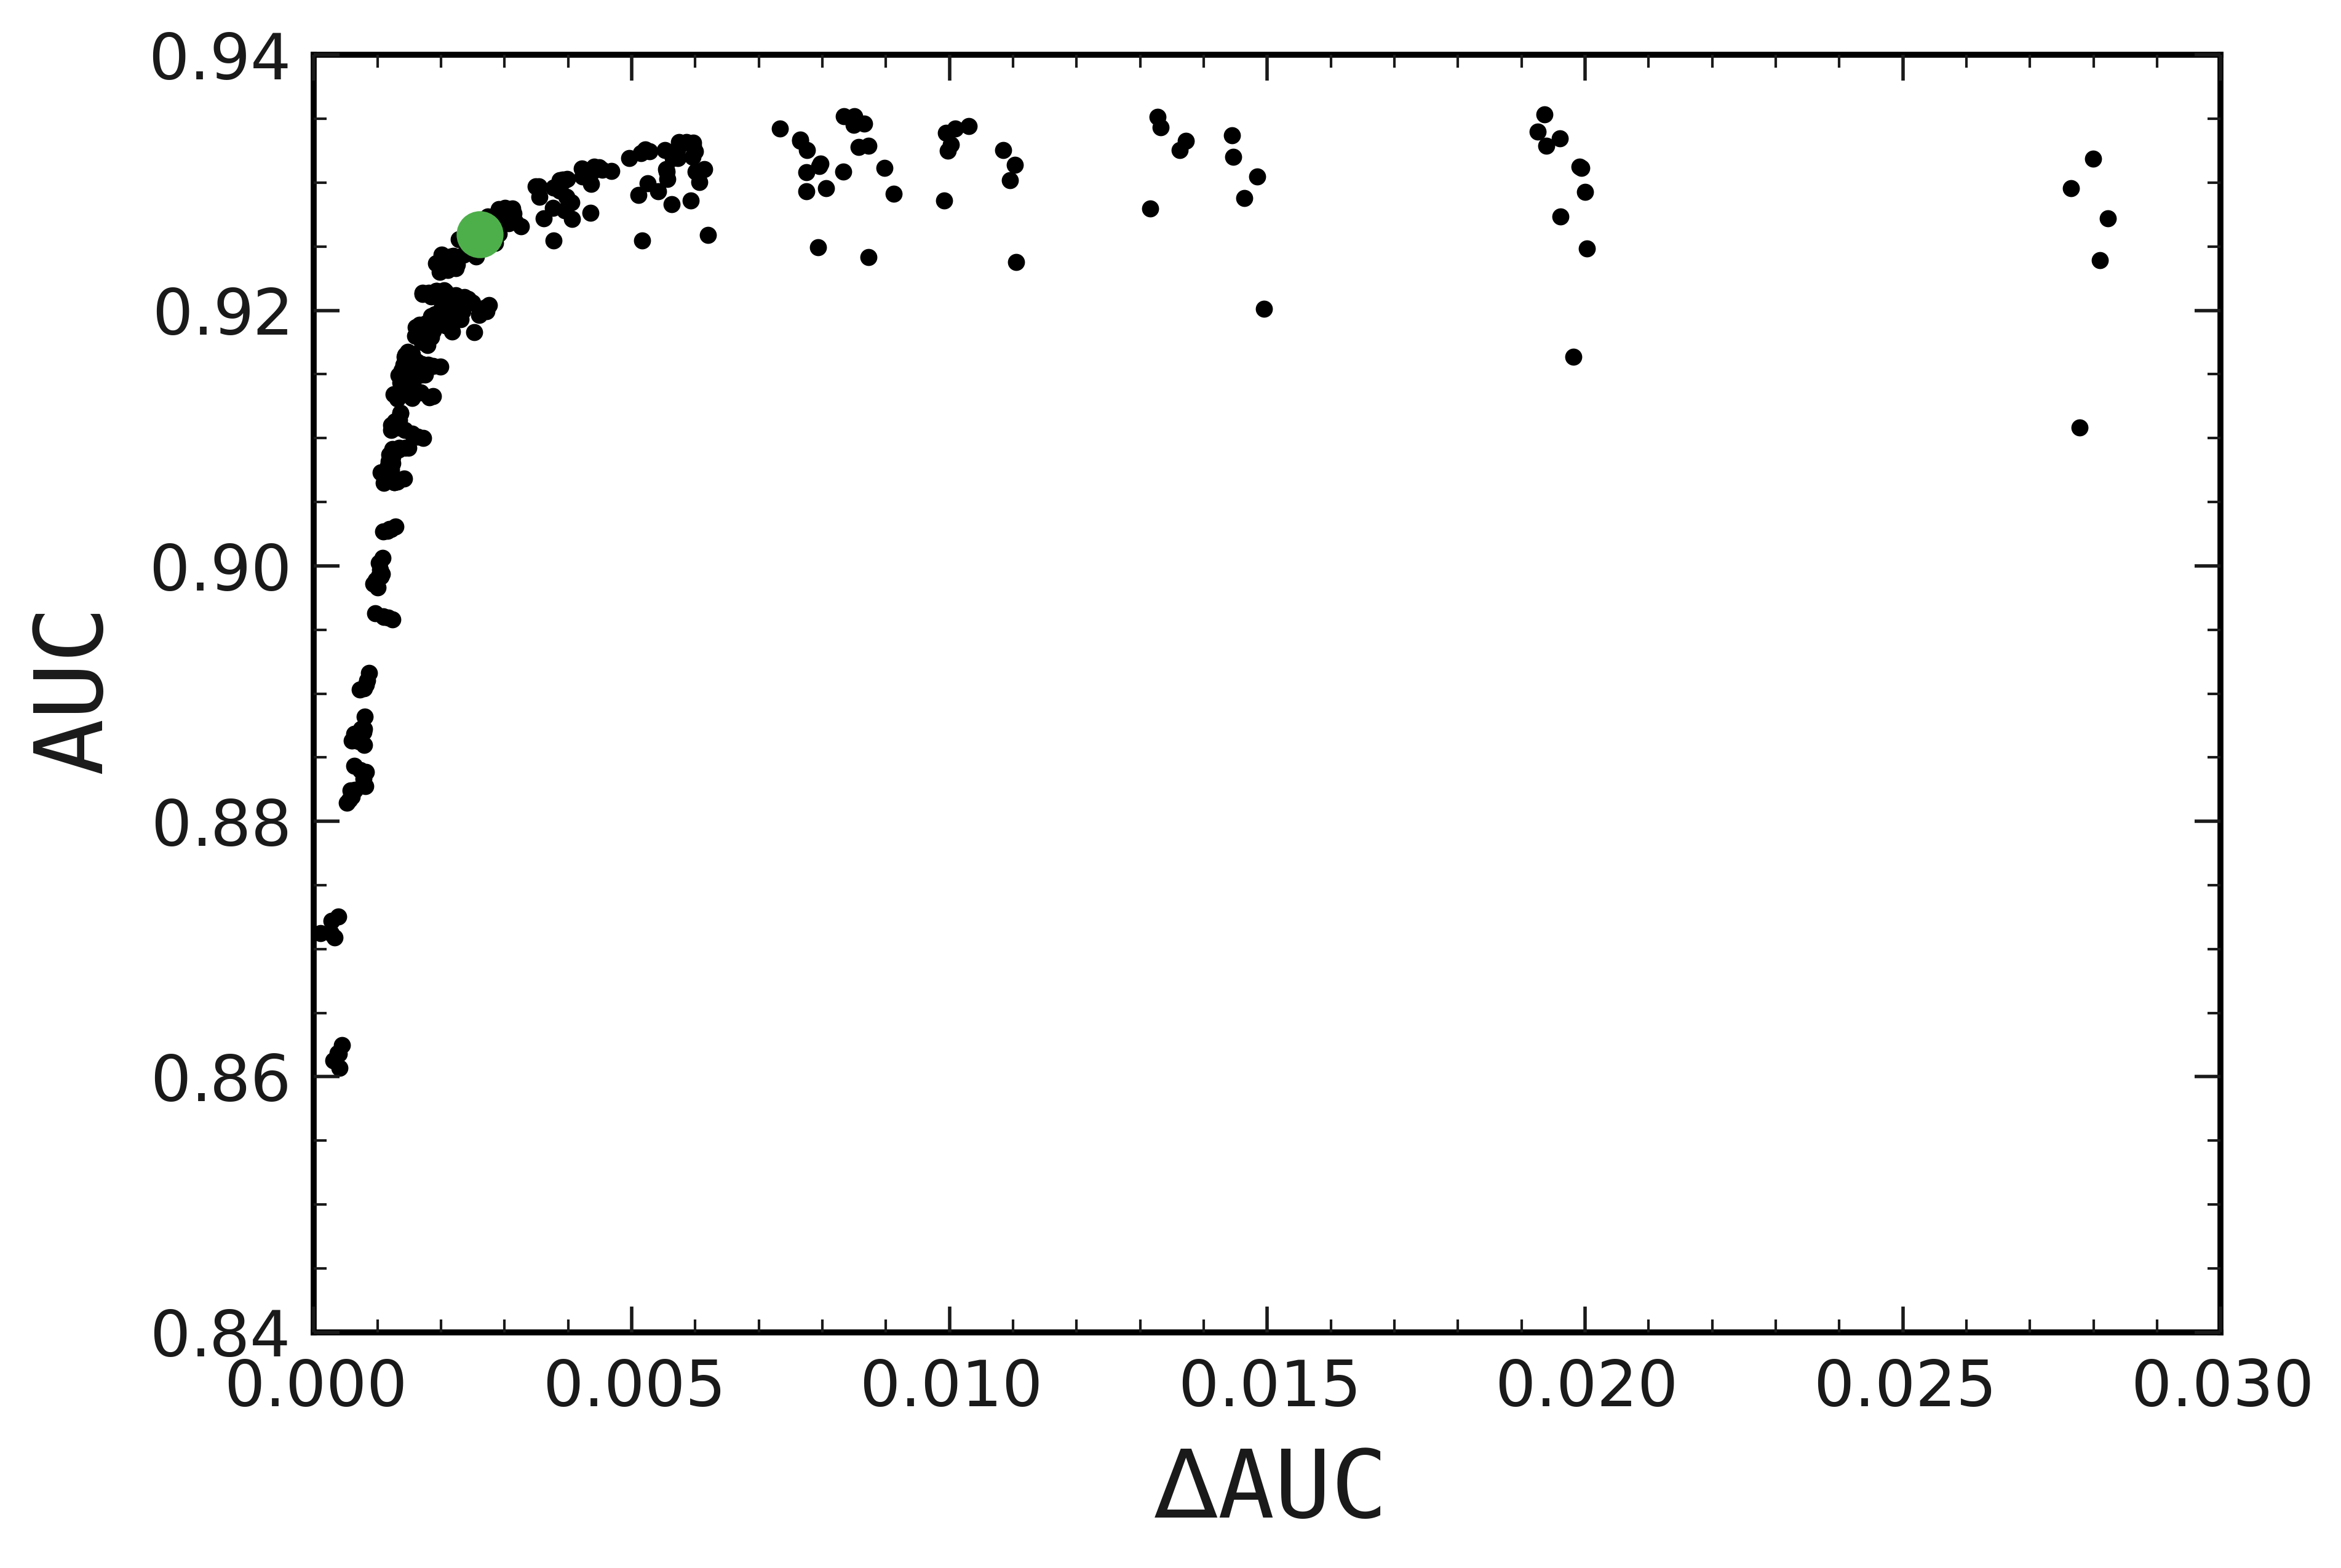
\includegraphics[width=0.45\textwidth]{figures/continuum_suppression/hyperpar_optimisation.png}
    \caption{\label{fig:hyper_param}Hyperparameter optimisation as a function of quantities defined in \Cref{eq:optimisation_criteria}.
    In total 375 working points are tested.
    The choice of parameters, shown in \Cref{tab:grid_search}, is represented by the enlargened green point.
    It is chosen in the threshold area, where $\mathtt{AUC}_{\mathrm{test}}$ gain saturates and $\Delta \mathtt{AUC}$ gain accelerates.
    }
\end{figure}

The training, with features from \Cref{tab:passing_test1} and hyperparameters from \Cref{tab:grid_search} is performed.
The normalised classifier output for test and train samples is shown in.
It is clearly seen that the classifier shows almost no bias, as the train and test samples agree very well.
This is further alluded by inspecting the ROC curve in.
The \AUC score is higher for the training sample (as expected in the case of a good training) but only by a minor amount.
Furthermore, the ROC curves themselves are practically indistinguishable.

\begin{figure}[htbp!]
    \centering
    \subcaptionbox{\label{fig:separation_curve}}{
    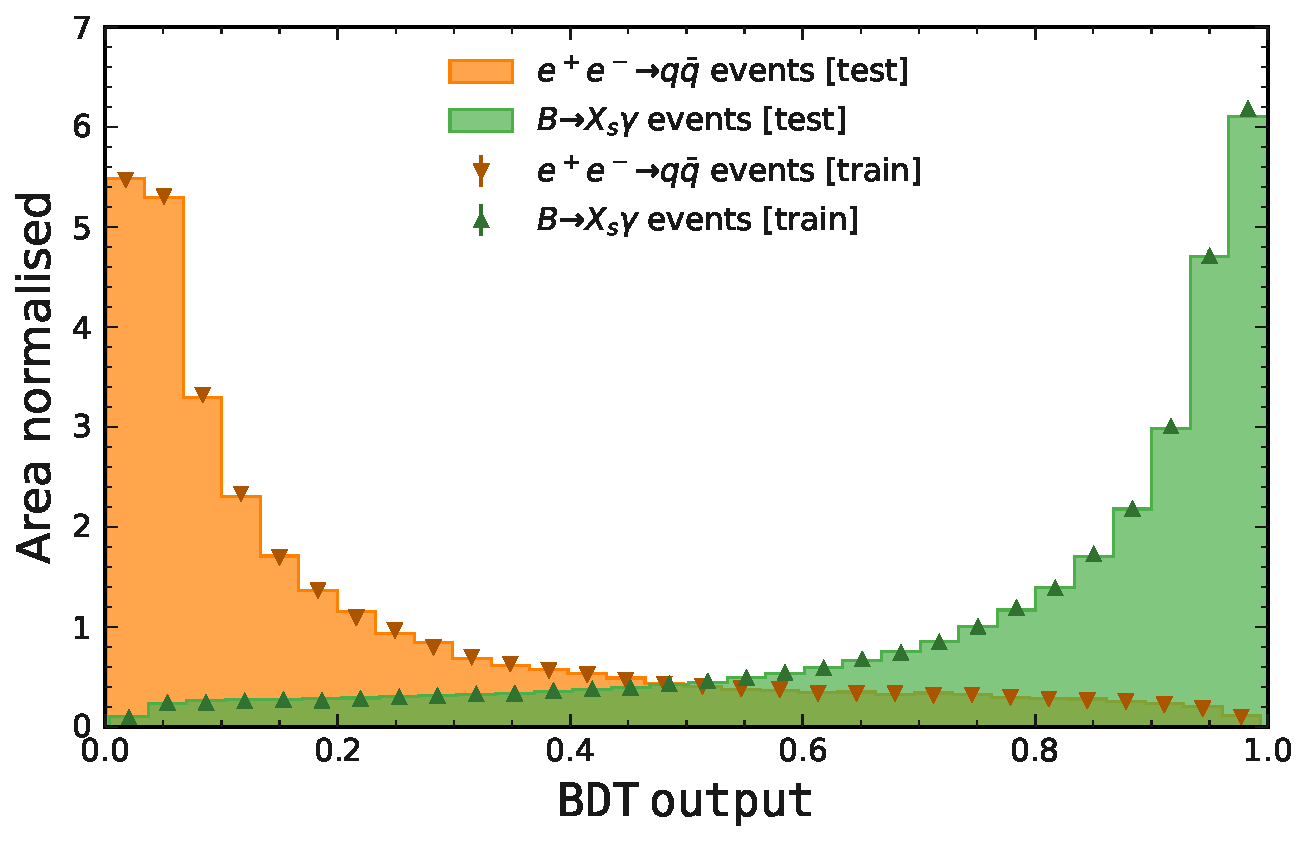
\includegraphics[width=0.45\textwidth]{figures/continuum_suppression/separation_curves.pdf}
    }
    \subcaptionbox{\label{fig:roc_curve}}{
        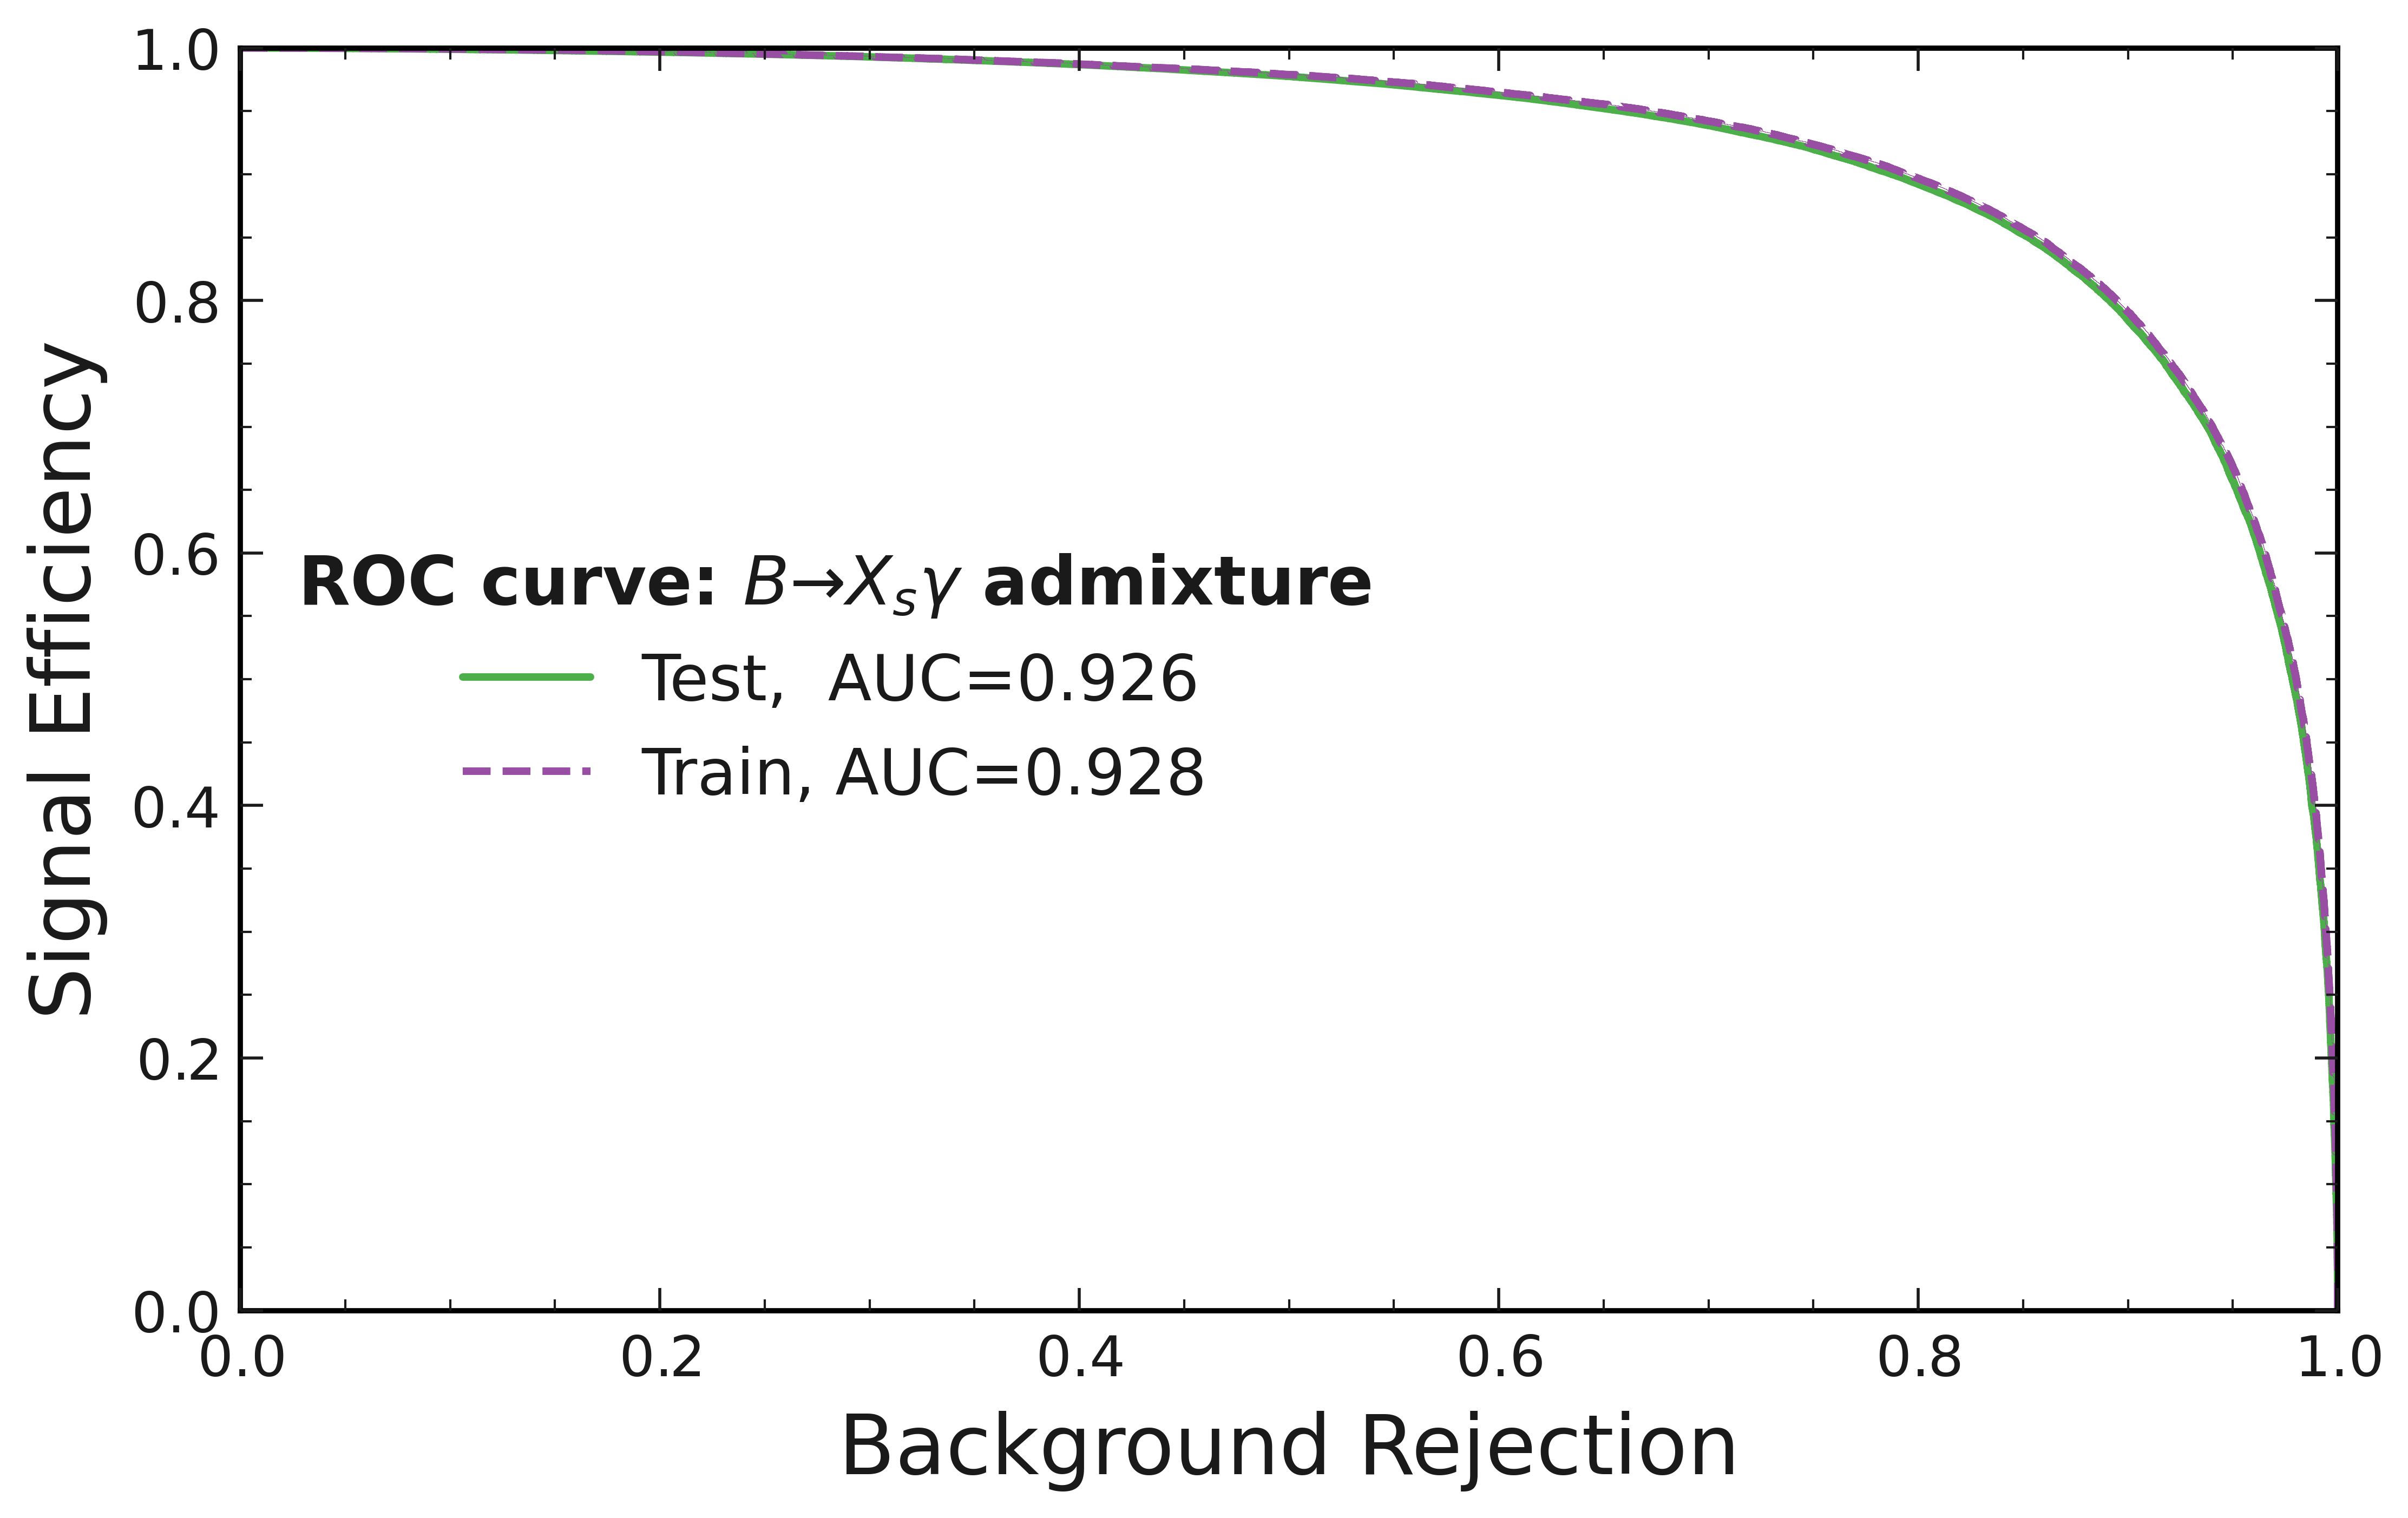
\includegraphics[width=0.45\textwidth]{figures/continuum_suppression/roc_curve.png}
    }
    \caption{\label{fig:training_evaluation} The training evaluation for this analysis.
    \Cref{fig:separation_curve} shows excellent separation between \epem\ra\qqbar and \BtoXsgamma samples, and excellent agreement between corresponding test and train samples.
    \Cref{fig:roc_curve} shows the \ROC curve of the training. 
    The test and train sample \AUC scores are close to unity and similar, alluding to a high-separation power that is observed, and no evidence of overtraining.
    }
\end{figure}

Using the tools provided by the \texttt{FastBDT} algorithm, a \textit{relative feature importance} is computed.
Particularly for \texttt{FastBDT}, it is computed by evaluating the decrease of the \AUC score if the feature is not included in the training dataset (for more details see Ref.\cite{Keck:2017gsv}.)
Therefore, it can be considered a quantitative measure of the impact of a feature on the final classifier output.
The figure depicting relative training observable importances is shown in \Cref{fig:feature_importance}. 
It is clearly seen that $\cos\theta_{\mathrm{TB}\wedge\mathrm{TO}}$ -- angle between thrust axis of the tag-$B$ candidate and everything else in the event. 
-- has by far the largest impact on the classifier.
This is not surprising after inspecting the individual separation power for the current problem in \Cref{sec:appendix_continuum_features_datamc}.
Other important separation features come from  $\Delta z_B$ \&  $\Delta z_B$, related to the longitudinal distance between the decay vertices,
thrust of the tag-$B$ meson, $T_B$ and CLEO cone variables $\mathtt{CC}_i$. 
For consistency, the events used in the training are removed from further analysis, although their impact is negligible.

\begin{figure}[htbp!]
    \centering
    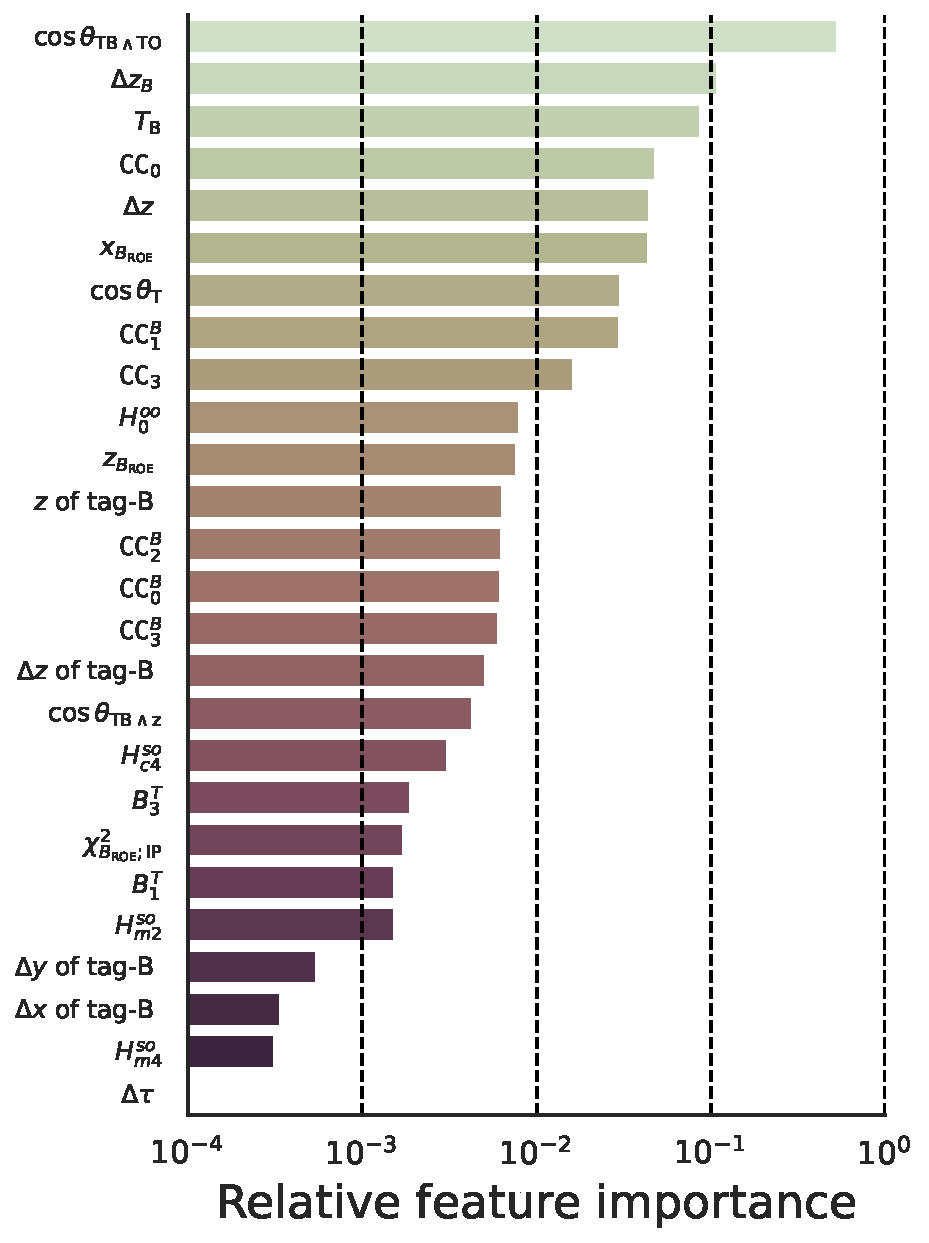
\includegraphics[width=0.45\textwidth]{figures/continuum_suppression/feature_importance.pdf}
    \caption{\label{fig:feature_importance} The relative feature importances of different observables used in the training.
    The definitions of these observables are provided in \Cref{sec:appendix_continuum_features}.
    The feature importance highlights a relative change in \AUC score when the observable is not included in the training.
    }
\end{figure}

\subsection{Continuum suppression validation}\label{sec:continuum_validation}

The resulting $\mathtt{BDT~output}$ is tested photon energy spectrum to further ensure the validity of the training.
Following the tests for bias of the average, median and $1\sigma$ percentiles in \Cref{sec:signal_photon_correlation},
the same study is performed for the training classifier output.
The result is shown in \Cref{fig:bdt_output_correlation} for the \BtoXsgamma admixture sample with the same requirements as the training sample.
No significant bias to any of the photon-energy spectrum quantities is observed in any of the bin.
In \Cref{fig:bdt_data_shape} the trained classifier output is also applied on off-resonance data to compare the shapes of off-resonance data and simulation.
Adequate agreement is observed, particularly in the high-$\mathtt{BDT~output}$ region where most signal lies.
The results seen in \Cref{fig:bdt_validation} validate the fact that the \BDT is prepared in an unbiased way and strongly suppresses the continuum events.

\begin{figure}[htbp!]
    \centering
    \subcaptionbox{\label{fig:bdt_output_correlation}}{
    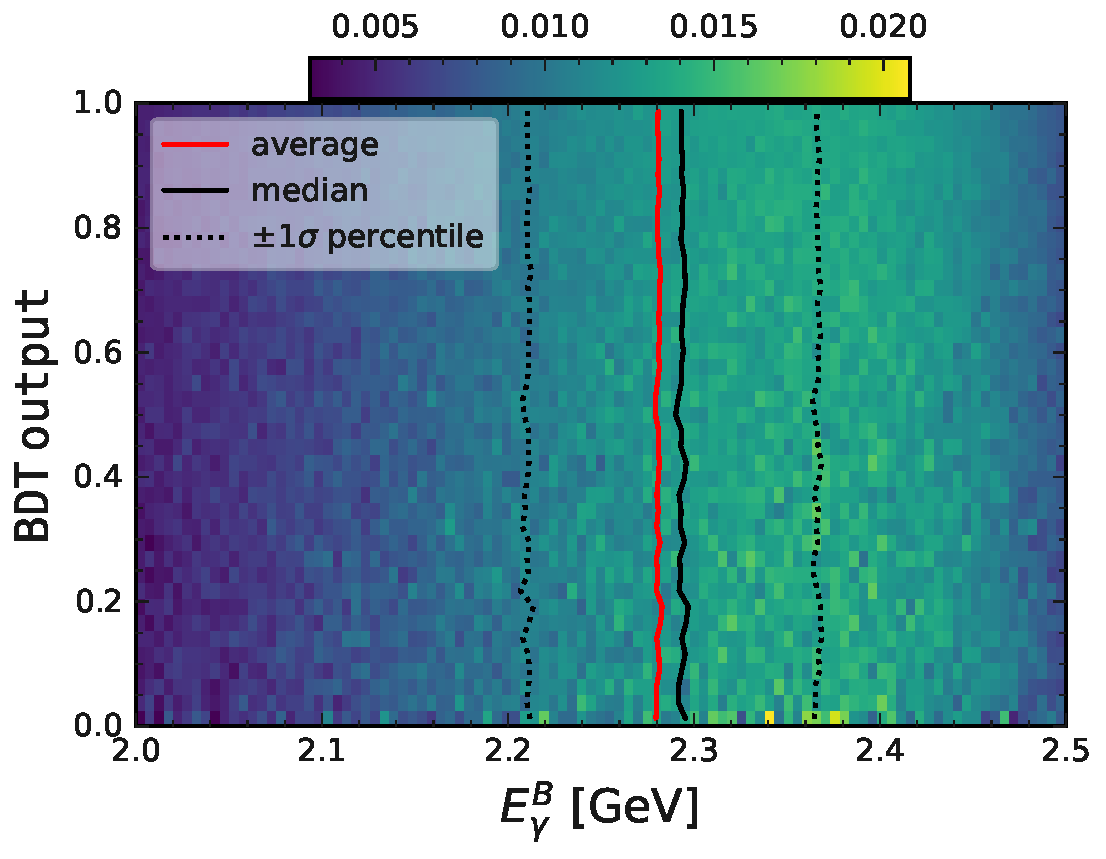
\includegraphics[width=0.4\textwidth]{figures/continuum_suppression/BDT_output_correlation.pdf}
    }
    \subcaptionbox{\label{fig:bdt_data_shape}}{
        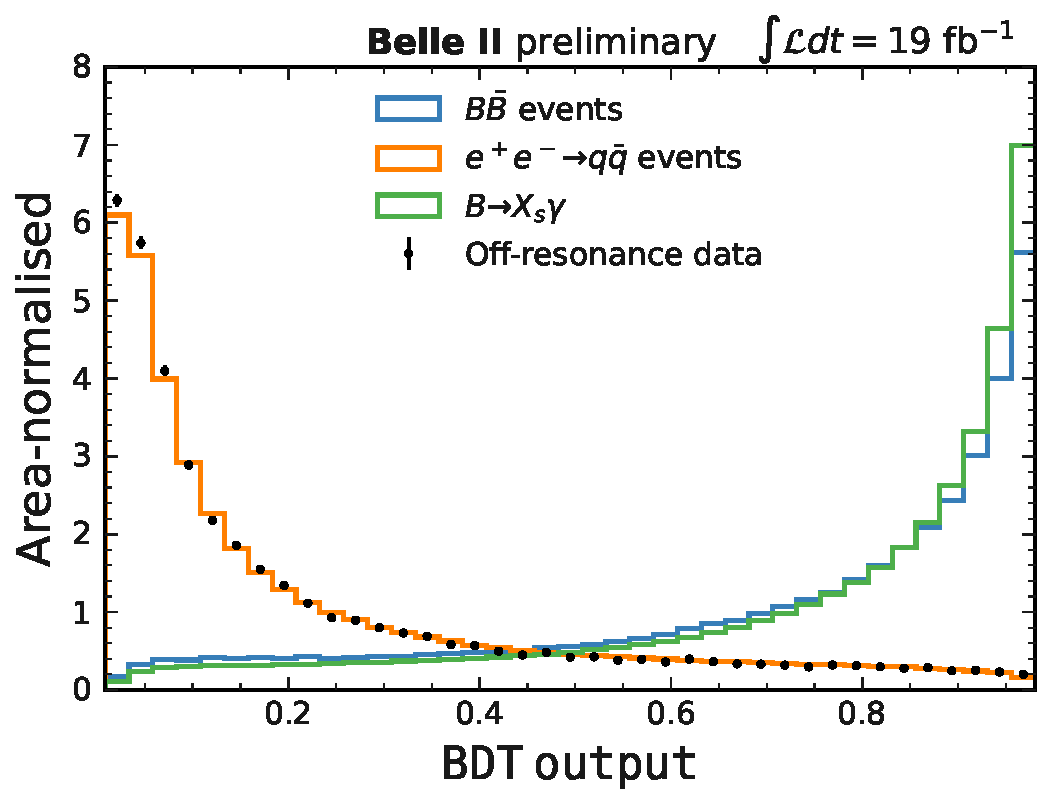
\includegraphics[width=0.4\textwidth]{figures/continuum_suppression/trained_bdtBDT_output_test.pdf}
        }
    \caption{\label{fig:bdt_validation} 
    Validation of the training described in \Cref{sec:continuum_training}.
    In \Cref{fig:bdt_output_correlation}, correlation tests for the trained classifier output described in \Cref{sec:continuum_training}, depicted as a 2D histogram.
    Each row is normalised, such that all bins within that row add up to 1.
    In red line, the average photon energy, $\expval{\EB}$, is shown as a function of the tested observable.
    In black and black-dotted lines -- median and $\pm 1 \sigma$ percentile values of \EB, respectively.
    No strong dependence can be observed in any of the quantities or the 2D maps.
    In \Cref{fig:bdt_data_shape}, the shape of \epem\ra\qqbar and off-resonance data is compared.
    It is seen that both simulated and off-resonance data sets are well separated from \BB and \BtoXsgamma simulation.
    }
\end{figure}

\section{Final selection optimisation}\label{sec:final_optimisation}
The last two sections introduced the selection to suppress photons originating in non-\mbox{\BtoXsgamma} decays, particularly from \piz and \eta decays (\Cref{sec:photon_selection}),
and the strategy suppress \mbox{\epem\ra\qqbar} events which were the dominant component in the selected data set (\Cref{sec:continuum_suppression}).
Although a preselection was already developped to prepare an adequate training sample for the \BDT, a more optimal (`tighter') selection is desired to ensure the optimal efficiency and purity of the selected sample.
This section will describe the approach taken to find this optimal selection, and calculate the efficiency loss for all applied selections.

\subsection{Simultaneous selection optimisation}\label{sec:simultaneous_optimisation}

After the pre-selection that prepared the data for training a \BDT in \Cref{tab:preselections}, a more robust strategy for tighter selections is developed.
In particular, \BDT output, \piVeto, \etaVeto and \ZMVA may be interconnected, in the sense that applying the selection on one of them, may influence a selection on the others. 
To find an optimal selection point, each selection is optimised in an iteration-based approach, 
where each requirement is optimised to a value that gives best figure-of-merit score individually,
while keeping the other requirements unvaried.
The individual optimisation are equivalent to that shown in \Cref{fig:selection_optimisations} and use figure-of-merit $\mathtt{FOM}_2$ defined in \Cref{eq:punzi_fom}.


In order to maximise the efficiency of events on kinematically well-reconstructed events, without adhering to a more strict definition at this stage, 
this procedure is performed on peaking events ($\Mbc >5.27~\gevcc$) and a single combination of the highest energy photon with a randomly selected tag-candidate per event.
The starting point for each selection correspond to values in \Cref{tab:preselections}.
The starting $\mathtt{BDT~output}$ selection is chosen at 0.5. 
The \BtoXsgamma admixture of charged and neutral modes is used.
The \epem\ra\qqbar and generic \BB background events from \feiBp and \feiBz modes are merged.
This aims to reproduce `realistic' data conditions, where different efficiencies may be related due to different \FEI and selection behaviour on charged and neutral modes.

After performing the optimisation for each selection, the optimisation round is repeated 9 more times.
The selections converge and do not vary after round 3 optimisation.
The converged value that is found is shown in \Cref{tab:interative_optimisation}.

\begin{table}[htbp!]
    \centering
    \caption{\label{tab:interative_optimisation} Optimal selections chosen for this analysis, based on the iterative approach described in \Cref{sec:simultaneous_optimisation}.
    The values for $\mathtt{BDT~output}$ and \ZMVA are chosen near those that are found optimal.
    For \piVeto and \etaVeto the choice is made based on the availability of data-simulation agreement studies performed at Belle II.
    At the time of preparing the analysis, 
    only studies with \piVeto and \etaVeto thresholds 
    up to 0.4 were analyses and appropriate correction factors supplied (see \Cref{sec:piz_eta_calibration}).
    }
    \begin{tabular}{|l|c|c|}
        \hline
        Variable &    Figure-of-merit maximised at & Final chosen \\
        \hline
        \ZMVA                      & $>0.629$ & 0.6\\
        \piVeto                    & $<0.258$ & 0.4\\
        \etaVeto                   & $<0.036$ & 0.4\\
        $\mathtt{BDT~output}$      & $>0.798$ & 0.8\\
        \hline
\end{tabular}
\end{table}

For \piVeto and \etaVeto, the found selection is relatively tight, if inspecting \Cref{fig:bp_piveto,fig:bz_piveto,fig:bp_etaveto,fig:bz_etaveto}.
Furthermore, at the time of preparation of the analysis desribed, studies regarding the \piVeto and \etaVeto applicability to such tight selections were not done.
Therefore, it was decided to not tighten this selection further than the pre-selection value obtained in \Cref{tab:preselections}.
Repeating the study while keeping \piVeto and \etaVeto selection at 0.4 yields compatible results to those shown in \Cref{tab:interative_optimisation}.
Therefore, other selections are chosen based on the optimal value from the initial 10 iterations.

\subsection{Summary and efficiency of all analysis selections}\label{sec:selection_summary}

A table, summarising all the selections and \BDT training results from \Cref{sec:photon_selection,sec:continuum_suppression,sec:final_optimisation},
and listing the final \BtoXsgamma candidate retention, is shown in \Cref{tab:cutflow}.
The retention, in this case, is defined as:
\begin{equation}\label{eq:loose_efficiency}
    r_{\mathrm{cand}} = \frac{N_{\BtoXsgamma}~\mathrm{candidates~after~cut}}{N_{\BtoXsgamma}~\mathrm{no~cut}},
\end{equation}
which is an estimate, as it may include multiple tag-side $B$ candidates.
For the calculation of this table, the $\Mbc>5.27~\gevcc$ requirement is no longer applied and all tag-$B$ meson candidates are maintained (i.e. high-energy photon candidates may contribute more than once per event).

\begin{table}[htbp!]
    \centering
    \caption{\label{tab:cutflow} The summary table of all selections and their retentions, based on \Cref{eq:loose_efficiency}.
    The selections listed here are applied on official Belle II \feiBp and \feiBz samples, described in \Cref{sec:reconstruction_overview}.
    The columns show efficiency costs for \BtoXsgamma events, calculated on signal \MC, continuum and \BB events, both of which are calculated on generic \MC.
    It can be seen that continuum events are suppressed by roughly two orders of magnitude, whereas generic-\BB decays -- by more than an order of magnitude.
    }
    \centering
\begin{minipage}[c]{0.49\textwidth}
    \centering
    \feiBp mode reconstruction
    \resizebox{1\textwidth}{!}{
        \begin{tabular}{lrrr}
            \multirow{2}{*}{Selection}   & \BtoXsgamma & Continuum &    \BB events \\
                                         & \multicolumn{3}{c}{Retention}     \\       
            \hline                                        
            none                  & 1.0000 & 1.0000    & 1.0000 \\
            $E_{\gamma}$ rank $= 1$     & 0.9979 & 0.9660    & 0.9762 \\
            $\ZMVA>0.6$        & 0.9435 & 0.6543    & 0.6957 \\
            $\piVeto<0.4$ & 0.8309 & 0.2145    & 0.3140 \\
            $\etaVeto<0.4$  & 0.9212 & 0.7637    & 0.7676 \\
            $\mathtt{BDT~output}>0.8$   & 0.5615 & 0.0253    & 0.4854 \\
            tag-$\Mbc>5.245~\gevcc$         & 0.9485 & 0.8863    & 0.9287 \\
            \hline
            all                   & 0.4211 & 0.0045    & 0.0731 \\
            \end{tabular}
            
    }
\end{minipage}
\begin{minipage}[c]{0.49\textwidth}
    \centering
    \feiBz mode reconstruction
    \resizebox{1\textwidth}{!}{
        \begin{tabular}{lrrr}
            \multirow{2}{*}{Selection}   & \BtoXsgamma & Continuum &    \BB events \\
                                         & \multicolumn{3}{c}{Retention} \\
            \hline 
            none                  &1.0000 & 1.0000 & 1.0000 \\
            $E_{\gamma}$ rank $= 1$     &0.9982 & 0.9680 & 0.9791 \\
            $\ZMVA>0.6$        &0.9449 & 0.6570 & 0.6899 \\
            $\piVeto<0.4$ &0.8411 & 0.2221 & 0.3235 \\
            $\etaVeto<0.4$  &0.9272 & 0.7824 & 0.7739 \\
            $\mathtt{BDT~output}>0.8$  &0.5538 & 0.0251 & 0.4791 \\
            tag-$\Mbc>5.245~\gevcc$          &0.9461 & 0.8837 & 0.9230 \\
            \hline
            all                   &0.4206 & 0.0047 & 0.0735 \\
            \end{tabular}
    }
\end{minipage}
\end{table}

\Cref{tab:cutflow} shows that the background suppression procedure roughly halves the number of available \BtoXsgamma events in the sample.
However, the background candidates from \epem\ra\qqbar processes are reduced 200 times, to less than 0.5\% of the original value.
Furthermore, generic-\BB event contribution is estimated at about 7\% of the original, which means more than an order of magnitude suppression is achieved.
The photon energy spectrum, after these selections have been applied is shown in \Cref{fig:spectrum_after_optimisation}.
Compared with previous iterations of this figure, e.g.\Cref{fig:spectrum_after_reco}, a much better signal-to-background ratio is clearly visible.

\begin{figure}[htbp!]
    \centering
    \subcaptionbox{\label{fig:spectrum_after_optimisation_bp}}{
        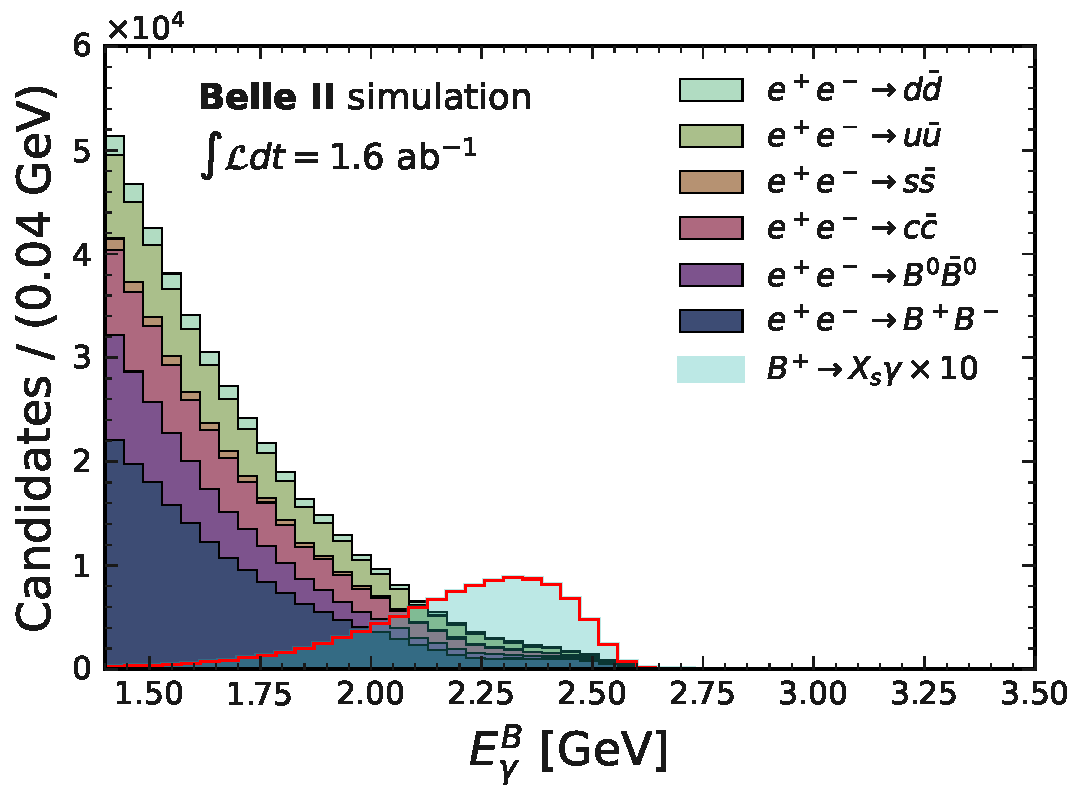
\includegraphics[width=0.4\textwidth]{figures/final_optimisation/Bp_tagged_background_optimal.pdf}
    }    
    \subcaptionbox{\label{fig:spectrum_after_optimisation_bz}}{
        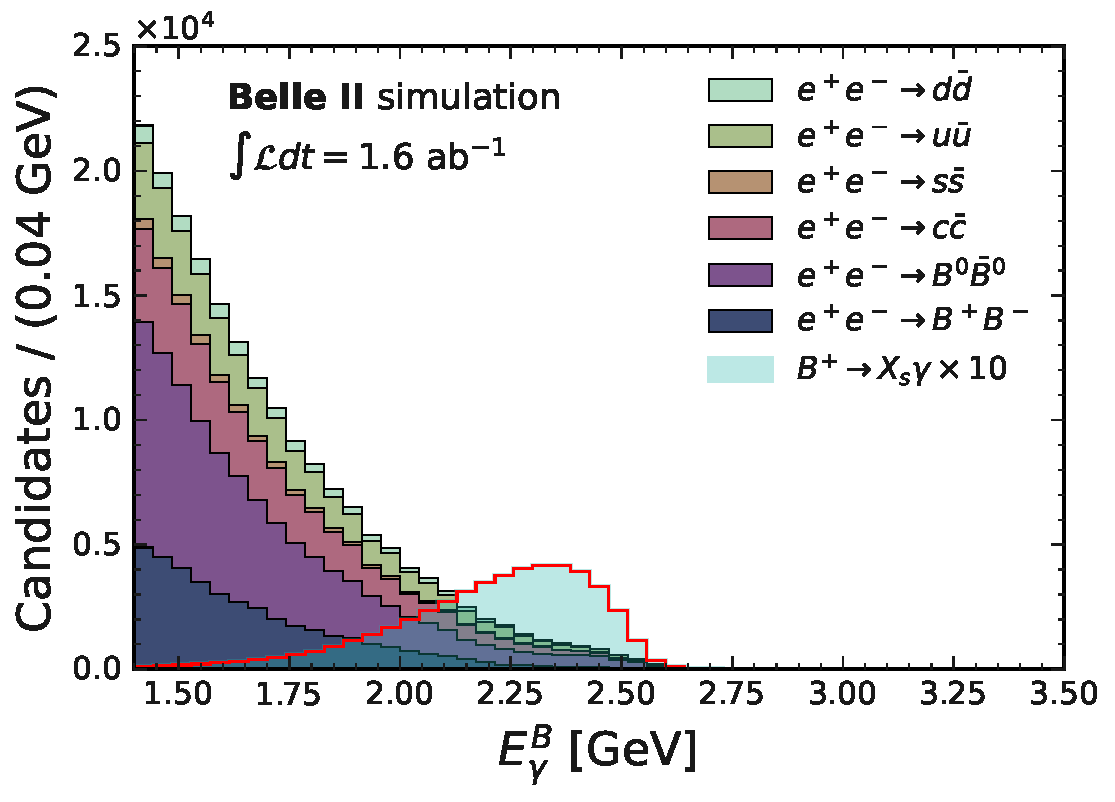
\includegraphics[width=0.4\textwidth]{figures/final_optimisation/Bz_tagged_background_optimal.pdf}
    }    
    \caption{\label{fig:spectrum_after_optimisation}\BtoXsgamma spectrum in generic \MC after event reconstruction and optimised selections applied, lised in \Cref{tab:cutflow}.
    Overlaid are events from signal \MC where the photon comes from \BtoXsgamma, multiplied by a scaling factor, with the same selections applied.
    These figures may include a high-energy photon combined with multiple tag entries per event and can be compared directly with \Cref{fig:spectrum_after_reco}.
    Compared to the post-reconstruction figure, the scaling factor for \BtoXsgamma is 100 times lower.}
\end{figure}


\section{Tag-side \texorpdfstring{\B}{B} candidate selection}\label{sec:tag_selection}
In \Cref{sec:reconstruction_overview} it was discussed that in about a half of all reconstructed events there exists more than one tag-side candidate.
That does not take into account the overlap between \feiBp and \feiBz mode -- which further enhances this effect.
Performing the best tag-side $B$ candidate selection is important, as multiple entries per event should not be included in the final sample.
However, the interest in this analysis lies in the signal side which decays as \BtoXsgamma, which means that a standard Belle II `truth-matching' procedure is too strict.
In principle, our requirement is to only reconstruct a sample of tag $B$ mesons that \textit{give provide good kinematic constraints to the signal side}.
In this section, these definition for best-candidate selection are discussed more broadly and
 a concrete definition for tag-$B$ mesons with correctly reconstructed kinematic properties is introduced.

\subsection{Selection within the same \texorpdfstring{\FEI}{FEI} mode}

The number of tag-side candidates for \feiBp and \feiBz modes, after the optimised selections in \Cref{tab:cutflow},
is shown in \Cref{fig:fei_tag_reco_candidates_post_optimisation}.
Overall, comparing to \Cref{fig:fei_tag_reco_candidates}, the candidate fractions are similar --
which attests to the fact that background (and particularly continuum) suppression was done without introducing a bias in preferentially selecting events with large \feiProb in \Cref{sec:continuum_suppression,sec:photon_selection}.

\begin{figure}[htbp!]
    \centering
    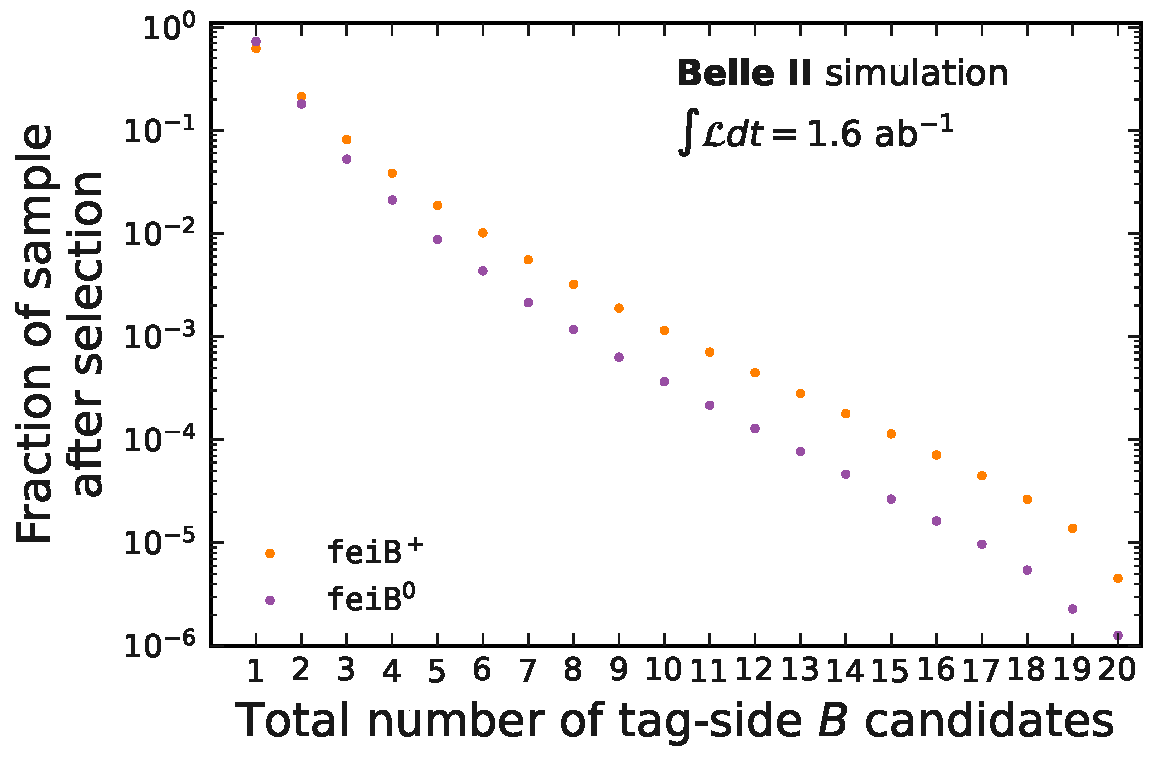
\includegraphics[width=0.45\textwidth]{figures/event_reconstruction/Bboth_total_tag_candidates.pdf}

    \caption{\label{fig:fei_tag_reco_candidates_post_optimisation} 
    Relative fractions of events for the number of \B meson candidates in the generic \MC dataset after the background suppression selections in \Cref{tab:cutflow}.
    This figure can be directly compared with \Cref{fig:fei_tag_reco_candidates}.
    The overall fractions are similar.
    About 67\%(74\%) of events for \Bp and \Bz \FEI modes have only 1 tag-side candidate.
    About 19\%(17\%) of events for \Bp and \Bz \FEI modes have two tag-side candidates and 7\%(5\%) has 3.
    The number of candidates per event reduces quickly, but faster for \Bz modes, with roughly 2\%(1\%) of events having more than 5 candidates for \Bp and \Bz.
    Note that the same event can have a \Bp and \Bz event reconstructed.
    }
\end{figure}

It is clear, however, that even after all selections there may still exist more than one \B meson + photon combination.
The first step in this is a selection of best-tag-candidate per \FEI mode, i.e. the best candidate between \feiBp and \feiBz modes.
While a general approach could be developed, it was observed that at this stage a particular choice of the tag does not influence the resolution or the average value of the spectrum strongly.
This is visualised in \Cref{fig:same_mode_best_tag_selection}.
For both neutral and charged \BtoXsgamma modes the distributions look similar whether the highest-\feiProb candidate is selected in each event, or a random tag-$B$ meson is chosen as the main candidate.
On the other hand, the \Mbc distribution, as expected, has a higher peak for the case when the highest \feiProb candidate is picked in each event.
The latter result for \BtoXsgamma is shown in \Cref{fig:same_mbc_best_tag_selection}.
The figure also includes a similar \Mbc test for the continuum events.

\begin{figure}[htbp!]
    \centering
    \subcaptionbox{\label{fig:bp_same_mode_best_tag_selection}}{
        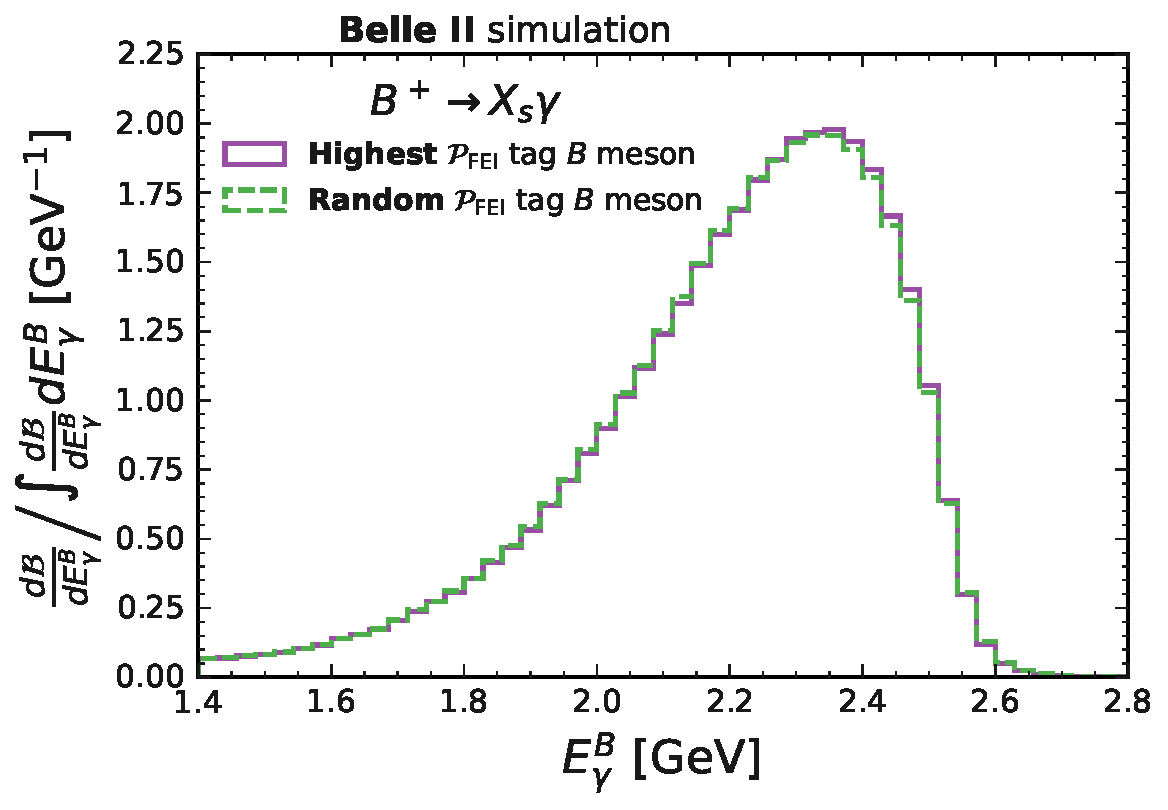
\includegraphics[width=0.4\textwidth]{figures/best_tag_selection/bp_spectrum_with_random_best_tag_selection.pdf}
    }
    \subcaptionbox{\label{fig:bz_same_mode_best_tag_selection}}{
        \includegraphics[width=0.4\textwidth]{figures/best_tag_selection/bp_spectrum_with_random_best_tag_selection.pdf}
    }
    \caption{\label{fig:same_mode_best_tag_selection}Photon energy spectrum (\Cref{fig:bp_same_mode_best_tag_selection}) after selecting a single tag $B$ meson candidate per event either randomly or by requiring the largest \feiProb.
    This is shown for \BptoXsgamma events in \Cref{fig:bp_same_mode_best_tag_selection} 
    and \BztoXsgamma in \Cref{fig:bz_same_mode_best_tag_selection}.
    The figures are normalised to their total integral value such that a shape comparison can be performed.
    Overall, the difference in resolution is small and evaluated at about \order(0.1\%), which is at least an order of magnitude smaller than expected statistical precision of the analysis.
    \todo[inline]{ref resolution chapter}.
    }
\end{figure}

\begin{figure}[htbp!]
    \centering
    \subcaptionbox{\label{fig:bp_mbc_mode_best_tag_selection}}{
        \includegraphics[width=0.4\textwidth]{figures/best_tag_selection/bp_Mbc_with_random_best_tag_selection.pdf}
    }
    \subcaptionbox{\label{fig:bz_mbc_mode_best_tag_selection}}{
        \includegraphics[width=0.4\textwidth]{figures/best_tag_selection/bz_Mbc_with_random_best_tag_selection.pdf}
    }
    \subcaptionbox{\label{fig:bp_continuum_mode_best_tag_selection}}{
        \includegraphics[width=0.4\textwidth]{figures/best_tag_selection/bp_continuum_Mbc_with_random_best_tag_selection.pdf}
    }
    \subcaptionbox{\label{fig:bz_continuum_mode_best_tag_selection}}{
        \includegraphics[width=0.4\textwidth]{figures/best_tag_selection/bz_continuum_Mbc_with_random_best_tag_selection.pdf}
    }
    \caption{\label{fig:same_mbc_best_tag_selection}\Mbc shapes for \BtoXsgamma signal \MC (\Cref{fig:bp_mbc_mode_best_tag_selection,fig:bz_mbc_mode_best_tag_selection}) 
    and \mbox{\epem\ra\qqbar} events from generic-\MC (\Cref{fig:bp_continuum_mode_best_tag_selection,fig:bz_continuum_mode_best_tag_selection}) after selecting a single tag $B$ meson candidate per event either randomly or by requiring the large \feiProb.
    \Cref{fig:bp_mbc_mode_best_tag_selection,fig:bp_continuum_mode_best_tag_selection} show that the difference in the \Mbc distribution for \BptoXsgamma and \BztoXsgamma mostly pronounced in the peak region.
    On the other hand, \Cref{fig:bp_continuum_mode_best_tag_selection,fig:bz_continuum_mode_best_tag_selection} shows not strong dependance in shape irrespective of the way the tag-side candidate is chosen.
    The figures are normalised to their total integral value such that a shape comparison can be performed.
    This observation motivates to selected the highest-\feiProb candidate.
    }    
\end{figure}

As it is desirable to emphasise the contrast between continuum and $B$ events for the fitting step that will follow (see XXX)
\todo[inline]{XXX}
the highest \feiProb candidate in each event is chosen as the $B$ candidate with virtually no bias to the resolution.
However, the study here, as of yet, does not address the cases when there is a candiate in the same event reconstructed in \feiBp and \feiBz.
Therefore, for now, both candidates are kept in such events and the study is continued in \Cref{sec:select_best_candidate}.

\subsection{Selection between \texorpdfstring{\feiBp}{feiB+} and \texorpdfstring{\feiBz}{feiB0} mode}\label{sec:select_best_candidate}

The last section showed that one can select the highest \feiProb candidate from \feiBp and \feiBz without a significant effect on the \EB resolution, and with an enhancement of the \Mbc distribution peak.
As such it reduced each event to a signle tag-$B$ and photon combination in most events.
However, it did not address the case when there is a candidate reconstructed in both \feiBp and \feiBz modes: implying that events may still have up to two combinations.
Such cases are evaluated to happen roughly 10.5\% of time. 
For the sample where two $B$ candidates exist, two quantities are calculated
\begin{equation}\label{eq:asymmetry_tag}
    \mathcal{A}_{\mathrm{tag}} = \frac{\mathcal{P}_{\mathrm{tag}}(\feiBp) - \mathcal{P}_{\mathrm{tag}}(\feiBz)}{\mathcal{P}_{\mathrm{tag}}(\feiBp) + \mathcal{P}_{\mathrm{tag}}(\feiBz)},
\end{equation}
which is called the asymmetry of \feiProb between a \feiBp and \feiBz candidate in the same event, and
\begin{equation}\label{eq:delta_mbc}
    \Delta(\Mbc) = \Mbc(\Bp) - \Mbc(\Bz),
\end{equation}
which is the difference in \Mbc value of the two candidates.
The $\mathcal{A}_{\mathrm{tag}}$ tends to zero if they both have a similar \feiProb and to $\pm$ unity if one of the candidates has a much larger \feiProb.
The second $\Delta(\Mbc)$ is a difference in \Mbc between both of the candidates.
These quantities are visualised in a two-dimensional grid in \Cref{fig:selecting_tag_mode}.
In the figure, the sample is split into two samples, where a real \Bp or \Bz hadronic decay is present on the tag-side, in \Cref{fig:bp_selecting_tag_mode} and \Cref{fig:bz_selecting_tag_mode}, respectively.
If a $\Bp$ candidate is present $\mathcal{A}_{\mathrm{tag}}\approx1$ and $\Delta(\Mbc)\gtrsim 0$ for majority of the candidates.
For $\Bz$ candidates the opposite is true: $\mathcal{A}_{\mathrm{tag}}\approx-1$ and $\Delta(\Mbc)\lesssim 0$ for majority of the candidates.
This result implies that if the true candidate is a \Bp(\Bz), then the value of \feiProb will be higher from \feiBp (\feiBz) candidates the opposite \FEI mode.
Furthermore, the fact that $\Delta(\Mbc)$ tends to be higher can simply be understood that the incorrect candidate is more likely to be present in the tail, rather than peak region of \Mbc.

\begin{figure}[htbp!]
    \centering
    \subcaptionbox{\label{fig:bp_selecting_tag_mode}}{
        \includegraphics[width=0.4\textwidth]{figures/best_tag_selection/Bp_selecting_between_bp_bz.pdf}
    }
    \subcaptionbox{\label{fig:bz_selecting_tag_mode}}{
        \includegraphics[width=0.4\textwidth]{figures/best_tag_selection/Bz_selecting_between_bp_bz.pdf}
    }
    \caption{\label{fig:selecting_tag_mode} A two-dimensional grid of $\mathcal{A}_{\mathrm{tag}}$ (\Cref{eq:asymmetry_tag})
    and $\Delta(\Mbc)$ (\Cref{eq:delta_mbc}) for events that have 2 $B$ candidates from \feiBp and \feiBz modes.
    Candidates with a real tag-side $B^+$ decay (\Cref{fig:bp_selecting_tag_mode})
    and a real tag-side $B^0$ decay (\Cref{fig:bz_selecting_tag_mode}) are shown.
    Most candidates lie near $\mathcal{A}_{\mathrm{tag}}\approx +1 (-1)$ and
    $\Delta(\Mbc)$ value tends to be positive (negative) for $\Bp(\Bz)$ candidates.
    The percentages show the fraction of candidates falling in a given two-dimension bin.
    }
\end{figure}

Based on the observations discussed in this sections, it can be concluded that it is appropriate to select the \FEI candidate with the highest signal probability even when selecting between different \feiBp and \feiBz modes.
This selections finalises the best-candidate selection in this analysis as now it is ensured that every photon candidate corresponds to a single, unique tag-side $B$ meson candidate.

\subsection{Truth-level tag \texorpdfstring{\B}{B} mesons}\label{sec:good_tag_definition}

In particle physics simulation it is possible to rely on the information, provided by the simulation generators to trace back the measured and reconstructed particles all the way to the generated particles.
This procedure is called \textit{truth-matching} and is the usual way to associate `measured-objects' and `generated-objects'.
In particular, the truth-matching requirements ensure that all the particles have correct particle species, momenta, energy determined and, if unstable, the same should be true for their entire decay chain.
This is crucial when performing analysis setup on simulated samples in order to ensure that conclusions, such as efficiency are only drawn from the signal mode samples.
However, in the case of tag $B$ meson reconstruction it is not particularly important to know that the $B$ meson and its entire decay chain is reconstructed fully correctly.
The most important and crucial requirement for a tag is its consistent kinematic constrain that can be provided.
In this analysis a good kinematic constraint manifests as resonant behaviour in \Mbc for the tag-$B$ meson distribution.

Using \texttt{basf2} truth-level information the reconstructed tag-$B$ mesons are subdivided into 11 categories and one or more combinations of the categories based on the differences from the generated decay chains.
The categories are as follows:
\begin{enumerate}
    \setcounter{enumi}{0}
    \item The tag-$B$ and all its daughters are correctly identified and associated;
    \item A final-state radiation photon is not reconstructed;
    \item The tag-$B$ contains more non-final state particles (i.e. resonances) that were not reconstructed;
    \item The tag-$B$ was reconstructed from the secondary decay product which implies that a wrong mass-hypothesis was used;
    \item The tag-$B$ has a missing neutrino;
    \item The tag-$B$ has a photon missing;
    \item The tag-$B$ has a massive final-state particle missing;
    \item The tag-$B$ has a $K_L$ missing (special category compared to 6);
    \item The tag-$B$ has a final state particle associated that has a wrong-signed charged;
    \item The tag-$B$ has a (n-th) daughter non-final-state particle which belongs to a different particle;
    \item Different error in the truth-matching procedure.
\end{enumerate}
Furthermore, all possible combinations between these are created (e.g. The tag-$B$ has a photon \textbf{and} a massive final-state particle missing.)
In total 108 combined categories are observed in the admixture of \BtoXsgamma signal \MC samples for $B$ meson candidates.
Most categories, particularly higher-order combinations, do not have any entries in simulated data samples due to their rareness or kinematic inconsistency.

For every tag-$B$ meson candidate in each signal \MC event, an \Mbc distribution is produced 
and the Jensen-Shannon distance is calculated with respect to category 0 (attributed to perfect reconstruction).
As category 0 (by definition) provides the \textit{best possible kinematic constraint}, the Jensen-Shannon distance is sought to be as close to 0 as possible.
Such a result would imply that the difference of the reconstructed tag-$B$ meson is inconsequential to the quality of the constraint.
As an additional metric, for each category, the fraction of $B$-meson candidates with $\Mbc<5.27~\gevcc$ is evaluated.
In a perfect reconstruction case, this number is practically 0.

The two-dimensional distribution of Jensen-Shannon distances and the fraction of $B$-meson candidates with $\Mbc<5.27~\gevcc$
for all 108 combined categories is shown in \Cref{fig:good_tags_jsdists}.
The figures clearly show that for charged, neutral and admixture of the two, the fraction of $B$-meson candidates with $\Mbc<5.27~\gevcc$ begins to swift;y grow at Jensen-Shannon distance$approx0.3$.
The requirement of Jensen-Shannon distance$<0.3$ is adopted as the threshold to consider a $B$ meson reconstruction category as providing a `good'-kinematic constraint.
Note that the results between different categories are consistent: the same modes are extracted for \Bp, \Bz and the mixture of two.
The modes chosen in this analysis as ones that provide good-kinematic constraint are summarised in \Cref{tab:error_codes}.

\begin{table}[htbp!]
    \centering
    \caption{\label{tab:error_codes}Categories of tag-$B$ reconstruction that provide a 'good' kinematic constraint.
    These categories correspond to the blue points in \Cref{fig:Bboth_good_tags_jsdists}.
    The definitions of each category are provided in \Cref{sec:good_tag_definition}'s text.
    }
    \begin{tabular}{c|c}
    \hline
    Category number    & Jensen-Shannon distance  \\ \hline
    1                  & 0          \\ \hline
    9                & 0.02       \\ \hline
    8                & 0.07       \\ \hline
    9,8                & 0.09       \\ \hline
    3                  & 0.11       \\ \hline
    9,3                & 0.15       \\ \hline
    5                 & 0.19       \\ \hline
    8,3                & 0.21       \\ \hline
    5,3                 & 0.24       \\ \hline
    6                 & 0.24       \\ \hline
    8,5,3                & 0.25       \\ \hline
    9,6                & 0.26       \\ \hline
    9,5                & 0.26       \\ \hline
    8,6                & 0.27       \\ \hline
    6,5                 & 0.27       \\ \hline
    9,5,3                & 0.30       \\ \hline
\end{tabular}
\end{table}

\begin{figure}[htbp!]
    \centering
    \subcaptionbox{\label{fig:Bp_good_tags_jsdists}}{
        \includegraphics[width=0.3\textwidth]{figures/best_tag_selection/Bp_good_tags_definition.pdf}
    }
    \subcaptionbox{\label{fig:Bz_good_tags_jsdists}}{
        \includegraphics[width=0.3\textwidth]{figures/best_tag_selection/Bz_good_tags_definition.pdf}
    }
    \subcaptionbox{\label{fig:Bboth_good_tags_jsdists}}{
        \includegraphics[width=0.3\textwidth]{figures/best_tag_selection/Bboth_good_tags_definition.pdf}
    }
    \caption{\label{fig:good_tags_jsdists} The two-dimensional distribution of Jensen-Shannon distances and the fraction of $B$-meson candidates with $\Mbc<5.27~\gevcc$
    shown for \BptoXsgamma (\Cref{fig:Bp_good_tags_jsdists}), \BztoXsgamma (\Cref{fig:Bz_good_tags_jsdists}), and the mixture of the two (\Cref{fig:Bboth_good_tags_jsdists})
    There are 108 categories in total that have their \Mbc distributions evaluated.
    The legend is shared between the figures.
    The blue dots are chosen as the definition of tags providing a good kinematic constraint (`good' tags).
    The choice is based on a threshold of Jensen-Shannon distance$>0.3$, where it can be seen that fraction of $B$-meson candidates with $\Mbc<5.27~\gevcc$ begins to swiftly grow.
    }
\end{figure}

The \Mbc distribution for \BtoXsgamma admixture with categories providing a `good' kinematic constraint and a `bad' one are shown in \Cref{fig:goodbad_comparison}.
The same figure also highlights the difference if no procedure such as the one described in this section would be introduced.
One can see a large resonant behaviour of non-perfectly reconstructed tags in \Cref{fig:isSig_comparison}, which is mostly absorbed into the definition of a `good' tag provided in this section.
This highlights the importance of the study presented in this chapter -- it would be difficult to separate the non-perfectly reconstructed tag-$B$ meson distribution from the perfectly reconstructed one in an \Mbc fit that will follow (see XXX), due to a large correlation between their shapes.
\todo[inline]{se XXXX}
For the rest of this thesis a tag $B$ meson that provides a `good' kinematic constraint will simply be referred to as a \textit{good} tag.

\begin{figure}[htbp!]
    \centering
    \subcaptionbox{\label{fig:goodbad_comparison}}{
        \includegraphics[width=0.4\textwidth]{figures/best_tag_selection/goodbad_tag_comparison.pdf}
    }
    \subcaptionbox{\label{fig:isSig_comparison}}{
        \includegraphics[width=0.4\textwidth]{figures/best_tag_selection/isSig_tag_comparison.pdf}
    }
    \caption{\label{fig:good_tag_definitions} \Mbc distribution of \BtoXsgamma admixture with split by "good"/"bad" kinematic constrain criterion (\Cref{fig:goodbad_comparison})
    and the conventional perfect/non-perfect reconstruction criterion (\Cref{fig:isSig_comparison}).
    The definition of a tag-$B$ meson that provides a good kinematic constraint described in \Cref{sec:good_tag_definition} is clearly able to describe the resonant-\Mbc structure better.
    \todo[inline]{why are they differently normalised????}
    }
\end{figure}

\section{\texorpdfstring{\Mbc}{Mbc} fitting setup}\label{sec:fitting_mbc}
By this point in the analysis, all the selections have been finalised and discussed.
Furthermore, clear definitions for tag-$B$ mesons that properly kinematically constrain \BtoXsgamma are presented, such that \EB is evaluated accurately.
However, as can be seen in \Cref{fig:spectrum_after_optimisation}, even if continuum and $\BB$ backgrounds are suppressed heavily compared to the initial sample (\Cref{fig:spectrum_after_reco}),
there is still a significantly more background events than \BtoXsgamma signal events.
Many of these, particularly continuum background, originate from incorrect tag-$B$ meson reconstruction (see \Cref{fig:good_tag_definitions}) and can therefore be estimated in data using an \Mbc fitting procedure.
In this Section, a thorough overview of the \Mbc fit is presented which extracts the counts of good tag-$B$ in different \EB intervals.
All fits shown in this Section are unbinned extended negative log-likelihood fits, as presented in \Cref{sec:fitting_theory}.


\subsection{Components in the selected data set}\label{sec:fitting_components}

There are three types of events in the \epem collision data set following all the selections described so far:
\begin{itemize}
    \item Generic \BB (including \BtoXsgamma) that are tagged with a good tag-$B$;
    \item Generic \BB (including \BtoXsgamma) that are tagged with a misreconstructed tag-$B$;
    \item Photon candidates originating in $\epem\ra\qqbar$.
\end{itemize}
These three components are referred to as `peaking', `combinatorial \BB' and `continuum' throughout \Cref{sec:fitting_mbc}.
These components, extracted from generic \MC, are visualised in \Cref{fig:tag_component_fits}.

\begin{figure}[hbtp!]
    \centering
    \subcaptionbox{\label{fig:good_tags_fit}}{
        \includegraphics[width=0.31\textwidth]{figures/fitting/mbc_good_tags_fit.pdf}
    }
    \subcaptionbox{\label{fig:combinatorial_tags_fit}}{
        \includegraphics[width=0.31\textwidth]{figures/fitting/mbc_combinatorial_tags_fit.pdf}

    }
    \subcaptionbox{\label{fig:argus_tags_fit}}{
        \includegraphics[width=0.31\textwidth]{figures/fitting/mbc_continuum_tags_fit.pdf}
    }
    \caption{\label{fig:tag_component_fits} Separate components that are present in generic \MC after selections that suppress background (\Cref{tab:cutflow}).
    The individual components are defined in the text of \Cref{sec:fitting_components}.
    Each distribution contains an unbinned fit to the data points, and the subpanels show the pull (\Cref{eq:pull_distribution}) in each case.
    The fitting function for peaking tag \B mesons (\subref{fig:good_tags_fit}) is chosen as the Crystal Ball function;
    for combinatorial tag \B mesons (\subref{fig:combinatorial_tags_fit}) it is chosen as the 5th order Chebyshev;
    for continuum \epem\ra\qqbar events (\subref{fig:argus_tags_fit}) it is chosen as the ARGUS function.
    }
\end{figure}

The fitting model is prepared to describe the three components and, particularly, to extract the number of tag-$B$ candidates that correspond to the `peaking' component.
The strategy to describe each component is as follows:
\begin{itemize}
    \item Peaking \Mbc distributions are often fitted using a Crystal Ball function.
    It is defined in \Cref{sec:crystal_Ball} and can be understood as a Gaussian distribution with a polynomial tail.
    \Cref{fig:good_tags_fit} illustrates the suitability to describe the peaking \Mbc distribution.
    \item Continuum \Mbc distributions are conventionally described by the ARGUS function designed specifically for continuum events, defined in \Cref{sec:argus_distribution}.
    This function is used to describe $\epem\ra\qqbar$ simulated backgrounds in this analysis and shown in \Cref{fig:argus_tags_fit}.
    \item The particular shape of the combinatorial \BB background is generally dependent on the signal mode and does not have a conventional method of description.
    In this analysis, the usage of \FEI and the fact that background events are conservatively suppressed to avoid signal-side biases lead to a wide but slightly peaking shape.
    Several options were assessed, but it was found to be suitably described by a Chebyshev polynomial, which can be adapted to a necessary functional shape.
    The definition of Chebyshev polynomials is given in \Cref{sec:chebyshev_distribution}.
    A 5th-order polynomial describes the combinatorial \BB background distribution in \Cref{fig:combinatorial_tags_fit},
\end{itemize}
In \Cref{fig:tag_component_fits}, the subpanels show the pull distribution, defined as:
\begin{equation}\label{eq:pull_distribution}
    \mathrm{pull}(x) = \frac{x-\mu}{\sigma}. 
\end{equation}
Throughout this thesis it is used to evaluate the quality of the fit, as repeated measurements of a random variable $x$ should fluctuate around a mean value $\mu$ with a statistical width $\sigma$.
Therefore, any dependencies or structures observed in the pull distribution would be indicators of poor fit quality. 

\subsection{Photon energy intervals for the fit}\label{sec:binning}

It is clear from \Cref{fig:spectrum_after_optimisation} that the signal-to-background ratio changes across all \EB intervals.
Furthermore, even continuum-to-\BB event fractions are not constant.
This is a result of the fact that photons related to \epem\ra\qqbar backgrounds are more likely to extend to high-\EB values because they do not originate from a \B meson which is always produced with an energy $\approx\sqrt{s}/2$ at Belle~II.
The goal of the fit, as discussed in the introduction of this Section, is to remove combinatorial \BB and continuum events from further analysis.
While an overall \Mbc fit could be performed, such an approach necessarily loses event-level information, such as the energies of individual photons, and only provides the event counts in the fitted \EB region.
Moreover, the background composition is expected to vary with \EB, hence such an overall fit may generally be suboptimal.

Instead, in this analysis, the photon spectrum is divided into multiple \EB intervals, and the \Mbc distributions belonging to each interval are fitted using the functions described in \Cref{sec:fitting_components}.
This approach reduces the existing data set to multiple \EB intervals with known good tag-\B counts, completely removing continuum and combinatorial \BB events from the data set.
Such an approach means that the final photon energy spectrum is provided with the same binning as used for fitting.
It is therefore important to optimise the chosen intervals for the fit with respect to the expected \BtoXsgamma signal-to-background ratio, 
even if the primary goal of the fit is not signal extraction.

Three scenarios are tested for $\EB\in(1.4,2.8)~\gev$: 50~\mev, 100~\mev and 200~\mev wide bins.
The test is performed by evaluating the statistical significance, with a definition equivalent to \Cref{eq:soversqrtsplusb}, on a data set scaled to 189~\invfb.
In this case, the background is considered as non-\BtoXsgamma events that remain after the \Mbc fit: only correctly tagged \BB events (no combinatorial or continuum background).
The result of the study of the statistical significance for the hybrid-signal model (\Cref{sec:signal_model}) is shown in \Cref{fig:binning_significance}.

\begin{figure}[hbtp!]
    \centering
    \includegraphics[width=0.5\textwidth]{figures/fitting/binning_significance.pdf}
    \caption{\label{fig:binning_significance}
    The statistical significance based on \Cref{eq:soversqrtsplusb}.
    Here, $S$ is taken as the number of \BtoXsgamma events after fitting and $B$ is taken as non-\BtoXsgamma events expected after fitting in each \EB interval.
    Three scenarios are tested: 50~\mev, 100~\mev and 200~\mev wide bins.
    The final binning chosen is a hybrid scenario described in \Cref{sec:binning}.
    The hybrid model described in \Cref{sec:signal_model} is used for this study.
    }    
\end{figure}

In general, the highest statistical significance is observed with the widest bins, but this method, by definition, contains the least amount of information about the spectrum.
Irrespective of the bin width,  $\EB\in(1.4,1.8)$ and $\EB>2.7~\gev$ show a statistical significance lower than unity, therefore the selected binning should attempt to maximise it.
In the case of $\EB\in(1.9,2.0)~\gev$, it is observed that a similar statistical significance can be achieved in $\EB\in(1.8,2.0)~\gev$.
This motivates choosing the wider bin to achieve a lower threshold than the one in the analysis by BaBar~\cite{BaBar:2007yhb}.
On the other hand, the studies performed in \Cref{sec:resolution_studies} showed that the resolution of \EB is expected to be roughly $30-40~\mev$.
Choosing a fine binning \EB compared to the resolution may lead to complications in the unfolding procedure.
As the simpler bin-by-bin unfolding is employed in this analysis, the 50~\mev bins were not considered.

These considerations led to choosing the following eleven \EB bins for the analysis:
\begin{itemize}
    \item Three 200~\mev bins for $\EB\in(1.4,2.0)~\gev$;
    \item Seven 100~\mev bins for $\EB\in(2.0,2.7)~\gev$;
    \item A single, inclusive overflow bin $\EB>2.7~\gev$.
\end{itemize}
This choice provides a compromise between statistical significance, \EB spectrum resolution and complications in unfolding.
The expected continuum, combinatorial, correctly-tagged non-\BtoXsgamma and correctly-tagged \BtoXsgamma event count expectations for the chosen binning are provided in \Cref{tab:expected_events}.
The Table entry containing combinatorial tag-\B backgrounds may include events where \BtoXsgamma are present.
However, they are rejected as background in the \Mbc fits.
On the other hand, the peaking-\BB background, which is not rejected by the \Mbc fit and treated in \Cref{sec:background_subtraction}, is separated from \BtoXsgamma.
The Table also highlights the importance of a valid binning; several bins can achieve a comparable statistical significance to what could be achieved if just a single bin was used.

\begin{table}[hbtp!]
    \caption{\label{tab:expected_events}
    The expected number of events as a fraction of the data set after selections in \Cref{tab:cutflow}, for the binning chosen in \Cref{sec:binning}.
    The table also shows corresponding statistical significance for a 189~\invfb sized data set.
    }
    \resizebox{1\textwidth}{!}{
\begin{tabular}{|l|lllll|}
\hline
\EB bins [\gev] & Continuum frac. & Combinatorial \BB (incl. \BtoXsgamma) & Peaking \BB frac (excl. \BtoXsgamma) & Peaking \BtoXsgamma & $\frac{S}{\sqrt{S+B}}$ at 189~\invfb \\
\hline
$1.4-1.6$ &    0.22 &       0.20 &   0.047 &  0.00010 & 0.1 \\
$1.6-1.8$ &    0.14 &      0.094 &   0.028 &  0.00031 & 0.38 \\
$1.8-2.0$ &    0.088 &      0.046 &   0.016 &   0.00097 &  1.56 \\
$2.0-2.1$ &   0.028 &      0.013 &  0.0048 &   0.0010 &    2.80 \\
$2.1-2.2$ &    0.020 &     0.0079 &  0.0026 &   0.0016 &  5.05 \\
$2.2-2.3$ &   0.013 &     0.0048 &   0.00093 &   0.0019 &  7.5 \\
$2.3-2.4$ &  0.0075 &     0.0033 &  0.00031 &    0.0019 &   8.4 \\
$2.4-2.5$ &  0.0042 &     0.0019 &  0.00024 &   0.0015 &   7.6 \\
$2.5-2.6$ &  0.0019 &    0.00062 &  0.00013 &    0.0011 &  6.5 \\
$2.6-2.7$ & 0.00059 &    0.000098 & 0.000016 &  0.00014 &  2.38 \\
$2.7-5.0$ & 0.00021 &     0.000011 &   $<0.000001$ &  0.000005 & 0.46 \\
\hline
All        &    0.52 &       0.37 &    0.10 &    0.011     &   6.61 \\
\hline
\end{tabular}
}
\end{table}

Because of the low expected statistical significance, $\EB\in(1.4,1.8)$ and $\EB>2.7~\gev$ are chosen as validation regions.
They are referred to as \textit{sidebands}.
The \textit{signal region} of the analysis is defined as $\EB\in(1.8,2.7)~\gev$.

\subsection{\texorpdfstring{\Mbc}{Mbc} fit model building}\label{sec:fitting_setup}

The functions introduced in \Cref{sec:fitting_components} and \Cref{sec:appendix_fitting_functions} are now considered in terms of the defined binning in \Cref{sec:binning}.
They are used to build an \Mbc fit model for the total data set.
The implementation of an $N$-th order Chebyshev polynomial, a Crystal Ball function and an ARGUS function results
in $N+6$ model parameters and 3 normalisation parameters for each \EB bin.
For fit stability purposes, it is desirable to reduce this number.
Firstly, a primary fit model is prepared, where some of the parameters can be pre-determined or shared amongst the bins.
The key idea is that all the functions are fitted once, separately, on the subsets of the simulated data that they aim to describe.
This also provides the initialisation values of the parameters that are used on the final fit of the total entire data set.
The primary fits for every component are discussed in the following Subsections.

\subsubsection{Crystal Ball primary fit}\label{sec:crystal_ball_prefit}

The Crystal Ball function describes the distribution of peaking tag-\B mesons in \Mbc in terms of shape parameters $\mu$, $\sigma$, $\alpha$ and $n$ and the normalisation of the \PDF, $\mathcal{N}$ (see \Cref{eq:crystal_ball}).
In principle, the reconstruction of the tag-\B meson should not be strongly influenced by the signal-\B meson, which means that the shape parameters should not depend on \EB.
This hypothesis is tested in \Cref{fig:crystal_ball_par_test}.
It can be seen that strong correlations between \EB and parameters $\mu$ and $\sigma$ are absent.
This test is not performed on parameters $\alpha$ and $n$, as they tend to be less stable than $\mu$ and $\sigma$, depending more on the fluctuations of the data set.
It is therefore concluded that a single Crystal Ball shape is sufficient, where all \EB bins share the same shape parameters.
The discussed primary fits are performed simultaneously on the peaking tag-$B$ meson \Mbc distributions in \MC for all \EB bins.
They are shown in \Cref{fig:primary_cb_fits}.
The evaluated shape parameters are fixed for the final \Mbc fit model.
The parameter values and uncertainties from the primary fit are shown in \Cref{tab:fitting_init_params}.

\begin{figure}[hbtp!]
    \centering
    \subcaptionbox{\label{fig:crystal_ball_mus}}{
        \includegraphics[width=0.45\textwidth]{figures/fitting/Crystal_Ball_PDF_test_mu.pdf}
    }
    \subcaptionbox{\label{fig:crystal_ball_sigmas}}{
        \includegraphics[width=0.45\textwidth]{figures/fitting/Crystal_Ball_PDF_test_sigma.pdf}
    }
    \caption{\label{fig:crystal_ball_par_test}The parameters from \Mbc fits of peaking tag-\B mesons in generic \BB simulation, using a Crystal Ball function.
    The datapoints showcase the estimated parameters $\mu$ (\subref{fig:crystal_ball_mus}) and $\sigma$ (\subref{fig:crystal_ball_sigmas}) for different
    \EB intervals.
    This can be compared with the overall shape (blue band), which is determined if the entire $\EB\in(1.4,2.8)~\gev$ region is fitted.
    The parameters of the blue band correspond to the fit in \Cref{fig:good_tags_fit}.
    No strong dependence on \EB is observed.
    }
\end{figure}

\subsubsection{Chebyshev polynomial primary fit}\label{sec:chebyshev_prefit}

The Chebyshev \PDF takes $N$ parameters, $k_i$ ($i=\{1,..N\}$), and a normalisation, $\mathcal{N}$ (\Cref{eq:chebyshev_pdf}).
$N$ is therefore referred to as the \textit{order} of the Chebyshev \PDF.
Third, fourth and fifth order Chebyshev polynomials are tested for suitability to describe the combinatorial \BB background distribution.
The fifth-order result was already introduced in \Cref{fig:combinatorial_tags_fit}.
The results of the best fit for lower-order polynomials are presented in \Cref{fig:lower_order_chebyshev}.
From the pull distributions in the subpanels and the general inspection of the fit, it is clear that using a polynomial of order lower than five is insufficient for an adequate description of combinatorial \BB events.

\begin{figure}[hbtp!]
    \centering
    \subcaptionbox{\label{fig:3rd_order_chebyshev}}{
        \includegraphics[width=0.45\textwidth]{figures/fitting/3rd_order_chebyshev_polynomial.pdf}
    }
    \subcaptionbox{\label{fig:4th_order_chebyshev}}{
        \includegraphics[width=0.45\textwidth]{figures/fitting/4th_order_chebyshev_polynomial.pdf}
    }
    \caption{\label{fig:lower_order_chebyshev}The \Mbc fits of combinatorial \BB events with a third-order~(\subref{fig:3rd_order_chebyshev}) or fourth-order~(\subref{fig:4th_order_chebyshev}) Chebyshev \PDF.
    These Figures can be compared to \Cref{fig:combinatorial_tags_fit}.
    Lower-order Chebyshev polynomials are unable to accurately describe the combinatorial \BB data.
    }
\end{figure}


The coefficients $k_{1-5}$ of the Chebyshev polynomial cannot be easily connected to physical observables,
and therefore it is hard to evaluate their dependence on \EB.
As such, three different Chebyshev PDFs are evaluated for the following intervals: $\EB\in(1.4,1.6)$, $\EB\in(1.6,1.8)$, $\EB>1.8$ \gev.
The last interval is not subdivided further because of the data set size (see \Cref{tab:expected_events}), each interval is optimised to contain an approximately equal expected number of events.
The discussed primary fits are performed simultaneously on the \Mbc distributions of the combinatorial \BB in all \EB bins.
They are shown in \Cref{fig:primary_cheb_fits}.
The determined coefficients $k_{1-5}$ are fixed for the final \Mbc fit model.
The primary fit values are presented in \Cref{tab:fitting_init_params}.

\subsubsection{ARGUS primary fit}\label{sec:argus_prefit}

Similarly to the previous cases, the ARGUS function has 2 parameters, $c$ and $m_0$, and a normalisation $\mathcal{N}$ (\Cref{eq:argus_function}).
Unlike the coefficients of the Chebyshev, $c$ and $m_0$ are easier to understand intuitively: with $m_0$ corresponding to the maximum allowed \Mbc values in the distribution and $c$ to the shape of continuum background.
More generally, the variation of $c$ and $m_0$ accounts for possible background shape differences between \MC and data.
It offers an additional layer of flexibility through a variation of relative ARGUS and Chebyshev normalisation values.
This means that allowing a degree of variation in the ARGUS shape is beneficial to account for possible background differences in data.

Following these considerations, a setup is adopted with independent shapes for  \mbox{$\EB\in(1.4,1.6)$~\gev}, \mbox{$\EB\in(1.6,1.8)$~\gev}, $\EB>1.8$~\gev.
In each respective range, one single shape parameter $c^{(1.4-1.6)}$, $c^{(1.6-1.8)}$, $c^{(>1.8)}$ is determined from the total fit.
To account for possible differences between simulated and data $\sqrt{s}$, the $m_0$ parameter is shared between all bins and is also determined from the fit of the combined data set.
The discussed primary fits are performed simultaneously on continuum \Mbc distributions in all \EB bins.
They are shown in \Cref{fig:primary_argus_fits}.
The initial values for the final \Mbc fit model are presented in \Cref{tab:fitting_init_params}.

\subsubsection{Final fit model}

Based on the primary fits of the subcomponents of the total data set, the number of fitting parameters is reduced:
certain fit parameters are shared between different \EB intervals, whereas other parameters are kept at their initialised value and not varied.
The final \Mbc fitting model for the analysis is summarised in \Cref{tab:fitting_init_params}.
It shows the initial values for each parameter and highlights which parameters are kept fixed in the final \Mbc fit.
It can be seen, that the previously introduced $11\cdot(5+2+4+3)=154$ parameters are reduced to $37$ fitting parameters.
The fitting model is then applied to the total data set in \Cref{sec:mbc_fit_full_mc} 
in order to estimate the main parameter of interest: 
normalisations of the Crystal Ball in every \EB bin (i.e. the number of good tag-$B$ in each \EB bin).
The primary \Mbc fits determining the parameters in 
\Cref{tab:fitting_init_params} on corresponding data sets are given in \Cref{sec:appendix_primary_fits}. 
\begin{table}[hbtp!]
    \centering
    \caption{\label{tab:fitting_init_params} 
    The summary of the fitting model used in this analysis for the \Mbc fit.
    For the final \Mbc fit, the parameters are initialised at the values that are listed, corresponding to the ones determined in the primary fitting steps, explained in \Cref{sec:crystal_ball_prefit,sec:chebyshev_prefit,sec:argus_prefit}.
    The values that are bolded in the Table are not estimated from the final \Mbc fit but are kept at their initialised values.
    On the other hand, all non-bolded values can vary in the final fit.
    Uncertainties are evaluated using the \texttt{HESSE} method in the primary fitting steps.
    In the Table, they are omitted if the relative uncertainty is lower than $0.1\%$.
    }
\resizebox{1\textwidth}{!}{
    {\def\arraystretch{1.5}\tabcolsep=5pt
        \begin{tabular}{|c|c|c|c|c|c|c|c|c|c|c|c|}

            \multicolumn{12}{c}{Fitting model} \\
            \hline
            \multirow{2}{*}{\EB bin} & \multicolumn{4}{|c|}{Crystal Ball} & \multicolumn{5}{c|}{Chebyshev}    & \multicolumn{2}{c|}{Argus} \\
            \cline{2-12}
                                    & $\mu$ & $\sigma$ & $\alpha$ & $n$    & $k_1$ & $k_2$ & $k_3$ & $k_4$ & $k_5$ & $c$ & $m_0$                 \\
            \hline
            1.4 -- 1.6               & \multirow{11}{*}{$5.27946\pm0.00002$} & \multirow{11}{*}{$0.00302\pm0.00002$} & \multirow{11}{*}{$1.573\pm0.035$} & \multirow{11}{*}{$3.568\pm0.22$} & $-0.0751\pm0.0071$ & $-0.3125\pm0.0073$ & $-0.2516\pm0.0064$ & $-0.1381\pm0.0064$  & $-0.0296\pm0.0062$  &  $-33.11 \pm    0.79$ & \multirow{11}{*}{$5.2897719 \pm 0.0000006$} \\
            \cline{1-1}\cline{6-11}
            1.6 -- 1.8               &                                      &                                        &                                   &                                  & $-0.01 \pm 0.01$ & $-0.33\pm0.01$ & $-0.283 \pm  0.009$ & $-0.143\pm0.009$ & $-0.033\pm0.009$ & $-28.03 \pm 1.00$ & \\               
            \cline{1-1}\cline{6-11}
            1.8 -- 2.0               &                                      &                                        &                                   &                                  & \multirow{9}{*}{$0.119\pm0.011$} & \multirow{9}{*}{$-0.362\pm0.012$} & \multirow{9}{*}{$-0.348\pm 0.010$} & \multirow{9}{*}{$-0.193\pm0.010$} & \multirow{9}{*}{$-0.029 \pm 0.010$} & \multirow{9}{*}{$-25.07 \pm 0.92$} & \\                         
            \cline{1-1}
            2.0 -- 2.1               &                                      &                                        &                                   &                                  &                 &                  &                   &                  &                    &                   & \\                                                                  
            \cline{1-1}
            2.1 -- 2.2               &                                      &                                        &                                   &                                  &                 &                  &                   &                  &                    &                   & \\   
            \cline{1-1}
            2.2 -- 2.3               &                                      &                                        &                                   &                                  &                 &                  &                   &                  &                    &                   & \\   
            \cline{1-1}
            2.3 -- 2.4               &                                      &                                        &                                   &                                  &                 &                  &                   &                  &                    &                   & \\   
            \cline{1-1}
            2.4 -- 2.5               &                                      &                                        &                                   &                                  &                 &                  &                   &                  &                    &                   & \\   
            \cline{1-1}
            2.5 -- 2.6               &                                      &                                        &                                   &                                  &                 &                  &                   &                  &                    &                   & \\   
            \cline{1-1}
            2.6 -- 2.7               &                                      &                                        &                                   &                                  &                 &                  &                   &                  &                    &                   & \\   
            \cline{1-1}
            2.7 -- 5.0               &                                      &                                        &                                   &                                  &                 &                  &                   &                  &                    &                   & \\   
            \hline
        \end{tabular}
    }
}

\end{table}

\subsection{\texorpdfstring{\Mbc}{Mbc} fit on the total simulated data set}\label{sec:mbc_fit_full_mc}

The prepared fit, discussed in \Cref{sec:fitting_setup}, is applied to the total generic \MC data set.
The initial values of the fit are given in \Cref{tab:fitting_init_params} and all bins are fitted simultaneously.
The fit results are shown in \Cref{fig:primary_full_fits}.
The overall \Mbc distributions are accurately described for all \EB bins, irrespective of the overall number of data points that are being fitted.
This is already an important achievement: a single fitting setup is adaptive enough to cover different signal-to-background ratios, statistical sample sizes and overall shapes of the distributions.
\begin{figure}[hbtp!]
    \centering
    \subcaptionbox{\label{fig:mbc_full_1p4}}{
        \includegraphics[width=0.3\textwidth]{figures/fitting/fits/full_MbcFit_1p4to1p6ppdf.pdf}
    }
    \subcaptionbox{\label{fig:mbc_full_1p6}}{
        \includegraphics[width=0.3\textwidth]{figures/fitting/fits/full_MbcFit_1p6to1p8ppdf.pdf}
    }
    \subcaptionbox{\label{fig:mbc_full_1p8}}{
        \includegraphics[width=0.3\textwidth]{figures/fitting/fits/full_MbcFit_1p8to2p0ppdf.pdf}
    }
    \subcaptionbox{\label{fig:mbc_full_2p0}}{
        \includegraphics[width=0.3\textwidth]{figures/fitting/fits/full_MbcFit_2p0to2p1ppdf.pdf}
    }
    \subcaptionbox{\label{fig:mbc_full_2p1}}{
        \includegraphics[width=0.3\textwidth]{figures/fitting/fits/full_MbcFit_2p1to2p2ppdf.pdf}
    }
    \subcaptionbox{\label{fig:mbc_full_2p2}}{
        \includegraphics[width=0.3\textwidth]{figures/fitting/fits/full_MbcFit_2p2to2p3ppdf.pdf}
    }
    \subcaptionbox{\label{fig:mbc_full_2p3}}{
        \includegraphics[width=0.3\textwidth]{figures/fitting/fits/full_MbcFit_2p3to2p4ppdf.pdf}
    }
    \subcaptionbox{\label{fig:mbc_full_2p4}}{
        \includegraphics[width=0.3\textwidth]{figures/fitting/fits/full_MbcFit_2p4to2p5ppdf.pdf}
    }
    \subcaptionbox{\label{fig:mbc_full_2p5}}{
        \includegraphics[width=0.3\textwidth]{figures/fitting/fits/full_MbcFit_2p5to2p6ppdf.pdf}
    }
    \subcaptionbox{\label{fig:mbc_full_2p6}}{
        \includegraphics[width=0.3\textwidth]{figures/fitting/fits/full_MbcFit_2p6to2p7ppdf.pdf}
    }
    \subcaptionbox{\label{fig:mbc_full_2p7}}{
        \includegraphics[width=0.3\textwidth]{figures/fitting/fits/full_MbcFit_2p7to5p0ppdf.pdf}
    }
    \subcaptionbox{\label{fig:legend}}{
        \includegraphics[width=0.25\textwidth]{figures/fitting/legend.png}
    }
    \caption{\label{fig:primary_full_fits}The fits of the $1.6~\invab$ data set of generic \MC, using the fitting model from \Cref{tab:fitting_init_params}.
    A good description of the \Mbc distributions can be seen throughout the \EB bins.
    This highlights that the fit setup accurately describes large simulated data samples.
    The legend is shown in (\subref{fig:legend}).
    For the rest of the thesis, this legend is always implied for \Mbc fits.
    }
\end{figure}

As was already mentioned, the main goal of the \Mbc fit introduced in this Section is to extract the good tag-\B counts in each \EB bin.
This is equivalent to the normalisation parameter of the Crystal Ball \PDF, $\mathcal{N}_{\mathrm{CB}}$.
These normalisations are shown in \Cref{fig:generic_mc_fit_yield_comparisons}.
The exact values of the rest of the parameters are not needed for further analysis, as long as an unbiased and accurate description of good tag-\B counts is achieved through $\mathcal{N}_{\mathrm{CB}}$.
The main goal of keeping them as free parameters in the fit is to ensure that the \Mbc background shape and yield estimations are sufficiently flexible to account for potential data-simulation discrepancies.
Therefore, for the rest of the thesis, other parameters will not be explicitly mentioned, unless their values are relevant to the discussion.

To ensure that the fit is receptive to changes of \BtoXsgamma signal, two simple tests are devised, where the fit is performed on generic \MC but
\begin{itemize}
    \item all \BtoXsgamma signal events are removed;
    \item \BtoXsgamma signal shape in generic \MC is reweighted using the hybrid model weights.
\end{itemize}
The results are shown in \Cref{fig:no_bxsgamma_mc_fit_yield_comparisons,fig:weighted_mc_fit_yield_comparisons}.
It is clear that if the \BtoXsgamma events are completely removed or reweighted, the \Mbc fit presented in this Subsection responds appropriately.
Therefore, although a particular simulation model was used when preparing the fit, no particular bias towards any \BtoXsgamma model is introduced.

\begin{figure}[hbtp!]
    \subcaptionbox{\label{fig:generic_mc_fit_yield_comparisons}}{
        \includegraphics[width=0.3\textwidth]{figures/fitting/normal_full_fit.pdf}
    }
    \subcaptionbox{\label{fig:no_bxsgamma_mc_fit_yield_comparisons}}{
        \includegraphics[width=0.3\textwidth]{figures/fitting/removed_xsgamma_full_fit.pdf}
    }
    \subcaptionbox{\label{fig:weighted_mc_fit_yield_comparisons}}{
        \includegraphics[width=0.3\textwidth]{figures/fitting/hybrid_weighted_full_fit.pdf}
    }
    \caption{\label{fig:mc_fit_yield_comparisons}The comparisons of estimated peaking tag-\B counts in each \EB bin, $\mathcal{N}_{\mathrm{CB}}$,
    for the total 1.6~\invab generic~\MC data set (\subref{fig:generic_mc_fit_yield_comparisons}).
    Additionally, results are shown for the fits on the generic \MC data set but with all \BtoXsgamma events removed (\subref{fig:no_bxsgamma_mc_fit_yield_comparisons}),
    and for generic \MC data set but with the hybrid-signal model reweighting introduced (\subref{fig:weighted_mc_fit_yield_comparisons}).
    In each case, the uncertainties are $\texttt{HESSE}$ uncertainties estimated by the fit.
    It can be seen that the fit is receptive to the expected count of peaking tag-$B$ mesons.
    Larger uncertainties in (\subref{fig:weighted_mc_fit_yield_comparisons}) are due to known issues in weighted error estimation.
    They do not affect this analysis as weighted fits are not performed later.
    }
\end{figure}

\section{Remaining \texorpdfstring{\BB}{BB} background subtraction}\label{sec:background_subtraction}
After the fitting procedure introduced in \Cref{sec:fitting_mbc} the good tag-\B counts are estimated, and in particular:
\begin{itemize}
    \item all \epem\ra\qqbar contribution has now been removed;
    \item events where the tag-side \B mesons are not properly reconstructed have been removed.
\end{itemize}

However, it may seem odd that after performing the \Mbc fit (see \Cref{fig:mc_fit_yield_comparisons}), the result is still not quite comparable to an \EB spectrum,
and resembles that of the background seen in, e.g., \Cref{fig:spectrum_after_optimisation}.
Due to the fact that in the `inclusive' treatment the $X_s$ is not constrained, a component of \textit{irreducible} background will always be present.
In the case of this analysis the good tag-\B counts after the optimal selection in \Cref{tab:cutflow} and fitting procedure presented here contain:
\begin{itemize}
    \item correctly tagged \BtoXsgamma events,
    \item correctly tagged-\BB events other than \BtoXsgamma.
\end{itemize}
Although in the later iterations of this analysis it may be possible to further diminish the second background component through more complicated selection and fitting procedures, 
some irreducible background component will always remain (see discussion).
\todo[inline]{further discussion, refer to discussuin chapter}

The final step before the full \BtoXsgamma spectrum extraction on simulation is evaluating the size of the remaining \BB background.
Two strategies are considered:
\begin{itemize}
    \item Count good tag-\B mesons in each event that correspond to non-\BtoXsgamma in simulation, and use this value to subtract remaining-\BB events from data.
    This effectively corresponds to the red histograms in \Cref{fig:mc_fit_yield_comparisons}.
    \item Perform the fit again on the simualted sample with \BtoXsgamma events removed.
    This way, good-tag \B meson counts are estimated with fitting effects included.
    This effectively corresponds to the data points in \Cref{fig:no_bxsgamma_mc_fit_yield_comparisons}.
\end{itemize}
Although both choices are valid and have certain advantages, in this analysis, the second method is chosen.
The main reason for this choice is the fact that biases or systematic effects, if such exist, could be suppressed in the fitter when subtracting.
It also requires a similar validation procedure (e.g. to be an unbiased estimator) as the total fit.
Therefore, after the \Mbc fit, the number of good-tagged \BtoXsgamma events in data will be measured as follows:
\begin{equation}\label{eq:background_subtraction}
    \mathcal{N}_{\mathrm{DATA}}^{\BtoXsgamma} = \mathcal{N}_{\mathrm{DATA}}^{\mathrm{good~tags}}  - \frac{189~\invfb}{1600~\invfb} \mathcal{N}_{\mathrm{MC}}^{\mathrm{good~tags~with~\BtoXsgamma~removed}}.
\end{equation}

\section{Analysis strategy validation in simulation}\label{sec:MC_validation}
\Cref{sec:fitting_mbc,sec:background_subtraction} introduced the fitting procedure and \BB background subtraction.
Together with the optimal selections from \Cref{sec:final_optimisation}, this fully defines the analysis strategy from the Belle~II simulated datasets to the \BtoXsgamma spectrum.
However, the defined fitter has to be validated in simulation to give an unbiased estimation of \BtoXsgamma events, with a good resoltion and signal efficiency.
The studies in this Section will show such results.

\subsection{Validation of \texorpdfstring{\Mbc}{Mbc} fit on reduced samble size}\label{sec:mbc_fit_validation_misreconstructed}

The results that were shown in \Cref{fig:mc_fit_yield_comparisons} only provided results for fitting 1.6~\invab -- a dataset about an order of magnitude larger than is expected in the case of this analysis.
Therefore, the generic \MC dataset is pseudorandomly split into 10 smaller subsets, corresponding to 160~\invfb, and each of them are fitted independently.
The choice of 160~\invfb, rather than 190~\invfb which is the sample size of the Belle~II data used in the analysis, is due to anticipated data-simulation differences.
\todo[inline]{see XXX and next paragraph performed where?}
Indeed, a 190~\invfb dataset should correspond to roughly 160~\invfb in simulation due to differences in tag-\B reconstruction efficiency.

The resulting 10 fits and the estimated $\mathcal{N}_{CB}$ corresponding to each \EB bin are shown in \Cref{fig:extracted_validation_mc}.
The expected number of events in each fit is always equal to one tenth of that in the total generic \MC dataset.
It can be observed that all data points, and their average, are statistically compatible with the expectation.
These results indicate, that despite using a 10 times larger dataset to define the \PDF{s}, this \Mbc fit model produces reliable results.
Further tests, particularly a test ensuring that the fitter is unbiased, are performed later.

\begin{figure}[htbp!]
    \includegraphics[width=0.9\textwidth]{figures/mc_validation/extracted_signal_generic_mc.pdf}
    \caption{\label{fig:extracted_validation_mc}The estimated $\mathcal{N}_{CB}$ values from fits on one tenth of generic \MC, corresponding to 160~\invfb of simulation.
    The dashed lines represent different \EB bins, each bin showing one data point corresponding to a simultaneous fit of all \EB bins.
    The dotted lines show the average of all 10 points in each bin, whereas the full lines show the number of good tag-\B events in the original 1.6~\invab dataset, scaled down 10 times (`expected').
    The subpanels show the pull of each datapoint from the expected number of events.
    These results show that the fit is able to extract a result on a dataset that is an order of magnitude smaller.
    }
\end{figure}

\subsection{Validation of subtraction of remaining-\texorpdfstring{\BB}{BB} background}\label{sec:background_subtraction_validation_mc}

The strategy to extract the \BtoXsgamma photon energy spectrum and suppress the remaining \BB background was laid out in \Cref{sec:background_subtraction}.
In particular, full generic \MC dataset is modified, such that no-\BtoXsgamma events are present in it.
Then, the \Mbc fit discussed in \Cref{sec:fitting_setup} is performed.
To test that this procedure is viable, the subtraction is performed for the results shown in \Cref{fig:extracted_validation_mc}.
Although the 10 fits are performed on 160~\invfb datasets, the background subtraction is done with a 1.6~\invab dataset.
Therefore, the statistical uncertainty from the fit on the smaller dataset is dominating.
The subtracted result is shown in \Cref{fig:subtracted_validation_mc}.

\begin{figure}[htbp!]
    \includegraphics[width=0.9\textwidth]{figures/mc_validation/subtracted_signal_generic_mc.pdf}
    \caption{\label{fig:subtracted_validation_mc}
    The estimated $\mathcal{N}_{CB}$ with subtracted background, based on the \Cref{eq:background_subtraction}.
    The values before \BB-background subtraction are shown in a corresponding \Cref{fig:extracted_validation_mc}.
    To ensure that a minimal statistical background subtraction uncertainty is introduced, the full 1.6~\invab dataset is chosen to subtract the background.
    The uncertainties of each data point are those of the \Mbc fit on the background dataset and on the tested subset, added in quadrature.
    }
\end{figure}

The 1.6~\invab dataset and the 160~\invfb subsets are largely correlated, therefore the result has a smaller spread than one might expect from a unit Gaussian, based on the statistical ucnertainty provided by the fitter.
However, the purpose of this test is to showcase that the setup is able to extract values that are statistically compatible with the original dataset.
The results showcased in \Cref{fig:extracted_validation_mc,fig:subtracted_validation_mc} clearly show that the central values of the \EB spectrum extracted follow the number of \BtoXsgamma events in the dataset.
In this section so far, no particular modelling of \BtoXsgamma spectrm has been assumed.
In fact, following the tests from \Cref{fig:mc_fit_yield_comparisons}, it is clear that the analysis is \textit{so far} signal-model independent, as no direct assumptions have been made thus far.
On the other hand, following the setup that is taken to remove \BB backgrounds after the \Mbc fit, the analysis is heavily background-model dependent.
For this reason, special emphasis will be put on testing the \textit{background} description validation, as opposed to signal validation in later chapters XXXX.
\todo[inline]{later chapter xxxx}

\subsection{Closure test of the \texorpdfstring{\Mbc}{Mbc} fitter}\label{sec:closure_test}

If the uncertainties estimated by a fitter are correct, then fitting pseudodata sets generated from \PDF{s} fitted on test data must yield statistically compatible results.
This verifies two important aspects of the fitter:
\begin{itemize}
    \item the estimated parameter central values of the fitter are reproduced, when fitting a statistically equivalent dataset;
    \item the estimated parameter central values of the fitter are distributed accordingly to the uncertainties that the fitter provides.
\end{itemize}

More concisely, the pull distribution of an unbiased fitter, in this case calculated as:
\begin{equation}\label{eq:toy_pull}
    \mathrm{pull} = \frac{\mathcal{N}\times \mathrm{scale} - \mathcal{N}^{\mathrm{pseudo}}}{\mathrm{fit~error}},
\end{equation}
must be described by a unit Gaussian (assuming the central limit theorem is applicable for the psuedodata sample size).
In the case of this analysis, $\mathcal{N}_{\mathrm{CB}}$ is the estimated number of good tag-\B mesons in the generic-\MC sample.
The uncertainty, $\mathrm{fit~error}$ is a corresponding uncertainty, in this analysis estimated by the \texttt{HESSE} method.
On the other hand, $\mathcal{N}^{\mathrm{pseudo}}_{\mathrm{CB}}$ is a randomly sampled dataset that follows the \PDF{s} fitted on the generic-\MC dataset.
The $\mathrm{scale}$ is used to equate the sample size between the sampled and total simulated dataset.
Tests of this type are known as \textit{closure tests} is statistics and allow to verify that the central values reproduced by the fitter fluctuate as indicated by the \PDF uncertainties.

The closure test in this analysis is done on pseudodata sets of equivalent size as the Belle II collected data.
First, 1000 pseudodata sets equivalent to $\mathrm{160~\invfb}$ are sampled from the \PDF that was fitted in \Cref{fig:primary_full_fits}.
Since in all of the cases $\mathcal{N}_{\mathrm{CB}}$ and $\mathrm{fit~error}$ are known exactly, the \Mbc fitter is used on the pseudodata set, and a $\mathrm{pull}$ is calculated based on \Cref{eq:toy_pull}.
The pull distribution for every \EB bin are shown in XXX.
To test the statistical validity of \Mbc fits on each bin, a Gaussian \PDF is fitted on the distributions, with parameters $\mu$ and $\sigma$ being estimated.
The parameters correspond to the mean value, and the width of the Gaussian distribution, respectively.
The parameter estimation is performed as an unbinned negative log-likelihood fit.
The corresponding Gaussian fit result, and the parameters are also shown in XXX.


\section{Simulation-to-data corrections}\label{sec:corrections}
The fitter and background subtraction procedure, introduced in \Cref{sec:fitting_setup,sec:background_subtraction},
have been thoroughly validated in \Cref{sec:MC_validation} in \MC.
The real challenge, as usual, is ensuring that the conclusions and results observed in \MC generalise correctly to real Belle~II data.
The key concept of a blinded analysis dictates that one must validate the analysis procedure in control samples or regions: collections of data that are abundant, well-understood and provide insight into the behaviour of signal in the detector.
In this Section, the discussion about \FEI validation, 
\piz and $\eta$ veto validation, photon detection efficiency and background modelling is presented.
The combined results from all Sections are shown in \Cref{tab:correction_table}.

\begin{table}[htbp!]
    \centering
    \caption{\label{tab:correction_table} The corrections for background (and signal in \Cref{sec:validation_efficiency}) efficiency in the hadronic-tagged \BtoXsgamma photon energy spectrum measurement.
    \FEI calibration calculations are discussed in \Cref{sec:fei_calibration}.
    Derivation of correction for the \piz and $\eta$ veto are presented in \Cref{sec:piz_eta_calibration}.
    The photon detection efficiency study is described in \Cref{sec:photon_efficiency}.
    Background modelling corrections are calculated in \Cref{sec:remaining_bb_background_modelling}.
    The \FEI, \piz and \g corrections are averaged values corresponding to the respective \EB bin,
    as the event-level information is lost after estimating good tag-\B counts using the \Mbc fit and performing the leftover \BB background subtraction.
    }
    \resizebox{1\textwidth}{!}{
    \begin{tabular}{cccc}
        \hline
        {} \EB, GeV  & FEI calibration & \piz veto correction & \g efficiency correction\\
        \hline
        1.4-1.6  &  \multirow{11}{*}{$0.6630 \pm 0.0229$} & $1.090 \pm 0.050$ & $0.991 \pm 0.023$ \\
        1.6-1.8  &                                        & $1.074 \pm 0.048$ & $0.995 \pm 0.022$ \\
        1.8-2.0  &                                        & $1.064 \pm 0.046$ & $0.996 \pm 0.021$ \\
        2.0-2.1  &                                        & $1.055 \pm 0.046$ & $0.996 \pm 0.021$ \\
        2.1-2.2  &                                        & $1.050 \pm 0.047$ & $0.997 \pm 0.021$ \\
        2.2-2.3  &                                        & $1.046 \pm 0.047$ & $0.997 \pm 0.021$ \\
        2.3-2.4  &                                        & $1.045 \pm 0.047$ & $1.000 \pm 0.020$ \\
        2.4-2.5  &                                        & $1.047 \pm 0.047$ & $1.001 \pm 0.019$ \\
        2.5-2.6  &                                        & $1.050 \pm 0.047$ & $1.001 \pm 0.019$ \\
        2.6-2.7  &                                        & $1.050 \pm 0.046$ & $0.998 \pm 0.019$ \\
        2.7-     &                                        & $1.053 \pm 0.046$ & $0.998 \pm 0.018$ \\
        \hline
        \end{tabular}
}


\end{table}


\subsection{Calibration of the \texorpdfstring{\FEI}{FEI} algorithm}\label{sec:fei_calibration}

The working principle of \FEI has already been discussed in \Cref{sec:tag_reconstruction}.
It combines many classifiers which perform reconstructions in various decay chains of the hadronic decays of \B mesons.
Furthermore, the training of the algorithm happens in \MC.
To ensure that the algorithm appropriately acts on Belle~II data, its performance must be studied or \textit{calibrated}.
The calibration study is performed on data collected by the Belle~II, for every simulation campaign, and the work is not part of the original work presented in this thesis.
Full details of the calibration method are presented in Ref.~\cite{Belle-II:2020fst}, but the main details that are relevant to the work of the thesis are summarised here.

The calibration study uses $B\rightarrow X_{u/c} \ell \nu$ decays due to the branching fraction of almost 20~\% and a clean experimental signature, 
where $X_{u/c}$ denotes an inclusive state originating from the $c$ or $u$ quark, similarly to the $X_{s/d}$ notation.
Firstly, in each event, only the highest \FEI probability tag-\B candidate is selected with loose requirements on Fox-Wolfram moments (see \Cref{sec:fox_wolfram_moments}) and $\Delta E$ to ensure adequate \epem\ra\qqbar suppression.
Next, a high energy lepton $p_{\ell}^B>1~\gevc$ is required in each event.
This lepton candidate is required to originate near the interaction point and its identification information from all sub-detectors is required to be consistent with a lepton.

After the selection, a binned likelihood fit for \Mbc is set up, which contains three binned \PDF{s}: signal $B\rightarrow X_{u/c}\ell\nu$ decays, 
secondary or misidentified leptons, and \epem\ra\qqbar events. 
Here, secondary leptons identify leptons coming from the $B$ mesons other than $B\rightarrow X_{u,c}\ell\nu$ decay.
Misidentified leptons are used as a broad term for hadrons whose identification information is consistent with that of either an electron or a muon.
The signal $B\rightarrow X_{u/c}\ell\nu$ \PDF is composed of four sub-\PDF{s}, particularly: $B\rightarrow D\ell\nu$, $B\rightarrow D^*\ell\nu$, $B\rightarrow X_u\ell\nu$ and the rest of  $B\rightarrow X_c\ell\nu$ modes.
The fit is performed separately for the following combinations of tag-\B mesons and lepton:
\begin{itemize}
    \item $B^+$ and $e^-$,
    \item $B^+$ and $\mu^-$,
    \item $B^0$ and $e^-$,
    \item $B^0$ and $\mu^-$.
\end{itemize}
This is shown in \Cref{fig:fei_calib}.
\begin{figure}[htbp!]
    \centering
    \subcaptionbox{\label{fig:fei_calib_bpluseminus}}{
        \clipbox*{{0\width} {0.5\height} {0.5\width} {1\height}}{%
            \includegraphics[width=0.9\textwidth]{figures/data_sim_corrections/tag_calibration.png}
        }
    }
    \subcaptionbox{\label{fig:fei_calib_bplusmuminus}}{
        \clipbox*{{0.5\width} {0.5\height} {1\width} {1\height}}{%
            \includegraphics[width=0.9\textwidth]{figures/data_sim_corrections/tag_calibration.png}
        }
    }
    \subcaptionbox{\label{fig:fei_calib_bzeroeminus}}{
        \clipbox*{{0\width} {0\height} {0.5\width} {0.5\height}}{%
            \includegraphics[width=0.9\textwidth]{figures/data_sim_corrections/tag_calibration.png}
        }
    }
    \subcaptionbox{\label{fig:fei_calib_bzeromuminus}}{
        \clipbox*{{0.5\width} {0\height} {1\width} {0.5\height}}{%
            \includegraphics[width=0.9\textwidth]{figures/data_sim_corrections/tag_calibration.png}
        }
    }
    \caption{\label{fig:fei_calib} Illustration of the fits to \B\to$X_{u/c}\ell\nu$ decays in the \FEI calibration study.
    Results for the combinations of charged and neutral tag-$B$ modes with $e^-$ and $\mu^-$
    are shown in \Cref{fig:fei_calib_bpluseminus,fig:fei_calib_bplusmuminus,fig:fei_calib_bzeroeminus,fig:fei_calib_bzeromuminus}.
    Different fit components are shown in the legend and the subpanels contain the pulls of the fit.
    Figures are taken from Ref.~\cite{Belle-II:2020fst}.
    }
\end{figure}

The branching fractions of $B\rightarrow X_{u/c}\ell\nu$ are evaluated from the fitted distributions.
These values are then directly compared with the experimentally known values of branching fractions of the respective decays.
A correction factor, $\mathcal{C}_{\mathrm{FEI}}$, is derived such that the two values are compatible.
The leading evaluated systematic uncertainties come from the imperfect experimental knowledge of the $B\rightarrow X_u\ell\nu$ branching fractions and their form factors, the fit model composition, tracking and particle identification uncertainties.
For the Belle II simulation campaign used in this analysis, and averaged for both lepton modes, the result is as follows:
\begin{equation}\label{eq:fei_calibration}
    \mathcal{C}_{\mathrm{FEI}}(B^+) = 0.6599 \pm 0.225; \quad \mathcal{C}_{\mathrm{FEI}}(B^0) = 0.6695 \pm 0.0237,
\end{equation}
where two different calibration factors are presented for \feiBp and \feiBz modes, respectively.
Therefore, for an adequate comparison with Belle II data, any Belle II simulation involving the use of \FEI is henceforth scaled appropriately.

\subsection{Calibration of \texorpdfstring{\piz}{pi0} and \texorpdfstring{$\eta$}{eta} suppression tools}\label{sec:piz_eta_calibration}
It was seen in \Cref{sec:selection_vetos} that one of the strongest tools for background suppression in this analysis is the $\piz$ and $\eta$ suppression tool.
Consequentially, any data-simulation discrepancies have a high impact on the final result.
The calibration of the \piz and $\eta$ is performed in an independent study and is not part of the original work presented in this thesis 
but the relevant calibration study is discussed in this Section.
Although the calibration study only studies \piVeto, it is assumed that the corrections are also valid for \etaVeto selections.
The main concern for the \BtoXsgamma analysis is the primary (signal) photon efficiency: the number of photons that do not originate in light meson decays and get rejected given a certain \piVeto selection.

The calibration study uses $B^+\to \bar{D}^0[\to K^+\pi^-]\pi^+$ and $B^0\to D^-[\to K^+\pi^-\pi^-]\pi^+$ decays, where the square brackets denote a subdecay of the $D$ meson.
The $\pi^+$, originating in the primary $B$ decay, is combined with all other photon candidates in the event in a strategy described in \Cref{sec:selection_vetos} assuming a null-mass hypothesis.
This produces many \piz-like combinations ($\mathit{pseudo}\mathrm{-}\piz$) which yield a \piVeto score with minimal background from real \piz decays.

The reconstruction requires all charged tracks to have good-quality tracks that originate near the interaction point.
The identification information from Belle II subdetectors is used to distinguish pions and kaons.
Because $\pi^+$ from the primary $B$ decay is combined with other photons, a massless hypothesis is used for calculations of invariant mass and the helicity angles for the MVA.
After constructing the pseudo-\piz, selections on \piVeto are performed, corresponding to selections chosen in the analysis.
Therefore a distribution with no \piVeto requirement, and a subset distribution with $\piVeto<0.4$ are created.
In both cases, the charged and neutral $B$ channels are combined.

An unbinned \Mbc fit is performed on distributions with and without the \piVeto selections.
The \Mbc is modelled by a Crystal Ball function for signal decays and an ARGUS function for continuum background.
All parameters of Crystal Ball and continuum are unconstrained.
An additional \PDF to model the peaking non-signal \BB components is used.
This \PDF is initialised in simulation as a sum of a Gaussian and an Argus.
The shape parameters and normalisation of the \BB background \PDF are not estimated but kept at the initialised values.
The fits on data in the case of no \piVeto selection, and a $\piVeto<0.95$ selection are given in \Cref{fig:pivetofit}.
\begin{figure}[htbp!]
    \centering
    \subcaptionbox{\label{fig:pivetofit_nocut}}{
    \includegraphics[width=0.45\textwidth]{figures/data_sim_corrections/data_fit_pi0_no_cut.png}
    }
    \subcaptionbox{\label{fig:pivetofit_cut}}{
        \includegraphics[width=0.45\textwidth]{figures/data_sim_corrections/data_fit_pi0_with_cut.png}
        }
    \caption{\label{fig:pivetofit} The fit estimating the number of $B\to D \pi^+$ events in Belle II data.
    Different \PDF{s} used in the fit are shown in the legend and explained in the text.
    The fit is performed on a sample without (\Cref{fig:pivetofit_nocut}) and with (\Cref{fig:pivetofit_cut}) \piVeto selection applied.
    The extracted values from simulation and data are then combined to calculate \piVeto correction factors (see \Cref{eq:piveto_correction}).
    These Figures are produced by a Belle II internal study of the \piz veto and are not part of the original work in this thesis.
    Only the labels and legends have been adapted.    
    }
\end{figure}

The fit extracts the counts of $B\to D\pi^+$ events, $N_{B\to D\pi^+}$, as the normalisation parameter of the Crystal Ball.
An efficiency, $\varepsilon\equiv N_{B\to D\pi^+}/N^{\piVeto<0.4}_{B\to D\pi^+}$ is defined, which corresponds to the primary photon efficiency.
If the fit is performed in \MC and data, an efficiency ratio can be used as a correction factor:
\begin{equation}\label{eq:piveto_correction}
    R_{\piVeto} = \frac{N_{B\to D\pi^+}/N^{\piVeto<0.4}_{B\to D\pi^+}|_{\mathrm{data}}}{N_{B\to D\pi^+}/N^{\piVeto<0.4}_{B\to D\pi^+}|_{\mathrm{MC}}}.
\end{equation}
The corrections are calculated in $200~\mev$ intervals of the laboratory frame energy of the primary $\pi^+$.
Results for corresponding to selection chosen in this analysis are given in \Cref{fig:piveto_corrections}.
The internal Belle~II study providing these corrections was only performed in the range of 1.8 to 3.0~\gev in the laboratory frame energy of the primary $\pi^+$.
A linear extrapolation is performed to estimate the values outside the range.
It is observed that the linear extrapolation is consistent, within errors, with the corrections in $1.8-3.0~\gev$.
Therefore, a correction factor of $1.1\pm0.5$ is chosen for events outside the range covered by the calibration study.
This value is consistent with the correction factors in other \Egamma bins.
\begin{figure}[htbp!]
    \centering
    \includegraphics[width=0.45\textwidth]{figures/data_sim_corrections/pi0veto_corrections.pdf}
    \caption{\label{fig:piveto_corrections} The corrections $R_{\piVeto}$ for the $\piVeto<0.4$ selection used in this analysis.
    The results cover $1.8-3.0~\gev$ energies in the \textit{laboratory frame}, $\Egamma$.
    Because the laboratory frame energies cannot be trivially transformed to the $B$ meson rest frame energies, a linear extrapolation to lower energies is performed as identified by the dashed line.
    }
\end{figure}

\subsection{Belle II calorimeter photon detection efficiency}\label{sec:photon_efficiency}

One of the main necessities of a measurement involving photons in the final state, is, of course, a precise and accurate simulation of the \ECL.
Although it is designed with precision and resolution suitable for flavour physics studies, 
exact data-simulation differences have to be evaluated.
A Belle~II calorimeter photon detection efficiency study has been performed.
The initial setup of the analysis has been prepared by Dr.~Natalia Kovalchuk and Dr.~Torben Ferber. 
However, as part of the original work presented in this thesis, the analysis was updated and reworked for later versions of Belle II data. 
It also supplemented the initial studies with a full systematic uncertainty evaluation.
While it is a critical study for the \BtoXsgamma analysis, the results are also routinely used in other analyses that utilise photons in their final states.
The study is summarised in a Belle II public note \cite{Henrikas:2604}.
Here, the main measurement concepts and the results relevant to the measurement of \BtoXsgamma are presented.

To measure the photon detection efficiency, one must first have the knowledge that a photon has been created in an event and then search for it within the calorimeter.
In this efficiency study, $\epem\ra\mumu$ scattering events are employed.
In particular, collision events where a high energy photon is radiated in the initial state are sought.
The concept of the efficiency measurement is sketched in \Cref{fig:photon_efficiency_measurement}.
\begin{figure}[htbp!]
    \centering
    \subcaptionbox{\label{fig:eemumugamma_feynman}}{
    \includegraphics[width=0.4\textwidth]{figures/data_sim_corrections/eemumugamma.png}
    }
    \subcaptionbox{\label{fig:measurement_principle_gammaeff}}{
        \includegraphics[width=0.4\textwidth]{figures/data_sim_corrections/measurement_principle.png}
        }
    \caption{\label{fig:photon_efficiency_measurement} The main concepts of the measurement of the Belle II photon detection efficiency.
    The \Cref{fig:eemumugamma_feynman} shows the Feynman diagram of the $\epem\ra\mumu$ events, where a photon is radiated in the initial collision state.
    Due to the radiated photon, the resulting dimuon system will have a missing momentum with respect to the usual collision energy $\sqrt{s}\approx10.58~\gev$.
    The direction of the missing momentum can be extrapolated to search for photon clusters in the calorimeter, as sketched in \Cref{fig:measurement_principle_gammaeff}.
    }
\end{figure}

The main goal is to reconstruct two muon tracks in each event and evaluate their total momentum and energy.
If a high energy photon (further called initial-state radiation or \ISR) is created before the collision, the energy of the dimuon system has a certain degree of missing-momentum whose direction coincides with that of the emitted photon.
This missing momentum direction is called \textit{recoil} and is characterised by the magnitude (equivalent to the photon energy), polar angle and azimuthal angle.
Therefore, by selecting events where such recoil is present, one looks for photon clusters corresponding to the angle and the energy within the calorimeter.
This gives a photon detection efficiency estimate through a simple event counting relation:
\begin{equation}\label{eq:photon_efficiency}
    \varepsilon_{\gamma}(|\vec{p}_{\mathrm{recoil}}|, \theta_{\mathrm{recoil}}, \phi_{\mathrm{recoil}}) = \frac{N(\mathrm{photon~found}~\cup~\mathrm{recoil~found})}{N(\mathrm{recoil~found})},
\end{equation}
which can be evaluated as a function of missing momentum with a magnitude $|\vec{p}_{\mathrm{recoil}}|$ and corresponding angles $\theta$ and $\phi$.

Many background processes degrade the efficiency by producing events with sufficient recoil momentum.
A notable example is the $\epem\ra\tautau$ events which may produce two muons and four neutrinos through subsequent $\tau$ decays.
The presence of neutrinos creates a missing momentum which fakes the recoil that originates from an \ISR photon.
Furthermore, tracking inefficiencies can lead to an incorrect measurement of the direction or magnitude of the recoil vector.
Finally, two or more \ISR photons per event further complicate the photon finding procedure, resulting in an overall drop in efficiency.
Therefore, \Cref{eq:photon_efficiency} is more correctly referred to as \textit{photon finding efficiency}, rather than photon detection efficiency.

The photon finding inefficiency effects are suppressed to a certain degree through a double ratio measurement:
\begin{equation}\label{eq:photon_data_mc}
    R_{\gamma} = \frac{\varepsilon_{\gamma}^{\mathrm{DATA}}}{\varepsilon_{\gamma}^{\mathrm{MC}}},
\end{equation}
where $\varepsilon_{\gamma}$ are respective values of photon finding efficiency calculated in data or simulation, based on \Cref{eq:photon_efficiency}.
The double ratio, $R_{\gamma}$, is considered the photon detection efficiency data-to-simulation ratio in this analysis.

First, tracks consistent with $\epem\ra\mumu$ processes are selected by requiring each event to have exactly two charged tracks that:
\begin{itemize}
    \item have a high-momentum requirement $p>1~\gevc$;
    \item are consistent to have originated from the interaction point;
    \item act as a minimum ionising particle in the \ECL: leave energy deposits smaller than 300~\mev and less than 80\% of the total momentum.
\end{itemize}
The two muon tracks passing these requirements are used to evaluate the missing energy and momentum of the event, requiring the recoil magnitude $p_{\mathrm{recoil}}>0.2~\gevc$.
Backgrounds from various $\epem\ra\mathrm{hadrons}$ or $\epem\ra\tautau$ are strongly suppressed by the mass associated with the missing momentum requirement,
$m^2_{\mathrm{Recoil}}<2~\gev/c^4$.
This requirement ensures that the particle associated with the missing momentum is consistent with a photon.
Generally, this does not have to be true for non $\epem\ra\mumu(\gamma)$ events where more than two tracks are present.
Additional checks, such as sufficient isolation of the muon tracks and the recoil are required to ensure adequate separation between their energy deposits in the \ECL.
If all the aforementioned requirements are passed, an event is considered to have a \textit{recoil found}.
The distributions for events with a recoil found are shown in \Cref{fig:selected_photon_data_mc}.

The photon candidates are selected by requiring them to have a centre-of-mass energy of at least $75~\mev$ and a timing of the associated cluster at $\pm200~\ns$.
These requirements were optimised to reduce the impact of beam background photons.
No tighter selections on photons or their reconstruction quality are made to ensure that no bias is introduced in the detection efficiency.

The recoil candidates are matched to photon clusters in the \ECL via two matching requirements:
\begin{itemize}
    \item Photons have to be within 0.3~\rad cone around the recoil direction;
    \item The cluster energy to recoil momentum ratio must satisfy $1.2>E_{\gamma}/\pRecoil>0.5$.
\end{itemize}
If both requirements are fulfilled the event is considered to have a \textit{photon found}.
The distribution of events where the recoil is successfully matched to a photon is given in \Cref{fig:matched_photon_data_mc}.
\begin{figure}[htbp!]
    \centering
    \subcaptionbox{\label{fig:selected_photon_data_mc}}{
    \includegraphics[width=0.4\textwidth]{figures/data_sim_corrections/pyth_data_normalisation_to_mc_comparison_pRecoil_selected_repaired.pdf}
    }
    \subcaptionbox{\label{fig:matched_photon_data_mc}}{
        \includegraphics[width=0.4\textwidth]{figures/data_sim_corrections/pyth_data_normalisation_to_mc_comparison_pRecoil_matched_repaired.pdf}
    }
    \caption{\label{fig:normalisation_data_mc} Distribution of $\epem\ra\mumu$ events with a photon radiated in the initial interaction state, as a function of the magnitude of the missing momentum of the dimuon system (which corresponds to the energy of the radiated photon).
    \Cref{fig:selected_photon_data_mc} shows events where a missing momentum has been found.
    \Cref{fig:matched_photon_data_mc} shows events where a missing momentum has been found and it was consistent with a photon in the calorimeter, as discussed in the text.
    Various sources of background events are also included, and they can be seen to be at a low level.
    Overall, the signal and background events describe data accurately.
    The subpanels show the data-to-simulation ratio.
    These figures contain only statistical uncertainties.
    The figures show results for the datasets of a size equivalent to the ones used in this analysis.
    }
\end{figure}

The events represented in \Cref{fig:selected_photon_data_mc} reflect the content of the numerator of \Cref{eq:photon_efficiency}, whereas \Cref{fig:matched_photon_data_mc} -- that of the denominator.
The finding efficiencies and their ratio in data and \MC are calculated.
The expected backgrounds, evaluated in \MC, are subtracted from the data distributions.
The results are shown in \Cref{fig:data_mc_photon_eff}.
The data-to-simulation ratio is generally high and approximately equal to unity for photons above 1~\gev.
A drop-off for low energy photons (low \pRecoil) is attributed to the presence of soft \ISR photons in the event which affect the direction of the recoil.
This effect becomes larger with the lower photon energy, where the impact of a second \ISR photon grows.
\begin{figure}[htbp!]
    \centering
    \includegraphics[width=0.45\textwidth]{figures/data_sim_corrections/pyth_data_mc_agreement_pRecoil.pdf}
    \caption{\label{fig:data_mc_photon_eff} The photon finding efficiency as a function of the missing momentum of the dimuon system, \pRecoil.
    The subpanel shows the ratio of data and simulation finding efficiencies, as per \Cref{eq:photon_data_mc}.
    The Figures include systematic uncertainties, which are correlated between data and simulation.
    They show the results for the datasets of a size equivalent to the ones used in this analysis.
    }
\end{figure}

The systematic uncertainties are also calculated.
Most of the selections are tightened and loosened to evaluate the dependence of efficiency on selection requirements.
The maximum shifts in the central value are assigned as systematic uncertainties.
A full shift to the central value without the remaining background subtraction in data is also added as a systematic uncertainty.
The largest systematic uncertainties arise from the leftover background modelling, $m^2_{\mathrm{Recoil}}$ selection variations and muon calorimeter energy deposit variation requirements.
In total they are at $\order(1\%)$ level.

Equivalent distributions to \Cref{fig:normalisation_data_mc} as 3-D functions of \pRecoil, \pRecoilPhi and \pRecoilTheta are produced and 3-D efficiency maps are calculated.
Based on the detected photon direction and energy, appropriate corrections are applied.
In the \BtoXsgamma analysis, the event-level information is lost after performing the \Mbc fit and subtracting the remaining \BB background.
Therefore, the average corrections are evaluated with the \BtoXsgamma hybrid-signal model based on the \EB spectrum binning.
These values are provided in \Cref{tab:correction_table}.

\subsection{Modelling of remaining-\texorpdfstring{\BB}{BB} background processes}\label{sec:remaining_bb_background_modelling}

While the results of previous Sections correct for the procedures used in the removal of photon and tag-side backgrounds, they do not account for any discrepancies that may be introduced when generating the \MC.
Although a full study of all possible background modes that may contribute to the leftover \BB background and their description in the Belle~II simulation is outside of the scope of this work, 
the adequacy of background simulation is studied for the analysis presented here.
In general, the Belle~II \MC is validated and known to produce an accurate and precise simulation of most processes that are common to $B$ factories.
However, our knowledge of the nature and the Standard Model is constantly improving, therefore, the branching fractions or other parameters used in the generation of the generic \BB simulation may not be updated in time as the simulation campaigns happen roughly yearly.
The goal of this study is to check that the generated branching fractions of the main backgrounds that contribute to \BtoXsgamma match those reported by Ref.~\cite{Workman:2022ynf}.

First, only events contributing to good tag-\B mesons based on studies in \Cref{sec:good_tag_definition} are selected.
In each \EB interval, all (non-\BtoXsgamma) $B$ decay modes that produce high-energy photon candidates are selected.
The modes are ranked by their relative abundance within that \EB interval.
Particularly in the low-\EB region, there are hundreds of different $B$ meson decay channels that can contribute to the background.
Pragmatically, only background $B$ decays that contribute at least 1\% to the background in at least one \EB interval are further considered.
These requirements encompass 53 \Bp modes and 39 \Bz decay modes. 
They are listed in \Cref{tab:leftover_bp} and \Cref{tab:leftover_bz}, respectively.
These Tables also contain their relative abundances in every given bin.
As hundreds of $B$ decay modes contribute at $\order(<1\%)$ relative abundance, these requirements may not cover all background modes. 
However, it is assumed that the corrections for non-dominant background modes should on average be 1, as large branching fraction differences in Belle~II simulation are not expected.

The main sources of background photons come from various $B\to D$ transitions, where photons originate from either subsequent $D$ decays or the accompanying particle, e.g. $B\to D\rho$.
Semileptonic $B$ decays are also a major source of background.
In general, $B\to D$ transitions are largely dominating up to $2.2-2.3~\gev$.
At higher \EB, other types of decays become prominent, but more sporadically and without clearly dominating modes.
In particular, various rare $B$ decays, such as $B\to K$, $B\to\pi$ and $B\to\eta$ transitions become more prominent.

The selected background $B$ decay modes have their branching fraction in the Belle~II simulation files compared with that reported by Ref.~\cite{Workman:2022ynf}.
Based on the findings, the following correction, for every mode in every \EB bin is derived:
\begin{equation}\label{eq:background_bf_correction}
    R^{B\ra X}_{\mathrm{BB}}(\EB) =  f(\EB) \times \frac{\mathcal{B}_{\mathrm{PDG}}}{\mathcal{B}_{\mathrm{Belle~II}}},
\end{equation}
where $f(\EB)$ is the relative fraction of a background mode $B\to X$ in a given \EB interval.
$\mathcal{B}_{\mathrm{PDG}}$, $\mathcal{B}_{\mathrm{Belle~II}}$ denote the branching fractions found in the Particle Data Group summary \cite{Workman:2022ynf} and Belle~II simulation, respectively.
If available, the $\mathcal{B}_{\mathrm{PDG}}$ is varied according to the provided uncertainty, 
otherwise, a 100\% variation is taken and the central value shifts calculated with appropriate variations are assigned as uncertainties for $R^{B\ra X}_{\mathrm{BB}}(\EB)$.
The results are summed together in each \EB bin and their uncertainties are propagated, taking the correlations, resulting from the fact that the same decay mode may contribute in multiple \EB bins.
The correction factors from \Bp and \Bz background modes are averaged, assuming no correlation between different $B$ charges.
The final correction factors and their uncertainties are shown in \Cref{tab:correction_table}.
The values are (nearly) all consistent with unity, as expected considering the high quality of the Belle~II simulation.

The correlation matrix of the correction factors arising from the fact that similar decay modes occur across many bins is shown in \Cref{fig:bbar_correlation_matrix}.
\begin{figure}[htbp!]
    \centering
    \includegraphics[width=0.5\textwidth]{figures/data_sim_corrections/bbar_correlation_matrix.pdf}
    \caption{\label{fig:bbar_correlation_matrix} The correlation matrix of \BB corrections.
    Particularly low-\EB bins are largely correlated because similar background modes contribute in these regions.
    On the other hand, high-\EB background photons originate more sporadically and from fewer sources, thereby reducing the correlation.
    }
\end{figure}
It can be seen that mostly low-\EB bins are correlated, whereas high-\EB bins show smaller correlations.
Indeed, abundant background processes fall off quickly with increasing \EB.
In the high-\EB region, background photons are rarer and often originate as outliers from a variety of rare decays, decorrelating the bins.

\subsection{Out-of-time photon suppression}\label{sec:out_of_time_photon_suppression}

Although no special corrections are calculated, an additional selection is added to ensure that photons produced by the beam background\footnote{
Particles that are not from the primary collision but are produced by the interactions of the accelerator beam 
and residual gas in the beam pipe or the material of the detector.},
and products of previous collision events are not included in the candidate photon selection.
Such machine-related backgrounds vary based on the experimental conditions and these effects are not well captured by the Belle~II run-period independent simulation that is used in preparation for this analysis.
Therefore, a timing selection, requires the photon to be registered in a time window $|\tau_{\gamma}|<200~\ns$ around the collision time.
Furthermore, to reject photons associated with low-quality cluster reconstruction, a $|\tau_{\gamma}|/\Delta\tau_{\gamma}<2$ requirement is added, 
where $\Delta\tau_{\gamma}$ is the uncertainty of the photon timing measurement.
Using a technique analogous to $\epem\ra\mumu$ recoil study, it is observed that it degrades the photon finding efficiency by less than 2\%.
Therefore, these selections are employed with no additional data-to-simulation correction.

\section{Background validation studies}\label{sec:validation}
Up until now the disucssion of the analysis revolved around simulation studies.
The full analysis procedure on simulation was defined and shown to produce an unbiased, stable result in \Cref{sec:MC_validation}.
Then, \Cref{sec:corrections} looked at the corrections required to accurately correct differences expected in simulation to better represent data.
At this stage, all appropriate measures have been taken and the analysis can be fully applied on Belle II data.
The concepts of a blinded analysis, however, dictate that to ensure no biases are present the full analysis procedure must be performed in validation samples.
For the \BtoXsgamma analysis four validation samples are defined:
\begin{itemize}
    \item \epem\ra\qqbar sample, that contains collision data, collected 60~\mev below the \FourS center-of-mass energy.
    \item Sample with enhanced \epem\ra\qqbar, where the \texttt{BDT~output} score requirement is inverted: $\mathtt{BDT~output}<0.4$.
    \item Sample with enhanced \BB background, where the $\piz$ and $\eta$ veto requirements are inverted.
    \item $1.4<\EB<1.8$~\gev and $2.7<\EB$~\gev regions, where signal-to-background ratio is small, and signal is kinematically forbidden, respectively.
    Note that some signal events may still be present in $2.7<\EB$~\gev due to resolution effects, but they are not expected to be statistically significant.
\end{itemize}
In this Section, the analysis selections, \Mbc fitting and leftover-\BB background subtraction will be investigated thoroughly using these samples.

\subsection{Validation on the \texorpdfstring{\epem\ra\qqbar}{e+e- -> qqbar} off-resonance sample}\label{sec:continuum_spectrum_validation}

The validation on \epem\ra\qqbar events is performed using only \epem\ra\qqbar simulation.
The goal of this validation is to ensure that continuum backgrounds are described by the simulated samples correctly.
Although \Cref{sec:continuum_validation} partially ensures this, only the distribution shape requirements were tested there.
Furthermore, the best candidate selection, which was developped on \BB samples, may change the conclusions that were found earlier.

All the corrections for \piz and \eta veto, \FEI calibrations are applied as discussed in \Cref{sec:corrections}.
Full analysis selection procedure involving the most optimal selections and the best-tag side candidate selection are applied, as presented in \Cref{sec:selection_summary,sec:select_best_candidate}.
The results are shown in \Cref{fig:offresonance_validation}.
\begin{figure}[htbp!]
    \subcaptionbox{\label{fig:bplus_offresonance_eb}}{
        \includegraphics[width=0.31\textwidth]{figures/data_validation/Bplus_offresonance_EB.pdf}
    }
    \subcaptionbox{\label{fig:bzero_offresonance_eb}}{
        \includegraphics[width=0.31\textwidth]{figures/data_validation/Bzero_offresonance_EB.pdf}
    }
    \subcaptionbox{\label{fig:bboth_offresonance_eb}}{
        \includegraphics[width=0.31\textwidth]{figures/data_validation/Bboth_offresonance_EB.pdf}
    }
    \caption{\label{fig:offresonance_validation} Validation of the \EB distribution of \epem\ra\qqbar events.
    Excellent agreement is observed in \feiBp (\Cref{fig:bplus_offresonance_eb}, \feiBz (\Cref{fig:bzero_offresonance_eb}),
    and the combined sample (\Cref{fig:bboth_offresonance_eb}).
    The uncertainty for data contains only the statistical component.
    The simulation uncertainty contains statistical and systematic uncertainties corresponding to \Cref{tab:correction_table}.
    }
\end{figure}

Overall, the agreement of continuum data and simulation is excellent.
Due to rather low size of the off-resonance data sample and the strong continuum suppression in this analysis, the amount of statistical uncertainties are relatively large.
It is concluded, that the \EB distribution of \epem\ra\qqbar events is well-modelled in simulation and follows the expectations seen in earlier Sections.

Due to known issues with beam energy values in the off-resonance data, which affected the \Mbc calculation (but not overall validity of other values), 
the \epem\ra\qqbar off-resonance \Mbc distributions do not accurately represent the \Mbc values of continuum events.
Therefore, these samples are not used for \Mbc distribution and \Mbc fitting validation.

\subsection{Validation on \texorpdfstring{\epem\ra\qqbar}{e+e- -> qqbar} enhanced sample}\label{sec:continuum_mbc_validation}

As it was mentioned in \Cref{sec:continuum_spectrum_validation}, due to problems in \Mbc distribution, 
the dedicated \epem\ra\qqbar-only samples were not used to validate the continuum simulation.
However, an alternative validation sample is prepared, where the continuum component is enhanced.
This is achieved by inverting the \texttt{BDT~output} selection (see \Cref{sec:continuum_suppression}) thereby suppressing \BB events.
To ensure a minimal amount of \BtoXsgamma events in the sample (as the \texttt{BDT~output} is not perfectly efficient), here \piVeto and \etaVeto
are also inverted.
This creates a sample with mostly \epem\ra\qqbar events and small components of \BB events.
The inverted values are chosen as $\mathtt{BDT~output}<0.2$ and $\piVeto>0.4$ and $\etaVeto>0.4$.
The resulting \EB spectra for both \FEI modes are shown in \Cref{fig:qqbar_enhanced_eb_validation}.
\begin{figure}[htbp!]
    \subcaptionbox{\label{fig:bplus_qqbar_enhanced_eb}}{
        \includegraphics[width=0.31\textwidth]{figures/data_validation/Bplus_qqbar_enhanced_eb.pdf}
    }
    \subcaptionbox{\label{fig:bzero_qqbar_enhanced_eb}}{
        \includegraphics[width=0.31\textwidth]{figures/data_validation/Bzero_qqbar_enhanced_eb.pdf}
    }
    \subcaptionbox{\label{fig:bboth_qqbar_enhanced_eb}}{
        \includegraphics[width=0.31\textwidth]{figures/data_validation/Bboth_qqbar_enhanced_eb.pdf}
    }
    \caption{\label{fig:qqbar_enhanced_eb_validation} The \EB distribution of \qqbar enhanced samples (see \Cref{sec:continuum_spectrum_validation}).
    Adequate agreement is observed in \feiBp (\Cref{fig:bplus_offresonance_eb}, \feiBz (\Cref{fig:bzero_offresonance_eb}),
    and the combined sample (\Cref{fig:bboth_offresonance_eb}).
    The uncertainty for data contains only the statistical component.
    The simulation uncertainty contains statistical and systematic uncertainties corresponding to \Cref{tab:correction_table}.
    }
\end{figure}

Although the agreement is generally adequate, particularly in the signal region, although a small excess of events is observed in low-\EB region.
Similarly, the resulting \Mbc distributions are shown in \Cref{fig:qqbar_enhanced_mbc}.
A striking difference from the generally good agreement observed so far can be seen for \feiBp, \feiBz and the combined sample.
A larger amount of continuum events, particularly at low-\Mbc is present and,
moreover, the high-endpoint of the \Mbc is shifted.
The overall data-to-simulation discrepancy can be at around twenty percent.
\begin{figure}[htbp!]
    \centering
    \subcaptionbox{\label{fig:Bplus_qqbar_enhanced_mbc}}{
        \includegraphics[width=0.31\textwidth]{figures/data_validation/Bplus_qqbar_enhanced_mbc.pdf}
    }
    \subcaptionbox{\label{fig:Bzero_qqbar_enhanced_mbc}}{
        \includegraphics[width=0.31\textwidth]{figures/data_validation/Bzero_qqbar_enhanced_mbc.pdf}
    }
    \subcaptionbox{\label{fig:Bboth_qqbar_enhanced_mbc}}{
        \includegraphics[width=0.31\textwidth]{figures/data_validation/Bboth_qqbar_enhanced_mbc.pdf}
    }
    \caption{\label{fig:qqbar_enhanced_mbc}
    The \Mbc distribution of \qqbar enhanced samples (see \Cref{sec:continuum_spectrum_validation}).
    Some clear differences in \feiBp (\Cref{fig:Bplus_qqbar_enhanced_mbc}), \feiBz (\Cref{fig:Bzero_qqbar_enhanced_mbc}),
    and the combined sample (\Cref{fig:Bboth_qqbar_enhanced_mbc}) can be observed.
    Particularly, it is evident that there are more continuum events at low-\Mbc, 
    and the \Mbc high-endpoint is shifted to lower values.
    These results motivate the modification of the \Mbc fitting procedure, 
    summarised in \Cref{tab:fitting_init_params_updated}.
    }
\end{figure}

These differences are understood as a result of two reasons related to the fact that data-taking period independent simulation is used in this analysis.
In normal data collection conditions, the collision energy, $\sqrt{s}$ is not perfectly stable: minute variations or drifts can occur over time.
These can be related to many reasons including intentional, such as various tests, and unintentional, such as 
The data-taking period independent simulation does not account for these changes, with a collision energy simply set to a predetermined target value.
The \Mbc endpoint is directly affected by the set $\sqrt{s}$, as seen in \Cref{eq:mbc_exclusive}, with lower values of $\sqrt{s}$ making some values of \Mbc kinematically forbidden.
On the other hand, a larger overall amount of \qqbar events is understood as a consequence of the fact that collecting the data at lower collision energies (but now lower than \FourS energy) enhances the \epem\ra\qqbar process cross-section.
Altogether, this leads to more continuum events present in the data sample than predicted by the data-taking period independent simulation.

Note that for correctly reconstruced \B mesons (i.e. good tag-\B mesons) the shift would not occur.
This is a result of the fact that $p_B^*$ (as seen in \Cref{eq:mbc_exclusive}) is directly related to the total energy of the collision.
Lower collision energies will simply lower $p_B^*$, as the resonant-like behaviour in \Mbc is driven by the \B meson mass.
Such constraints are not present for misreconstructed events, therefore shifts are expected to happen there.

Although the most robust solution is the usage of data-taking period independent simulation, at the time of preparation of this analysis such simulation was noy yet fully available at Belle II.
While future studies will be able to rely on it, in this analysis additional steps were taken to account for this.

In particular, while \Mbc is strongly affected, the \EB spectrum is still well-described.
This is a consequence of the fact that \EB and \Mbc are not strongly correlated, or more plainly, \EB does not depend as strongly on $\sqrt{s}$ as \Mbc.
Therefore, a correction is only necessary for \Mbc distribution \textit{and} only for combinatorial-\BB and continuum events.
An \textit{ad hoc} approach is developed, where the \Mbc distribution for simulated events only is shifted manually. 
The procedure is as follows:
\begin{itemize}
    \item Count the frequencies of each $\sqrt{s}$ value occurring in the Belle II on-resonance dataset.
    \item Randomly remove half of the beam energies in simulated Belle II dataset of \textit{events where no good tag-\B mesons are present}.
    \item Replace the removed beam energies with the values of the first step, based on the frequencies they occur at in the Belle~II on-resonance dataset.
\end{itemize}
The reason why only $50\%$ of energies are replaced is to minimise any potential bias that such a procedure could introduce.
Note that the replacement of $\sqrt{s}$ only affects the \Mbc calculation and not other observables which may be rely on $\sqrt{s}$ in their definition.
The result of the correction on the \Mbc distribution of the sample of both \FEI modes combined is shown in \Cref{fig:qqbar_enhanced_mbccorrected}.
\begin{figure}[htbp!]
    \centering
    \includegraphics[width=0.45\textwidth]{figures/data_validation/Bboth_qqbar_enhanced_mbccorrected.pdf}
    \caption{\label{fig:qqbar_enhanced_mbccorrected} The \Mbc distribution of \qqbar enhanced samples (see \Cref{sec:continuum_spectrum_validation}),
    where an \Mbc correction has been applied to the simulated distribution.
    Although the correction does not perfectly correct the distributions, the signal region ($\Mbc\approx5.28~\gevcc$) is described correctly.}
\end{figure}
Although perfect correction is not achieved via this \textit{ad hoc} correction, but the peak-region is described correctly, which is evident when comparing \Cref{fig:qqbar_enhanced_mbccorrected} and \Cref{fig:qqbar_enhanced_mbc}.

A key point to discuss here is the effect the different \Mbc shape may have on the \Mbc fitter.
The differences in the tail, and the end-point are expected to not strongly affect the result, because the \Mbc fitter is prepared with shape differences and accounts for them
by estimating parameters $c$ and $m_0$ of the argus distribution, as well ass the overall $\frac{\mathcal{N}_{\mathrm{CHEB}}}{\mathcal{N}_{\mathrm{ARGUS}}}$ ratio.
However, the \Mbc fitter initial parameters in \Cref{tab:fitting_init_params} have to be updated to emphasise that a different `corrected'-\Mbc is the new fitting observable.
The \Mbc fitter is therefore updated, following the exact same procedures as \Cref{sec:fitting_setup} and the new values are given in \Cref{tab:fitting_init_params_updated}.
\begin{table}[htbp!]
    \centering
    \caption{\label{tab:fitting_init_params_updated} The summary of the fitting model used in this analysis for the \Mbc fit after updating the initial values to correspond for the correction in \Mbc distributions of background, as discussed in \Cref{sec:continuum_spectrum_validation}.
    The paramaters are initialised at the values that are listed, corresponding to the ones determined in the primary fitting steps, explained in \Cref{sec:crystal_ball_prefit,sec:chebyshev_prefit,sec:argus_prefit}, with \Mbc replaced by a `corrected'-\Mbc value.
    The values that are bolded in the table are not estimated from the final \Mbc fit, but are kept at their initialised values.
    On the other hand, all non-bolded values are estimated from the final fitter.
    The uncertainties are those estimated using the \texttt{HESSE} method.
    }
    \resizebox{1\textwidth}{!}{
    {\def\arraystretch{1.5}\tabcolsep=5pt
        \begin{tabular}{|c|c|c|c|c|c|c|c|c|c|c|c|c|c|c|}

            \hline
            \multirow{2}{*}{\EB bin} & \multicolumn{5}{|c|}{Crystal Ball} & \multicolumn{6}{c|}{Chebyshev}    & \multicolumn{3}{c|}{Argus} \\
            \cline{2-15}
                                       & $\mathcal{N}_{\mathrm{CB}}$ &$\boldsymbol{\mu}$ & $\boldsymbol{\sigma}$ & $\boldsymbol{\alpha}$ & $\mathbf{n}$ & $\mathcal{N}_{\mathrm{cheb}}$  & $\mathbf{k_1}$ & $\mathbf{k_2}$ & $\mathbf{k_3}$ & $\mathbf{k_4}$ & $\mathbf{k_5}$ & $\mathcal{N}_{\mathrm{ARGUS}}$ & $c$ & $m_0$                 \\
            \hline
            1.4 -- 1.6               & $17294\pm131$ &\multirow{11}{*}{$\mathbf{5.279}$} & \multirow{11}{*}{$\mathbf{0.003}$} & \multirow{11}{*}{$\mathbf{1.573\pm0.035}$} & \multirow{11}{*}{$\mathbf{3.561\pm0.22}$} & $70507\pm 266$& $\mathbf{-0.150\pm0.007}$ & $\mathbf{-0.382\pm0.007}$ & $\mathbf{-0.272\pm0.006}$ & $\mathbf{-0.132\pm0.006}$  & $\mathbf{-0.003\pm0.006}$  & $76798\pm277$ &  $-26.35 \pm    0.81$ & \multirow{11}{*}{$5.2897$} \\
            \cline{1-2}\cline{7-14}
            1.6 -- 1.8               & $10218\pm101$&                                      &                                        &                                   &                                  & $33666\pm183$ & $\mathbf{-0.084 \pm 0.010}$ & $\mathbf{-0.411\pm0.010}$ & $\mathbf{-0.300 \pm  0.009}$ & $\mathbf{-0.140\pm0.009}$ & $\mathbf{-0.003\pm0.009}$ & $50658\pm225$ & $-21.08 \pm 0.99$ & \\               
            \cline{1-2}\cline{7-14}
            1.8 -- 2.0               & $5947\pm77$&                                      &                                        &                                   &                                  &$16192\pm127$ & \multirow{9}{*}{$\mathbf{0.030\pm0.011}$} & \multirow{9}{*}{$\mathbf{-0.438\pm0.011}$} & \multirow{9}{*}{$\mathbf{-0.377\pm 0.009}$} & \multirow{9}{*}{$\mathbf{-0.175\pm0.010}$} & \multirow{9}{*}{$\mathbf{-0.007 \pm 0.010}$} & $31228\pm176$ & \multirow{9}{*}{$-18.64 \pm 0.93$} & \\                         
            \cline{1-2}\cline{7-7}\cline{13-13}
            2.0 -- 2.1               & $1938\pm44$&                                      &                                        &                                   &                                  & $4279\pm65$ &                 &                  &                   &                  &                    & $9983\pm100$ &                   & \\                                                                  
            \cline{1-2}\cline{7-7}\cline{13-13}
            2.1 -- 2.2               & $1246\pm35$&                                      &                                        &                                   &                                  & $2589\pm51$&                 &                  &                   &                  &                    & $6951\pm83$&                   & \\   
            \cline{1-2}\cline{7-7}\cline{13-13}
            2.2 -- 2.3               & $909\pm30$&                                      &                                        &                                   &                                  & $1581\pm40$&                &                  &                   &                  &                    &  $4470\pm67$&                  & \\   
            \cline{1-2}\cline{7-7}\cline{13-13}
            2.3 -- 2.4               & $985\pm31$&                                      &                                        &                                   &                                  & $1197\pm35$&                &                  &                   &                  &                    & $2663\pm52$&                   & \\   
            \cline{1-2}\cline{7-7}\cline{13-13}
            2.4 -- 2.5               & $1213\pm35$&                                     &                                        &                                   &                                  &$779\pm28$  &                &                  &                   &                  &                    & $1482\pm39$ &                  & \\   
            \cline{1-2}\cline{7-7}\cline{13-13}
            2.5 -- 2.6               & $626\pm25$&                                     &                                        &                                   &                                  &$310\pm18$ &                 &                  &                   &                  &                    &  $662\pm26$&                  & \\   
            \cline{1-2}\cline{7-7}\cline{13-13}
            2.6 -- 2.7               & $62\pm8$&                                     &                                        &                                   &                                  & $52\pm7$ &                &                  &                   &                  &                    & $211\pm15$ &                   & \\   
            \cline{1-2}\cline{7-7}\cline{13-13}
            2.7 -- 5.0               & $1\pm1$&                                     &                                        &                                   &                                  & $6\pm2$&                &                  &                   &                  &                    & $73\pm9$&                  & \\   
            \hline
        \end{tabular}
    }
}

\end{table}

This fitter is applied on the continuum-enhanced samples of Belle~II data used in this analysis,
and the  fitted \Mbc distributions are shown in \Cref{tab:fitting_init_params_updated}.
The figures also contain the number of good tag-\B mesons that are estimated by the fitter.
It can be seen that no statistically significant peak in \Mbc is extracted.
Therefore it can be concluded that the validation of the \Mbc fitter is successful: enough flexibility is seen
to describe the slight difference in \Mbc shapes between simulation and real data, without introducing a bias towards the extracted number of good tag-\B mesons.


\begin{figure}[htbp!]
    \centering
    \subcaptionbox{\label{fig:mbc_qqbar_ehnhanced_data_1p4}}{
        \includegraphics[width=0.3\textwidth]{figures/data_validation/qqbar_ehnaced_fits/full_MbcFit_1p4to1p6ppdf.pdf}
    }
    \subcaptionbox{\label{fig:mbc_qqbar_ehnhanced_data_1p6}}{
        \includegraphics[width=0.3\textwidth]{figures/data_validation/qqbar_ehnaced_fits/full_MbcFit_1p6to1p8ppdf.pdf}
    }
    \subcaptionbox{\label{fig:mbc_qqbar_ehnhanced_data_1p8}}{
        \includegraphics[width=0.3\textwidth]{figures/data_validation/qqbar_ehnaced_fits/full_MbcFit_1p8to2p0ppdf.pdf}
    }
    \subcaptionbox{\label{fig:mbc_qqbar_ehnhanced_data_2p0}}{
        \includegraphics[width=0.3\textwidth]{figures/data_validation/qqbar_ehnaced_fits/full_MbcFit_2p0to2p1ppdf.pdf}
    }
    \subcaptionbox{\label{fig:mbc_qqbar_ehnhanced_data_2p1}}{
        \includegraphics[width=0.3\textwidth]{figures/data_validation/qqbar_ehnaced_fits/full_MbcFit_2p1to2p2ppdf.pdf}
    }
    \subcaptionbox{\label{fig:mbc_qqbar_ehnhanced_data_2p2}}{
        \includegraphics[width=0.3\textwidth]{figures/data_validation/qqbar_ehnaced_fits/full_MbcFit_2p2to2p3ppdf.pdf}
    }
    \subcaptionbox{\label{fig:mbc_qqbar_ehnhanced_data_2p3}}{
        \includegraphics[width=0.3\textwidth]{figures/data_validation/qqbar_ehnaced_fits/full_MbcFit_2p3to2p4ppdf.pdf}
    }
    \subcaptionbox{\label{fig:mbc_qqbar_ehnhanced_data_2p4}}{
        \includegraphics[width=0.3\textwidth]{figures/data_validation/qqbar_ehnaced_fits/full_MbcFit_2p4to2p5ppdf.pdf}
    }
    \subcaptionbox{\label{fig:mbc_qqbar_ehnhanced_data_2p5}}{
        \includegraphics[width=0.3\textwidth]{figures/data_validation/qqbar_ehnaced_fits/full_MbcFit_2p5to2p6ppdf.pdf}
    }
    \subcaptionbox{\label{fig:mbc_qqbar_ehnhanced_data_2p6}}{
        \includegraphics[width=0.3\textwidth]{figures/data_validation/qqbar_ehnaced_fits/full_MbcFit_2p6to2p7ppdf.pdf}
    }
    \subcaptionbox{\label{fig:mbc_qqbar_ehnhanced_data_2p7}}{
        \includegraphics[width=0.3\textwidth]{figures/data_validation/qqbar_ehnaced_fits/full_MbcFit_2p7to5p0ppdf.pdf}
    }
    \caption{\label{fig:mbc_qqbar_ehnhanced_fits}The fits on Belle II dataset corresponding to 189~\invfb with selection that enhances \epem\ra\qqbar events, as discussed in \Cref{sec:continuum_spectrum_validation}.
    The fitting model from \Cref{tab:fitting_init_params_updated} is used, which is defined on the `corrected'-\Mbc to account for variations $\sqrt{s}$ in Belle II data.
    Good description of the \Mbc distributions can be seen throughout the \EB bins.
    As the continuum component in each \EB bin is enhanced, no good tag-\B mesons are expected and indeed - no statistically significant peak is extracted from the results.
    }
\end{figure}

\subsection{Validation on \texorpdfstring{\BB}{BB}-background enhanced sample}\label{sec:bb_background_validation}

In the last Section, the validation on a sample with \epem\ra\qqbar events was performed.
Another important validation given the background subtraction step (\Cref{sec:background_subtraction}),
is the \BB background decription in simulated data.

Firstly, a \BB-background enhanced sample is prepared.
This is done in almost the same manner as \Cref{sec:continuum_mbc_validation}, except with the continuum suppression requirement unchanged from the optimal selection.
In this case, only the \piVeto and \etaVeto selections are inverted.
The selections are chosen as $\piVeto>0.6$ and $\etaVeto>0.6$, as these selection ensure that the signal-to-background ratio is less than 0.1\%.
As the selections are inverted, so must the corrections that account for them be modified (\Cref{tab:correction_table}).
In particular, the corresponding corrections for the \piVeto and \etaVeto are transformed as follows:
\begin{equation}\label{eq:correction_transform}
    \mathrm{Corr}_{>0.x} = \frac{1}{\mathrm{Corr_{<0.x}}}; \quad \sigma(\mathrm{Corr}_{>0.x}) =  \frac{1}{\mathrm{Corr_{<0.x}}^2} \times \sigma(\mathrm{Corr}_{<0.x}).
\end{equation}

The \EB distribution of the \BB-enhanced sample is shown in \Cref{fig:bbbar_enhanced_eb}.
Overall, the distributions show excellent agreement between data and simulation.
The previously seen discrepancy in normalisation (see \Cref{fig:qqbar_enhanced_eb_validation}) is no longer apparent.
This can be interpreted based on the fact that here \epem\ra\qqbar events are strongly suppressed, namely 
by the requirements of \texttt{BDT~output}.
\begin{figure}[htbp!]
    \centering
    \subcaptionbox{\label{fig:Bplus_bbbar_enhanced_eb}}{
        \includegraphics[width=0.3\textwidth]{figures/data_validation/Bplus_bbbar_enhanced_eb.pdf}
    }
    \subcaptionbox{\label{fig:Bzero_bbbar_enhanced_eb}}{
        \includegraphics[width=0.3\textwidth]{figures/data_validation/Bzero_bbbar_enhanced_eb.pdf}
    }
    \subcaptionbox{\label{fig:Bboth_bbbar_enhanced_eb}}{
        \includegraphics[width=0.3\textwidth]{figures/data_validation/Bboth_bbbar_enhanced_eb.pdf}
    }
    \caption{\label{fig:bbbar_enhanced_eb} The \EB distribution of \BB-background enhanced samples (see \Cref{sec:bb_background_validation}).
    Compared to \Cref{fig:bboth_offresonance_eb}, it is clear that the \BB background drops off faster with increasing \EB than \epem\ra\qqbar.
    Overall, the data-simulation agreement is excellent and this is attributed to the fact that continuum events, which were accredited to causing a discrepancy in \Cref{sec:continuum_spectrum_validation}, are highly suppressed in the \BB-background enhanced sample.
    }
\end{figure}

Following the observations in \Cref{sec:continuum_mbc_validation}, similar modifications to \Mbc are necessary here, too.
The corrected-\Mbc distribution is shown in \Cref{fig:bbbar_enhanced_mbccorrected}.
The results are shown for the combined \feiBp and \feiBz sample only, although the individual \FEI modes also show similar results.
In particular, one can see that the agreement between data and simulation is closer than what was observed in \Cref{sec:continuum_mbc_validation}.
This goes in line with the previous statements that \epem\ra\qqbar modelling was related to the discrepancies observed so far, which are not strongly pronounced here due to their suppression.
Observing the pull distribution in \Cref{fig:bbbar_enhanced_mbccorrected} it is clear that, generally, fewer events seem to be present in the peak region and more in the tail region.
Again, this is in line with the expectation: the variations of $\sqrt{s}$ in real data modify the \BB-production and \epem\ra\qqbar cross-sections.
\begin{figure}[htbp!]
    \centering
    \includegraphics[width=0.45\textwidth]{figures/data_validation/Bboth_bbbar_enhanced_mbccorrected.pdf}
    \caption{\label{fig:bbbar_enhanced_mbccorrected} The \Mbc distribution of \BB-background enhanced samples (see \Cref{sec:bb_background_validation}),
    where an \Mbc correction has been applied to the simulated distribution.
    Only the \feiBp and \feiBz combined sample is shown, but the individual ones show similar results.
    Due to a lower number of \epem\ra\qqbar events, the low-\Mbc region disagreement is less pronounced than in \Cref{fig:qqbar_enhanced_mbccorrected}.
    }
\end{figure}

Finally, a fit of the \BB-enhanced performed of the \Mbc distributions, according to the modified \Mbc fitter model in \Cref{tab:fitting_init_params_updated}.
Unlike in \Cref{fig:mbc_qqbar_ehnhanced_fits}, the number of expected-\BB events is no longer expected to be negligible.
Therefore, this validation serves as a test of fit-bias and background-subtraction procedure.
The fits on Belle II simulation are shown in \Cref{fig:mbc_bbar_ehnhanced_fits_mc}, whereas the fits on Belle II data \Cref{fig:mbc_bbar_ehnhanced_fits_data}.
The figures also shown the extracted good tag-\B meson counts as normalisations of the Crystall Ball \PDF, $\mathcal{N}_{\mathrm{CB}}$.
\begin{figure}[htbp!]
    \centering
    \subcaptionbox{\label{fig:mbc_bbar_ehnhanced_mc_1p4}}{
        \includegraphics[width=0.3\textwidth]{figures/data_validation/bbbar_enhanced_fits/MC_MbcFit_1p4to1p6ppdf.pdf}
    }
    \subcaptionbox{\label{fig:mbc_bbar_ehnhanced_mc_1p6}}{
        \includegraphics[width=0.3\textwidth]{figures/data_validation/bbbar_enhanced_fits/MC_MbcFit_1p6to1p8ppdf.pdf}
    }
    \subcaptionbox{\label{fig:mbc_bbar_ehnhanced_mc_1p8}}{
        \includegraphics[width=0.3\textwidth]{figures/data_validation/bbbar_enhanced_fits/MC_MbcFit_1p8to2p0ppdf.pdf}
    }
    \subcaptionbox{\label{fig:mbc_bbar_ehnhanced_mc_2p0}}{
        \includegraphics[width=0.3\textwidth]{figures/data_validation/bbbar_enhanced_fits/MC_MbcFit_2p0to2p1ppdf.pdf}
    }
    \subcaptionbox{\label{fig:mbc_bbar_ehnhanced_mc_2p1}}{
        \includegraphics[width=0.3\textwidth]{figures/data_validation/bbbar_enhanced_fits/MC_MbcFit_2p1to2p2ppdf.pdf}
    }
    \subcaptionbox{\label{fig:mbc_bbar_ehnhanced_mc_2p2}}{
        \includegraphics[width=0.3\textwidth]{figures/data_validation/bbbar_enhanced_fits/MC_MbcFit_2p2to2p3ppdf.pdf}
    }
    \subcaptionbox{\label{fig:mbc_bbar_ehnhanced_mc_2p3}}{
        \includegraphics[width=0.3\textwidth]{figures/data_validation/bbbar_enhanced_fits/MC_MbcFit_2p3to2p4ppdf.pdf}
    }
    \subcaptionbox{\label{fig:mbc_bbar_ehnhanced_mc_2p4}}{
        \includegraphics[width=0.3\textwidth]{figures/data_validation/bbbar_enhanced_fits/MC_MbcFit_2p4to2p5ppdf.pdf}
    }
    \subcaptionbox{\label{fig:mbc_bbar_ehnhanced_mc_2p5}}{
        \includegraphics[width=0.3\textwidth]{figures/data_validation/bbbar_enhanced_fits/MC_MbcFit_2p5to2p6ppdf.pdf}
    }
    \subcaptionbox{\label{fig:mbc_bbar_ehnhanced_mc_2p6}}{
        \includegraphics[width=0.3\textwidth]{figures/data_validation/bbbar_enhanced_fits/MC_MbcFit_2p6to2p7ppdf.pdf}
    }
    \subcaptionbox{\label{fig:mbc_bbar_ehnhanced_mc_2p7}}{
        \includegraphics[width=0.3\textwidth]{figures/data_validation/bbbar_enhanced_fits/MC_MbcFit_2p7to5p0ppdf.pdf}
    }
    \caption{\label{fig:mbc_bbar_ehnhanced_fits_mc}
    The fits on Belle II simulation corresponding to 1.6~\invfb with selection 
    that enhances non-\BtoXsgamma events, as discussed in \Cref{sec:continuum_spectrum_validation}.
    The fitting model from \Cref{tab:fitting_init_params_updated} is used,
    which is defined on the `corrected'-\Mbc to account for variations $\sqrt{s}$ in Belle II data.
    Good description of the \Mbc distributions can be seen throughout the \EB bins.
    }
\end{figure}
\begin{figure}[htbp!]
    \centering
    \subcaptionbox{\label{fig:mbc_bbar_ehnhanced_data_1p4}}{
        \includegraphics[width=0.3\textwidth]{figures/data_validation/bbbar_enhanced_fits/DATA_MbcFit_1p4to1p6ppdf.pdf}
    }
    \subcaptionbox{\label{fig:mbc_bbar_ehnhanced_data_1p6}}{
        \includegraphics[width=0.3\textwidth]{figures/data_validation/bbbar_enhanced_fits/DATA_MbcFit_1p6to1p8ppdf.pdf}
    }
    \subcaptionbox{\label{fig:mbc_bbar_ehnhanced_data_1p8}}{
        \includegraphics[width=0.3\textwidth]{figures/data_validation/bbbar_enhanced_fits/DATA_MbcFit_1p8to2p0ppdf.pdf}
    }
    \subcaptionbox{\label{fig:mbc_bbar_ehnhanced_data_2p0}}{
        \includegraphics[width=0.3\textwidth]{figures/data_validation/bbbar_enhanced_fits/DATA_MbcFit_2p0to2p1ppdf.pdf}
    }
    \subcaptionbox{\label{fig:mbc_bbar_ehnhanced_data_2p1}}{
        \includegraphics[width=0.3\textwidth]{figures/data_validation/bbbar_enhanced_fits/DATA_MbcFit_2p1to2p2ppdf.pdf}
    }
    \subcaptionbox{\label{fig:mbc_bbar_ehnhanced_data_2p2}}{
        \includegraphics[width=0.3\textwidth]{figures/data_validation/bbbar_enhanced_fits/DATA_MbcFit_2p2to2p3ppdf.pdf}
    }
    \subcaptionbox{\label{fig:mbc_bbar_ehnhanced_data_2p3}}{
        \includegraphics[width=0.3\textwidth]{figures/data_validation/bbbar_enhanced_fits/DATA_MbcFit_2p3to2p4ppdf.pdf}
    }
    \subcaptionbox{\label{fig:mbc_bbar_ehnhanced_data_2p4}}{
        \includegraphics[width=0.3\textwidth]{figures/data_validation/bbbar_enhanced_fits/DATA_MbcFit_2p4to2p5ppdf.pdf}
    }
    \subcaptionbox{\label{fig:mbc_bbar_ehnhanced_data_2p5}}{
        \includegraphics[width=0.3\textwidth]{figures/data_validation/bbbar_enhanced_fits/DATA_MbcFit_2p5to2p6ppdf.pdf}
    }
    \subcaptionbox{\label{fig:mbc_bbar_ehnhanced_data_2p6}}{
        \includegraphics[width=0.3\textwidth]{figures/data_validation/bbbar_enhanced_fits/DATA_MbcFit_2p6to2p7ppdf.pdf}
    }
    \subcaptionbox{\label{fig:mbc_bbar_ehnhanced_data_2p7}}{
        \includegraphics[width=0.3\textwidth]{figures/data_validation/bbbar_enhanced_fits/DATA_MbcFit_2p7to5p0ppdf.pdf}
    }
    \caption{\label{fig:mbc_bbar_ehnhanced_fits_data}
    The fits on Belle II data corresponding to 189~\invfb with selection 
    that enhances non-\BtoXsgamma events, as discussed in \Cref{sec:continuum_spectrum_validation}.
    The fitting model from \Cref{tab:fitting_init_params_updated} is used,
    which is defined on the `corrected'-\Mbc to account for variations $\sqrt{s}$ in Belle II data.
    Good description of the \Mbc distributions can be seen throughout the \EB bins.
    }
\end{figure}

Despite a vastly varying number of events and shapes of the total distribution throughout different \EB intervals,
the fitter performs well.
The extracted $\mathcal{N}_{\mathrm{CB}}^{\mathrm{DATA}}$ $\mathcal{N}_{\mathrm{CB}}^{\mathrm{MC}}$ (corresponding to good tag-\B meson yields in data and simulation, respectively)
are directly compared.
Correcting the simulation based on \Cref{tab:correction_table} (with inverted \piVeto and \etaVeto correction as shown in \Cref{eq:correction_transform}) and calculating the difference between the two is expected to yield a value consistent with zero.
The resulting difference, with appropriate statistical uncertainties and uncertainties from corrections applied are shown in \Cref{fig:bbar_enhanced_background_subtraction}.
The hypothesised result is observed, confirming the adequacy of the fitter, the validity of background-subtraction procedure and the corrections, that were applied.

\begin{figure}[htbp!]
    \centering
    \includegraphics[width=0.45\textwidth]{figures/data_validation/bbar_enhanced_event_counts.pdf}
    \caption{\label{fig:bbar_enhanced_background_subtraction}
    The number of events after subtracting good tag-\B meson counts extracted from fits in Belle~II simulation (\Cref{fig:mbc_bbar_ehnhanced_fits_mc}),
    from that in Belle~II data (\Cref{fig:mbc_bbar_ehnhanced_fits_data}).
    The simulated values are corrected for luminosity and to better represent data based on studies in \Cref{sec:corrections}.
    The background subtraction procedure is further detailed in \Cref{sec:background_subtraction,sec:background_subtraction_validation_mc}.
    Here, an agreement with 0 is expected in all \EB bins (no \BtoXsgamma events are present).
    }
\end{figure}

\subsection{Validation outside of the \texorpdfstring{\EB}{EB} signal-region}\label{sec:sidebands_validation}

In \Cref{sec:continuum_spectrum_validation,sec:continuum_mbc_validation,sec:bb_background_validation} it was seen that the background simulation of \qqbar and \BB events,
althought not perfect, is described adequatly by the \Mbc fitter yielding correct and valid estimation of good tag-\B mesons in data and simulation.
The last validation performed for background simulation is done outside of \EB signal region.
As discussed in \Cref{sec:binning}, the $\EB\in(1.4-1.8)~\gev$ and $2.7<\EB~\gev$ intervals were selected as sideband regions, 
due to a small number of \BtoXsgamma events and a low signal-to-background ratio expected there.
The same argumentation make the regions excellent for background validation.

The \EB distribution, for the three \EB sideband intervals are shown in \Cref{fig:sidebands_eb}.
A striking, nearly 20\%, difference in normalisation is observed, 
which seems similar to that observed in \Cref{fig:qqbar_enhanced_eb_validation}.
Interestingly, here, the \epem\ra\qqbar component is thought to be strongly suppressed by \texttt{BDT~output}.
To better understand this discrepancy, the corrected-\Mbc distributions in each \EB sideband bin are inspected.
This is shown in \Cref{fig:sidebands_mbc}.
\begin{figure}[htbp!]
    \centering
    \subcaptionbox{\label{fig:Bplus_sidebands_eb}}{
        \includegraphics[width=0.31\textwidth]{figures/data_validation/Bplus_sidebands_eb.pdf}
    }
    \subcaptionbox{\label{fig:Bzero_sidebands_eb}}{
        \includegraphics[width=0.31\textwidth]{figures/data_validation/Bzero_sidebands_eb.pdf}
    }
    \subcaptionbox{\label{fig:Bboth_sidebands_eb}}{
        \includegraphics[width=0.31\textwidth]{figures/data_validation/Bboth_sidebands_eb.pdf}
    }
    \caption{\label{fig:sidebands_eb} 
    The \EB distribution of the \EB sideband regions (see \Cref{sec:sidebands_validation}).
    The low-\EB region side sees a roughly 20\% discrepancy.
    The shaded area represents the signal region which is blinded: during the validation step it was not observed.
    }
\end{figure}
\begin{figure}[htbp!]
    \centering
    \subcaptionbox{\label{fig:sidebands_mbc1}}{
        \includegraphics[width=0.31\textwidth]{figures/data_validation/sidebands_mbc_1.pdf}
    }
    \subcaptionbox{\label{fig:sidebands_mbc2}}{
        \includegraphics[width=0.31\textwidth]{figures/data_validation/sidebands_mbc_2.pdf}
    }
    \subcaptionbox{\label{fig:sidebands_mbc3}}{
        \includegraphics[width=0.3\textwidth]{figures/data_validation/sidebands_mbc_3.pdf}
    }1
    \caption{\label{fig:sidebands_mbc} 
    The \Mbc distribution of the \EB sideband regions (see \Cref{sec:sidebands_validation}).
    The figures showcase different \EB ranges, as indicated on the right corner of each Figure.
    Interestingly, a similar low-\Mbc discrepancy is observer as that with the enhanced-continuum sample, shown in \Cref{fig:qqbar_enhanced_mbc}.
    }
\end{figure}

The results of \Cref{fig:sidebands_eb,fig:sidebands_mbc} indicate that Belle~II data, especially the low-\Mbc region, has a clear excess compared to simulation.
While some discrepancy is expected considering the results of \Cref{fig:qqbar_enhanced_mbccorrected},
the larger scale of the discrepancy is confusing -- given the fact that this was not observed in \Cref{fig:bbbar_enhanced_mbccorrected}.
Although more studies on this subject are necessary to fully understand the discrepancy, 
it is attributed to a \BB-background component which is not well modelled in Belle~II simulation, the potential origin of which is shortly discussed here.
\todo[inline]{add see discussion here XX}

In particular, consider the removal of \texttt{zernikeMVA} selection.
The resulting \EB sideband distribution and the \Mbc distribution are shown in \Cref{fig:nozmva_test}.
In this case, the agreement between data and simulation in the \EB-sideband spectrum appears to be near-perfect.
Indeed, even considering the \Mbc distribution for $\EB\in(1.4,1.6)~\gev$, one clearly observes a better overall-agreement.
These observations strongly suppor the previous hypothesis that a hadronic cluster is not well-modelled in simulation.
The component cannot be common to \epem\ra\qqbar events, because the effect was not seen in off-resonance data in \Cref{sec:continuum_spectrum_validation}.
As a result, this component is suppressed in Belle~II simulation by a selection on the \texttt{zernikeMVA} observable, but this does happen in Belle~II data.
\begin{figure}[htbp!]
    \subcaptionbox{\label{fig:sideband_eb_nozmva}}{
        \includegraphics[width=0.31\textwidth]{figures/data_validation/Bboth_sidebands_eb_nozmva.pdf}
    }
    \subcaptionbox{\label{fig:sideband_mbc_nozmva}}{
        \includegraphics[width=0.31\textwidth]{figures/data_validation/sidebands_mbc_nozmva_1.pdf}
    }
    \subcaptionbox{\label{fig:zmva_discrepancy}}{
        \includegraphics[width=0.31\textwidth]{figures/data_validation/Bboth_sidebands_zmva.pdf}
    }
    \caption{\label{fig:nozmva_test}   The \EB distributions in the \EB sideband region (\Cref{fig:sideband_eb_nozmva})
    and the \Mbc distribution in $1.4<\EB<1.6~\gev$ regions in both cases the optimised requirement on $\mathtt{zernikeMVA}$.
    \Cref{fig:zmva_discrepancy} is the full-range of the \ZMVA distribution.
    The \Cref{fig:sideband_eb_nozmva,fig:sideband_mbc_nozmva} can be directly compared with \Cref{fig:Bboth_sidebands_eb,fig:sidebands_mbc3}, respectively.
    Without the $\mathtt{zernikeMVA}$ the agreement between data and simulation appears to be improved indicating that a component in data is not simulated adequatly.
    The presence of a mismodelled component in Belle~II simulation is apparent when inspecting the \ZMVA distribution.
    }
\end{figure}

These considerations are supported by inspecting the \ZMVA distribution in the $\mbox{\EB\in(1.4,1.8)~\gev}$ region, as seen in \Cref{fig:zmva_discrepancy}.
While simulation contains a sharp peak near 0, this is not evident in Belle~II data, which on the other hand has an excess at high-\ZMVA.
Hence, the background-suppression efficiency is not well-represented in simulation.
These results are also conflated with the differences in \Mbc endpoint, making an exact evaluation of the effect difficult at this stage.
Independent studies of the \ZMVA distributions, performed similarly to the photon detection efficiency study described in \Cref{sec:photon_efficiency}, did not observe the presence of such peak.
This may imply that this type of selection is particular for photon candidates from \BB events misidentified as high-energy photons.
Therefore, it was concluded that additional studies of \ZMVA in the context of radiative and inclusive analyses will be necessary for future iterations of this analysis.

While these observations are alarming, so far all the results have shown that the \Mbc fitter and background-subtraction procedure were robust against the
continuum \Mbc distribution shape differences, as seen in \Cref{sec:continuum_mbc_validation,sec:bb_background_validation}.
Therefore, the further analysis does not replace or remove the \ZMVA requirement.

The fit is performed on the full sample of data, however, the results from the signal region, $\EB\in(1.8,2.7)$ are hidden and not investigated at this stage.
The individual \Mbc fits on the \EB sideband regions are shown for data in \Cref{fig:sideband_data_fit}, and for simulation in \Cref{fig:sideband_mc_fit}.
\begin{figure}[htbp!]
    \centering
    \subcaptionbox{\label{fig:sideband_data_fit_1}}{
        \includegraphics[width=0.31\textwidth]{figures/data_validation/sidebands_fit/DATA_MbcFit_1p4to1p6ppdf.pdf}
    }
    \subcaptionbox{\label{fig:sideband_data_fit_2}}{
        \includegraphics[width=0.31\textwidth]{figures/data_validation/sidebands_fit/DATA_MbcFit_1p6to1p8ppdf.pdf}
            }
    \subcaptionbox{\label{fig:sideband_data_fit_11}}{
        \includegraphics[width=0.31\textwidth]{figures/data_validation/sidebands_fit/DATA_MbcFit_2p7to5p0ppdf.pdf}
    }
    \caption{\label{fig:sideband_data_fit}    
    The \Mbc fits on Belle II data corresponding to 189~\invfb of data in \EB sideband regions,
    as discussed in \Cref{sec:sidebands_validation}.
    The fitting model from \Cref{tab:fitting_init_params_updated} is used,
    which is defined on the `corrected'-\Mbc to account for variations $\sqrt{s}$ in Belle II data.
    Good description of the \Mbc distributions can be seen throughout the \EB bins.
    }
\end{figure}
\begin{figure}[htbp!]
    \centering
    \subcaptionbox{\label{fig:sideband_mc_fit_1}}{
        \includegraphics[width=0.31\textwidth]{figures/data_validation/sidebands_fit/NOSIGNALMC_MbcFit_1p4to1p6ppdf.pdf}
    }
    \subcaptionbox{\label{fig:sideband_mc_fit_2}}{
        \includegraphics[width=0.31\textwidth]{figures/data_validation/sidebands_fit/NOSIGNALMC_MbcFit_1p6to1p8ppdf.pdf}
            }
    \subcaptionbox{\label{fig:sideband_mc_fit_3}}{
        \includegraphics[width=0.31\textwidth]{figures/data_validation/sidebands_fit/NOSIGNALMC_MbcFit_2p7to5p0ppdf.pdf}
    }
    \caption{\label{fig:sideband_mc_fit}    
    The \Mbc fits on Belle II simulation corresponding to 189~\invfb of data in \EB sideband regions,
    as discussed in \Cref{sec:sidebands_validation}.
    These distributions contain no \BtoXsgamma events, although even without the requirement the number of radiative transitions in these energy ranges are negligible.
    The fitting model from \Cref{tab:fitting_init_params_updated} is used,
    which is defined on the `corrected'-\Mbc to account for variations $\sqrt{s}$ in Belle II data.
    Good description of the \Mbc distributions can be seen throughout the \EB bins.
    }
\end{figure}

The summarised results of the good tag-\B meson yields estimated in the \Mbc fits are shown in \Cref{fig:sidebands_background_versus_data}.
In the high-\EB sideband no peaking tag-\B mesons are observed in data or simulation, which is exactly consistent with the naive expectations.
In the low-\EB region a large number of events is observed.
Clearly, the data points are compatible with the background expectation, although the estimates in both intervals are higher than the expected background.
Subtracting the background expectation from the good tag-\B meson yield in data results in \Cref{fig:sidebands_subtracted}.
A similar observation follows: although both values are (nearly) compatible with zero,
the central values are slightly positive.

\begin{figure}[htbp!]
    \centering
    \includegraphics[width=0.45\textwidth]{figures/data_validation/sidebands_background_vs_data.pdf}
    \caption{\label{fig:sidebands_background_versus_data} The results of fitting the \Mbc on the sideband region in data (see \Cref{sec:sidebands_validation}).
    The values corresponding to data fits are estimated through an \Mbc fit shown in \Cref{fig:sideband_data_fit}.
    The remaining-\BB background expectations are estimated through \Mbc fits in \Cref{fig:sideband_mc_fit} and XXX.
    \todo[inline]{I need signal region mc fit here}
    The signal region in this figure is blinded, therefore only simulation results are shown.
    The extracted results from the data fit and simulated background expectations 
    are compatible within their full uncertainty, but both points are higher than the background estimation.
    }
\end{figure}

\begin{figure}[htbp!]
    \centering
    \subcaptionbox{\label{fig:sidebands_subtracted}}{
        \includegraphics[width=0.45\textwidth]{figures/data_validation/sideband_event_counts.pdf}
    }
    \subcaptionbox{\label{fig:sidebands_subtracted_corrected}}{
        \includegraphics[width=0.45\textwidth]{figures/data_validation/sideband_event_counts_corrected.pdf}
    }
    \caption{\label{fig:sidebands_subtracted_figures} The results of subtraction of the remaining-\BB background after the fit on Belle~II data.
    \Cref{fig:sidebands_subtracted} show the results with no correction factor applied.
    \Cref{fig:sidebands_subtracted_corrected} includes an 8.7\% scaling factor for the simulated background values.
    The signal region, denoted by the shaded area, is blinded at this stage.
    In this analysis it is chosen to scale the background (i.e. scenario shown in \Cref{fig:sidebands_subtracted_corrected}),
    as that region is expected to contain a number of \BtoXsgamma events consistent with 0.
    This figure only includes systematic uncertainties related to simulation corrections described in \Cref{sec:corrections}.
    }
\end{figure}

The total number of events in the low-\EB sideband are $2698\pm139$ (expected to be predominantly background, see \Cref{sec:binning}).
The background expectation from simulation in the same region is $2483\pm130$.
Taking the ratio of these values yields $1.087\pm0.080$.
As this value is not fully compatible with unity, a background scaling of 8.7\% is adopted.
The scaled-background-subtracted data fit yields are shown in \Cref{fig:sidebands_subtracted_corrected}.
By construction, they are fully compatible with zero.

\subsection{Summary of study of validation samples}\label{sec:summary_of_validation}

As there was quite a few important points presented in \Cref{sec:validation}, 
a quick summary is produced here to condense the most important findings.






\section{Signal modelling and efficiency studies}\label{sec:signal_modelling}
In \Cref{sec:validation} it was shown that the background distributions are adequately represented in simulation,
which proves that the analysis setup on simulation is valid for data.
It was also seen that the \Mbc fitter extracts values consistent with zero, where no \BtoXsgamma signal was expected.
The analysis strategy in \Cref{sec:final_optimisation,sec:fitting_mbc,sec:background_subtraction} does not strongly depend on the signal model.
No strong assumptions are made about the signal shape at any point in the analysis so far.
Therefore, following the fitting and background subtraction procedures, the number of \BtoXsgamma events as a function of \EB in the analysed Belle~II data sample can be evaluated. 

In order to transform the measured numbers of \BtoXsgamma events to partial branching fractions of \BtoXsgamma decays, efficiency corrections and unfolding is necessary.
In this section, the expected signal efficiency and \EB resolution of \BtoXsgamma events will be investigated.
The hybrid-signal model will then be used to derive unfolding correction factors.

\subsection{Efficiency of \texorpdfstring{\BtoXsgamma}{B->Xs gamma} decays}\label{sec:signal_efficiency}

The \BtoXsgamma selection efficiency is evaluated using Belle~II simulation and corrected
based on the studies that have been discussed in \Cref{sec:corrections}.
The signal efficiency is assumed to be factorisable:
\begin{equation}\label{eq:factorisable_signal_efficiency}
    \varepsilon_{\BtoXsgamma} = \varepsilon_{\mathrm{FEI}} \times \varepsilon_{\mathrm{selection}},
\end{equation}
where $\varepsilon_{\mathrm{FEI}}$ is the \FEI tagging efficiency and 
$\varepsilon_{\mathrm{selection}}$ is the selection efficiency related to requirements shown in \Cref{sec:selection_summary}.
The factorisation assumption is a valid one as $\varepsilon_{\mathrm{FEI}}$  is related to the reconstruction of the tag-\B meson,
whereas $\varepsilon_{\mathrm{selection}}$ is fully a signal-\B meson quantity.

The \FEI tagging efficiency is evaluated as:
\begin{equation}\label{eq:fei_tagging_efficiency}
    \varepsilon_{\mathrm{FEI}} = \frac{N(\BtoXsgamma)_{\mathrm{good~tags}}}{N(\BtoXsgamma)_{\mathrm{untagged}}}
\end{equation}
The numerator, $N(\BtoXsgamma)_{\mathrm{good~tags}}$, is equal to the number of \BtoXsgamma events associated with good tag-\B mesons after running \FEI. 
It is evaluated using the good-tag definition in \Cref{sec:good_tag_definition}.
The denominator, $N(\BtoXsgamma)_{\mathrm{untagged}}$, is equal to the number of \BtoXsgamma events on an equivalent sample, where \FEI is not run.
In both cases, the hybrid-signal model is used.

The evaluated tagging efficiency is shown in \Cref{fig:epsilon_fei}.
The efficiency is evaluated as a function of $\tilde{\EB}$, which is adopted only here to denote that the \textit{true} photon energy is used, 
as opposed to the reconstructed value.
This is done, as the untagged inclusive sample cannot have a meaningful comparison in terms of reconstructed \EB.
It can be seen that the efficiency increases with $\tilde{\EB}$, but the overall increase is roughly 10\% throughout the considered range.
As a direct connection between $\tilde{\EB}$ and $\EB$ is difficult to evaluate, the average efficiency value is chosen as the tagging efficiency:
\begin{equation}\label{eq:avg_efficiency_fei}
    \varepsilon_{\mathrm{FEI}} = 0.006659 \pm 0.000006,
\end{equation}
where the uncertainty is fully statistical.
The signal modelling uncertainty is expected to be small because any deviations would be suppressed in the ratio in \Cref{eq:fei_tagging_efficiency}.
\begin{figure}[htbp!]
    \centering
    \subcaptionbox{\label{fig:epsilon_fei}}{
        \includegraphics[width=0.41\textwidth]{figures/signal_validation/epsilon_fei.pdf}
    }
    \subcaptionbox{\label{fig:epsilon_selection}}{
        \includegraphics[width=0.41\textwidth]{figures/signal_validation/selection_efficiency.pdf}
    }
    \caption{\label{fig:epsilon} The efficiency evaluation of \BtoXsgamma events in simulated samples based on the two factorised components in
    \Cref{eq:factorisable_signal_efficiency}.
    $\epsilon_{\mathrm{FEI}}$, shown in \Cref{fig:epsilon_fei}, is seen to vary lightly, no more than 10\% accross the $\tilde{\EB}$ range.
    Note that $\tilde{\EB}$ is used, as opposed to \EB, to represent `true' photon energy (generated for simulation), 
    as opposed to the reconstructed value.
    $\epsilon_{\mathrm{selection}}$, shown in \Cref{fig:epsilon_selection} for three different models,
    grows with \EB approximately linearly and starts to drop at $\EB\approx2.6~\gev$.
    The three models show consistent results, strengthening the argument of a signal model-independent analysis.
    }
\end{figure}

The \BtoXsgamma signal efficiency is evaluated using three different signal models as:
\begin{equation}\label{eq:signal_efficiency}
    \varepsilon_{\mathrm{selection}} = \frac{N(\BtoXsgamma)_{\mathrm{after~selection}}}{N(\BtoXsgamma)_{\mathrm{before~selection}}},
\end{equation}
here $N(\BtoXsgamma)_{\mathrm{after(before)~selection}}$ is the count of \BtoXsgamma events in the \FEI tagged sample with(without) 
the background suppression selections in this analysis, given in \Cref{tab:interative_optimisation}.
This is evaluated on three models: the Kagan-Neubert model, the Belle~II generic-\MC signal model, and the hybrid-signal model.
The results are shown in \Cref{fig:epsilon_selection}.
All three models show compatible results.
The $\varepsilon_{\mathrm{selection}}$ grows approximately linearly from 30\% at 1.4~\gev to 60\% at 2.6~\gev and then drops sharply.
In this analysis, the values from the hybrid-signal model are used as central values of efficiency.

These results, summarised in \Cref{fig:epsilon} allow evaluating the simulated efficiency based on \Cref{eq:factorisable_signal_efficiency}.

\subsection{Validation of \texorpdfstring{\BtoXsgamma}{B->Xs gamma} efficiency}\label{sec:validation_efficiency}

The results of \Cref{sec:signal_efficiency} are based on Belle~II simulation only, 
and therefore have to be validated on data.
Some selections, such as \piz and $\eta$ suppression tools, as well as photon-detection efficiency and \FEI are validated in external and independent studies.
However, the selection on \texttt{BDT~output} and \ZMVA do not have such dedicated studies (and with the latter some hints of performance differences were already observed).
To perform the validation for these quantities, yet maintain the analysis blinded, ratio-based efficiency tests are used on data:
\begin{equation}\label{eq:signal_validation}
    \varepsilon' = \frac{N_{\mathrm{with~selection}}(\Mbc>5.27)}{N_{\mathrm{with~looser~selection}} (\Mbc>5.27)},
\end{equation}
where $N_{\mathrm{with~selection}}$ is the number of events in Belle~II data, given some selection,
and $N_{\mathrm{with~looser~selection}}$ is the number of events recomputed with a looser selection.
In both cases, this is evaluated with an $M_{bc}>5.27~\gev$ requirement to ensure that the focus is mainly on good tag-\B mesons.
Finally, in order to maximise the number of \BtoXsgamma events, the $2.5<\EB<2.6~\gev$ interval is used, as it contains primarily \BtoXsgamma events and very low background expectations (see \Cref{tab:expected_events})

Three selections are tested:
\begin{itemize}
    \item regular: where $\ZMVA>0.6$ or $\texttt{BDT~output}>0.8$ are maintained at their optimal slection values.
    \item looser: where $\ZMVA>0.4$ or $\texttt{BDT~output}>0.6$ are loosened to include more background.
    \item tighter: where $\ZMVA>0.8$ or $\texttt{BDT~output}>0.9$ are tightened to suppress more background.
    \item none: no selection on $\ZMVA$ or $\texttt{BDT~output}$.
\end{itemize}
These selection modes are then used to compute efficiencies and the binomial uncertainties based on \Cref{eq:signal_validation}.
The results are shown in \Cref{tab:blinded_efficiency}.
\begin{table}[htbp!]
    \centering
    \caption{\label{tab:blinded_efficiency} 
    Resulting efficiencies in simulation, $\varepsilon_{\mathrm{SIM}}$ and data, $\varepsilon_{\mathrm{DATA}}$,
    after applying selection variations based on 
    \Cref{eq:signal_validation} in simulation and data. 
    The modes are defined in \Cref{sec:validation_efficiency}.
    The uncertainties are calculated as Clopper-Pearson intervals for a binomial ratio. 
    }
    \resizebox{0.7\textwidth}{!}{
    {\def\arraystretch{1.3}\tabcolsep=3pt
        \begin{tabular}{|c|cc|cc|}
            \hline
            \multirow{2}{*}{Configuration} & \multicolumn{2}{c|}{\ZMVA} & \multicolumn{2}{c|}{\texttt{BDT~output}}\\
                                  & $\varepsilon_{\mathrm{MC}}$ & $\varepsilon_{\mathrm{DATA}}$ & $\varepsilon_{\mathrm{MC}}$ & $\varepsilon_{\mathrm{DATA}}$ \\
            \hline
            tighter/regular       & ${0.936}\pm^{0.009}_{0.011}$ & ${0.867}\pm^{0.034}_{0.042}$ & ${0.659}\pm^{0.018}_{0.019}$ & ${0.657}\pm^{0.049}_{0.053}$  \\
            regular/looser        & ${0.965}\pm^{0.007}_{0.008}$ & ${0.963}\pm^{0.017}_{0.028}$ & ${0.667}\pm^{0.015}_{0.015}$ & ${0.691}\pm^{0.039}_{0.042}$  \\
            tighter/looser        & ${0.903}\pm^{0.011}_{0.012}$ & ${0.835}\pm^{0.037}_{0.044}$ & ${0.440}\pm^{0.016}_{0.016}$ & ${0.454}\pm^{0.044}_{0.043}$  \\
            regular/none          & ${0.895}\pm^{0.011}_{0.012}$ & ${0.882}\pm^{0.030}_{0.037}$ & ${0.182}\pm^{0.006}_{0.006}$ & ${0.136}\pm^{0.014}_{0.013}$  \\
            \hline
        \end{tabular}
    }
}
\end{table}

Overall, the patterns of variations in efficiencies in simulation, $\varepsilon_{\mathrm{SIM}}$ and data, $\varepsilon_{\mathrm{DATA}}$, show similar behaviour.
The central values are generally compatible within $1\sigma-2\sigma$.
The largest $\varepsilon_{\mathrm{SIM}}-\varepsilon_{\mathrm{DATA}}$ for \ZMVA is observed in tighter/regular variation, which is consistent with observations of \Cref{fig:zmva_discrepancy}.
Tightening the selection retains more background in data but not in \MC, causing different efficiency behaviour.
Based on these observations, a variation $\Delta\varepsilon\approx0.069\pm0.039$ is observed
( the asymmetric binomial uncertainty has been symmetrised here).
For a conservative approach, this analysis, therefore, adopts a 10\% efficiency uncertainty based on \ZMVA modelling.

The \texttt{BDT~output} variations are smaller, with the largest variation observed in the `regular/looser' mode.
The variation is evaluated at $\Delta\varepsilon\approx0.024\pm0.043$ is observed.
For a conservative approach, this analysis, therefore, adopts a 3\% efficiency uncertainty based on \texttt{BDT~output} modelling.

The results of this Section, \Cref{sec:signal_efficiency} and corrections from \Cref{sec:corrections},
are combined in \Cref{eq:signal_efficiency} to calculate the efficiency of selection on \BtoXsgamma as a function of \EB.
The results are visualised in \Cref{fig:corrected_signal_efficiency}.
Combined with the average \FEI tagging efficiency (given in \Cref{eq:avg_efficiency_fei}) using the factorised relation in \Cref{eq:factorisable_signal_efficiency}, these values form the final
efficiency of tagging and \BtoXsgamma selection in this analysis.

\begin{figure}[htbp!]  
    \centering
    \includegraphics[width=0.45\textwidth]{figures/signal_validation/corrected_selection_efficiency.pdf}
    \caption{\label{fig:corrected_signal_efficiency} \BtoXsgamma signal selection efficiency, evaluated using \Cref{eq:signal_efficiency}.
    The central values represent the efficiency of the hybrid-signal mode and include corrections and a full systematic uncertainty,
    based on independent studies in \Cref{sec:corrections} and blinded data efficiency studies in \Cref{sec:validation_efficiency}.
    Multiplied by the \FEI tagging efficiency in \Cref{eq:avg_efficiency_fei}, this yields the full efficiency of this analysis for \BtoXsgamma.
    }
\end{figure}

\subsection{Resolution studies of \texorpdfstring{\BtoXsgamma}{B->Xs gamma} events}\label{sec:resolution_studies}

The resolution of \EB is related to both photon-detection resolution and tag-side \B meson reconstruction.
Therefore, it can depend on the choice of a good tag-\B meson definition.

The resolution is modelled as the width of the distribution related to
\begin{equation}\label{eq:resolution}
    \tilde{E}_{\gamma}^{B} - E_{\gamma}^{B}
\end{equation}
where $\tilde{E}_{\gamma}^{B}$ is the generated (`true') energy of a photon in the signal-\B meson rest frame,
and $E_{\gamma}^{B}$ is the measured photon energy in the signal \B meson rest frame.
To extract the width of the distribution, a double-sided Crystal Ball function is fitted.
The double-sided Crystal Ball function follows the same definition as previously discussed in \Cref{sec:crystal_Ball},
however, it includes two additional parameters $alpha_2$ and $n_2$, which introduce a polynomial behaviour to both sides of the central Gaussian.
The width, as usual, is represented by the Gaussian width parameter $\sigma$.

The fitting strategy on the hybrid-signal model sample with a full selection used in this analysis is presented in \Cref{sec:appendix_resolution_fits}.
Each fit is performed in $\tilde{E}_{\gamma}^{B}$ intervals and estimates the parameter $\sigma$ and its uncertainty.
The summary of the results is given in \Cref{fig:resolution_sigmas}.
The fits are with two choices of tag-\B mesons: firstly, with the good tag-\B mesons as defined in \Cref{sec:good_tag_definition},
and secondly, for comparison, with tag-\B mesons that have been reconstructed perfectly.
The photon energy resolution grows with \EB from $25~\mev$ to $40~\mev$
but the ratio $\sigma/\tilde{E}_{\gamma}^{B}$ stays approximately constant.
The use of good tag-\B mesons degrades the efficiency by approximately $10\%$.
As the evaluated resolution is $<50~\mev$, this (retroactively) justifies the selection of 100~\mev wide bins in \Cref{sec:binning}, which are more than twice as wide.

\begin{figure}[htbp!]
    \centering
    \includegraphics[width=0.45\textwidth]{figures/signal_validation/resolution_bin_by_bin_withkstar.pdf}
    \caption{\label{fig:resolution_sigmas} The resolution of $\tilde{E}_{\gamma}^{B}$, 
    as estimated from the fits in \Cref{fig:resolution_fits} and \Cref{fig:issignal_resolution_fits}.
    Comparing the resolution of \EB using the good tag-\B meson definition, and using only perfectly reconstructed tag-\B mesons a $\sim10\%$ difference is seen.
    The resolution grows linearly with $\tilde{E}_{\gamma}^{B}$.
    The ratio $\sigma/\tilde{E}_{\gamma}^{B}$ stays approximately constant at $\mathcal{O}(1\%)$.
    }
\end{figure}

\subsection{Tag-side and signal-side correlation study}\label{sec:inclusivity_study}

The main goal and purpose of this analysis is the inclusive measurement of the \BtoXsgamma decays, i.e.,
an unbiased $X_s$ sample.
Although careful validation checks for any potential biases to the photon energy spectrum are performed at all stages,
the correlation of the tag-\B and signal-\B has so far not been investigated in depth.
This is tested by counting \BtoXsgamma events in an untagged sample and one with \FEI tagging applied, similar to \Cref{sec:validation_efficiency}.
The number of daughter particles of events that the $X_s$ system hadronises to is then evaluated in the inclusive \BtoXsgamma signal model.
The results are shown in \Cref{tab:xs_multiplicity}.

\begin{table}[htbp!]
    \centering
        \caption{\label{tab:xs_multiplicity} 
        Fraction of events with a given $X_s$ multiplicity in \FEI tagged and untagged sample. 
        Although \FEI tagging slightly prefers lower multiplicities, the overall inclusivity is retained with no strong biases.
        }
    \begin{tabular}{c|c|c}
        \hline
            \multirow{2}{*}{$X_s$ multiplicity} & \multicolumn{2}{c|}{Fraction of sample}  \\
                                                & \FEI tagged & Untagged  \\
            \hline
        2 &         0.621 &         0.594 \\
        3 &         0.236 &         0.242 \\
        4 &         0.090 &         0.099 \\
        5 or more &         0.053 &         0.065 \\
        \hline
    \end{tabular}
\end{table}

It can be seen that although \BtoXsgamma decay channels where $X_s$ hadronises to two particles are slightly preferred over others,
the overall composition of the sample is not strongly affected.
Indeed, such behaviour seems expected: the more neutral and charged final-state particles that are produced in the detector, the more (incorrect) combinations to reconstruct a tag-\B meson become available for the \FEI chain of classifiers.

Although this study is performed in simulated samples only, the results generalise well to Belle~II data: 
the number-of-track dependence will affect the classifiers in the same way, as it only relates to the combination of the decay products to good tag-\B mesons.
The other differences that are related to tag-side efficiency mismodelling would be captured by the \FEI correction factors in \Cref{eq:fei_calibration}.


\subsection{Modelling of \texorpdfstring{\BtoXdgamma}{B->Xd gamma} component}\label{sec:xdgamma_modelling}

The goal of the analysis is an extraction of the \BtoXsgamma spectrum:
nevertheless, as part of the inclusive analysis, a separation between $X_s$ and $X_d$ is challenging.
Up until now, the $X_d$ component has been neglected and not included in the simulation.
However, when extracting the photon energy spectrum in Belle~II data, the presence of the $X_d$ component will be unavoidable,
and without additional consideration, the measured result could only be interpreted as \BtoXsdgamma.

The measured branching fraction of \BtoXdgamma, 
as seen in \Cref{eq:btosgamma_experimental} and \Cref{eq:btosgamma_theoretical}, is at least an order of magnitude smaller than \BtoXsgamma,
although the uncertainties for the measurement are large.
Based on \Cref{eq:effective_lagrangian}, neglecting corrections and additional terms in the Lagrangian, the $\BtoXdgamma$ branching fraction
is suppressed by \cite{Workman:2022ynf}:
\begin{equation}\label{eq:btodgamma_suppression}
    \left|\frac{V_{td}}{V_{ts}}\right|^2 \approx 0.042.
\end{equation}
Two assumptions are made in this analysis:
\begin{itemize}
    \item \BtoXdgamma photon energy spectrum shape is the same as the \BtoXsgamma shape,
    \item \BtoXdgamma event selection efficiency is the same as \BtoXsgamma event selection efficiency.
\end{itemize}
These assumptions are a valid approximation because the same underlying processes (electroweak radiative transitions) govern the decay.
While the endpoint region for the spectra $\EB\gtrsim2.6$ would be different  ($X_d$ is dominated by $\rho(770)$ 
which is wider than $K^*(982)$), at the experimental precision anticipated for this analysis the difference is not expected to be significant.

Therefore, the measured \BtoXsdgamma branching fractions will be lowered by an amount equivalent to \Cref{eq:btodgamma_suppression}:
\begin{align}\label{eq:btodgamma_subtraction}
    \begin{split}
    N_{\BtoXsgamma} &= N_{\BtoXsdgamma} - N_{\BtoXdgamma}\\
                    &=\frac{1}{1.042} N_{\BtoXsdgamma}.
    \end{split}
\end{align}
The full value of the correction, i.e. $(1-1/1.042) \cdot N_{\BtoXsdgamma}$, will be assigned as a systematic uncertainty related to the modelling of \BtoXdgamma.

\subsection{Unfolding of the measured photon energy spectrum} \label{sec:signal_unfolding}

The measured \EB spectrum is smeared due to resolution effects.
This can be seen in \Cref{fig:btosgamma_resolution}, where the reconstructed and measured photon energies are compared.
In both cases, the hybrid-signal model is used.
The overall shape of the spectrum shifts towards lower-\EB after a measurement.
Therefore, the measured result on Belle~II data (where the `true' values are by definition unknown) has to be unfolded.
Unfolding was already introduced in \Cref{sec:unfolding}.
The unfolding strategy of the \EB spectrum to the `true' energy $\tilde{E}_{\gamma}^B$ is presented in this section.

Firstly, a response matrix (see \Cref{eq:response_matrix_element}) is calculated.
It shows the fraction of events that are generated in a given $\tilde{E}_{\gamma}^B$ interval but are measured in a given \EB interval.
The response matrix is shown in \Cref{fig:migration_matrix}.

\begin{figure}[htbp!]
    \centering
    \subcaptionbox{\label{fig:btosgamma_resolution}}{
        \includegraphics[width=0.45\textwidth]{figures/signal_validation/reco_vs_true_spectrum.pdf}
    }
    \subcaptionbox{\label{fig:migration_matrix}}{
        \includegraphics[width=0.45\textwidth]{figures/signal_validation/migration_matrix.pdf}
    }
    \caption{\label{fig:unfolding_setup} The comparison of true photon energy ($\tilde{E}_{\gamma}^B$),
    and the measured photon energy (\EB) is seen in \Cref{fig:btosgamma_resolution}.
    The spectrum is slightly shifted to lower energies after the measurement.
    A corresponding response matrix is built for these distributions and shown in \Cref{fig:migration_matrix}.
    The largest \BtoXsgamma event fractions reside on the diagonal, meaning that resolution effects are not larger than the photon energy interval size.
    }
\end{figure}

As was discussed in \Cref{sec:unfolding}, in this analysis the bin-by-bin correction method is used for unfolding.
It was chosen after testing several unfolding techniques, including those that involve a regularisation of the unfolded result.
An exemplary comparison of the singular value decomposition, matrix inversion and bin-by-bin unfolding techniques is shown in \Cref{fig:unfolding_comparison}.
The singular value decomposition method also includes a regularisation strength parameter, $k=7$.
The figure shows the expected \BtoXsgamma photon energy spectrum (based on the hybrid-signal model) before and after measuring.
The unfolded points follow the `true' distribution perfectly in this case, as the hybrid-signal model is also what is used for the calculation of the response matrix.

The measurement uncertainties are evaluated as the average uncertainty from pseudodata fits in \Cref{sec:background_subtraction_validation_mc}, scaled for lower luminosity, and corrected for background and signal modelling based on discussions in \Cref{sec:corrections,sec:signal_modelling}.
They are then propagated through the full unfolding result.
For bin-by-bin unfolding the propagation is governed by \Cref{eq:bin_by_bin_unfolding,eq:bin_by_bin_unfolding_error}.
The resulting uncertainties due to the matrix inversion method are larger by more than a factor of two compared to the bin-by-bin unfolding method in many photon energy intervals.
This increase in uncertainties is reduced by introducing a weak regularisation requirement with the singular value decomposition method.
However, the uncertainties are generally larger than those offered by the bin-by-bin method.
As the analysis results are statistically limited, the correlation of the expected number of events between different \EB intervals is small.
Therefore, it is concluded that for this analysis bin-by-bin unfolding method is sufficient, as it does not inflate the uncertainties and does not introduce correlations between bins due to regularisation.

\begin{figure}[htbp!]
    \centering
    \includegraphics[width=0.45\textwidth]{figures/signal_validation/bin_by_bin_svd_comparison_cov_mtx.pdf}
    \caption{\label{fig:unfolding_comparison}
    Comparison of the singular value decomposition, bin-by-bin correction and matrix inversion method unfolding strategies
    for the photon energy spectrum.
    The solid lines represent the true and measured expected photon energy spectra, based on the hybrid-signal model.
    As this model is also used to build the response matrix (see \Cref{fig:migration_matrix}), the data points, corresponding to different unfolding methods 
    line up exactly with the true result.
    The shaded area represents the expected measurement uncertainties, based on the toy study in \Cref{sec:background_subtraction_validation_mc}.
    The statistical uncertainty corresponds to components that can be decreased with larger Belle~II data or simulation samples.
    The systematic uncertainty involves corrections for background and signal simulation discussed in \Cref{sec:corrections,sec:signal_modelling}.
    The large statistical uncertainties motivate the choice of the bin-by-bin unfolding method.
    }
\end{figure}



\section{Systematic uncertainty overview}\label{sec:systematic_uncertainty}
Most systematic uncertainties or the grounds for introducing them, have already been presented in this thesis.
They mainly arise from selection, background modelling and efficiency corrections.
Additional subleading uncertainties from unfolding and \BtoXdgamma component subtraction are included.
All of them remain subdominant compared to the much larger statistical component (except for the low-\EB region).
Many systematic uncertainties are set to their conservative estimates, 
which highlights that the analysis can be further optimised for future versions, as the Belle~II data set increases.
In this Section, the already presented information about systematic uncertainties is condensed and finalised.

\subsection{Background modelling uncertainties}\label{sec:background_uncertainties}

Background modelling encompasses all uncertainties that are related to the background evaluation in the Belle~II \MC.
That involves two uncertainties that have been already discussed:
\begin{itemize}
    \item background suppression efficiency differences in data and \MC.
    \item background normalisation differences in data and \MC;
\end{itemize}
Their values are provided in \Cref{tab:background_uncertainties} and the strategy to evaluate them is explained further in this Subsection.

\begin{table}[htbp!]
    \centering
    \caption{\label{tab:background_uncertainties} 
    The remaining \BB background estimates, their statistical and systematic uncertainties.
    They are calculated in simulation, based on the strategy laid out in \Cref{sec:background_subtraction}, 
    and the values shown here are scaled to those expected for 189~\invfb.
    The corrections and their uncertainties related to \Cref{sec:corrections} are applied.
    The uncertainty sources are discussed in detail in \Cref{sec:background_uncertainties}.
    The signal region is separated by horizontal lines.
    }
    \resizebox{1\textwidth}{!}{
    \begin{tabular}{|ccccccc|}
      \hline
      \EB interval [GeV] & \makecell{$\mathcal{N}_{\mathrm{CB}}^{\mathrm{non-}\BtoXsgamma}$ \\ (scaled to 189~\invfb)}  & \FEI calibration & \makecell{\piz\ra\g\g and \eta\ra\g\g \\ suppression} & \makecell{Photon detection \\ efficiency}  & \makecell{Background branching\\fraction modelling} & Normalisation\\
      \hline
        1.4--1.6          &  $1657.2 \pm 44.8$ & $\pm57.2$ & $\pm76.6$ & $\pm38.5$  & $\pm35.9$ & $\pm132.6$\\
        1.6--1.8          & $1041.3 \pm 32.5$ & $\pm35.9$ & $\pm47.0$ & $\pm22.8$  & $\pm31.7$ & $\pm83.3$ \\
        \hline
        1.8--2.0 & $549.8 \pm 23.8$  & $\pm19.0$ & $\pm24.0$ & $\pm11.7$  & $\pm23.0$ & $\pm44.0$ \\
        2.0--2.1 & $173.9 \pm 12.1$  & $\pm6.0$  & $\pm7.6$  & $\pm3.7$  & $\pm8.3$   & $\pm13.9$ \\
        2.1--2.2 & $101.6 \pm 9.4$   & $\pm3.5$  & $\pm4.5$  & $\pm2.1$  & $\pm4.9$   & $\pm8.1$  \\
        2.2--2.3 & $39.8 \pm 6.9$    & $\pm1.4$  & $\pm1.8$  & $\pm0.8$  & $\pm1.5$   & $\pm3.2$  \\
        2.3--2.4 & $20.4 \pm 5.7$    & $\pm0.7$  & $\pm0.9$  & $\pm0.4$  & $\pm0.5$   & $\pm1.6$  \\
        2.4--2.5 & $18.6 \pm 5.6$    & $\pm0.6$  & $\pm0.8$  & $\pm0.4$  & $\pm0.6$   & $\pm1.5$  \\
        2.5--2.6 & $1.7 \pm 2.9$     & $\pm0.1$  & $\pm0.1$  & $\pm0.0$  & $\pm0.1$   & $\pm0.1$  \\
        2.6--2.7 & $0.0 \pm 1.3$     & $\pm0.0$  & $\pm0.0$  & $\pm0.0$  & $\pm0.0$   & $\pm0.0$  \\
        \hline
        $>2.7$           & $0.0 \pm 0.0$     & $\pm0.0$  & $\pm0.0$  & $\pm0.0$  & $\pm0.0$   & $\pm0.0$  \\
    \hline
    \end{tabular}
}
\end{table}

\subsubsection{Uncertainties due to background suppression modelling}\label{sec:correction_systematic}

The final result is affected by background modelling when background expectations in \MC are subtracted from the \Mbc fit on the Belle~II data.
The available modelling corrections based on results from independent studies are summarised in \Cref{sec:corrections}.
The corresponding uncertainties from the corrections are propagated as systematic uncertainties.
The background yields attain uncertainties from \FEI calibration factors, \piVeto and \etaVeto modelling, photon detection efficiency and background modelling. 

All the different uncertainties are considered as correlated in different \EB intervals.
The background mode branching fraction uncertainties follow the correlations depicted in \Cref{fig:bbar_correlation_matrix}.
The uncertainties related to other corrections are considered fully correlated across different \EB intervals.

\subsubsection{Uncertainties due to background normalisation}\label{sec:background_normalisation_systematic}

\Cref{sec:sidebands_validation} concludes that the average number of 
good tag-\B mesons in $\EB\in(1.4,1.8)~\gev$ in data and simulation differs by $8.7\%$.
This difference is illustrated in \Cref{fig:sidebands_subtracted_figures}.
It was discussed that the difference of 8.7\% may be partially correlated to the differences in the \Mbc endpoint (discussed broadly in \Cref{sec:bb_background_validation}).
It could also partially be related to \ZMVA discrepancy as shown in \Cref{fig:zmva_discrepancy}.
As these effects are difficult to disentangle without additional independent studies, the full 8.7\% correction is assigned as a systematic uncertainty.
Therefore the background expectations are varied by $\pm 8.7\%$, and the full extent of the variation is assigned as a systematic uncertainty to the measured \BtoXsgamma yields.
The uncertainties are not considered correlated to account for the fact that the background shape can vary from that of simulation as a function of \EB.



\subsection{\texorpdfstring{\Mbc}{Mbc} fitting model uncertainties}\label{sec:fit_uncertainties}

The \Mbc fitting model uncertainties are related to the choice of the specific \PDF{s} 
and the initialised parameter values of the fit model.
Unlike other uncertainties, they are evaluated directly on data and are calculated as a last step
before the full unblinding of the central values of the \Mbc fit on data.
Two uncertainties are evaluated:
\begin{itemize}
    \item uncertainties due to the \Mbc endpoint variation;
    \item uncertainties due to the fixed parameters in the \Mbc fit.
\end{itemize}
Their values are provided in \Cref{tab:fit_uncertainties} and the strategy to evaluate them is explained further in this Subsection.

\begin{table}[htbp!]
    \centering
    \caption{\label{tab:fit_uncertainties} 
    The uncertainties relating to the \Mbc fit model used in this analysis.
    They are evaluated directly on data, without unblinding the central values of evaluated $\mathcal{N}_{\mathrm{CB}}$.
    The uncertainty sources are discussed in detail in \Cref{sec:fit_uncertainties}.
    The signal region is highlighted by the horizontal lines.
    }
    \resizebox{0.6\textwidth}{!}{
    \begin{tabular}{|ccc|} 
        \hline
        \EB interval [GeV] & \makecell{Fixed parameter\\uncertainty} & \makecell{\Mbc endpoint variation\\uncertainty}\\
      \hline
        1.4--1.6          &  $\pm10.9$ & $\pm97.2$ \\
        1.6--1.8          &  $\pm35.9$ & $\pm71.3$ \\
    \hline
        1.8--2.0          &  $\pm26.6$ & $\pm56.9$ \\
        2.0--2.1          &  $\pm20.0$ & $\pm3.6$  \\
        2.1--2.2          &  $\pm12.9$ & $\pm5.9$  \\
        2.2--2.3          &  $\pm6.3$ & $\pm3.1$   \\
        2.3--2.4          &  $\pm4.1$ & $\pm4.8$   \\
        2.4--2.5          &  $\pm3.5$ & $\pm0.8$   \\
        2.5--2.6          &  $\pm0.6$ & $\pm1.0$   \\
        2.6--2.7          &  $\pm0.6$ & $\pm1.9$   \\
    \hline
        $>2.7$           &  $\pm0.1$ & $\pm0.1$   \\
        \hline

    \end{tabular}
}
\end{table}

\subsubsection{Uncertainties due to \texorpdfstring{\Mbc}{Mbc} endpoint variations}\label{sec:fit_endpoint_systematic}

As discussed in \Cref{sec:bb_background_validation}, the fit model is modified to account for $\sqrt{s}$ fluctuations in Belle~II data manifesting as a shift in \Mbc.
To account for an imperfect correction to \MC, a systematic uncertainty is assigned.
The fit on data is performed with and without the \Mbc correction introduced, with the two fit models \Cref{tab:fitting_init_params,tab:fitting_init_params_updated}, respectively.
The full variation $\Delta\mathcal{N}_{\mathrm{CB}}$ between the estimated $\mathcal{N}_{\mathrm{CB}}$ in the two scenarios is assigned as a systematic uncertainty.
The uncertainties are not considered correlated to account for possible changes in the model variations as a function of \EB.

The evaluation of these uncertainties is performed in a blinded way, i.e., only the $\Delta\mathcal{N}_{\mathrm{CB}}$ is evaluated without the absolute counts.
This also serves as a test ensuring that the fit converges on the full data set.

\subsubsection{Uncertainties due to fixed parameters in the \texorpdfstring{\Mbc}{Mbc} fitting model}\label{sec:fitting_model_uncertainties}

After initialising the Chebyshev polynomial, described in \Cref{sec:chebyshev_prefit}, the estimated parameters are fixed in further fitting steps.
Due to shape variations and the fact that the Chebyshev polynomial is introduced on a finite sample size, the parametrisation is only an approximation.
The \Mbc fitter provides an uncertainty estimation for each of the Chebyshev \PDF parameters which are given in \Cref{tab:fitting_init_params_updated}.
Variations of the central value of the parameters $k_{1,..,5}$ based on their primary fit uncertainties are performed, recomputing the $\mathcal{N}_{\mathrm{CB}}$ for every variation.
This is performed directly on the Belle~II data when unblinding the analysis.

Because the uncertainties for Chebyshev parameters $k_i$ are correlated, they can be varied in their eigenspace simultaneously.
For this, a principal component analysis is performed and simultaneous variations of all parameters $k$ are evaluated, based on the covariance matrix produced by the \texttt{zfit} interface.
% Firstly, a covariance matrix of all 15 parameters, $M$, is evaluated.
% Then, the respective eigenvalues, $\lambda_i$, and the eigenvectors of $M$ are calculated.
% Based on this result, a transformation matrix, $T$, is built.
% Then, the correlated variations are calculated as:
% \begin{equation}
%     \Delta k = (\pm1) \cdot T \cdot \sqrt{\lambda},
% \end{equation}
% where $\lambda=(\lambda_1, \lambda_2,...,\lambda_{15})$, and $\Delta k=(\Delta k_1,\Delta k_2,...,\Delta k_{15})$ is the correlated variation for every parameter $k$.
% For upper variations, a $+$ sign is chosen, whereas for lower variations a $-$ sign is chosen.
Based on this result, maximal variations in $\mathcal{N}_{\mathrm{CB}}$ due to the correlated variations of $k_i$ are assigned as a systematic uncertainty.
The evaluation of these uncertainties is performed in a blinded way, i.e., only the $\Delta\mathcal{N}_{\mathrm{CB}}$ is evaluated without the absolute counts observed after the fits.
Although only a variation of the Chebyshev polynomial parameters is performed, 
due to a high correlation between signal and background \PDF shapes in the fit (see \Cref{fig:correlation_matrix}),
the results can be interpreted as a general fitting model uncertainty.

\subsection{\texorpdfstring{\BtoXsgamma}{B->Xs gamma} efficiency uncertainties}\label{sec:signal_selection_uncertainties}

The \BtoXsgamma efficiency factorises into two components shown in \Cref{eq:factorisable_signal_efficiency}.
Consequentially, two uncertainties are evaluated:
\begin{itemize}
    \item \BtoXsgamma selection modelling uncertainty;
    \item \BtoXsgamma tagging efficiency uncertainty.
\end{itemize}
The procedure and the results to evaluate the uncertainties are presented further in this Section.

\subsubsection{\texorpdfstring{\BtoXsgamma}{B->Xs gamma} selection modelling}

The \BtoXsgamma selection modelling affects the final result through signal efficiency calculations.
The efficiency obtains uncertainties from the same corrections as those listed in \Cref{sec:correction_systematic} 
except for background branching fraction uncertainties, which are obviously not applicable.
As before, all the different uncertainties are considered as fully correlated between different \EB intervals.
Furthermore, uncertainties due to the $\mathtt{BDT~output}$ and \ZMVA modelling are included, based on the findings of \Cref{sec:validation_efficiency}.
These uncertainties are treated as uncorrelated to allow for variations in efficiency as a function of \EB.

\begin{table}[htbp!]
    \centering
    \caption{\label{tab:signal_selection_uncertainties}
    The \BtoXsgamma selection modelling uncertainties.
    The central values and uncertainties are also visualised in \Cref{fig:corrected_signal_efficiency},
    where corrections from \Cref{tab:correction_table} and \Cref{sec:validation_efficiency} are included.
    The uncertainty sources are discussed in \Cref{sec:signal_selection_uncertainties}.
    The signal region is separated by the horizontal lines.
    }
    \resizebox{1\textwidth}{!}{
{\def\arraystretch{1.15}\tabcolsep=3pt
\begin{tabular}{cc|cccc}
\hline

\EB interval [GeV] & 
\makecell{Signal selection\\efficiency}  & 
\makecell{\ZMVA\\selection}  & 
\makecell{$\mathtt{BDT~output}$\\selection} & 
\makecell{\piz\ra\g\g and \eta\ra\g\g \\ suppression} & 
\makecell{Photon detection \\ efficiency}\\

\hline
1.4--1.6  & 0.279 & \multirow{11}{*}{$\pm10\%$} & \multirow{11}{*}{$\pm3\%$} & $1.090 \pm 0.050$ & $0.991 \pm 0.023$ \\
1.6--1.8  & 0.367 &                            &                             & $1.074 \pm 0.048$ & $0.995 \pm 0.022$ \\
\cline{1-2}\cdashline{3-4}\cline{5-6}
1.8--2.0  & 0.448 &                            &                             & $1.064 \pm 0.046$  & $0.996 \pm 0.021$ \\
2.0--2.1  & 0.496 &                            &                             & $1.055 \pm 0.046$  & $0.996 \pm 0.021$ \\
2.1--2.2  & 0.526 &                            &                             & $1.050 \pm 0.047$  & $0.997 \pm 0.021$ \\
2.2--2.3  & 0.550 &                            &                             & $1.046 \pm 0.047$  & $0.997 \pm 0.021$ \\
2.3--2.4  & 0.568 &                            &                             & $1.045 \pm 0.047$  & $1.000 \pm 0.020$ \\
2.4--2.5  & 0.585 &                            &                             & $1.047 \pm 0.047$  & $1.001 \pm 0.019$ \\
2.5--2.6  & 0.601 &                            &                             & $1.050 \pm 0.047$  & $1.001 \pm 0.019$ \\
2.6--2.7  & 0.573 &                            &                             & $1.050 \pm 0.046$  & $0.998 \pm 0.019$ \\
\cline{1-2}\cdashline{3-4}\cline{5-6}
$>2.7$    & 0.222 &                            &                             & $1.053 \pm 0.046$  & $0.998 \pm 0.018$ \\
\hline
\end{tabular}
}
}
\end{table}

\subsubsection{\texorpdfstring{\BtoXsgamma}{B->Xs gamma} tagging}

The tagging efficiency is calculated in \MC samples and given in \Cref{eq:fei_tagging_efficiency}.
The \FEI calibration correction, evaluated in \Cref{sec:fei_calibration}, is applied to the calculated efficiency to, which results in
\begin{equation}\label{eq:tag_efficiency_with_uncertainty}
    \varepsilon_{\mathrm{FEI}} = 0.00444\pm0.00015
\end{equation}
in data.
The resulting uncertainty in \Cref{eq:tag_efficiency_with_uncertainty} is treated as a fully correlated systematic error across all \EB intervals.

\subsection{Other uncertainties}\label{sec:other_uncertainties}

Other uncertainties, that are not included in the previous categories are summarised in this Subsection.
Although individually these uncertainties are not related, their importance is sub-leading in most \EB bins.

\subsubsection{Uncertainties due to \texorpdfstring{\BtoXdgamma}{B->Xd gamma}}\label{sec:xdgamma_systematic}

The uncertainty due to \BtoXdgamma component modelling strategy is discussed in \Cref{sec:xdgamma_modelling}.
The measured number of $\BtoXsdgamma$ events is corrected based on the theoretical \BtoXdgamma expectation, amounting to roughly 4\% of the value.
The full difference $N(\BtoXdgamma) \equiv N(\BtoXsdgamma)-N(\BtoXsgamma)$ is assigned as a systematic uncertainty.
The systematic uncertainty is considered uncorrelated between different \EB bins to account for possible spectrum shape variations.

\subsubsection{\texorpdfstring{\EB}{EB} spectrum unfolding uncertainties}\label{sec:unfolding_systematic}

The unfolding uncertainties are calculated for every unfolding factor calculated in \Cref{sec:signal_unfolding}.
Each correction factor obtains an uncertainty based on the hybrid-signal model, shown in \Cref{fig:hybrid_uncertainty}.
The resulting unfolding correction factors and their uncertainties are summarised in \Cref{tab:unfolding_uncertainties}.
They are considered correlated based on the correlation matrix evaluated when building the hybrid-signal model.

\begin{table}[htbp!]
    \centering
    
    \caption{\label{tab:unfolding_uncertainties} Bin-by-bin correction factors for unfolding based on \Cref{fig:unfolding_setup}. 
    They are calculated on a large simulated sample and therefore have negligible statistical uncertainties.
    The systematic uncertainty calculation approach includes \EB spectrum shape parameter uncertainties, 
    \BtoXsgamma and $B\to\Kstar(892)\gamma$ branching fraction uncertainties as discussed in  \Cref{sec:signal_model}.
    }

    \resizebox{0.65\textwidth}{!}{
\begin{tabular}{|c|c|cc|}
    \hline
 \EB interval [GeV] &  \makecell{Bin-by-bin\\unfolding factor} & \makecell{Systematic\\uncertainty} & \makecell{Statistical\\uncertainty}\\
\hline
$1.8-2.0$& $0.6840$ &$\pm0.1297$&\multirow{8}{*}{$<\order(10^{-3})$}\\
$2.0-2.1$& $0.7913$ &$\pm0.0906$&\\
$2.1-2.2$& $0.9053$ &$\pm0.0476$&\\
$2.2-2.3$& $1.0492$ &$\pm0.0294$&\\
$2.3-2.4$& $1.1121$ &$\pm0.0934$&\\
$2.4-2.5$& $1.2073$ &$\pm0.1411$&\\
$2.5-2.6$& $1.626 $ &$\pm0.0566$&\\
$2.6-2.7$& $0.0   $ &$\pm0.0$   &\\
\hline
\end{tabular}
}
\end{table}

\subsubsection{Uncertainty on the number of \texorpdfstring{\B}{B} mesons in the sample}\label{sec:b_meson_uncertainty}

The number of \B mesons in the analysed Belle~II data sample is estimated by an independent study (not part of the work presented in this thesis)
with a data-driven method in which off-resonance data are used to subtract the non-\BB contribution from the on-resonance data.
It is found to be:
\begin{equation}\label{eq:b_meson_count}
    N_B = 2\times(198\pm3)\times10^6.
\end{equation}


\section{Results of the analysis}\label{sec:results}
All the discussion thus far involved either \MC samples, Belle~II data samples with a negligible amount of \BtoXsgamma events,
or with the signal region ($\EB\in(1.8,2.7)~\gev$) hidden.
After designing the analysis with simulation, performing extensive validation and evaluating systematic uncertainties, 
the signal region is ready to be unblinded, as it was shown that no significant biases are expected.
This Section presents the main results of the unblinded analysis.
The discussion related to them, their interpretation and future prospects for \BtoXsgamma are discussed in \Cref{ch:overview}.

\subsection{\texorpdfstring{\Mbc}{Mbc} fit results}\label{sec:mbc_fit_results}

Following the \Mbc fitting strategy described in \Cref{sec:fitting_setup} and the model in \Cref{tab:fitting_init_params_updated},
the fits on the signal region of Belle~II data are performed.
They are shown in \Cref{fig:data_fits_signal}.
Together with fits in \Cref{fig:sideband_data_fit}, this gives all the data fits for the \EB intervals defined in \Cref{sec:binning}.
The extracted $\mathcal{N}_{\mathrm{CB}}$ are shown in the top right corner of each Figure.
\begin{figure}[hbtp!]
    \centering
    \subcaptionbox{\label{fig:data_fit_1p8_2p0}}{
        \includegraphics[width=0.31\textwidth]{figures/final_results/data_fits/DATA_MbcFit_1p8to2p0ppdf.pdf}
    }
    \subcaptionbox{\label{fig:data_fit_2p0_2p1}}{
        \includegraphics[width=0.31\textwidth]{figures/final_results/data_fits/DATA_MbcFit_2p0to2p1ppdf.pdf}
    }
    \subcaptionbox{\label{fig:data_fit_2p1_2p2}}{
        \includegraphics[width=0.31\textwidth]{figures/final_results/data_fits/DATA_MbcFit_2p1to2p2ppdf.pdf}
    }
    \subcaptionbox{\label{fig:data_fit_2p2_2p3}}{
        \includegraphics[width=0.31\textwidth]{figures/final_results/data_fits/DATA_MbcFit_2p2to2p3ppdf.pdf}        
    }
    \subcaptionbox{\label{fig:data_fit_2p3_2p4}}{
        \includegraphics[width=0.31\textwidth]{figures/final_results/data_fits/DATA_MbcFit_2p3to2p4ppdf.pdf}
    }
    \subcaptionbox{\label{fig:data_fit_2p4_2p5}}{
        \includegraphics[width=0.31\textwidth]{figures/final_results/data_fits/DATA_MbcFit_2p4to2p5ppdf.pdf}
    }
    \subcaptionbox{\label{fig:data_fit_2p5_2p6}}{
        \includegraphics[width=0.31\textwidth]{figures/final_results/data_fits/DATA_MbcFit_2p5to2p6ppdf.pdf}
    }
    \subcaptionbox{\label{fig:data_fit_2p6_2p7}}{
        \includegraphics[width=0.31\textwidth]{figures/final_results/data_fits/DATA_MbcFit_2p6to2p7ppdf.pdf}        
    }
    \caption{\label{fig:data_fits_signal}
    The \EB signal region fits of the Belle~II data, based on the fitting model in \Cref{tab:fitting_init_params_updated}.
    The fits are performed as unbinned negative log-likelihood fits.
    The different \EB intervals are shown in the top right corner of each Figure, 
    together with the extracted good tag-\B meson yield, $\mathcal{N}_{\mathrm{CB}}$, which in this case corresponds to \BtoXsdgamma and other \BB decay channels.
    The fits outside of the signal region are provided in \Cref{fig:sideband_data_fit}.
    }
\end{figure}

The fit results on the Belle~II \MC with all \BtoXsgamma events removed are shown in \Cref{fig:nosignal_fits_signal}.
The extracted number of \BB background events is shown in the top right corner of each Figure.
These values are corrected, scaled, and are equal to the ones listed in \Cref{tab:background_uncertainties}.
Together with fits in \Cref{fig:sideband_mc_fit}, it gives all the \MC fits for the defined \EB intervals in \Cref{sec:binning}.
\begin{figure}[hbtp!]
    \centering
    \subcaptionbox{\label{fig:nosignal_fit_1p8_2p0}}{
        \includegraphics[width=0.31\textwidth]{figures/final_results/mc_fits/NOSIGNALMC_MbcFit_1p8to2p0ppdf.pdf}
    }
    \subcaptionbox{\label{fig:nosignal_fit_2p0_2p1}}{
        \includegraphics[width=0.31\textwidth]{figures/final_results/mc_fits/NOSIGNALMC_MbcFit_2p0to2p1ppdf.pdf}
    }
    \subcaptionbox{\label{fig:nosignal_fit_2p1_2p2}}{
        \includegraphics[width=0.31\textwidth]{figures/final_results/mc_fits/NOSIGNALMC_MbcFit_2p1to2p2ppdf.pdf}
    }
    \subcaptionbox{\label{fig:nosignal_fit_2p2_2p3}}{
        \includegraphics[width=0.31\textwidth]{figures/final_results/mc_fits/NOSIGNALMC_MbcFit_2p2to2p3ppdf.pdf}        
    }
    \subcaptionbox{\label{fig:nosignal_fit_2p3_2p4}}{
        \includegraphics[width=0.31\textwidth]{figures/final_results/mc_fits/NOSIGNALMC_MbcFit_2p3to2p4ppdf.pdf}
    }
    \subcaptionbox{\label{fig:nosignal_fit_2p4_2p5}}{
        \includegraphics[width=0.31\textwidth]{figures/final_results/mc_fits/NOSIGNALMC_MbcFit_2p4to2p5ppdf.pdf}
    }
    \subcaptionbox{\label{fig:nosignal_fit_2p5_2p6}}{
        \includegraphics[width=0.31\textwidth]{figures/final_results/mc_fits/NOSIGNALMC_MbcFit_2p5to2p6ppdf.pdf}
    }
    \subcaptionbox{\label{fig:nosignal_fit_2p6_2p7}}{
        \includegraphics[width=0.31\textwidth]{figures/final_results/mc_fits/NOSIGNALMC_MbcFit_2p6to2p7ppdf.pdf}        
    }
    \caption{\label{fig:nosignal_fits_signal}
    The \EB signal region fits of the Belle~II \MC, where the \BtoXsdgamma events have been removed.
    The fitting model is summarised in \Cref{tab:fitting_init_params_updated}.
    The fits are performed as unbinned negative log-likelihood fits.
    The different \EB intervals are shown in the top right corner of each Figure, 
    together with the extracted good tag-\B meson yield, $\mathcal{N}_{\mathrm{CB}}$, which corresponds only to non-\BtoXsdgamma events.
    The fits outside of the signal region are provided in \Cref{fig:sideband_data_fit}.
    }
\end{figure}

The number of good tag-\B events, evaluated from fits in Belle~II data (\Cref{fig:sideband_data_fit,fig:data_fits_signal}),
are summarised in \Cref{fig:final_fit_results}.
The Figure also includes results from fits on Belle~II \MC with all \BtoXsgamma events removed (\Cref{fig:sideband_mc_fit,fig:nosignal_fits_signal}).
The latter provides the expectations of \BB backgrounds that remain in Belle~II data after the fit.
The \MC is corrected as discussed in \Cref{sec:corrections}, with appropriate uncertainties from \Cref{sec:systematic_uncertainty} included.
The \Cref{fig:final_fit_results_lin} shows the $\mathcal{N}_{\mathrm{CB}}$ in linear scale, which makes the comparison of low-\EB region easier. 
In this region, the number of signal events is expected to be much larger than any contribution from \BtoXsgamma events.
On the other hand, \Cref{fig:final_fit_results_log} shows the results in a logarithmic axis, which makes it evident that an excess over the remaining \BB background is present.
This excess in data is evidence of \BtoXsdgamma events.

\begin{figure}[hbtp!]
    \centering
    \subcaptionbox{\label{fig:final_fit_results_lin}}{
        \includegraphics[width=0.45\textwidth]{figures/final_results/background_vs_data_final.pdf}
    }
    \subcaptionbox{\label{fig:final_fit_results_log}}{
        \includegraphics[width=0.45\textwidth]{figures/final_results/background_vs_data_final_log.pdf}
    }
    \caption{\label{fig:final_fit_results}
        The evaluated $\mathcal{N}_{\mathrm{CB}}$ in fits shown in \Cref{fig:sideband_data_fit,fig:sideband_mc_fit,fig:data_fits_signal,fig:nosignal_fits_signal}.
        All corrections discussed in \Cref{tab:correction_table} are applied, 
        and relevant uncertainties from \Cref{tab:background_uncertainties,tab:fit_uncertainties} are included.
        The results with a linear, and with a logarithmic scale are shown in (\subref{fig:final_fit_results_lin}) and (\subref{fig:final_fit_results_log}), respectively.
        The excess seen in Belle~II data is evidence of the presence of \BtoXsdgamma events.
    }
\end{figure}

\subsection{Remaining-\texorpdfstring{\BB}{BB} background subtraction results}\label{sec:background_subtraction_results}

The excess observed in Belle~II data fits over background-only Belle~II simulation fits is attributed to the presence of \BtoXsdgamma events.
Following the background subtraction strategy shown in \Cref{sec:background_subtraction,sec:background_subtraction_validation_mc},
the remaining good tag-\B meson backgrounds are subtracted.
This corresponds to the subtraction of the filled (green) histogram from data points in \Cref{fig:final_fit_results}.
Within uncertainties, the resulting difference is attributed to photons that originate in \BtoXsdgamma decays.
The background-subtracted photon energy spectrum is shown in \Cref{fig:subtracted_results}.
\begin{figure}[hbtp!]
    \subcaptionbox{\label{fig:subtracted_spectrum}}{
        \includegraphics[width=0.45\textwidth]{figures/final_results/reco_spectrum_overlayed.pdf}
    }
    \subcaptionbox{\label{fig:subtracted_spectrum_signal_region}}{
        \includegraphics[width=0.45\textwidth]{figures/final_results/reco_spectrum_overlayed_signal_region.pdf}
    }
    \caption{\label{fig:subtracted_results}
        The counts of events consistent with radiative decays extracted from the fitted Belle~II data after subtracting the remaining non-\BtoXsdgamma background,
        based on results summarised in \Cref{fig:final_fit_results}.
        The total uncertainty includes background subtraction and fitting uncertainties, without efficiency corrections or unfolding.
        The data points are overlaid with the simulated expectation which shows the hybrid-signal model, defined in \Cref{sec:signal_model}.
        All data points, including the sideband region, are shown in (\subref{fig:subtracted_spectrum}).
        On the other hand, (\subref{fig:subtracted_spectrum_signal_region}) focuses only on the signal region.
        The legend is shared for both Figures.
    }
\end{figure}

The background-subtracted photon energy spectrum includes all systematic uncertainties related 
to background subtraction (\Cref{sec:background_uncertainties})
and fitting uncertainties (\Cref{sec:fit_uncertainties}).
The results agree very well with the simulated expectation from the hybrid-signal model.
The pulls (see \Cref{eq:pull_distribution}) are calculated with respect to the hybrid-signal model expectation are evaluated 
and show that all the measured data points agree with the expectation within $1$ to $2\sigma$.

The measured number of events for the signal region in each \EB interval, as well as a cumulative count are given in \Cref{tab:observed_events}.
The statistical and total uncertainties are depicted separately.
The cumulative count is performed starting at the high-\EB intervals and cumulatively adding the contributions from lower \EB intervals (with systematic uncertainties summed appropriately to their correlation).
This is done because the low end of the \EB spectrum has the highest uncertainties and the smallest precision.
Using \Cref{eq:btodgamma_subtraction}, the \BtoXsdgamma counts are transformed to \BtoXsgamma event counts.
The cumulative and binned results show excellent agreement with the expectation of the hybrid-signal model.

\begin{table}[hbtp!]
    \caption{\label{tab:observed_events}
    The observed number of events (before unfolding) that are consistent with \mbox{\BtoXsdgamma} events in 189~\invfb of Belle~II data.
    The first half of the Table shows the central value, statistical uncertainty and total uncertainty (in brackets) for each \EB interval.
    The second half of the Table shows the cumulative observed number of events (the summation is done from high-\EB, where uncertainties are lower).
    The transformation between \BtoXsdgamma and \BtoXsgamma is performed using the relation in \Cref{eq:btodgamma_subtraction}.
    The expected number of \BtoXsgamma events is provided based on the central values of the hybrid-signal model.
    All results are consistent with the expectations.
    }
    \resizebox{1\textwidth}{!}{
\begin{tabular}{|c||ccc||ccc|}
      \hline
      \multirow{2}{*}{\EB interval [GeV]} & \multicolumn{6}{c|}{Central value $\pm$ Statistical (Total) uncertainty} \\
      \cline{2-7}
       &
      \makecell{Observed\\\BtoXsdgamma events} &
      \makecell{Observed \\\BtoXsgamma events} &
      \makecell{Expected \\\BtoXsgamma value} &
      \makecell{Cumulative\\\BtoXsdgamma events} &
      \makecell{Cumulative\\\BtoXsgamma events} &
      \makecell{Expected \\\BtoXsgamma value} \\
      \hline
        $1.4-1.6$ &  $ -59 \pm 119~(231) $ & $ -56 \pm 114~(221) $& 3 & $ 357 \pm 176~(310) $ & $ 342 \pm 168~(297) $ & 357\\
        $1.6-1.8$ &$ 57 \pm 91~(163) $ & $ 55 \pm 87~(157) $& 10 & $ 416 \pm 129~(207) $ & $ 398 \pm 124~(199) $ & 354 \\
        \hline
        $1.8-2.0$ & $ 61 \pm 69~(106) $ & $ 58 \pm 66~(102) $ & 32 & $ 358 \pm 91~(127) $ & $ 343 \pm 88~(122) $ & 344\\
        $2.0-2.1$ & $ 69 \pm 37~(46) $ & $ 66 \pm 36~(45) $ & 34 & $ 298 \pm 60~(69) $ & $ 285 \pm 57~(68) $ & 312 \\
        $2.1-2.2$ & $ 15 \pm 29~(34) $ & $ 14 \pm 28~(33) $ & 52 & $ 229 \pm 47~(52) $ & $ 220 \pm 45~(50) $ & 278\\
        $2.2-2.3$ & $ 41 \pm 22~(23) $ & $ 40 \pm 21~(22) $ & 65 & $ 214 \pm 37~(39) $ & $ 205 \pm 35~(38) $ & 226\\
        $2.3-2.4$ & $ 47 \pm 22~(23) $ & $ 45 \pm 21~(22) $ & 65 & $ 173 \pm 30~(31) $ & $ 166 \pm 29~(31) $ & 162\\
        $2.4-2.5$ & $ 70 \pm 18~(18) $ & $ 67 \pm 17~(18) $ & 54 & $ 126 \pm 21~(21) $ & $ 120 \pm 20~(21) $ & 97\\
        $2.5-2.6$ & $ 51 \pm 9~(9) $ & $ 49 \pm 9~(9) $     & 38 & $ 56 \pm 11~(11) $ & $ 53 \pm 10~(11) $ & 43\\
        $2.6-2.7$ & $ 3 \pm 5~(5) $ & $ 3 \pm 5~(5) $       & 5& $ 5 \pm 6~(6) $ & $ 4 \pm 5~(6) $ & 5\\
        \hline
        $>2.7$   & $ 2 \pm 2~(2) $ & $ 1 \pm 2~(2) $       & 0 & $ 2 \pm 2~(2) $ & $ 1 \pm 2~(2) $ & 0\\
        \hline
\end{tabular}
}
\end{table}


\subsection{Partial branching fraction measurement results}\label{sec:partial_branching_fraction_results}

The measurement results, provided in \Cref{tab:observed_events} and visualised in \Cref{fig:subtracted_spectrum},
are used to calculate the partial branching fractions of \BtoXsgamma decays.
To this end, observed \mbox{\BtoXsgamma} events are corrected for efficiency and unfolded.
The efficiency used for the calculations is provided in \Cref{sec:signal_selection_uncertainties}, 
whereas the unfolding factors and strategy are described in \Cref{sec:unfolding_systematic}.
Note that up until now \EB and $\tilde{E}_{\gamma}^B$ were used to explicitly differentiate
the measured and the true (unfolded) photon energy, respectively.
\textit{In the following Sections only} the \EB notation is used to denote the unfolded photon energy (i.e. the tilde notation is omitted).

Combining all the results presented in this thesis leads to the following form of \Cref{eq:branching_fraction_recipe} for the partial branching fraction:
\begin{equation}\label{eq:branching_fraction}
    \frac{\Delta\mathcal{B}(\BtoXsgamma)_i}{\Delta {E^B_{\g}}_{,i}} = \frac{\mathcal{U}_i\cdot\left(\mathcal{N}^{\mathrm{DATA}}_{\mathrm{CB},i} - 
                                                                              \mathcal{N}^{\mathrm{non-}\BtoXsdgamma}_{\mathrm{CB},i} - 
                                                                              N_i^{\BtoXdgamma}\right)}
                                                         {\varepsilon_i \cdot N_B},
\end{equation}
where (left to right, top to bottom):
\begin{itemize}
    \item $i$ is a given \EB interval;
    \item $\mathcal{U}_i$ is an unfolding factor for interval $i$, based on \Cref{tab:unfolding_uncertainties};
    \item $\mathcal{N}^{\mathrm{DATA}}_{\mathrm{CB},i}$ is the number of good tag-\B mesons in Belle~II data for interval $i$.
    These values are given in \Cref{tab:observed_events};
    \item $\mathcal{N}^{\mathrm{non-}\BtoXsgamma}_{\mathrm{CB},i}$ is the number of good tag-\B meson candidates where the signal \B meson does not decay as \BtoXsdgamma, evaluated in Belle~II simulation (corrected for differences in luminosity and modelling) for an interval $i$.
    These values are given in \Cref{tab:background_uncertainties};
    \item $N_i^{\BtoXdgamma}$ is the number of \BtoXdgamma events contributing to an interval $i$;
    \item $\varepsilon_i$ is the factorised signal efficiency for interval $i$, defined in \Cref{eq:factorisable_signal_efficiency}; 
    with values taken from \Cref{tab:signal_selection_uncertainties} and \Cref{eq:tag_efficiency_with_uncertainty};
    \item $N_B$ is the number of $B$ mesons in the analysed Belle~II data sample, as given in \Cref{eq:b_meson_count}.
\end{itemize}

The results of the calculations based on \Cref{eq:branching_fraction} with all 
results discussed and derived in this thesis are shown in \Cref{tab:partial_branching_fractions}.
The statistical and systematic uncertainties are included, where the latter is broken down into four categories presented in \Cref{sec:systematic_uncertainty}.
The calculations are only performed for the signal region $\EB\in(1.8,2.7)~\gev$ where the unfolding factors are available.
Furthermore, the $\EB\in(2.6,2.7)~\gev$ interval is not given in \Cref{tab:partial_branching_fractions}, 
because the corresponding unfolding factor is zero (see \Cref{tab:unfolding_uncertainties}).

\begin{table}[hbtp!]
    \centering
    \caption{\label{tab:partial_branching_fractions}
    Results of the partial branching fraction measurement presented in this thesis, based on \Cref{eq:branching_fraction}. 
    The first part of the Table shows the partial branching fractions for each \EB interval, their statistical and systematic uncertainty components.
    The second part of the Table shows the breakdown of the systematic uncertainty into groups that are defined in \Cref{sec:systematic_uncertainty}. 
    Statistical uncertainties remain the dominant component in the analysis.
    Note that signal efficiency and background modelling uncertainties are correlated due to the same correction factors used (see \Cref{sec:corrections}).
    }
    \resizebox{1\textwidth}{!}{
    \begin{tabular}{|c|ccc||cccc|}
    \hline
    \multirow{2}{*}[-6pt]{\EB interval [\gev]} &
    \multirow{2}{*}[-6pt]{$\frac{\Delta\mathcal{B}(\BtoXsgamma)_i}{\Delta {E^B_{\g}}_{,i}} (10^{-4})$} &
    \multirow{2}{*}[-6pt]{\makecell{Statistical\\uncertainty} ($10^{-4}$)} &
    \multirow{2}{*}[-6pt]{\makecell{Systematic\\uncertainty} ($10^{-4}$)}& 
    \multicolumn{4}{c|}{Systematic uncertainty group} \\
    \cline{5-8}
    & & & &        
    \makecell{Background \\ modelling} &
    \makecell{\Mbc fit \\ model} & 
    \makecell{\BtoXsgamma \\efficiency} & 
    \makecell{Other\\uncertainties}\\
    \hline
    $1.8-2.0$  &  0.48 & $\pm0.54$ & $\pm0.64$ & 0.49 & 0.42 & 0.03 & 0.09 \\
    $2.0-2.1$  &  0.57 & $\pm0.31$ & $\pm0.25$ & 0.17 & 0.17 & 0.06 & 0.07 \\
    $2.1-2.2$  &  0.13 & $\pm0.26$ & $\pm0.16$ & 0.11 & 0.13 & 0.01 & 0.01 \\
    $2.2-2.3$  &  0.41 & $\pm0.22$ & $\pm0.10$ & 0.04 & 0.07 & 0.05 & 0.02 \\
    $2.3-2.4$  &  0.48 & $\pm0.22$ & $\pm0.10$ & 0.02 & 0.06 & 0.06 & 0.05 \\
    $2.4-2.5$  &  0.75 & $\pm0.19$ & $\pm0.14$ & 0.02 & 0.04 & 0.09 & 0.09 \\
    $2.5-2.6$  &  0.71 & $\pm0.13$ & $\pm0.10$ & 0.00 & 0.02 & 0.09 & 0.04  \\
    \hline
    \end{tabular}
}
\end{table}

Comparing the systematic and statistical uncertainties, the results in \Cref{tab:partial_branching_fractions} 
are largely statistically dominated in all \EB intervals.
Although the statistical uncertainty dominates, the systematic uncertainty is more comparable in high-\EB intervals.
Generally, background and fit modelling uncertainties are the dominant systematic effect in the low-\EB region.
On the other hand, signal selection modelling and unfolding uncertainties become dominant at high-\EB.
These observations are consistent with the fact that the signal-to-background ratio grows with decreasing \EB (as seen in e.g. \Cref{tab:expected_events}),
and the fact that the number of \BtoXsgamma events is larger at higher \EB values.

The systematic uncertainties in \Cref{tab:partial_branching_fractions} are correlated:
both between different systematic uncertainty groups (i.e. signal selection efficiency and background modelling)
and between different \EB bins.
These correlations, as discussed in \Cref{sec:systematic_uncertainty}, are combined and evaluated.
The correlation matrix is shown in \Cref{fig:correlation_uncertainty_matrix}.
The statistical and systematic component is merged here.
As the results have a large statistical uncertainty component, the correlation of uncertainties is found to be low.
\begin{figure}[hbtp!]
    \centering
    \subcaptionbox{\label{fig:partial_branching_fraction}}{
        \includegraphics[width=0.45\textwidth]{figures/final_results/partial_bfs.pdf}
    }
    \subcaptionbox{\label{fig:correlation_uncertainty_matrix}}{
        \includegraphics[width=0.45\textwidth]{figures/final_results/correlation_matrix_uncertainties.pdf}
    }
    \caption{\label{fig:partial_and_correlation} 
    The visualisation of the results in \Cref{tab:partial_branching_fractions}.
    The partial branching fractions of \BtoXsgamma 
    as a function of \EB, measured in 189~\invfb Belle~II data are shown in (\subref{fig:partial_branching_fraction}).
    The inner error bars correspond to the statistical uncertainty, whereas the outer ones to the total.
    The measurement results are overlaid with the expectations for the hybrid-signal model, and the associated uncertainty to it, evaluated in \Cref{sec:signal_model}.
    The data results show excellent agreement with the model.
    The correlation matrix of the partial branching fraction total uncertainties is shown in (\subref{fig:correlation_uncertainty_matrix}).
    }
\end{figure}

\subsection{Total branching fraction measurement results}\label{sec:total_branching_fraction_results}

As the measurement employs a selection of $\EB>1.4~\gev$, the full $\mathcal{B}(\BtoXsgamma)$ cannot be measured.
Furthermore, the $\EB\in(1.4,1.8)~\gev$ range has a large systematic and statistical uncertainty component.
Therefore, only an evaluation in the $\EB\in(1.8,2.6)~\gev$ interval from experimental data is feasible.
The results for thresholds of $1.8~\gev$, $2.0~\gev$ and $2.1~\gev$ are given in \Cref{tab:integrated_branching_fractions}.
The combined value of the correlated systematic uncertainties becomes dominant at the low-\EB threshold but remains comparable to the statistical uncertainty.

To compare with the results of other experiments and theoretical values,
the theoretical extrapolation factors are used, as provided in Ref.~\cite{Buchmuller:2005zv},
to evaluate the branching fraction at the threshold of $\EB>1.6~\gev$.
As it was discussed in \Cref{sec:btosgamma_totalrate_theory}, for \BtoXsgamma total rate evaluation, $\EB>1.6~\gev$ is a conventionally chosen threshold.
The extrapolated results are also provided in the last column of \Cref{tab:integrated_branching_fractions}.
Note that such extrapolation is model-dependent and cannot replace accurate measurements with a lower threshold.

\begin{table}[hbtp!]
    \centering
    \caption{\label{tab:integrated_branching_fractions}
    The integrated \BtoXsgamma branching fractions for different low-\EB thresholds measured with $189~\invfb$ of Belle~II data.
    They are evaluated by summing the partial branching fractions in \Cref{tab:partial_branching_fractions}.
    The systematic and statistical uncertainties are denoted in the brackets.
    }
    \resizebox{1\textwidth}{!}{
    \begin{tabular}{ccl}
    \hline
        \EB lower threshold [\hspace{-1pt}$\gev$] & 
        $\mathcal{B}(B\rightarrow X_s \gamma)~[10^{-4}]$ & 
        \makecell{$\mathcal{B}(B\rightarrow X_s \gamma)~[10^{-4}]$\\(extrapolated to $1.6~\gev)$ \cite{Buchmuller:2005zv}} \\
        \hline
            $1.8$  & $3.54 \pm 0.78$ (stat.) $\pm~0.83$ (syst.) & $3.65 \pm 0.80$ (stat.) $\pm 0.86$ (syst.) $\pm 0.02$ (extrap.)\\ 
            $2.0$  & $3.06 \pm 0.56$ (stat.) $\pm~0.47$ (syst.) & $3.42 \pm 0.62$ (stat.) $\pm 0.52$ (syst.) $\pm 0.06$ (extrap.)\\
            $2.1$  & $2.49 \pm 0.46$ (stat.) $\pm~0.35$ (syst.) & $2.86 \pm 0.53$ (stat.) $\pm 0.40$ (syst.) $\pm 0.08$ (extrap.)
            \textsuperscript{1} \\
        \hline
    \end{tabular}

}
\end{table}

\footnotetext[1]{The extrapolation factor is not provided for the $\EB=2.1~\gev$ threshold in \cite{Buchmuller:2005zv}.
                This result is evaluated by extrapolating linearly and assuming a monotonic increase in uncertainty.
                This results in an extrapolation factor of $0.870\pm0.024$. 
                The number should be interpreted with the aforementioned caveats in mind only.}


\subsection{Moments of the \safeBtoXsgamma photon energy spectrum}\label{sec:spectrum_moments}

As discussed in \Cref{sec:btosgamma_totalrate_theory,sec:btosgamma_spectrum_theory} the moments of the \BtoXsgamma
spectrum are important for the understanding of \BtoXsgamma decay properties.
The first and second moments of the \BtoXsgamma spectrum are calculated based on the results in \Cref{tab:partial_branching_fractions}.
They are approximated as a weighted sum of the centre value of \EB intervals, $\Delta\EB$,
with weights corresponding to the partial branching fractions in that \EB interval:
\begin{align}\label{eq:weighted_sum_moments}
    \begin{split}
        \expval{\EB} &= \frac{\sum_i f_c(\Delta\EB^{}_{,i})\cdot  
                               \frac{\Delta\mathcal{B}(\BtoXsgamma)_i}
                                    {\Delta {E^B_{\g}}_{,i}}}
                             {\sum_i \frac{\Delta\mathcal{B}(\BtoXsgamma)_i}{\Delta {E^B_{\g}}_{,i}}},
    \end{split}
\end{align} 
where $f_c$ is used as a loose notation for a function that returns the central point of an interval.
The calculated values of the first and second moments of \EB for different lower thresholds are given in \Cref{tab:moments}.
The systematic and statistical uncertainty sources match those in earlier Subsections, and their correlation is accounted for as discussed before.

% Note that the results strongly depend on the threshold -- particularly for the second moment.
The measured values of the first moment in \Cref{tab:moments} (average of the photon energy spectrum) slightly decrease with the \EB threshold.
The total uncertainty changes from 2\% to 4\% as the \EB lower threshold decreases from 2.1~\gev to 1.8~\gev.
On the other hand, the second moment (the variance of the spectrum) highly depends on the threshold chosen.
The uncertainties grow swiftly with a decreasing \EB threshold.
While the uncertainty with a $\EB=2.0~\gev$ threshold is at 25\%, this increases to 46\% at 1.8~\gev.
A larger uncertainty is attributed to the fact that the dispersion of the possible \EB energies highly depends on a precise measurement of the tail.
Conversely, in the case of the first moment, the peak region carries the highest importance.


\begin{table}[hbtp!]
    \centering
    \caption{\label{tab:moments}
    The moments of the integrated \BtoXsgamma photon energy spectrum for different low-\EB thresholds measured on $189~\invfb$ of Belle~II data.
    These moments are evaluated by a weighted sum of the partial branching fractions in \Cref{tab:partial_branching_fractions} according to \Cref{eq:weighted_sum_moments}.
    The systematic and statistical uncertainties are denoted in the brackets.
    }
    \resizebox{1\textwidth}{!}{
    \begin{tabular}{|c|cc|}
    \hline
        \EB lower threshold [\hspace{-1pt}$\gev$] & 
        $\expval**{\EB}$ [$\gev$] & $\expval**{\EB^2}$ - $\expval**{\EB}^2$ [$\gev^2$]\\
        \hline
        1.8 & 2.284 $\pm$ 0.065 (stat.) $\pm$ 0.071 (syst.)    & 0.0502 $\pm$ 0.0157 (stat.) $\pm$ 0.0176 (syst.)\\
        2.0 & 2.343 $\pm$ 0.036 (stat.) $\pm$ 0.026 (syst.)    & 0.0315 $\pm$ 0.0063 (stat.) $\pm$ 0.0045 (syst.)\\
        2.1 & 2.410 $\pm$ 0.032 (stat.) $\pm$ 0.019 (syst.)    & 0.0147 $\pm$ 0.0057 (stat.) $\pm$ 0.0036 (syst.)\\
        
        \hline
    \end{tabular}

}
\end{table}
